\documentclass[11pt]{article}

% --- Packages ---
\usepackage[margin=1in]{geometry}
\usepackage{setspace}
\onehalfspacing
\usepackage{booktabs}
\usepackage{graphicx}
\usepackage{amsmath}
\usepackage{amssymb}
\usepackage{natbib}
\usepackage{hyperref}
\usepackage{microtype}
\usepackage{caption}
\usepackage{subcaption}
\usepackage{float}
\usepackage{xcolor}
\usepackage{makecell}
\usepackage{longtable}
\usepackage[title]{appendix}
\usepackage{rotating}
\usepackage{placeins}

% Global float placement: top of page or own float page only
\floatplacement{table}{tp}
\floatplacement{figure}{tp}

\hypersetup{
  colorlinks=true,
  linkcolor=blue!60!black,
  citecolor=blue!60!black,
  urlcolor=blue!60!black,
}

% Every number is a macro written by the scripts of fin_shocks/baseline_real (FS_QA FS-A85 to FS-A89); the qualitative claims are asserted in baseline_real/claims_real.py.
% generated by baseline_real/07b_report_extensions.py: do not edit
\expandafter\gdef\csname bl:dc:nom:corrAC\endcsname{0.47}
\expandafter\gdef\csname bl:dc:real:corrAC\endcsname{0.42}
\expandafter\gdef\csname bl:dc:nom:AC:u:12\endcsname{0.66}
\expandafter\gdef\csname bl:dc:nom:AC:u:12:abs\endcsname{0.66}
\expandafter\gdef\csname bl:dc:nom:AC:u:12:lo\endcsname{0.43}
\expandafter\gdef\csname bl:dc:nom:AC:u:12:hi\endcsname{0.87}
\expandafter\gdef\csname bl:dc:nom:AC:u:12:sig\endcsname{significant}
\expandafter\gdef\csname bl:dc:nom:A:u:12\endcsname{0.27}
\expandafter\gdef\csname bl:dc:nom:C:u:12\endcsname{$-$0.38}
\expandafter\gdef\csname bl:dc:nom:AC:u:24\endcsname{0.75}
\expandafter\gdef\csname bl:dc:nom:AC:u:24:abs\endcsname{0.75}
\expandafter\gdef\csname bl:dc:nom:AC:u:24:lo\endcsname{0.40}
\expandafter\gdef\csname bl:dc:nom:AC:u:24:hi\endcsname{1.05}
\expandafter\gdef\csname bl:dc:nom:AC:u:24:sig\endcsname{significant}
\expandafter\gdef\csname bl:dc:nom:A:u:24\endcsname{0.40}
\expandafter\gdef\csname bl:dc:nom:C:u:24\endcsname{$-$0.35}
\expandafter\gdef\csname bl:dc:nom:AC:u:36\endcsname{0.70}
\expandafter\gdef\csname bl:dc:nom:AC:u:36:abs\endcsname{0.70}
\expandafter\gdef\csname bl:dc:nom:AC:u:36:lo\endcsname{0.27}
\expandafter\gdef\csname bl:dc:nom:AC:u:36:hi\endcsname{1.04}
\expandafter\gdef\csname bl:dc:nom:AC:u:36:sig\endcsname{significant}
\expandafter\gdef\csname bl:dc:nom:A:u:36\endcsname{0.41}
\expandafter\gdef\csname bl:dc:nom:C:u:36\endcsname{$-$0.29}
\expandafter\gdef\csname bl:dc:nom:AC:P:12\endcsname{$-$0.24}
\expandafter\gdef\csname bl:dc:nom:AC:P:12:abs\endcsname{0.24}
\expandafter\gdef\csname bl:dc:nom:AC:P:12:lo\endcsname{$-$0.46}
\expandafter\gdef\csname bl:dc:nom:AC:P:12:hi\endcsname{$-$0.03}
\expandafter\gdef\csname bl:dc:nom:AC:P:12:sig\endcsname{significant}
\expandafter\gdef\csname bl:dc:nom:A:P:12\endcsname{$-$0.18}
\expandafter\gdef\csname bl:dc:nom:C:P:12\endcsname{0.06}
\expandafter\gdef\csname bl:dc:nom:AC:P:24\endcsname{$-$0.44}
\expandafter\gdef\csname bl:dc:nom:AC:P:24:abs\endcsname{0.44}
\expandafter\gdef\csname bl:dc:nom:AC:P:24:lo\endcsname{$-$0.88}
\expandafter\gdef\csname bl:dc:nom:AC:P:24:hi\endcsname{$-$0.04}
\expandafter\gdef\csname bl:dc:nom:AC:P:24:sig\endcsname{significant}
\expandafter\gdef\csname bl:dc:nom:A:P:24\endcsname{$-$0.49}
\expandafter\gdef\csname bl:dc:nom:C:P:24\endcsname{$-$0.05}
\expandafter\gdef\csname bl:dc:nom:AC:P:36\endcsname{$-$0.59}
\expandafter\gdef\csname bl:dc:nom:AC:P:36:abs\endcsname{0.59}
\expandafter\gdef\csname bl:dc:nom:AC:P:36:lo\endcsname{$-$1.26}
\expandafter\gdef\csname bl:dc:nom:AC:P:36:hi\endcsname{$-$0.01}
\expandafter\gdef\csname bl:dc:nom:AC:P:36:sig\endcsname{significant}
\expandafter\gdef\csname bl:dc:nom:A:P:36\endcsname{$-$0.68}
\expandafter\gdef\csname bl:dc:nom:C:P:36\endcsname{$-$0.08}
\expandafter\gdef\csname bl:dc:nom:bF\endcsname{1.00}
\expandafter\gdef\csname bl:dc:real:AC:u:12\endcsname{0.57}
\expandafter\gdef\csname bl:dc:real:AC:u:12:abs\endcsname{0.57}
\expandafter\gdef\csname bl:dc:real:AC:u:12:lo\endcsname{0.37}
\expandafter\gdef\csname bl:dc:real:AC:u:12:hi\endcsname{0.79}
\expandafter\gdef\csname bl:dc:real:AC:u:12:sig\endcsname{significant}
\expandafter\gdef\csname bl:dc:real:A:u:12\endcsname{0.33}
\expandafter\gdef\csname bl:dc:real:C:u:12\endcsname{$-$0.24}
\expandafter\gdef\csname bl:dc:real:AC:u:24\endcsname{0.73}
\expandafter\gdef\csname bl:dc:real:AC:u:24:abs\endcsname{0.73}
\expandafter\gdef\csname bl:dc:real:AC:u:24:lo\endcsname{0.37}
\expandafter\gdef\csname bl:dc:real:AC:u:24:hi\endcsname{1.04}
\expandafter\gdef\csname bl:dc:real:AC:u:24:sig\endcsname{significant}
\expandafter\gdef\csname bl:dc:real:A:u:24\endcsname{0.40}
\expandafter\gdef\csname bl:dc:real:C:u:24\endcsname{$-$0.33}
\expandafter\gdef\csname bl:dc:real:AC:u:36\endcsname{0.66}
\expandafter\gdef\csname bl:dc:real:AC:u:36:abs\endcsname{0.66}
\expandafter\gdef\csname bl:dc:real:AC:u:36:lo\endcsname{0.22}
\expandafter\gdef\csname bl:dc:real:AC:u:36:hi\endcsname{1.10}
\expandafter\gdef\csname bl:dc:real:AC:u:36:sig\endcsname{significant}
\expandafter\gdef\csname bl:dc:real:A:u:36\endcsname{0.41}
\expandafter\gdef\csname bl:dc:real:C:u:36\endcsname{$-$0.25}
\expandafter\gdef\csname bl:dc:real:AC:P:12\endcsname{$-$0.21}
\expandafter\gdef\csname bl:dc:real:AC:P:12:abs\endcsname{0.21}
\expandafter\gdef\csname bl:dc:real:AC:P:12:lo\endcsname{$-$0.38}
\expandafter\gdef\csname bl:dc:real:AC:P:12:hi\endcsname{$-$0.04}
\expandafter\gdef\csname bl:dc:real:AC:P:12:sig\endcsname{significant}
\expandafter\gdef\csname bl:dc:real:A:P:12\endcsname{$-$0.27}
\expandafter\gdef\csname bl:dc:real:C:P:12\endcsname{$-$0.07}
\expandafter\gdef\csname bl:dc:real:AC:P:24\endcsname{$-$0.43}
\expandafter\gdef\csname bl:dc:real:AC:P:24:abs\endcsname{0.43}
\expandafter\gdef\csname bl:dc:real:AC:P:24:lo\endcsname{$-$0.82}
\expandafter\gdef\csname bl:dc:real:AC:P:24:hi\endcsname{$-$0.09}
\expandafter\gdef\csname bl:dc:real:AC:P:24:sig\endcsname{significant}
\expandafter\gdef\csname bl:dc:real:A:P:24\endcsname{$-$0.49}
\expandafter\gdef\csname bl:dc:real:C:P:24\endcsname{$-$0.06}
\expandafter\gdef\csname bl:dc:real:AC:P:36\endcsname{$-$0.56}
\expandafter\gdef\csname bl:dc:real:AC:P:36:abs\endcsname{0.56}
\expandafter\gdef\csname bl:dc:real:AC:P:36:lo\endcsname{$-$1.16}
\expandafter\gdef\csname bl:dc:real:AC:P:36:hi\endcsname{$-$0.04}
\expandafter\gdef\csname bl:dc:real:AC:P:36:sig\endcsname{significant}
\expandafter\gdef\csname bl:dc:real:A:P:36\endcsname{$-$0.61}
\expandafter\gdef\csname bl:dc:real:C:P:36\endcsname{$-$0.05}
\expandafter\gdef\csname bl:dc:real:bF\endcsname{1.00}
\expandafter\gdef\csname bl:dc:peak:AC:u\endcsname{27}
\expandafter\gdef\csname bl:m73:nom:AC:u:12\endcsname{0.12}
\expandafter\gdef\csname bl:m73:nom:AC:u:12:lo\endcsname{$-$0.01}
\expandafter\gdef\csname bl:m73:nom:AC:u:12:hi\endcsname{0.25}
\expandafter\gdef\csname bl:m73:nom:AC:u:12:abs\endcsname{0.12}
\expandafter\gdef\csname bl:m73:nom:AC:u:24\endcsname{$-$0.01}
\expandafter\gdef\csname bl:m73:nom:AC:u:24:lo\endcsname{$-$0.21}
\expandafter\gdef\csname bl:m73:nom:AC:u:24:hi\endcsname{0.14}
\expandafter\gdef\csname bl:m73:nom:AC:u:24:abs\endcsname{0.01}
\expandafter\gdef\csname bl:m73:nom:AC:u:36\endcsname{$-$0.13}
\expandafter\gdef\csname bl:m73:nom:AC:u:36:lo\endcsname{$-$0.36}
\expandafter\gdef\csname bl:m73:nom:AC:u:36:hi\endcsname{0.04}
\expandafter\gdef\csname bl:m73:nom:AC:u:36:abs\endcsname{0.13}
\expandafter\gdef\csname bl:m73:nom:AC:P:12\endcsname{$-$0.01}
\expandafter\gdef\csname bl:m73:nom:AC:P:12:lo\endcsname{$-$0.10}
\expandafter\gdef\csname bl:m73:nom:AC:P:12:hi\endcsname{0.05}
\expandafter\gdef\csname bl:m73:nom:AC:P:12:abs\endcsname{0.01}
\expandafter\gdef\csname bl:m73:nom:AC:P:24\endcsname{$-$0.11}
\expandafter\gdef\csname bl:m73:nom:AC:P:24:lo\endcsname{$-$0.31}
\expandafter\gdef\csname bl:m73:nom:AC:P:24:hi\endcsname{0.02}
\expandafter\gdef\csname bl:m73:nom:AC:P:24:abs\endcsname{0.11}
\expandafter\gdef\csname bl:m73:nom:AC:P:36\endcsname{$-$0.21}
\expandafter\gdef\csname bl:m73:nom:AC:P:36:lo\endcsname{$-$0.54}
\expandafter\gdef\csname bl:m73:nom:AC:P:36:hi\endcsname{$-$0.01}
\expandafter\gdef\csname bl:m73:nom:AC:P:36:abs\endcsname{0.21}
\expandafter\gdef\csname bl:m73:real:AC:u:12\endcsname{0.16}
\expandafter\gdef\csname bl:m73:real:AC:u:12:lo\endcsname{0.03}
\expandafter\gdef\csname bl:m73:real:AC:u:12:hi\endcsname{0.27}
\expandafter\gdef\csname bl:m73:real:AC:u:12:abs\endcsname{0.16}
\expandafter\gdef\csname bl:m73:real:AC:u:24\endcsname{0.07}
\expandafter\gdef\csname bl:m73:real:AC:u:24:lo\endcsname{$-$0.12}
\expandafter\gdef\csname bl:m73:real:AC:u:24:hi\endcsname{0.22}
\expandafter\gdef\csname bl:m73:real:AC:u:24:abs\endcsname{0.07}
\expandafter\gdef\csname bl:m73:real:AC:u:36\endcsname{$-$0.03}
\expandafter\gdef\csname bl:m73:real:AC:u:36:lo\endcsname{$-$0.23}
\expandafter\gdef\csname bl:m73:real:AC:u:36:hi\endcsname{0.15}
\expandafter\gdef\csname bl:m73:real:AC:u:36:abs\endcsname{0.03}
\expandafter\gdef\csname bl:m73:real:AC:P:12\endcsname{0.00}
\expandafter\gdef\csname bl:m73:real:AC:P:12:lo\endcsname{$-$0.07}
\expandafter\gdef\csname bl:m73:real:AC:P:12:hi\endcsname{0.08}
\expandafter\gdef\csname bl:m73:real:AC:P:12:abs\endcsname{0.00}
\expandafter\gdef\csname bl:m73:real:AC:P:24\endcsname{$-$0.03}
\expandafter\gdef\csname bl:m73:real:AC:P:24:lo\endcsname{$-$0.19}
\expandafter\gdef\csname bl:m73:real:AC:P:24:hi\endcsname{0.15}
\expandafter\gdef\csname bl:m73:real:AC:P:24:abs\endcsname{0.03}
\expandafter\gdef\csname bl:m73:real:AC:P:36\endcsname{$-$0.03}
\expandafter\gdef\csname bl:m73:real:AC:P:36:lo\endcsname{$-$0.30}
\expandafter\gdef\csname bl:m73:real:AC:P:36:hi\endcsname{0.24}
\expandafter\gdef\csname bl:m73:real:AC:P:36:abs\endcsname{0.03}
\expandafter\gdef\csname bl:pe:y:h5\endcsname{0.82}
\expandafter\gdef\csname bl:pe:y:h5:lo\endcsname{0.56}
\expandafter\gdef\csname bl:pe:y:h5:hi\endcsname{1.04}
\expandafter\gdef\csname bl:pe:y:h5:model\endcsname{0.97}
\expandafter\gdef\csname bl:pe:y:h5:mlo\endcsname{0.92}
\expandafter\gdef\csname bl:pe:y:h5:mhi\endcsname{1.01}
\expandafter\gdef\csname bl:pe:y:h5:inside\endcsname{yes}
\expandafter\gdef\csname bl:pe:y:h22\endcsname{0.80}
\expandafter\gdef\csname bl:pe:y:h22:lo\endcsname{0.18}
\expandafter\gdef\csname bl:pe:y:h22:hi\endcsname{1.23}
\expandafter\gdef\csname bl:pe:y:h22:model\endcsname{0.89}
\expandafter\gdef\csname bl:pe:y:h22:mlo\endcsname{0.76}
\expandafter\gdef\csname bl:pe:y:h22:mhi\endcsname{0.96}
\expandafter\gdef\csname bl:pe:y:h22:inside\endcsname{yes}
\expandafter\gdef\csname bl:pe:y:h66\endcsname{0.74}
\expandafter\gdef\csname bl:pe:y:h66:lo\endcsname{$-$0.25}
\expandafter\gdef\csname bl:pe:y:h66:hi\endcsname{1.45}
\expandafter\gdef\csname bl:pe:y:h66:model\endcsname{0.64}
\expandafter\gdef\csname bl:pe:y:h66:mlo\endcsname{0.53}
\expandafter\gdef\csname bl:pe:y:h66:mhi\endcsname{0.70}
\expandafter\gdef\csname bl:pe:y:h66:inside\endcsname{yes}
\expandafter\gdef\csname bl:pe:y:avg22\endcsname{0.89}
\expandafter\gdef\csname bl:pe:y:avg22:lo\endcsname{0.53}
\expandafter\gdef\csname bl:pe:y:avg22:hi\endcsname{1.16}
\expandafter\gdef\csname bl:pe:y:avg22:model\endcsname{0.96}
\expandafter\gdef\csname bl:pe:y:avg22:mlo\endcsname{0.88}
\expandafter\gdef\csname bl:pe:y:avg22:mhi\endcsname{1.01}
\expandafter\gdef\csname bl:pe:y:avg22:inside\endcsname{yes}
\expandafter\gdef\csname bl:pe:f:h5\endcsname{1.37}
\expandafter\gdef\csname bl:pe:f:h5:lo\endcsname{1.11}
\expandafter\gdef\csname bl:pe:f:h5:hi\endcsname{1.73}
\expandafter\gdef\csname bl:pe:f:h5:model\endcsname{1.02}
\expandafter\gdef\csname bl:pe:f:h5:mlo\endcsname{0.89}
\expandafter\gdef\csname bl:pe:f:h5:mhi\endcsname{1.15}
\expandafter\gdef\csname bl:pe:f:h5:inside\endcsname{no}
\expandafter\gdef\csname bl:pe:f:h22\endcsname{1.14}
\expandafter\gdef\csname bl:pe:f:h22:lo\endcsname{0.62}
\expandafter\gdef\csname bl:pe:f:h22:hi\endcsname{1.70}
\expandafter\gdef\csname bl:pe:f:h22:model\endcsname{0.83}
\expandafter\gdef\csname bl:pe:f:h22:mlo\endcsname{0.66}
\expandafter\gdef\csname bl:pe:f:h22:mhi\endcsname{0.96}
\expandafter\gdef\csname bl:pe:f:h22:inside\endcsname{yes}
\expandafter\gdef\csname bl:pe:f:h66\endcsname{0.67}
\expandafter\gdef\csname bl:pe:f:h66:lo\endcsname{$-$0.10}
\expandafter\gdef\csname bl:pe:f:h66:hi\endcsname{1.52}
\expandafter\gdef\csname bl:pe:f:h66:model\endcsname{0.66}
\expandafter\gdef\csname bl:pe:f:h66:mlo\endcsname{0.49}
\expandafter\gdef\csname bl:pe:f:h66:mhi\endcsname{0.79}
\expandafter\gdef\csname bl:pe:f:h66:inside\endcsname{yes}
\expandafter\gdef\csname bl:pe:f:avg22\endcsname{1.49}
\expandafter\gdef\csname bl:pe:f:avg22:lo\endcsname{1.22}
\expandafter\gdef\csname bl:pe:f:avg22:hi\endcsname{1.91}
\expandafter\gdef\csname bl:pe:f:avg22:model\endcsname{0.95}
\expandafter\gdef\csname bl:pe:f:avg22:mlo\endcsname{0.81}
\expandafter\gdef\csname bl:pe:f:avg22:mhi\endcsname{1.08}
\expandafter\gdef\csname bl:pe:f:avg22:inside\endcsname{no}
\expandafter\gdef\csname bl:pe:y:h5:base\endcsname{0.70}
\expandafter\gdef\csname bl:pe:y:h5:base:lo\endcsname{0.41}
\expandafter\gdef\csname bl:pe:y:h5:base:hi\endcsname{1.01}
\expandafter\gdef\csname bl:pe:y:h22:base\endcsname{0.69}
\expandafter\gdef\csname bl:pe:y:h22:base:lo\endcsname{0.04}
\expandafter\gdef\csname bl:pe:y:h22:base:hi\endcsname{1.21}
\expandafter\gdef\csname bl:pe:y:h66:base\endcsname{0.63}
\expandafter\gdef\csname bl:pe:y:h66:base:lo\endcsname{$-$0.32}
\expandafter\gdef\csname bl:pe:y:h66:base:hi\endcsname{1.31}
\expandafter\gdef\csname bl:pe:y:avg22:base\endcsname{0.77}
\expandafter\gdef\csname bl:pe:y:avg22:base:lo\endcsname{0.39}
\expandafter\gdef\csname bl:pe:y:avg22:base:hi\endcsname{1.11}
\expandafter\gdef\csname bl:pe:f:h5:base\endcsname{1.10}
\expandafter\gdef\csname bl:pe:f:h5:base:lo\endcsname{0.84}
\expandafter\gdef\csname bl:pe:f:h5:base:hi\endcsname{1.44}
\expandafter\gdef\csname bl:pe:f:h22:base\endcsname{0.86}
\expandafter\gdef\csname bl:pe:f:h22:base:lo\endcsname{0.36}
\expandafter\gdef\csname bl:pe:f:h22:base:hi\endcsname{1.38}
\expandafter\gdef\csname bl:pe:f:h66:base\endcsname{0.40}
\expandafter\gdef\csname bl:pe:f:h66:base:lo\endcsname{$-$0.35}
\expandafter\gdef\csname bl:pe:f:h66:base:hi\endcsname{1.21}
\expandafter\gdef\csname bl:pe:f:avg22:base\endcsname{1.22}
\expandafter\gdef\csname bl:pe:f:avg22:base:lo\endcsname{0.93}
\expandafter\gdef\csname bl:pe:f:avg22:base:hi\endcsname{1.61}
\expandafter\gdef\csname bl:pe:y:h5:c\endcsname{0.80}
\expandafter\gdef\csname bl:pe:y:h5:clo\endcsname{0.55}
\expandafter\gdef\csname bl:pe:y:h5:chi\endcsname{1.04}
\expandafter\gdef\csname bl:pe:y:h22:c\endcsname{0.74}
\expandafter\gdef\csname bl:pe:y:h22:clo\endcsname{0.14}
\expandafter\gdef\csname bl:pe:y:h22:chi\endcsname{1.19}
\expandafter\gdef\csname bl:pe:y:h66:c\endcsname{0.82}
\expandafter\gdef\csname bl:pe:y:h66:clo\endcsname{$-$0.11}
\expandafter\gdef\csname bl:pe:y:h66:chi\endcsname{1.60}
\expandafter\gdef\csname bl:pe:y:avg22:c\endcsname{0.84}
\expandafter\gdef\csname bl:pe:y:avg22:clo\endcsname{0.49}
\expandafter\gdef\csname bl:pe:y:avg22:chi\endcsname{1.12}
\expandafter\gdef\csname bl:pe:f:h5:c\endcsname{1.40}
\expandafter\gdef\csname bl:pe:f:h5:clo\endcsname{1.13}
\expandafter\gdef\csname bl:pe:f:h5:chi\endcsname{1.76}
\expandafter\gdef\csname bl:pe:f:h22:c\endcsname{1.15}
\expandafter\gdef\csname bl:pe:f:h22:clo\endcsname{0.64}
\expandafter\gdef\csname bl:pe:f:h22:chi\endcsname{1.76}
\expandafter\gdef\csname bl:pe:f:h66:c\endcsname{0.66}
\expandafter\gdef\csname bl:pe:f:h66:clo\endcsname{$-$0.09}
\expandafter\gdef\csname bl:pe:f:h66:chi\endcsname{1.60}
\expandafter\gdef\csname bl:pe:f:avg22:c\endcsname{1.57}
\expandafter\gdef\csname bl:pe:f:avg22:clo\endcsname{1.31}
\expandafter\gdef\csname bl:pe:f:avg22:chi\endcsname{1.94}
\expandafter\gdef\csname bl:pe:y:gap\endcsname{$-$0.11}
\expandafter\gdef\csname bl:pe:y:gap:lo\endcsname{$-$0.32}
\expandafter\gdef\csname bl:pe:y:gap:hi\endcsname{0.12}
\expandafter\gdef\csname bl:pe:f:gap\endcsname{$-$0.27}
\expandafter\gdef\csname bl:pe:f:gap:lo\endcsname{$-$0.43}
\expandafter\gdef\csname bl:pe:f:gap:hi\endcsname{$-$0.14}
\expandafter\gdef\csname bl:pe:n\endcsname{251}
\expandafter\gdef\csname bl:dp:m:u:12\endcsname{$-$4.05}
\expandafter\gdef\csname bl:dp:m:u:12:lo\endcsname{$-$5.68}
\expandafter\gdef\csname bl:dp:m:u:12:hi\endcsname{$-$0.95}
\expandafter\gdef\csname bl:dp:m:u:12:nwlo\endcsname{$-$5.58}
\expandafter\gdef\csname bl:dp:m:u:12:nwhi\endcsname{$-$2.52}
\expandafter\gdef\csname bl:dp:m:u:12:sig\endcsname{significant}
\expandafter\gdef\csname bl:dp:m:u:12:nwsig\endcsname{significant}
\expandafter\gdef\csname bl:dp:m:u:24\endcsname{$-$4.01}
\expandafter\gdef\csname bl:dp:m:u:24:lo\endcsname{$-$6.85}
\expandafter\gdef\csname bl:dp:m:u:24:hi\endcsname{$-$0.21}
\expandafter\gdef\csname bl:dp:m:u:24:nwlo\endcsname{$-$6.35}
\expandafter\gdef\csname bl:dp:m:u:24:nwhi\endcsname{$-$1.67}
\expandafter\gdef\csname bl:dp:m:u:24:sig\endcsname{significant}
\expandafter\gdef\csname bl:dp:m:u:24:nwsig\endcsname{significant}
\expandafter\gdef\csname bl:dp:m:P:12\endcsname{0.75}
\expandafter\gdef\csname bl:dp:m:P:12:lo\endcsname{$-$0.78}
\expandafter\gdef\csname bl:dp:m:P:12:hi\endcsname{1.64}
\expandafter\gdef\csname bl:dp:m:P:12:nwlo\endcsname{$-$0.15}
\expandafter\gdef\csname bl:dp:m:P:12:nwhi\endcsname{1.64}
\expandafter\gdef\csname bl:dp:m:P:12:sig\endcsname{not significant}
\expandafter\gdef\csname bl:dp:m:P:12:nwsig\endcsname{not significant}
\expandafter\gdef\csname bl:dp:m:P:24\endcsname{2.32}
\expandafter\gdef\csname bl:dp:m:P:24:lo\endcsname{$-$0.57}
\expandafter\gdef\csname bl:dp:m:P:24:hi\endcsname{4.43}
\expandafter\gdef\csname bl:dp:m:P:24:nwlo\endcsname{0.46}
\expandafter\gdef\csname bl:dp:m:P:24:nwhi\endcsname{4.19}
\expandafter\gdef\csname bl:dp:m:P:24:sig\endcsname{not significant}
\expandafter\gdef\csname bl:dp:m:P:24:nwsig\endcsname{significant}
\expandafter\gdef\csname bl:dp:f:u:12\endcsname{0.33}
\expandafter\gdef\csname bl:dp:f:u:12:lo\endcsname{$-$1.36}
\expandafter\gdef\csname bl:dp:f:u:12:hi\endcsname{2.55}
\expandafter\gdef\csname bl:dp:f:u:12:nwlo\endcsname{$-$1.34}
\expandafter\gdef\csname bl:dp:f:u:12:nwhi\endcsname{2.00}
\expandafter\gdef\csname bl:dp:f:u:12:sig\endcsname{not significant}
\expandafter\gdef\csname bl:dp:f:u:12:nwsig\endcsname{not significant}
\expandafter\gdef\csname bl:dp:f:u:24\endcsname{1.15}
\expandafter\gdef\csname bl:dp:f:u:24:lo\endcsname{$-$2.74}
\expandafter\gdef\csname bl:dp:f:u:24:hi\endcsname{3.39}
\expandafter\gdef\csname bl:dp:f:u:24:nwlo\endcsname{$-$1.32}
\expandafter\gdef\csname bl:dp:f:u:24:nwhi\endcsname{3.62}
\expandafter\gdef\csname bl:dp:f:u:24:sig\endcsname{not significant}
\expandafter\gdef\csname bl:dp:f:u:24:nwsig\endcsname{not significant}
\expandafter\gdef\csname bl:dp:f:P:12\endcsname{0.02}
\expandafter\gdef\csname bl:dp:f:P:12:lo\endcsname{$-$1.58}
\expandafter\gdef\csname bl:dp:f:P:12:hi\endcsname{1.25}
\expandafter\gdef\csname bl:dp:f:P:12:nwlo\endcsname{$-$1.02}
\expandafter\gdef\csname bl:dp:f:P:12:nwhi\endcsname{1.07}
\expandafter\gdef\csname bl:dp:f:P:12:sig\endcsname{not significant}
\expandafter\gdef\csname bl:dp:f:P:12:nwsig\endcsname{not significant}
\expandafter\gdef\csname bl:dp:f:P:24\endcsname{0.30}
\expandafter\gdef\csname bl:dp:f:P:24:lo\endcsname{$-$2.07}
\expandafter\gdef\csname bl:dp:f:P:24:hi\endcsname{3.00}
\expandafter\gdef\csname bl:dp:f:P:24:nwlo\endcsname{$-$1.46}
\expandafter\gdef\csname bl:dp:f:P:24:nwhi\endcsname{2.07}
\expandafter\gdef\csname bl:dp:f:P:24:sig\endcsname{not significant}
\expandafter\gdef\csname bl:dp:f:P:24:nwsig\endcsname{not significant}
\expandafter\gdef\csname bl:dp:slope\endcsname{1.00}
\expandafter\gdef\csname bl:dp:nobs\endcsname{347}
\expandafter\gdef\csname bl:fci:sd:nominal\endcsname{4.18}
\expandafter\gdef\csname bl:fci:sd:real\endcsname{3.22}
\expandafter\gdef\csname bl:fci:sd:rstar\endcsname{2.91}
\expandafter\gdef\csname bl:fci:sd:d1\endcsname{1.19}
\expandafter\gdef\csname bl:fci:sd:d2\endcsname{1.36}
\expandafter\gdef\csname bl:fci:max:d1\endcsname{4.12}
\expandafter\gdef\csname bl:fci:max:d2\endcsname{3.16}
\expandafter\gdef\csname bl:fci:slow:d1\endcsname{88}
\expandafter\gdef\csname bl:fci:slow:d2\endcsname{81}
\expandafter\gdef\csname bl:fci:c12:nr\endcsname{0.93}
\expandafter\gdef\csname bl:fci:c12:rr\endcsname{0.93}
\expandafter\gdef\csname bl:fci:c12:nrs\endcsname{0.86}
\expandafter\gdef\csname bl:fci:cl:nr\endcsname{0.98}
\expandafter\gdef\csname bl:fci:cl:rr\endcsname{0.91}
\expandafter\gdef\csname bl:fci:cl:nrs\endcsname{0.87}
\expandafter\gdef\csname bl:fci:rng:d2\endcsname{5.6}
\expandafter\gdef\csname bl:fci:d2:2020\endcsname{0.8}
\expandafter\gdef\csname bl:fci:d2:2010\endcsname{2.0}
\expandafter\gdef\csname bl:fci:d1:end\endcsname{0.7}
\expandafter\gdef\csname bl:fci:d1:start\endcsname{-1.3}
\expandafter\gdef\csname bl:sm:pi:sd:9619\endcsname{1.1}
\expandafter\gdef\csname bl:sm:pi:max:9619\endcsname{8.4}
\expandafter\gdef\csname bl:sm:pi:min:9619\endcsname{-6.8}
\expandafter\gdef\csname bl:sm:pi:sd:7319\endcsname{2.5}
\expandafter\gdef\csname bl:sm:pi:max:7319\endcsname{12.2}
\expandafter\gdef\csname bl:sm:pi:min:7319\endcsname{-6.8}
\expandafter\gdef\csname bl:sm:pi:sd:2026\endcsname{1.8}
\expandafter\gdef\csname bl:sm:pi:max:2026\endcsname{7.4}
\expandafter\gdef\csname bl:sm:pi:min:2026\endcsname{-3.9}
\expandafter\gdef\csname bl:sm:pi:sd:9626\endcsname{1.5}
\expandafter\gdef\csname bl:sm:pi:max:9626\endcsname{8.4}
\expandafter\gdef\csname bl:sm:pi:min:9626\endcsname{-6.8}
\expandafter\gdef\csname bl:sm:base96:u:24\endcsname{0.40}
\expandafter\gdef\csname bl:sm:base96:u:24:abs\endcsname{0.40}
\expandafter\gdef\csname bl:sm:base96:u:24:lo\endcsname{0.13}
\expandafter\gdef\csname bl:sm:base96:u:24:hi\endcsname{0.68}
\expandafter\gdef\csname bl:sm:base96:u:24:sig5\endcsname{significant}
\expandafter\gdef\csname bl:sm:base96:u:24:AC\endcsname{0.73}
\expandafter\gdef\csname bl:sm:base96:u:24:AClo\endcsname{0.37}
\expandafter\gdef\csname bl:sm:base96:u:24:AChi\endcsname{1.04}
\expandafter\gdef\csname bl:sm:base96:P:24\endcsname{$-$0.49}
\expandafter\gdef\csname bl:sm:base96:P:24:abs\endcsname{0.49}
\expandafter\gdef\csname bl:sm:base96:P:24:lo\endcsname{$-$0.86}
\expandafter\gdef\csname bl:sm:base96:P:24:hi\endcsname{$-$0.12}
\expandafter\gdef\csname bl:sm:base96:P:24:sig5\endcsname{significant}
\expandafter\gdef\csname bl:sm:base96:P:24:AC\endcsname{$-$0.43}
\expandafter\gdef\csname bl:sm:base96:P:24:AClo\endcsname{$-$0.82}
\expandafter\gdef\csname bl:sm:base96:P:24:AChi\endcsname{$-$0.09}
\expandafter\gdef\csname bl:sm:end96:u:24\endcsname{0.19}
\expandafter\gdef\csname bl:sm:end96:u:24:abs\endcsname{0.19}
\expandafter\gdef\csname bl:sm:end96:u:24:lo\endcsname{$-$0.26}
\expandafter\gdef\csname bl:sm:end96:u:24:hi\endcsname{0.61}
\expandafter\gdef\csname bl:sm:end96:u:24:sig5\endcsname{not significant}
\expandafter\gdef\csname bl:sm:end96:u:24:AC\endcsname{0.63}
\expandafter\gdef\csname bl:sm:end96:u:24:AClo\endcsname{0.18}
\expandafter\gdef\csname bl:sm:end96:u:24:AChi\endcsname{1.03}
\expandafter\gdef\csname bl:sm:end96:P:24\endcsname{0.16}
\expandafter\gdef\csname bl:sm:end96:P:24:abs\endcsname{0.16}
\expandafter\gdef\csname bl:sm:end96:P:24:lo\endcsname{$-$0.06}
\expandafter\gdef\csname bl:sm:end96:P:24:hi\endcsname{0.34}
\expandafter\gdef\csname bl:sm:end96:P:24:sig5\endcsname{not significant}
\expandafter\gdef\csname bl:sm:end96:P:24:AC\endcsname{$-$0.04}
\expandafter\gdef\csname bl:sm:end96:P:24:AClo\endcsname{$-$0.23}
\expandafter\gdef\csname bl:sm:end96:P:24:AChi\endcsname{0.15}
\expandafter\gdef\csname bl:sm:in96:u:24\endcsname{0.30}
\expandafter\gdef\csname bl:sm:in96:u:24:abs\endcsname{0.30}
\expandafter\gdef\csname bl:sm:in96:u:24:lo\endcsname{$-$0.09}
\expandafter\gdef\csname bl:sm:in96:u:24:hi\endcsname{0.71}
\expandafter\gdef\csname bl:sm:in96:u:24:sig5\endcsname{not significant}
\expandafter\gdef\csname bl:sm:in96:u:24:AC\endcsname{0.67}
\expandafter\gdef\csname bl:sm:in96:u:24:AClo\endcsname{0.21}
\expandafter\gdef\csname bl:sm:in96:u:24:AChi\endcsname{1.15}
\expandafter\gdef\csname bl:sm:in96:P:24\endcsname{$-$0.56}
\expandafter\gdef\csname bl:sm:in96:P:24:abs\endcsname{0.56}
\expandafter\gdef\csname bl:sm:in96:P:24:lo\endcsname{$-$0.96}
\expandafter\gdef\csname bl:sm:in96:P:24:hi\endcsname{$-$0.17}
\expandafter\gdef\csname bl:sm:in96:P:24:sig5\endcsname{significant}
\expandafter\gdef\csname bl:sm:in96:P:24:AC\endcsname{$-$0.48}
\expandafter\gdef\csname bl:sm:in96:P:24:AClo\endcsname{$-$0.87}
\expandafter\gdef\csname bl:sm:in96:P:24:AChi\endcsname{$-$0.12}
\expandafter\gdef\csname bl:sm:base73:u:24\endcsname{0.19}
\expandafter\gdef\csname bl:sm:base73:u:24:abs\endcsname{0.19}
\expandafter\gdef\csname bl:sm:base73:u:24:lo\endcsname{0.00}
\expandafter\gdef\csname bl:sm:base73:u:24:hi\endcsname{0.36}
\expandafter\gdef\csname bl:sm:base73:u:24:sig5\endcsname{not significant}
\expandafter\gdef\csname bl:sm:base73:u:24:AC\endcsname{0.07}
\expandafter\gdef\csname bl:sm:base73:u:24:AClo\endcsname{$-$0.12}
\expandafter\gdef\csname bl:sm:base73:u:24:AChi\endcsname{0.22}
\expandafter\gdef\csname bl:sm:base73:P:24\endcsname{$-$0.56}
\expandafter\gdef\csname bl:sm:base73:P:24:abs\endcsname{0.56}
\expandafter\gdef\csname bl:sm:base73:P:24:lo\endcsname{$-$0.74}
\expandafter\gdef\csname bl:sm:base73:P:24:hi\endcsname{$-$0.23}
\expandafter\gdef\csname bl:sm:base73:P:24:sig5\endcsname{significant}
\expandafter\gdef\csname bl:sm:base73:P:24:AC\endcsname{$-$0.03}
\expandafter\gdef\csname bl:sm:base73:P:24:AClo\endcsname{$-$0.19}
\expandafter\gdef\csname bl:sm:base73:P:24:AChi\endcsname{0.15}
\expandafter\gdef\csname bl:sm:end73:u:24\endcsname{0.19}
\expandafter\gdef\csname bl:sm:end73:u:24:abs\endcsname{0.19}
\expandafter\gdef\csname bl:sm:end73:u:24:lo\endcsname{$-$0.09}
\expandafter\gdef\csname bl:sm:end73:u:24:hi\endcsname{0.44}
\expandafter\gdef\csname bl:sm:end73:u:24:sig5\endcsname{not significant}
\expandafter\gdef\csname bl:sm:end73:u:24:AC\endcsname{0.12}
\expandafter\gdef\csname bl:sm:end73:u:24:AClo\endcsname{$-$0.18}
\expandafter\gdef\csname bl:sm:end73:u:24:AChi\endcsname{0.35}
\expandafter\gdef\csname bl:sm:end73:P:24\endcsname{$-$0.42}
\expandafter\gdef\csname bl:sm:end73:P:24:abs\endcsname{0.42}
\expandafter\gdef\csname bl:sm:end73:P:24:lo\endcsname{$-$0.59}
\expandafter\gdef\csname bl:sm:end73:P:24:hi\endcsname{$-$0.07}
\expandafter\gdef\csname bl:sm:end73:P:24:sig5\endcsname{significant}
\expandafter\gdef\csname bl:sm:end73:P:24:AC\endcsname{$-$0.02}
\expandafter\gdef\csname bl:sm:end73:P:24:AClo\endcsname{$-$0.23}
\expandafter\gdef\csname bl:sm:end73:P:24:AChi\endcsname{0.24}
\expandafter\gdef\csname bl:sm:in73:u:24\endcsname{0.03}
\expandafter\gdef\csname bl:sm:in73:u:24:abs\endcsname{0.03}
\expandafter\gdef\csname bl:sm:in73:u:24:lo\endcsname{$-$0.20}
\expandafter\gdef\csname bl:sm:in73:u:24:hi\endcsname{0.21}
\expandafter\gdef\csname bl:sm:in73:u:24:sig5\endcsname{not significant}
\expandafter\gdef\csname bl:sm:in73:u:24:AC\endcsname{0.11}
\expandafter\gdef\csname bl:sm:in73:u:24:AClo\endcsname{$-$0.14}
\expandafter\gdef\csname bl:sm:in73:u:24:AChi\endcsname{0.27}
\expandafter\gdef\csname bl:sm:in73:P:24\endcsname{$-$0.37}
\expandafter\gdef\csname bl:sm:in73:P:24:abs\endcsname{0.37}
\expandafter\gdef\csname bl:sm:in73:P:24:lo\endcsname{$-$0.56}
\expandafter\gdef\csname bl:sm:in73:P:24:hi\endcsname{$-$0.07}
\expandafter\gdef\csname bl:sm:in73:P:24:sig5\endcsname{significant}
\expandafter\gdef\csname bl:sm:in73:P:24:AC\endcsname{$-$0.01}
\expandafter\gdef\csname bl:sm:in73:P:24:AClo\endcsname{$-$0.18}
\expandafter\gdef\csname bl:sm:in73:P:24:AChi\endcsname{0.16}
\expandafter\gdef\csname bl:sm:nev:19\endcsname{201}
\expandafter\gdef\csname bl:sm:nev:all\endcsname{252}
\expandafter\gdef\csname bl:sm:nev:post\endcsname{51}
\expandafter\gdef\csname bl:pe:sens:w:dy\endcsname{$-$0.08}
\expandafter\gdef\csname bl:pe:sens:w:df\endcsname{0.54}
\expandafter\gdef\csname bl:pe:sens:w:u24\endcsname{0.02}
\expandafter\gdef\csname bl:pe:sens:w:P24\endcsname{$-$0.03}
\expandafter\gdef\csname bl:pe:sens:w:u12\endcsname{0.02}
\expandafter\gdef\csname bl:pe:sens:w:u24x3\endcsname{0.07}
\expandafter\gdef\csname bl:pe:sens:w:P24x3\endcsname{$-$0.09}
\expandafter\gdef\csname bl:pe:sens:w:fu24x3\endcsname{0.06}
\expandafter\gdef\csname bl:pe:sens:w:fP24x3\endcsname{$-$0.07}
\expandafter\gdef\csname bl:pe:sens:p:dy\endcsname{$-$0.19}
\expandafter\gdef\csname bl:pe:sens:p:df\endcsname{0.27}
\expandafter\gdef\csname bl:pe:sens:p:u24\endcsname{0.02}
\expandafter\gdef\csname bl:pe:sens:p:P24\endcsname{$-$0.02}
\expandafter\gdef\csname bl:pe:sens:p:u12\endcsname{0.02}
\expandafter\gdef\csname bl:pe:sens:p:u24x3\endcsname{0.06}
\expandafter\gdef\csname bl:pe:sens:p:P24x3\endcsname{$-$0.07}
\expandafter\gdef\csname bl:pe:sens:p:fu24x3\endcsname{0.03}
\expandafter\gdef\csname bl:pe:sens:p:fP24x3\endcsname{$-$0.04}
\expandafter\gdef\csname bl:pe:sens:unit:u24\endcsname{0.10}
\expandafter\gdef\csname bl:pe:sens:unit:P24\endcsname{$-$0.13}
\expandafter\gdef\csname bl:pe:rho:pt\endcsname{1.02}
\expandafter\gdef\csname bl:pe:rho:pt:u24\endcsname{0.41}
\expandafter\gdef\csname bl:pe:rho:pt:P24\endcsname{$-$0.50}
\expandafter\gdef\csname bl:pe:rho:pt:du\endcsname{0.01}
\expandafter\gdef\csname bl:pe:rho:pt:dP\endcsname{$-$0.01}
\expandafter\gdef\csname bl:pe:rho:lo\endcsname{-0.16}
\expandafter\gdef\csname bl:pe:rho:lo:u24\endcsname{$-$0.11}
\expandafter\gdef\csname bl:pe:rho:lo:P24\endcsname{$-$0.10}
\expandafter\gdef\csname bl:pe:rho:lo:du\endcsname{$-$0.51}
\expandafter\gdef\csname bl:pe:rho:lo:dP\endcsname{0.39}
\expandafter\gdef\csname bl:pe:rho:hi\endcsname{2.32}
\expandafter\gdef\csname bl:pe:rho:hi:u24\endcsname{0.98}
\expandafter\gdef\csname bl:pe:rho:hi:P24\endcsname{$-$0.94}
\expandafter\gdef\csname bl:pe:rho:hi:du\endcsname{0.58}
\expandafter\gdef\csname bl:pe:rho:hi:dP\endcsname{$-$0.45}
\expandafter\gdef\csname bl:pe:rho:base:u24\endcsname{0.40}
\expandafter\gdef\csname bl:pe:rho:base:P24\endcsname{$-$0.49}
\expandafter\gdef\csname bl:pe:sens:gap:u24\endcsname{$-$0.16}
\expandafter\gdef\csname bl:pe:sens:gap:P24\endcsname{0.10}
\expandafter\gdef\csname bl:pe:sens:gap:u24abs\endcsname{0.16}
\expandafter\gdef\csname bl:pe:sens:gap:P24abs\endcsname{0.10}
\expandafter\gdef\csname bl:tr:sac:24\endcsname{1.2}
\expandafter\gdef\csname bl:tr:sac:24:lo\endcsname{0.6}
\expandafter\gdef\csname bl:tr:sac:24:hi\endcsname{3.8}
\expandafter\gdef\csname bl:tr:sac:36\endcsname{1.6}
\expandafter\gdef\csname bl:tr:sac:36:lo\endcsname{0.8}
\expandafter\gdef\csname bl:tr:sac:36:hi\endcsname{9.3}
\expandafter\gdef\csname bl:tr73:sac:24\endcsname{0.5}
\expandafter\gdef\csname bl:tr73:sac:24:lo\endcsname{0.2}
\expandafter\gdef\csname bl:tr73:sac:24:hi\endcsname{1.3}
\expandafter\gdef\csname bl:tr73:sac:36\endcsname{0.7}
\expandafter\gdef\csname bl:tr73:sac:36:lo\endcsname{0.2}
\expandafter\gdef\csname bl:tr73:sac:36:hi\endcsname{2.0}
\expandafter\gdef\csname bl:sd:ns\endcsname{5.4}
\expandafter\gdef\csname bl:sd:ns:bp\endcsname{5}
\expandafter\gdef\csname bl:sd:ns:p90\endcsname{9}
\expandafter\gdef\csname bl:gs:n:l:lev\endcsname{0.76}
\expandafter\gdef\csname bl:gs:n:l:chg\endcsname{0.95}
\expandafter\gdef\csname bl:gs:n:p:lev\endcsname{0.91}
\expandafter\gdef\csname bl:gs:n:p:chg\endcsname{0.95}
\expandafter\gdef\csname bl:gs:n:e:lev\endcsname{0.71}
\expandafter\gdef\csname bl:gs:n:e:chg\endcsname{0.98}
\expandafter\gdef\csname bl:gs:r:l:lev\endcsname{0.99}
\expandafter\gdef\csname bl:gs:r:l:chg\endcsname{0.96}
\expandafter\gdef\csname bl:gs:r:p:lev\endcsname{0.96}
\expandafter\gdef\csname bl:gs:r:p:chg\endcsname{0.97}
\expandafter\gdef\csname bl:gs:r:e:lev\endcsname{0.99}
\expandafter\gdef\csname bl:gs:r:e:chg\endcsname{0.98}
\expandafter\gdef\csname bl:gs:s:l:lev\endcsname{0.99}
\expandafter\gdef\csname bl:gs:s:l:chg\endcsname{0.98}
\expandafter\gdef\csname bl:gs:s:p:lev\endcsname{0.98}
\expandafter\gdef\csname bl:gs:s:p:chg\endcsname{0.97}
\expandafter\gdef\csname bl:gs:s:e:lev\endcsname{1.00}
\expandafter\gdef\csname bl:gs:s:e:chg\endcsname{0.99}
\expandafter\gdef\csname bl:tr:n:r2\endcsname{69}
\expandafter\gdef\csname bl:tr:r:r2\endcsname{60}
\expandafter\gdef\csname bl:tr:s:r2\endcsname{27}

\expandafter\gdef\csname bl:rv:tm:nom:u:m0\endcsname{$-$0.35}
\expandafter\gdef\csname blabs:rv:tm:nom:u:m0\endcsname{0.35}
\expandafter\gdef\csname bl:rv:tm:nom:u:d0\endcsname{$-$0.35}
\expandafter\gdef\csname blabs:rv:tm:nom:u:d0\endcsname{0.35}
\expandafter\gdef\csname bl:rv:tm:nom:u:m1\endcsname{0.08}
\expandafter\gdef\csname blabs:rv:tm:nom:u:m1\endcsname{0.08}
\expandafter\gdef\csname bl:rv:tm:nom:u:d1\endcsname{0.40}
\expandafter\gdef\csname blabs:rv:tm:nom:u:d1\endcsname{0.40}
\expandafter\gdef\csname bl:rv:tm:nom:u:fci\endcsname{0.59}
\expandafter\gdef\csname blabs:rv:tm:nom:u:fci\endcsname{0.59}
\expandafter\gdef\csname bl:rv:tm:nom:u:time\endcsname{0.16}
\expandafter\gdef\csname blabs:rv:tm:nom:u:time\endcsname{0.16}
\expandafter\gdef\csname bl:rv:tm:nom:u:timefci\endcsname{0.32}
\expandafter\gdef\csname blabs:rv:tm:nom:u:timefci\endcsname{0.32}
\expandafter\gdef\csname bl:rv:tm:nom:u:timeno\endcsname{0.00}
\expandafter\gdef\csname blabs:rv:tm:nom:u:timeno\endcsname{0.00}
\expandafter\gdef\csname bl:rv:tm:nom:P:m0\endcsname{0.10}
\expandafter\gdef\csname blabs:rv:tm:nom:P:m0\endcsname{0.10}
\expandafter\gdef\csname bl:rv:tm:nom:P:d0\endcsname{$-$0.05}
\expandafter\gdef\csname blabs:rv:tm:nom:P:d0\endcsname{0.05}
\expandafter\gdef\csname bl:rv:tm:nom:P:m1\endcsname{$-$0.13}
\expandafter\gdef\csname blabs:rv:tm:nom:P:m1\endcsname{0.13}
\expandafter\gdef\csname bl:rv:tm:nom:P:d1\endcsname{$-$0.49}
\expandafter\gdef\csname blabs:rv:tm:nom:P:d1\endcsname{0.49}
\expandafter\gdef\csname bl:rv:tm:nom:P:fci\endcsname{$-$0.34}
\expandafter\gdef\csname blabs:rv:tm:nom:P:fci\endcsname{0.34}
\expandafter\gdef\csname bl:rv:tm:nom:P:time\endcsname{$-$0.25}
\expandafter\gdef\csname blabs:rv:tm:nom:P:time\endcsname{0.25}
\expandafter\gdef\csname bl:rv:tm:nom:P:timefci\endcsname{$-$0.35}
\expandafter\gdef\csname blabs:rv:tm:nom:P:timefci\endcsname{0.35}
\expandafter\gdef\csname bl:rv:tm:nom:P:timeno\endcsname{$-$0.15}
\expandafter\gdef\csname blabs:rv:tm:nom:P:timeno\endcsname{0.15}
\expandafter\gdef\csname bl:rv:tm:real:u:m0\endcsname{$-$0.19}
\expandafter\gdef\csname blabs:rv:tm:real:u:m0\endcsname{0.19}
\expandafter\gdef\csname bl:rv:tm:real:u:d0\endcsname{$-$0.33}
\expandafter\gdef\csname blabs:rv:tm:real:u:d0\endcsname{0.33}
\expandafter\gdef\csname bl:rv:tm:real:u:m1\endcsname{0.16}
\expandafter\gdef\csname blabs:rv:tm:real:u:m1\endcsname{0.16}
\expandafter\gdef\csname bl:rv:tm:real:u:d1\endcsname{0.40}
\expandafter\gdef\csname blabs:rv:tm:real:u:d1\endcsname{0.40}
\expandafter\gdef\csname bl:rv:tm:real:u:fci\endcsname{0.54}
\expandafter\gdef\csname blabs:rv:tm:real:u:fci\endcsname{0.54}
\expandafter\gdef\csname bl:rv:tm:real:u:time\endcsname{0.05}
\expandafter\gdef\csname blabs:rv:tm:real:u:time\endcsname{0.05}
\expandafter\gdef\csname bl:rv:tm:real:u:timefci\endcsname{0.24}
\expandafter\gdef\csname blabs:rv:tm:real:u:timefci\endcsname{0.24}
\expandafter\gdef\csname bl:rv:tm:real:u:timeno\endcsname{$-$0.14}
\expandafter\gdef\csname blabs:rv:tm:real:u:timeno\endcsname{0.14}
\expandafter\gdef\csname bl:rv:tm:real:P:m0\endcsname{$-$0.05}
\expandafter\gdef\csname blabs:rv:tm:real:P:m0\endcsname{0.05}
\expandafter\gdef\csname bl:rv:tm:real:P:d0\endcsname{$-$0.06}
\expandafter\gdef\csname blabs:rv:tm:real:P:d0\endcsname{0.06}
\expandafter\gdef\csname bl:rv:tm:real:P:m1\endcsname{$-$0.23}
\expandafter\gdef\csname blabs:rv:tm:real:P:m1\endcsname{0.23}
\expandafter\gdef\csname bl:rv:tm:real:P:d1\endcsname{$-$0.49}
\expandafter\gdef\csname blabs:rv:tm:real:P:d1\endcsname{0.49}
\expandafter\gdef\csname bl:rv:tm:real:P:fci\endcsname{$-$0.31}
\expandafter\gdef\csname blabs:rv:tm:real:P:fci\endcsname{0.31}
\expandafter\gdef\csname bl:rv:tm:real:P:time\endcsname{$-$0.14}
\expandafter\gdef\csname blabs:rv:tm:real:P:time\endcsname{0.14}
\expandafter\gdef\csname bl:rv:tm:real:P:timefci\endcsname{$-$0.26}
\expandafter\gdef\csname blabs:rv:tm:real:P:timefci\endcsname{0.26}
\expandafter\gdef\csname bl:rv:tm:real:P:timeno\endcsname{$-$0.02}
\expandafter\gdef\csname blabs:rv:tm:real:P:timeno\endcsname{0.02}
\expandafter\gdef\csname bl:rv:cr:E:u\endcsname{0.37}
\expandafter\gdef\csname blabs:rv:cr:E:u\endcsname{0.37}
\expandafter\gdef\csname bl:rv:cr:E:u:sig\endcsname{significant}
\expandafter\gdef\csname blabs:rv:cr:E:u:sig\endcsname{significant}
\expandafter\gdef\csname bl:rv:cr:E:P\endcsname{$-$0.51}
\expandafter\gdef\csname blabs:rv:cr:E:P\endcsname{0.51}
\expandafter\gdef\csname bl:rv:cr:E:P:sig\endcsname{significant}
\expandafter\gdef\csname blabs:rv:cr:E:P:sig\endcsname{significant}
\expandafter\gdef\csname bl:rv:cr:A:u\endcsname{0.27}
\expandafter\gdef\csname blabs:rv:cr:A:u\endcsname{0.27}
\expandafter\gdef\csname bl:rv:cr:A:u:sig\endcsname{not significant}
\expandafter\gdef\csname blabs:rv:cr:A:u:sig\endcsname{not significant}
\expandafter\gdef\csname bl:rv:cr:A:P\endcsname{$-$0.61}
\expandafter\gdef\csname blabs:rv:cr:A:P\endcsname{0.61}
\expandafter\gdef\csname bl:rv:cr:A:P:sig\endcsname{significant}
\expandafter\gdef\csname blabs:rv:cr:A:P:sig\endcsname{significant}
\expandafter\gdef\csname bl:rv:cr:B:u\endcsname{0.40}
\expandafter\gdef\csname blabs:rv:cr:B:u\endcsname{0.40}
\expandafter\gdef\csname bl:rv:cr:B:u:sig\endcsname{significant}
\expandafter\gdef\csname blabs:rv:cr:B:u:sig\endcsname{significant}
\expandafter\gdef\csname bl:rv:cr:B:P\endcsname{$-$0.49}
\expandafter\gdef\csname blabs:rv:cr:B:P\endcsname{0.49}
\expandafter\gdef\csname bl:rv:cr:B:P:sig\endcsname{significant}
\expandafter\gdef\csname blabs:rv:cr:B:P:sig\endcsname{significant}
\expandafter\gdef\csname bl:rv:cr:E0:u\endcsname{0.25}
\expandafter\gdef\csname blabs:rv:cr:E0:u\endcsname{0.25}
\expandafter\gdef\csname bl:rv:cr:B0:u\endcsname{$-$0.33}
\expandafter\gdef\csname blabs:rv:cr:B0:u\endcsname{0.33}
\expandafter\gdef\csname bl:rv:cr:ebp12\endcsname{$-$0.06}
\expandafter\gdef\csname blabs:rv:cr:ebp12\endcsname{0.06}
\expandafter\gdef\csname bl:rv:cr:baa12\endcsname{$-$0.07}
\expandafter\gdef\csname blabs:rv:cr:baa12\endcsname{0.07}
\expandafter\gdef\csname bl:rv:cr:baaimp\endcsname{$-$0.25}
\expandafter\gdef\csname blabs:rv:cr:baaimp\endcsname{0.25}
\expandafter\gdef\csname bl:rv:cr:r2lev\endcsname{25}
\expandafter\gdef\csname blabs:rv:cr:r2lev\endcsname{25}
\expandafter\gdef\csname bl:rv:cr:r2d\endcsname{41}
\expandafter\gdef\csname blabs:rv:cr:r2d\endcsname{41}
\expandafter\gdef\csname bl:rv:cr:r2eq\endcsname{36}
\expandafter\gdef\csname blabs:rv:cr:r2eq\endcsname{36}
\expandafter\gdef\csname bl:rv:kap\endcsname{1.5}
\expandafter\gdef\csname blabs:rv:kap\endcsname{1.5}
\expandafter\gdef\csname bl:rv:epbar\endcsname{5.6}
\expandafter\gdef\csname blabs:rv:epbar\endcsname{5.6}
\expandafter\gdef\csname bl:rv:psi:y10\endcsname{0.53}
\expandafter\gdef\csname blabs:rv:psi:y10\endcsname{0.53}
\expandafter\gdef\csname bl:rv:psi:equities\endcsname{7.7}
\expandafter\gdef\csname blabs:rv:psi:equities\endcsname{7.7}
\expandafter\gdef\csname bl:rv:psi:dollar\endcsname{4.2}
\expandafter\gdef\csname blabs:rv:psi:dollar\endcsname{4.2}

% generated by baseline/07_report.py: do not edit
\newcommand{\bl}[1]{\csname bl:#1\endcsname}
\newcommand{\blabs}[1]{\csname blabs:#1\endcsname}
\newcommand{\blsig}[1]{\csname blsig:#1\endcsname}
\newcommand{\bllo}[1]{\csname bllo:#1\endcsname}
\newcommand{\blhi}[1]{\csname blhi:#1\endcsname}
\expandafter\gdef\csname bl:nom:no:u:12\endcsname{$-$0.38}
\expandafter\gdef\csname blabs:nom:no:u:12\endcsname{0.38}
\expandafter\gdef\csname blsig:nom:no:u:12\endcsname{significant}
\expandafter\gdef\csname bllo:nom:no:u:12\endcsname{$-$0.63}
\expandafter\gdef\csname blhi:nom:no:u:12\endcsname{$-$0.17}
\expandafter\gdef\csname bl:nom:no:u:24\endcsname{$-$0.35}
\expandafter\gdef\csname blabs:nom:no:u:24\endcsname{0.35}
\expandafter\gdef\csname blsig:nom:no:u:24\endcsname{significant}
\expandafter\gdef\csname bllo:nom:no:u:24\endcsname{$-$0.71}
\expandafter\gdef\csname blhi:nom:no:u:24\endcsname{$-$0.10}
\expandafter\gdef\csname bl:nom:no:u:36\endcsname{$-$0.29}
\expandafter\gdef\csname blabs:nom:no:u:36\endcsname{0.29}
\expandafter\gdef\csname blsig:nom:no:u:36\endcsname{significant}
\expandafter\gdef\csname bllo:nom:no:u:36\endcsname{$-$0.81}
\expandafter\gdef\csname blhi:nom:no:u:36\endcsname{$-$0.06}
\expandafter\gdef\csname bl:nom:no:P:12\endcsname{0.06}
\expandafter\gdef\csname blabs:nom:no:P:12\endcsname{0.06}
\expandafter\gdef\csname blsig:nom:no:P:12\endcsname{not significant}
\expandafter\gdef\csname bllo:nom:no:P:12\endcsname{$-$0.13}
\expandafter\gdef\csname blhi:nom:no:P:12\endcsname{0.25}
\expandafter\gdef\csname bl:nom:no:P:24\endcsname{$-$0.05}
\expandafter\gdef\csname blabs:nom:no:P:24\endcsname{0.05}
\expandafter\gdef\csname blsig:nom:no:P:24\endcsname{not significant}
\expandafter\gdef\csname bllo:nom:no:P:24\endcsname{$-$0.46}
\expandafter\gdef\csname blhi:nom:no:P:24\endcsname{0.32}
\expandafter\gdef\csname bl:nom:no:P:36\endcsname{$-$0.08}
\expandafter\gdef\csname blabs:nom:no:P:36\endcsname{0.08}
\expandafter\gdef\csname blsig:nom:no:P:36\endcsname{not significant}
\expandafter\gdef\csname bllo:nom:no:P:36\endcsname{$-$0.71}
\expandafter\gdef\csname blhi:nom:no:P:36\endcsname{0.38}
\expandafter\gdef\csname bl:nom:yes:u:12\endcsname{0.27}
\expandafter\gdef\csname blabs:nom:yes:u:12\endcsname{0.27}
\expandafter\gdef\csname blsig:nom:yes:u:12\endcsname{significant}
\expandafter\gdef\csname bllo:nom:yes:u:12\endcsname{0.08}
\expandafter\gdef\csname blhi:nom:yes:u:12\endcsname{0.53}
\expandafter\gdef\csname bl:nom:yes:u:24\endcsname{0.40}
\expandafter\gdef\csname blabs:nom:yes:u:24\endcsname{0.40}
\expandafter\gdef\csname blsig:nom:yes:u:24\endcsname{significant}
\expandafter\gdef\csname bllo:nom:yes:u:24\endcsname{0.16}
\expandafter\gdef\csname blhi:nom:yes:u:24\endcsname{0.82}
\expandafter\gdef\csname bl:nom:yes:u:36\endcsname{0.41}
\expandafter\gdef\csname blabs:nom:yes:u:36\endcsname{0.41}
\expandafter\gdef\csname blsig:nom:yes:u:36\endcsname{significant}
\expandafter\gdef\csname bllo:nom:yes:u:36\endcsname{0.20}
\expandafter\gdef\csname blhi:nom:yes:u:36\endcsname{1.19}
\expandafter\gdef\csname bl:nom:yes:P:12\endcsname{$-$0.18}
\expandafter\gdef\csname blabs:nom:yes:P:12\endcsname{0.18}
\expandafter\gdef\csname blsig:nom:yes:P:12\endcsname{not significant}
\expandafter\gdef\csname bllo:nom:yes:P:12\endcsname{$-$0.39}
\expandafter\gdef\csname blhi:nom:yes:P:12\endcsname{0.04}
\expandafter\gdef\csname bl:nom:yes:P:24\endcsname{$-$0.49}
\expandafter\gdef\csname blabs:nom:yes:P:24\endcsname{0.49}
\expandafter\gdef\csname blsig:nom:yes:P:24\endcsname{significant}
\expandafter\gdef\csname bllo:nom:yes:P:24\endcsname{$-$0.94}
\expandafter\gdef\csname blhi:nom:yes:P:24\endcsname{$-$0.13}
\expandafter\gdef\csname bl:nom:yes:P:36\endcsname{$-$0.68}
\expandafter\gdef\csname blabs:nom:yes:P:36\endcsname{0.68}
\expandafter\gdef\csname blsig:nom:yes:P:36\endcsname{significant}
\expandafter\gdef\csname bllo:nom:yes:P:36\endcsname{$-$1.63}
\expandafter\gdef\csname blhi:nom:yes:P:36\endcsname{$-$0.24}
\expandafter\gdef\csname bl:real:no:u:12\endcsname{$-$0.24}
\expandafter\gdef\csname blabs:real:no:u:12\endcsname{0.24}
\expandafter\gdef\csname blsig:real:no:u:12\endcsname{significant}
\expandafter\gdef\csname bllo:real:no:u:12\endcsname{$-$0.42}
\expandafter\gdef\csname blhi:real:no:u:12\endcsname{$-$0.04}
\expandafter\gdef\csname bl:real:no:u:24\endcsname{$-$0.33}
\expandafter\gdef\csname blabs:real:no:u:24\endcsname{0.33}
\expandafter\gdef\csname blsig:real:no:u:24\endcsname{significant}
\expandafter\gdef\csname bllo:real:no:u:24\endcsname{$-$0.63}
\expandafter\gdef\csname blhi:real:no:u:24\endcsname{$-$0.11}
\expandafter\gdef\csname bl:real:no:u:36\endcsname{$-$0.25}
\expandafter\gdef\csname blabs:real:no:u:36\endcsname{0.25}
\expandafter\gdef\csname blsig:real:no:u:36\endcsname{significant}
\expandafter\gdef\csname bllo:real:no:u:36\endcsname{$-$0.73}
\expandafter\gdef\csname blhi:real:no:u:36\endcsname{$-$0.05}
\expandafter\gdef\csname bl:real:no:P:12\endcsname{$-$0.07}
\expandafter\gdef\csname blabs:real:no:P:12\endcsname{0.07}
\expandafter\gdef\csname blsig:real:no:P:12\endcsname{not significant}
\expandafter\gdef\csname bllo:real:no:P:12\endcsname{$-$0.25}
\expandafter\gdef\csname blhi:real:no:P:12\endcsname{0.07}
\expandafter\gdef\csname bl:real:no:P:24\endcsname{$-$0.06}
\expandafter\gdef\csname blabs:real:no:P:24\endcsname{0.06}
\expandafter\gdef\csname blsig:real:no:P:24\endcsname{not significant}
\expandafter\gdef\csname bllo:real:no:P:24\endcsname{$-$0.35}
\expandafter\gdef\csname blhi:real:no:P:24\endcsname{0.21}
\expandafter\gdef\csname bl:real:no:P:36\endcsname{$-$0.05}
\expandafter\gdef\csname blabs:real:no:P:36\endcsname{0.05}
\expandafter\gdef\csname blsig:real:no:P:36\endcsname{not significant}
\expandafter\gdef\csname bllo:real:no:P:36\endcsname{$-$0.41}
\expandafter\gdef\csname blhi:real:no:P:36\endcsname{0.34}
\expandafter\gdef\csname bl:real:yes:u:12\endcsname{0.33}
\expandafter\gdef\csname blabs:real:yes:u:12\endcsname{0.33}
\expandafter\gdef\csname blsig:real:yes:u:12\endcsname{significant}
\expandafter\gdef\csname bllo:real:yes:u:12\endcsname{0.16}
\expandafter\gdef\csname blhi:real:yes:u:12\endcsname{0.56}
\expandafter\gdef\csname bl:real:yes:u:24\endcsname{0.40}
\expandafter\gdef\csname blabs:real:yes:u:24\endcsname{0.40}
\expandafter\gdef\csname blsig:real:yes:u:24\endcsname{significant}
\expandafter\gdef\csname bllo:real:yes:u:24\endcsname{0.18}
\expandafter\gdef\csname blhi:real:yes:u:24\endcsname{0.78}
\expandafter\gdef\csname bl:real:yes:u:36\endcsname{0.41}
\expandafter\gdef\csname blabs:real:yes:u:36\endcsname{0.41}
\expandafter\gdef\csname blsig:real:yes:u:36\endcsname{significant}
\expandafter\gdef\csname bllo:real:yes:u:36\endcsname{0.15}
\expandafter\gdef\csname blhi:real:yes:u:36\endcsname{0.96}
\expandafter\gdef\csname bl:real:yes:P:12\endcsname{$-$0.27}
\expandafter\gdef\csname blabs:real:yes:P:12\endcsname{0.27}
\expandafter\gdef\csname blsig:real:yes:P:12\endcsname{significant}
\expandafter\gdef\csname bllo:real:yes:P:12\endcsname{$-$0.48}
\expandafter\gdef\csname blhi:real:yes:P:12\endcsname{$-$0.13}
\expandafter\gdef\csname bl:real:yes:P:24\endcsname{$-$0.49}
\expandafter\gdef\csname blabs:real:yes:P:24\endcsname{0.49}
\expandafter\gdef\csname blsig:real:yes:P:24\endcsname{significant}
\expandafter\gdef\csname bllo:real:yes:P:24\endcsname{$-$0.93}
\expandafter\gdef\csname blhi:real:yes:P:24\endcsname{$-$0.17}
\expandafter\gdef\csname bl:real:yes:P:36\endcsname{$-$0.61}
\expandafter\gdef\csname blabs:real:yes:P:36\endcsname{0.61}
\expandafter\gdef\csname blsig:real:yes:P:36\endcsname{significant}
\expandafter\gdef\csname bllo:real:yes:P:36\endcsname{$-$1.39}
\expandafter\gdef\csname blhi:real:yes:P:36\endcsname{$-$0.17}
\expandafter\gdef\csname bl:b73:nom:no:u:12\endcsname{0.01}
\expandafter\gdef\csname blabs:b73:nom:no:u:12\endcsname{0.01}
\expandafter\gdef\csname blsig:b73:nom:no:u:12\endcsname{not significant}
\expandafter\gdef\csname bllo:b73:nom:no:u:12\endcsname{$-$0.11}
\expandafter\gdef\csname blhi:b73:nom:no:u:12\endcsname{0.15}
\expandafter\gdef\csname bl:b73:nom:no:u:24\endcsname{0.13}
\expandafter\gdef\csname blabs:b73:nom:no:u:24\endcsname{0.13}
\expandafter\gdef\csname blsig:b73:nom:no:u:24\endcsname{not significant}
\expandafter\gdef\csname bllo:b73:nom:no:u:24\endcsname{$-$0.09}
\expandafter\gdef\csname blhi:b73:nom:no:u:24\endcsname{0.28}
\expandafter\gdef\csname bl:b73:nom:no:u:36\endcsname{0.23}
\expandafter\gdef\csname blabs:b73:nom:no:u:36\endcsname{0.23}
\expandafter\gdef\csname blsig:b73:nom:no:u:36\endcsname{not significant}
\expandafter\gdef\csname bllo:b73:nom:no:u:36\endcsname{$-$0.02}
\expandafter\gdef\csname blhi:b73:nom:no:u:36\endcsname{0.39}
\expandafter\gdef\csname bl:b73:nom:no:P:12\endcsname{$-$0.07}
\expandafter\gdef\csname blabs:b73:nom:no:P:12\endcsname{0.07}
\expandafter\gdef\csname blsig:b73:nom:no:P:12\endcsname{not significant}
\expandafter\gdef\csname bllo:b73:nom:no:P:12\endcsname{$-$0.23}
\expandafter\gdef\csname blhi:b73:nom:no:P:12\endcsname{0.04}
\expandafter\gdef\csname bl:b73:nom:no:P:24\endcsname{$-$0.11}
\expandafter\gdef\csname blabs:b73:nom:no:P:24\endcsname{0.11}
\expandafter\gdef\csname blsig:b73:nom:no:P:24\endcsname{not significant}
\expandafter\gdef\csname bllo:b73:nom:no:P:24\endcsname{$-$0.44}
\expandafter\gdef\csname blhi:b73:nom:no:P:24\endcsname{0.08}
\expandafter\gdef\csname bl:b73:nom:no:P:36\endcsname{$-$0.11}
\expandafter\gdef\csname blabs:b73:nom:no:P:36\endcsname{0.11}
\expandafter\gdef\csname blsig:b73:nom:no:P:36\endcsname{not significant}
\expandafter\gdef\csname bllo:b73:nom:no:P:36\endcsname{$-$0.62}
\expandafter\gdef\csname blhi:b73:nom:no:P:36\endcsname{0.16}
\expandafter\gdef\csname bl:b73:nom:yes:u:12\endcsname{0.13}
\expandafter\gdef\csname blabs:b73:nom:yes:u:12\endcsname{0.13}
\expandafter\gdef\csname blsig:b73:nom:yes:u:12\endcsname{significant}
\expandafter\gdef\csname bllo:b73:nom:yes:u:12\endcsname{0.01}
\expandafter\gdef\csname blhi:b73:nom:yes:u:12\endcsname{0.28}
\expandafter\gdef\csname bl:b73:nom:yes:u:24\endcsname{0.12}
\expandafter\gdef\csname blabs:b73:nom:yes:u:24\endcsname{0.12}
\expandafter\gdef\csname blsig:b73:nom:yes:u:24\endcsname{not significant}
\expandafter\gdef\csname bllo:b73:nom:yes:u:24\endcsname{$-$0.05}
\expandafter\gdef\csname blhi:b73:nom:yes:u:24\endcsname{0.28}
\expandafter\gdef\csname bl:b73:nom:yes:u:36\endcsname{0.10}
\expandafter\gdef\csname blabs:b73:nom:yes:u:36\endcsname{0.10}
\expandafter\gdef\csname blsig:b73:nom:yes:u:36\endcsname{not significant}
\expandafter\gdef\csname bllo:b73:nom:yes:u:36\endcsname{$-$0.08}
\expandafter\gdef\csname blhi:b73:nom:yes:u:36\endcsname{0.30}
\expandafter\gdef\csname bl:b73:nom:yes:P:12\endcsname{$-$0.08}
\expandafter\gdef\csname blabs:b73:nom:yes:P:12\endcsname{0.08}
\expandafter\gdef\csname blsig:b73:nom:yes:P:12\endcsname{not significant}
\expandafter\gdef\csname bllo:b73:nom:yes:P:12\endcsname{$-$0.24}
\expandafter\gdef\csname blhi:b73:nom:yes:P:12\endcsname{0.00}
\expandafter\gdef\csname bl:b73:nom:yes:P:24\endcsname{$-$0.22}
\expandafter\gdef\csname blabs:b73:nom:yes:P:24\endcsname{0.22}
\expandafter\gdef\csname blsig:b73:nom:yes:P:24\endcsname{significant}
\expandafter\gdef\csname bllo:b73:nom:yes:P:24\endcsname{$-$0.58}
\expandafter\gdef\csname blhi:b73:nom:yes:P:24\endcsname{$-$0.06}
\expandafter\gdef\csname bl:b73:nom:yes:P:36\endcsname{$-$0.32}
\expandafter\gdef\csname blabs:b73:nom:yes:P:36\endcsname{0.32}
\expandafter\gdef\csname blsig:b73:nom:yes:P:36\endcsname{significant}
\expandafter\gdef\csname bllo:b73:nom:yes:P:36\endcsname{$-$0.97}
\expandafter\gdef\csname blhi:b73:nom:yes:P:36\endcsname{$-$0.12}
\expandafter\gdef\csname bl:b73:real:no:u:12\endcsname{0.03}
\expandafter\gdef\csname blabs:b73:real:no:u:12\endcsname{0.03}
\expandafter\gdef\csname blsig:b73:real:no:u:12\endcsname{not significant}
\expandafter\gdef\csname bllo:b73:real:no:u:12\endcsname{$-$0.10}
\expandafter\gdef\csname blhi:b73:real:no:u:12\endcsname{0.14}
\expandafter\gdef\csname bl:b73:real:no:u:24\endcsname{0.11}
\expandafter\gdef\csname blabs:b73:real:no:u:24\endcsname{0.11}
\expandafter\gdef\csname blsig:b73:real:no:u:24\endcsname{not significant}
\expandafter\gdef\csname bllo:b73:real:no:u:24\endcsname{$-$0.06}
\expandafter\gdef\csname blhi:b73:real:no:u:24\endcsname{0.26}
\expandafter\gdef\csname bl:b73:real:no:u:36\endcsname{0.20}
\expandafter\gdef\csname blabs:b73:real:no:u:36\endcsname{0.20}
\expandafter\gdef\csname blsig:b73:real:no:u:36\endcsname{significant}
\expandafter\gdef\csname bllo:b73:real:no:u:36\endcsname{0.01}
\expandafter\gdef\csname blhi:b73:real:no:u:36\endcsname{0.37}
\expandafter\gdef\csname bl:b73:real:no:P:12\endcsname{$-$0.28}
\expandafter\gdef\csname blabs:b73:real:no:P:12\endcsname{0.28}
\expandafter\gdef\csname blsig:b73:real:no:P:12\endcsname{significant}
\expandafter\gdef\csname bllo:b73:real:no:P:12\endcsname{$-$0.43}
\expandafter\gdef\csname blhi:b73:real:no:P:12\endcsname{$-$0.18}
\expandafter\gdef\csname bl:b73:real:no:P:24\endcsname{$-$0.53}
\expandafter\gdef\csname blabs:b73:real:no:P:24\endcsname{0.53}
\expandafter\gdef\csname blsig:b73:real:no:P:24\endcsname{significant}
\expandafter\gdef\csname bllo:b73:real:no:P:24\endcsname{$-$0.87}
\expandafter\gdef\csname blhi:b73:real:no:P:24\endcsname{$-$0.33}
\expandafter\gdef\csname bl:b73:real:no:P:36\endcsname{$-$0.70}
\expandafter\gdef\csname blabs:b73:real:no:P:36\endcsname{0.70}
\expandafter\gdef\csname blsig:b73:real:no:P:36\endcsname{significant}
\expandafter\gdef\csname bllo:b73:real:no:P:36\endcsname{$-$1.34}
\expandafter\gdef\csname blhi:b73:real:no:P:36\endcsname{$-$0.40}
\expandafter\gdef\csname bl:b73:real:yes:u:12\endcsname{0.19}
\expandafter\gdef\csname blabs:b73:real:yes:u:12\endcsname{0.19}
\expandafter\gdef\csname blsig:b73:real:yes:u:12\endcsname{significant}
\expandafter\gdef\csname bllo:b73:real:yes:u:12\endcsname{0.07}
\expandafter\gdef\csname blhi:b73:real:yes:u:12\endcsname{0.32}
\expandafter\gdef\csname bl:b73:real:yes:u:24\endcsname{0.19}
\expandafter\gdef\csname blabs:b73:real:yes:u:24\endcsname{0.19}
\expandafter\gdef\csname blsig:b73:real:yes:u:24\endcsname{significant}
\expandafter\gdef\csname bllo:b73:real:yes:u:24\endcsname{0.05}
\expandafter\gdef\csname blhi:b73:real:yes:u:24\endcsname{0.40}
\expandafter\gdef\csname bl:b73:real:yes:u:36\endcsname{0.17}
\expandafter\gdef\csname blabs:b73:real:yes:u:36\endcsname{0.17}
\expandafter\gdef\csname blsig:b73:real:yes:u:36\endcsname{significant}
\expandafter\gdef\csname bllo:b73:real:yes:u:36\endcsname{0.04}
\expandafter\gdef\csname blhi:b73:real:yes:u:36\endcsname{0.44}
\expandafter\gdef\csname bl:b73:real:yes:P:12\endcsname{$-$0.28}
\expandafter\gdef\csname blabs:b73:real:yes:P:12\endcsname{0.28}
\expandafter\gdef\csname blsig:b73:real:yes:P:12\endcsname{significant}
\expandafter\gdef\csname bllo:b73:real:yes:P:12\endcsname{$-$0.42}
\expandafter\gdef\csname blhi:b73:real:yes:P:12\endcsname{$-$0.18}
\expandafter\gdef\csname bl:b73:real:yes:P:24\endcsname{$-$0.56}
\expandafter\gdef\csname blabs:b73:real:yes:P:24\endcsname{0.56}
\expandafter\gdef\csname blsig:b73:real:yes:P:24\endcsname{significant}
\expandafter\gdef\csname bllo:b73:real:yes:P:24\endcsname{$-$0.94}
\expandafter\gdef\csname blhi:b73:real:yes:P:24\endcsname{$-$0.38}
\expandafter\gdef\csname bl:b73:real:yes:P:36\endcsname{$-$0.73}
\expandafter\gdef\csname blabs:b73:real:yes:P:36\endcsname{0.73}
\expandafter\gdef\csname blsig:b73:real:yes:P:36\endcsname{significant}
\expandafter\gdef\csname bllo:b73:real:yes:P:36\endcsname{$-$1.43}
\expandafter\gdef\csname blhi:b73:real:yes:P:36\endcsname{$-$0.47}
\expandafter\gdef\csname bl:nobs\endcsname{359}
\expandafter\gdef\csname bl:b73:nobs\endcsname{623}
\expandafter\gdef\csname bl:path:nom:no:u:min\endcsname{$-$0.39}
\expandafter\gdef\csname bl:path:nom:no:u:minh\endcsname{13}
\expandafter\gdef\csname bl:path:real:yes:u:max\endcsname{0.41}
\expandafter\gdef\csname bl:path:real:yes:u:maxh\endcsname{31}
\expandafter\gdef\csname bl:st:c2y96:u:0\endcsname{0.00}
\expandafter\gdef\csname blabs:st:c2y96:u:0\endcsname{0.00}
\expandafter\gdef\csname bllo:st:c2y96:u:0\endcsname{0.00}
\expandafter\gdef\csname blhi:st:c2y96:u:0\endcsname{0.00}
\expandafter\gdef\csname blsig:st:c2y96:u:0\endcsname{not significant}
\expandafter\gdef\csname bl:st:c2y96:u:12\endcsname{$-$0.53}
\expandafter\gdef\csname blabs:st:c2y96:u:12\endcsname{0.53}
\expandafter\gdef\csname bllo:st:c2y96:u:12\endcsname{$-$0.87}
\expandafter\gdef\csname blhi:st:c2y96:u:12\endcsname{$-$0.21}
\expandafter\gdef\csname blsig:st:c2y96:u:12\endcsname{significant}
\expandafter\gdef\csname bl:st:c2y96:u:24\endcsname{$-$0.75}
\expandafter\gdef\csname blabs:st:c2y96:u:24\endcsname{0.75}
\expandafter\gdef\csname bllo:st:c2y96:u:24\endcsname{$-$1.59}
\expandafter\gdef\csname blhi:st:c2y96:u:24\endcsname{$-$0.40}
\expandafter\gdef\csname blsig:st:c2y96:u:24\endcsname{significant}
\expandafter\gdef\csname bl:st:c2y96:u:36\endcsname{$-$0.61}
\expandafter\gdef\csname blabs:st:c2y96:u:36\endcsname{0.61}
\expandafter\gdef\csname bllo:st:c2y96:u:36\endcsname{$-$1.62}
\expandafter\gdef\csname blhi:st:c2y96:u:36\endcsname{$-$0.28}
\expandafter\gdef\csname blsig:st:c2y96:u:36\endcsname{significant}
\expandafter\gdef\csname bl:st:c2y96:P:0\endcsname{0.00}
\expandafter\gdef\csname blabs:st:c2y96:P:0\endcsname{0.00}
\expandafter\gdef\csname bllo:st:c2y96:P:0\endcsname{0.00}
\expandafter\gdef\csname blhi:st:c2y96:P:0\endcsname{0.00}
\expandafter\gdef\csname blsig:st:c2y96:P:0\endcsname{not significant}
\expandafter\gdef\csname bl:st:c2y96:P:12\endcsname{0.03}
\expandafter\gdef\csname blabs:st:c2y96:P:12\endcsname{0.03}
\expandafter\gdef\csname bllo:st:c2y96:P:12\endcsname{$-$0.29}
\expandafter\gdef\csname blhi:st:c2y96:P:12\endcsname{0.29}
\expandafter\gdef\csname blsig:st:c2y96:P:12\endcsname{not significant}
\expandafter\gdef\csname bl:st:c2y96:P:24\endcsname{0.08}
\expandafter\gdef\csname blabs:st:c2y96:P:24\endcsname{0.08}
\expandafter\gdef\csname bllo:st:c2y96:P:24\endcsname{$-$0.50}
\expandafter\gdef\csname blhi:st:c2y96:P:24\endcsname{0.67}
\expandafter\gdef\csname blsig:st:c2y96:P:24\endcsname{not significant}
\expandafter\gdef\csname bl:st:c2y96:P:36\endcsname{0.10}
\expandafter\gdef\csname blabs:st:c2y96:P:36\endcsname{0.10}
\expandafter\gdef\csname bllo:st:c2y96:P:36\endcsname{$-$0.63}
\expandafter\gdef\csname blhi:st:c2y96:P:36\endcsname{1.00}
\expandafter\gdef\csname blsig:st:c2y96:P:36\endcsname{not significant}
\expandafter\gdef\csname bl:st:c2y96:nobs\endcsname{359}
\expandafter\gdef\csname bl:st:c2y84:u:0\endcsname{0.00}
\expandafter\gdef\csname blabs:st:c2y84:u:0\endcsname{0.00}
\expandafter\gdef\csname bllo:st:c2y84:u:0\endcsname{0.00}
\expandafter\gdef\csname blhi:st:c2y84:u:0\endcsname{0.00}
\expandafter\gdef\csname blsig:st:c2y84:u:0\endcsname{not significant}
\expandafter\gdef\csname bl:st:c2y84:u:12\endcsname{$-$0.21}
\expandafter\gdef\csname blabs:st:c2y84:u:12\endcsname{0.21}
\expandafter\gdef\csname bllo:st:c2y84:u:12\endcsname{$-$0.40}
\expandafter\gdef\csname blhi:st:c2y84:u:12\endcsname{0.09}
\expandafter\gdef\csname blsig:st:c2y84:u:12\endcsname{not significant}
\expandafter\gdef\csname bl:st:c2y84:u:24\endcsname{$-$0.26}
\expandafter\gdef\csname blabs:st:c2y84:u:24\endcsname{0.26}
\expandafter\gdef\csname bllo:st:c2y84:u:24\endcsname{$-$0.59}
\expandafter\gdef\csname blhi:st:c2y84:u:24\endcsname{0.03}
\expandafter\gdef\csname blsig:st:c2y84:u:24\endcsname{not significant}
\expandafter\gdef\csname bl:st:c2y84:u:36\endcsname{$-$0.18}
\expandafter\gdef\csname blabs:st:c2y84:u:36\endcsname{0.18}
\expandafter\gdef\csname bllo:st:c2y84:u:36\endcsname{$-$0.55}
\expandafter\gdef\csname blhi:st:c2y84:u:36\endcsname{0.05}
\expandafter\gdef\csname blsig:st:c2y84:u:36\endcsname{not significant}
\expandafter\gdef\csname bl:st:c2y84:P:0\endcsname{0.00}
\expandafter\gdef\csname blabs:st:c2y84:P:0\endcsname{0.00}
\expandafter\gdef\csname bllo:st:c2y84:P:0\endcsname{0.00}
\expandafter\gdef\csname blhi:st:c2y84:P:0\endcsname{0.00}
\expandafter\gdef\csname blsig:st:c2y84:P:0\endcsname{not significant}
\expandafter\gdef\csname bl:st:c2y84:P:12\endcsname{$-$0.01}
\expandafter\gdef\csname blabs:st:c2y84:P:12\endcsname{0.01}
\expandafter\gdef\csname bllo:st:c2y84:P:12\endcsname{$-$0.25}
\expandafter\gdef\csname blhi:st:c2y84:P:12\endcsname{0.16}
\expandafter\gdef\csname blsig:st:c2y84:P:12\endcsname{not significant}
\expandafter\gdef\csname bl:st:c2y84:P:24\endcsname{0.07}
\expandafter\gdef\csname blabs:st:c2y84:P:24\endcsname{0.07}
\expandafter\gdef\csname bllo:st:c2y84:P:24\endcsname{$-$0.42}
\expandafter\gdef\csname blhi:st:c2y84:P:24\endcsname{0.34}
\expandafter\gdef\csname blsig:st:c2y84:P:24\endcsname{not significant}
\expandafter\gdef\csname bl:st:c2y84:P:36\endcsname{0.16}
\expandafter\gdef\csname blabs:st:c2y84:P:36\endcsname{0.16}
\expandafter\gdef\csname bllo:st:c2y84:P:36\endcsname{$-$0.51}
\expandafter\gdef\csname blhi:st:c2y84:P:36\endcsname{0.59}
\expandafter\gdef\csname blsig:st:c2y84:P:36\endcsname{not significant}
\expandafter\gdef\csname bl:st:c2y84:nobs\endcsname{503}
\expandafter\gdef\csname bl:st:cffr:u:0\endcsname{0.00}
\expandafter\gdef\csname blabs:st:cffr:u:0\endcsname{0.00}
\expandafter\gdef\csname bllo:st:cffr:u:0\endcsname{0.00}
\expandafter\gdef\csname blhi:st:cffr:u:0\endcsname{0.00}
\expandafter\gdef\csname blsig:st:cffr:u:0\endcsname{not significant}
\expandafter\gdef\csname bl:st:cffr:u:12\endcsname{$-$0.25}
\expandafter\gdef\csname blabs:st:cffr:u:12\endcsname{0.25}
\expandafter\gdef\csname bllo:st:cffr:u:12\endcsname{$-$0.51}
\expandafter\gdef\csname blhi:st:cffr:u:12\endcsname{$-$0.08}
\expandafter\gdef\csname blsig:st:cffr:u:12\endcsname{significant}
\expandafter\gdef\csname bl:st:cffr:u:24\endcsname{$-$0.12}
\expandafter\gdef\csname blabs:st:cffr:u:24\endcsname{0.12}
\expandafter\gdef\csname bllo:st:cffr:u:24\endcsname{$-$0.39}
\expandafter\gdef\csname blhi:st:cffr:u:24\endcsname{0.03}
\expandafter\gdef\csname blsig:st:cffr:u:24\endcsname{not significant}
\expandafter\gdef\csname bl:st:cffr:u:36\endcsname{0.00}
\expandafter\gdef\csname blabs:st:cffr:u:36\endcsname{0.00}
\expandafter\gdef\csname bllo:st:cffr:u:36\endcsname{$-$0.22}
\expandafter\gdef\csname blhi:st:cffr:u:36\endcsname{0.10}
\expandafter\gdef\csname blsig:st:cffr:u:36\endcsname{not significant}
\expandafter\gdef\csname bl:st:cffr:P:0\endcsname{0.00}
\expandafter\gdef\csname blabs:st:cffr:P:0\endcsname{0.00}
\expandafter\gdef\csname bllo:st:cffr:P:0\endcsname{0.00}
\expandafter\gdef\csname blhi:st:cffr:P:0\endcsname{0.00}
\expandafter\gdef\csname blsig:st:cffr:P:0\endcsname{not significant}
\expandafter\gdef\csname bl:st:cffr:P:12\endcsname{$-$0.02}
\expandafter\gdef\csname blabs:st:cffr:P:12\endcsname{0.02}
\expandafter\gdef\csname bllo:st:cffr:P:12\endcsname{$-$0.22}
\expandafter\gdef\csname blhi:st:cffr:P:12\endcsname{0.23}
\expandafter\gdef\csname blsig:st:cffr:P:12\endcsname{not significant}
\expandafter\gdef\csname bl:st:cffr:P:24\endcsname{0.03}
\expandafter\gdef\csname blabs:st:cffr:P:24\endcsname{0.03}
\expandafter\gdef\csname bllo:st:cffr:P:24\endcsname{$-$0.32}
\expandafter\gdef\csname blhi:st:cffr:P:24\endcsname{0.37}
\expandafter\gdef\csname blsig:st:cffr:P:24\endcsname{not significant}
\expandafter\gdef\csname bl:st:cffr:P:36\endcsname{0.08}
\expandafter\gdef\csname blabs:st:cffr:P:36\endcsname{0.08}
\expandafter\gdef\csname bllo:st:cffr:P:36\endcsname{$-$0.38}
\expandafter\gdef\csname blhi:st:cffr:P:36\endcsname{0.56}
\expandafter\gdef\csname blsig:st:cffr:P:36\endcsname{not significant}
\expandafter\gdef\csname bl:st:cffr:nobs\endcsname{288}
\expandafter\gdef\csname bl:st:c2ycom:u:0\endcsname{0.00}
\expandafter\gdef\csname blabs:st:c2ycom:u:0\endcsname{0.00}
\expandafter\gdef\csname bllo:st:c2ycom:u:0\endcsname{0.00}
\expandafter\gdef\csname blhi:st:c2ycom:u:0\endcsname{0.00}
\expandafter\gdef\csname blsig:st:c2ycom:u:0\endcsname{not significant}
\expandafter\gdef\csname bl:st:c2ycom:u:12\endcsname{$-$0.45}
\expandafter\gdef\csname blabs:st:c2ycom:u:12\endcsname{0.45}
\expandafter\gdef\csname bllo:st:c2ycom:u:12\endcsname{$-$0.79}
\expandafter\gdef\csname blhi:st:c2ycom:u:12\endcsname{$-$0.15}
\expandafter\gdef\csname blsig:st:c2ycom:u:12\endcsname{significant}
\expandafter\gdef\csname bl:st:c2ycom:u:24\endcsname{$-$0.60}
\expandafter\gdef\csname blabs:st:c2ycom:u:24\endcsname{0.60}
\expandafter\gdef\csname bllo:st:c2ycom:u:24\endcsname{$-$1.33}
\expandafter\gdef\csname blhi:st:c2ycom:u:24\endcsname{$-$0.23}
\expandafter\gdef\csname blsig:st:c2ycom:u:24\endcsname{significant}
\expandafter\gdef\csname bl:st:c2ycom:u:36\endcsname{$-$0.33}
\expandafter\gdef\csname blabs:st:c2ycom:u:36\endcsname{0.33}
\expandafter\gdef\csname bllo:st:c2ycom:u:36\endcsname{$-$1.00}
\expandafter\gdef\csname blhi:st:c2ycom:u:36\endcsname{$-$0.07}
\expandafter\gdef\csname blsig:st:c2ycom:u:36\endcsname{significant}
\expandafter\gdef\csname bl:st:c2ycom:P:0\endcsname{0.00}
\expandafter\gdef\csname blabs:st:c2ycom:P:0\endcsname{0.00}
\expandafter\gdef\csname bllo:st:c2ycom:P:0\endcsname{0.00}
\expandafter\gdef\csname blhi:st:c2ycom:P:0\endcsname{0.00}
\expandafter\gdef\csname blsig:st:c2ycom:P:0\endcsname{not significant}
\expandafter\gdef\csname bl:st:c2ycom:P:12\endcsname{0.01}
\expandafter\gdef\csname blabs:st:c2ycom:P:12\endcsname{0.01}
\expandafter\gdef\csname bllo:st:c2ycom:P:12\endcsname{$-$0.33}
\expandafter\gdef\csname blhi:st:c2ycom:P:12\endcsname{0.22}
\expandafter\gdef\csname blsig:st:c2ycom:P:12\endcsname{not significant}
\expandafter\gdef\csname bl:st:c2ycom:P:24\endcsname{0.09}
\expandafter\gdef\csname blabs:st:c2ycom:P:24\endcsname{0.09}
\expandafter\gdef\csname bllo:st:c2ycom:P:24\endcsname{$-$0.52}
\expandafter\gdef\csname blhi:st:c2ycom:P:24\endcsname{0.64}
\expandafter\gdef\csname blsig:st:c2ycom:P:24\endcsname{not significant}
\expandafter\gdef\csname bl:st:c2ycom:P:36\endcsname{0.13}
\expandafter\gdef\csname blabs:st:c2ycom:P:36\endcsname{0.13}
\expandafter\gdef\csname bllo:st:c2ycom:P:36\endcsname{$-$0.47}
\expandafter\gdef\csname blhi:st:c2ycom:P:36\endcsname{1.06}
\expandafter\gdef\csname blsig:st:c2ycom:P:36\endcsname{not significant}
\expandafter\gdef\csname bl:st:c2ycom:nobs\endcsname{359}
\expandafter\gdef\csname bl:st:cffrcom:u:0\endcsname{0.00}
\expandafter\gdef\csname blabs:st:cffrcom:u:0\endcsname{0.00}
\expandafter\gdef\csname bllo:st:cffrcom:u:0\endcsname{0.00}
\expandafter\gdef\csname blhi:st:cffrcom:u:0\endcsname{0.00}
\expandafter\gdef\csname blsig:st:cffrcom:u:0\endcsname{not significant}
\expandafter\gdef\csname bl:st:cffrcom:u:12\endcsname{$-$0.23}
\expandafter\gdef\csname blabs:st:cffrcom:u:12\endcsname{0.23}
\expandafter\gdef\csname bllo:st:cffrcom:u:12\endcsname{$-$0.52}
\expandafter\gdef\csname blhi:st:cffrcom:u:12\endcsname{$-$0.05}
\expandafter\gdef\csname blsig:st:cffrcom:u:12\endcsname{significant}
\expandafter\gdef\csname bl:st:cffrcom:u:24\endcsname{$-$0.06}
\expandafter\gdef\csname blabs:st:cffrcom:u:24\endcsname{0.06}
\expandafter\gdef\csname bllo:st:cffrcom:u:24\endcsname{$-$0.32}
\expandafter\gdef\csname blhi:st:cffrcom:u:24\endcsname{0.08}
\expandafter\gdef\csname blsig:st:cffrcom:u:24\endcsname{not significant}
\expandafter\gdef\csname bl:st:cffrcom:u:36\endcsname{0.06}
\expandafter\gdef\csname blabs:st:cffrcom:u:36\endcsname{0.06}
\expandafter\gdef\csname bllo:st:cffrcom:u:36\endcsname{$-$0.13}
\expandafter\gdef\csname blhi:st:cffrcom:u:36\endcsname{0.25}
\expandafter\gdef\csname blsig:st:cffrcom:u:36\endcsname{not significant}
\expandafter\gdef\csname bl:st:cffrcom:P:0\endcsname{0.00}
\expandafter\gdef\csname blabs:st:cffrcom:P:0\endcsname{0.00}
\expandafter\gdef\csname bllo:st:cffrcom:P:0\endcsname{0.00}
\expandafter\gdef\csname blhi:st:cffrcom:P:0\endcsname{0.00}
\expandafter\gdef\csname blsig:st:cffrcom:P:0\endcsname{not significant}
\expandafter\gdef\csname bl:st:cffrcom:P:12\endcsname{$-$0.03}
\expandafter\gdef\csname blabs:st:cffrcom:P:12\endcsname{0.03}
\expandafter\gdef\csname bllo:st:cffrcom:P:12\endcsname{$-$0.23}
\expandafter\gdef\csname blhi:st:cffrcom:P:12\endcsname{0.30}
\expandafter\gdef\csname blsig:st:cffrcom:P:12\endcsname{not significant}
\expandafter\gdef\csname bl:st:cffrcom:P:24\endcsname{$-$0.01}
\expandafter\gdef\csname blabs:st:cffrcom:P:24\endcsname{0.01}
\expandafter\gdef\csname bllo:st:cffrcom:P:24\endcsname{$-$0.34}
\expandafter\gdef\csname blhi:st:cffrcom:P:24\endcsname{0.44}
\expandafter\gdef\csname blsig:st:cffrcom:P:24\endcsname{not significant}
\expandafter\gdef\csname bl:st:cffrcom:P:36\endcsname{$-$0.02}
\expandafter\gdef\csname blabs:st:cffrcom:P:36\endcsname{0.02}
\expandafter\gdef\csname bllo:st:cffrcom:P:36\endcsname{$-$0.39}
\expandafter\gdef\csname blhi:st:cffrcom:P:36\endcsname{0.63}
\expandafter\gdef\csname blsig:st:cffrcom:P:36\endcsname{not significant}
\expandafter\gdef\csname bl:st:cffrcom:nobs\endcsname{288}
\expandafter\gdef\csname bl:st:prox:u:0\endcsname{$-$0.10}
\expandafter\gdef\csname blabs:st:prox:u:0\endcsname{0.10}
\expandafter\gdef\csname bllo:st:prox:u:0\endcsname{$-$0.47}
\expandafter\gdef\csname blhi:st:prox:u:0\endcsname{0.07}
\expandafter\gdef\csname blsig:st:prox:u:0\endcsname{not significant}
\expandafter\gdef\csname bl:st:prox:u:12\endcsname{$-$0.41}
\expandafter\gdef\csname blabs:st:prox:u:12\endcsname{0.41}
\expandafter\gdef\csname bllo:st:prox:u:12\endcsname{$-$1.10}
\expandafter\gdef\csname blhi:st:prox:u:12\endcsname{$-$0.09}
\expandafter\gdef\csname blsig:st:prox:u:12\endcsname{significant}
\expandafter\gdef\csname bl:st:prox:u:24\endcsname{$-$0.50}
\expandafter\gdef\csname blabs:st:prox:u:24\endcsname{0.50}
\expandafter\gdef\csname bllo:st:prox:u:24\endcsname{$-$1.17}
\expandafter\gdef\csname blhi:st:prox:u:24\endcsname{$-$0.20}
\expandafter\gdef\csname blsig:st:prox:u:24\endcsname{significant}
\expandafter\gdef\csname bl:st:prox:u:36\endcsname{$-$0.39}
\expandafter\gdef\csname blabs:st:prox:u:36\endcsname{0.39}
\expandafter\gdef\csname bllo:st:prox:u:36\endcsname{$-$0.88}
\expandafter\gdef\csname blhi:st:prox:u:36\endcsname{$-$0.18}
\expandafter\gdef\csname blsig:st:prox:u:36\endcsname{significant}
\expandafter\gdef\csname bl:st:prox:P:0\endcsname{0.00}
\expandafter\gdef\csname blabs:st:prox:P:0\endcsname{0.00}
\expandafter\gdef\csname bllo:st:prox:P:0\endcsname{$-$0.20}
\expandafter\gdef\csname blhi:st:prox:P:0\endcsname{0.21}
\expandafter\gdef\csname blsig:st:prox:P:0\endcsname{not significant}
\expandafter\gdef\csname bl:st:prox:P:12\endcsname{0.05}
\expandafter\gdef\csname blabs:st:prox:P:12\endcsname{0.05}
\expandafter\gdef\csname bllo:st:prox:P:12\endcsname{$-$0.46}
\expandafter\gdef\csname blhi:st:prox:P:12\endcsname{0.63}
\expandafter\gdef\csname blsig:st:prox:P:12\endcsname{not significant}
\expandafter\gdef\csname bl:st:prox:P:24\endcsname{0.11}
\expandafter\gdef\csname blabs:st:prox:P:24\endcsname{0.11}
\expandafter\gdef\csname bllo:st:prox:P:24\endcsname{$-$0.61}
\expandafter\gdef\csname blhi:st:prox:P:24\endcsname{0.97}
\expandafter\gdef\csname blsig:st:prox:P:24\endcsname{not significant}
\expandafter\gdef\csname bl:st:prox:P:36\endcsname{0.13}
\expandafter\gdef\csname blabs:st:prox:P:36\endcsname{0.13}
\expandafter\gdef\csname bllo:st:prox:P:36\endcsname{$-$0.68}
\expandafter\gdef\csname blhi:st:prox:P:36\endcsname{1.09}
\expandafter\gdef\csname blsig:st:prox:P:36\endcsname{not significant}
\expandafter\gdef\csname bl:st:prox:nobs\endcsname{359}
\expandafter\gdef\csname bl:st:c2y73:u:0\endcsname{0.00}
\expandafter\gdef\csname blabs:st:c2y73:u:0\endcsname{0.00}
\expandafter\gdef\csname bllo:st:c2y73:u:0\endcsname{0.00}
\expandafter\gdef\csname blhi:st:c2y73:u:0\endcsname{0.00}
\expandafter\gdef\csname blsig:st:c2y73:u:0\endcsname{not significant}
\expandafter\gdef\csname bl:st:c2y73:u:12\endcsname{0.12}
\expandafter\gdef\csname blabs:st:c2y73:u:12\endcsname{0.12}
\expandafter\gdef\csname bllo:st:c2y73:u:12\endcsname{$-$0.06}
\expandafter\gdef\csname blhi:st:c2y73:u:12\endcsname{0.35}
\expandafter\gdef\csname blsig:st:c2y73:u:12\endcsname{not significant}
\expandafter\gdef\csname bl:st:c2y73:u:24\endcsname{0.17}
\expandafter\gdef\csname blabs:st:c2y73:u:24\endcsname{0.17}
\expandafter\gdef\csname bllo:st:c2y73:u:24\endcsname{$-$0.04}
\expandafter\gdef\csname blhi:st:c2y73:u:24\endcsname{0.41}
\expandafter\gdef\csname blsig:st:c2y73:u:24\endcsname{not significant}
\expandafter\gdef\csname bl:st:c2y73:u:36\endcsname{0.12}
\expandafter\gdef\csname blabs:st:c2y73:u:36\endcsname{0.12}
\expandafter\gdef\csname bllo:st:c2y73:u:36\endcsname{$-$0.08}
\expandafter\gdef\csname blhi:st:c2y73:u:36\endcsname{0.35}
\expandafter\gdef\csname blsig:st:c2y73:u:36\endcsname{not significant}
\expandafter\gdef\csname bl:st:c2y73:P:0\endcsname{0.00}
\expandafter\gdef\csname blabs:st:c2y73:P:0\endcsname{0.00}
\expandafter\gdef\csname bllo:st:c2y73:P:0\endcsname{0.00}
\expandafter\gdef\csname blhi:st:c2y73:P:0\endcsname{0.00}
\expandafter\gdef\csname blsig:st:c2y73:P:0\endcsname{not significant}
\expandafter\gdef\csname bl:st:c2y73:P:12\endcsname{$-$0.01}
\expandafter\gdef\csname blabs:st:c2y73:P:12\endcsname{0.01}
\expandafter\gdef\csname bllo:st:c2y73:P:12\endcsname{$-$0.20}
\expandafter\gdef\csname blhi:st:c2y73:P:12\endcsname{0.17}
\expandafter\gdef\csname blsig:st:c2y73:P:12\endcsname{not significant}
\expandafter\gdef\csname bl:st:c2y73:P:24\endcsname{$-$0.08}
\expandafter\gdef\csname blabs:st:c2y73:P:24\endcsname{0.08}
\expandafter\gdef\csname bllo:st:c2y73:P:24\endcsname{$-$0.50}
\expandafter\gdef\csname blhi:st:c2y73:P:24\endcsname{0.29}
\expandafter\gdef\csname blsig:st:c2y73:P:24\endcsname{not significant}
\expandafter\gdef\csname bl:st:c2y73:P:36\endcsname{$-$0.16}
\expandafter\gdef\csname blabs:st:c2y73:P:36\endcsname{0.16}
\expandafter\gdef\csname bllo:st:c2y73:P:36\endcsname{$-$0.72}
\expandafter\gdef\csname blhi:st:c2y73:P:36\endcsname{0.47}
\expandafter\gdef\csname blsig:st:c2y73:P:36\endcsname{not significant}
\expandafter\gdef\csname bl:st:c2y73:nobs\endcsname{623}
\expandafter\gdef\csname bl:st:prox73:u:0\endcsname{$-$0.18}
\expandafter\gdef\csname blabs:st:prox73:u:0\endcsname{0.18}
\expandafter\gdef\csname bllo:st:prox73:u:0\endcsname{$-$1.09}
\expandafter\gdef\csname blhi:st:prox73:u:0\endcsname{0.04}
\expandafter\gdef\csname blsig:st:prox73:u:0\endcsname{not significant}
\expandafter\gdef\csname bl:st:prox73:u:12\endcsname{$-$0.30}
\expandafter\gdef\csname blabs:st:prox73:u:12\endcsname{0.30}
\expandafter\gdef\csname bllo:st:prox73:u:12\endcsname{$-$2.01}
\expandafter\gdef\csname blhi:st:prox73:u:12\endcsname{0.13}
\expandafter\gdef\csname blsig:st:prox73:u:12\endcsname{not significant}
\expandafter\gdef\csname bl:st:prox73:u:24\endcsname{$-$0.19}
\expandafter\gdef\csname blabs:st:prox73:u:24\endcsname{0.19}
\expandafter\gdef\csname bllo:st:prox73:u:24\endcsname{$-$1.48}
\expandafter\gdef\csname blhi:st:prox73:u:24\endcsname{0.14}
\expandafter\gdef\csname blsig:st:prox73:u:24\endcsname{not significant}
\expandafter\gdef\csname bl:st:prox73:u:36\endcsname{$-$0.07}
\expandafter\gdef\csname blabs:st:prox73:u:36\endcsname{0.07}
\expandafter\gdef\csname bllo:st:prox73:u:36\endcsname{$-$0.70}
\expandafter\gdef\csname blhi:st:prox73:u:36\endcsname{0.11}
\expandafter\gdef\csname blsig:st:prox73:u:36\endcsname{not significant}
\expandafter\gdef\csname bl:st:prox73:P:0\endcsname{$-$0.01}
\expandafter\gdef\csname blabs:st:prox73:P:0\endcsname{0.01}
\expandafter\gdef\csname bllo:st:prox73:P:0\endcsname{$-$0.32}
\expandafter\gdef\csname blhi:st:prox73:P:0\endcsname{0.28}
\expandafter\gdef\csname blsig:st:prox73:P:0\endcsname{not significant}
\expandafter\gdef\csname bl:st:prox73:P:12\endcsname{0.06}
\expandafter\gdef\csname blabs:st:prox73:P:12\endcsname{0.06}
\expandafter\gdef\csname bllo:st:prox73:P:12\endcsname{$-$0.95}
\expandafter\gdef\csname blhi:st:prox73:P:12\endcsname{1.27}
\expandafter\gdef\csname blsig:st:prox73:P:12\endcsname{not significant}
\expandafter\gdef\csname bl:st:prox73:P:24\endcsname{0.14}
\expandafter\gdef\csname blabs:st:prox73:P:24\endcsname{0.14}
\expandafter\gdef\csname bllo:st:prox73:P:24\endcsname{$-$1.41}
\expandafter\gdef\csname blhi:st:prox73:P:24\endcsname{2.32}
\expandafter\gdef\csname blsig:st:prox73:P:24\endcsname{not significant}
\expandafter\gdef\csname bl:st:prox73:P:36\endcsname{0.21}
\expandafter\gdef\csname blabs:st:prox73:P:36\endcsname{0.21}
\expandafter\gdef\csname bllo:st:prox73:P:36\endcsname{$-$1.81}
\expandafter\gdef\csname blhi:st:prox73:P:36\endcsname{3.17}
\expandafter\gdef\csname blsig:st:prox73:P:36\endcsname{not significant}
\expandafter\gdef\csname bl:st:prox73:nobs\endcsname{623}
\expandafter\gdef\csname bl:st:prox:F\endcsname{5.6}
\expandafter\gdef\csname bl:st:prox73:F\endcsname{3.8}
\expandafter\gdef\csname bl:mo:nom:no:F\endcsname{5.3}
\expandafter\gdef\csname bl:mo:nom:no:impff\endcsname{0.52}
\expandafter\gdef\csname bl:mo:nom:no:modff\endcsname{0.37}
\expandafter\gdef\csname bl:mo:win\endcsname{0.44}
\expandafter\gdef\csname bl:mo:nom:no:P1:u:12\endcsname{$-$0.43}
\expandafter\gdef\csname blabs:mo:nom:no:P1:u:12\endcsname{0.43}
\expandafter\gdef\csname bllo:mo:nom:no:P1:u:12\endcsname{$-$1.33}
\expandafter\gdef\csname blhi:mo:nom:no:P1:u:12\endcsname{$-$0.11}
\expandafter\gdef\csname blsig:mo:nom:no:P1:u:12\endcsname{significant}
\expandafter\gdef\csname bl:mo:nom:no:P1:u:24\endcsname{$-$0.48}
\expandafter\gdef\csname blabs:mo:nom:no:P1:u:24\endcsname{0.48}
\expandafter\gdef\csname bllo:mo:nom:no:P1:u:24\endcsname{$-$1.19}
\expandafter\gdef\csname blhi:mo:nom:no:P1:u:24\endcsname{$-$0.17}
\expandafter\gdef\csname blsig:mo:nom:no:P1:u:24\endcsname{significant}
\expandafter\gdef\csname bl:mo:nom:no:P1:u:36\endcsname{$-$0.29}
\expandafter\gdef\csname blabs:mo:nom:no:P1:u:36\endcsname{0.29}
\expandafter\gdef\csname bllo:mo:nom:no:P1:u:36\endcsname{$-$0.77}
\expandafter\gdef\csname blhi:mo:nom:no:P1:u:36\endcsname{$-$0.04}
\expandafter\gdef\csname blsig:mo:nom:no:P1:u:36\endcsname{significant}
\expandafter\gdef\csname bl:mo:nom:no:P1:P:12\endcsname{0.13}
\expandafter\gdef\csname blabs:mo:nom:no:P1:P:12\endcsname{0.13}
\expandafter\gdef\csname bllo:mo:nom:no:P1:P:12\endcsname{$-$0.36}
\expandafter\gdef\csname blhi:mo:nom:no:P1:P:12\endcsname{0.68}
\expandafter\gdef\csname blsig:mo:nom:no:P1:P:12\endcsname{not significant}
\expandafter\gdef\csname bl:mo:nom:no:P1:P:24\endcsname{0.22}
\expandafter\gdef\csname blabs:mo:nom:no:P1:P:24\endcsname{0.22}
\expandafter\gdef\csname bllo:mo:nom:no:P1:P:24\endcsname{$-$0.44}
\expandafter\gdef\csname blhi:mo:nom:no:P1:P:24\endcsname{1.14}
\expandafter\gdef\csname blsig:mo:nom:no:P1:P:24\endcsname{not significant}
\expandafter\gdef\csname bl:mo:nom:no:P1:P:36\endcsname{0.28}
\expandafter\gdef\csname blabs:mo:nom:no:P1:P:36\endcsname{0.28}
\expandafter\gdef\csname bllo:mo:nom:no:P1:P:36\endcsname{$-$0.47}
\expandafter\gdef\csname blhi:mo:nom:no:P1:P:36\endcsname{1.37}
\expandafter\gdef\csname blsig:mo:nom:no:P1:P:36\endcsname{not significant}
\expandafter\gdef\csname bl:mo:nom:no:WE:u:12\endcsname{$-$0.28}
\expandafter\gdef\csname blabs:mo:nom:no:WE:u:12\endcsname{0.28}
\expandafter\gdef\csname bllo:mo:nom:no:WE:u:12\endcsname{$-$0.45}
\expandafter\gdef\csname blhi:mo:nom:no:WE:u:12\endcsname{$-$0.13}
\expandafter\gdef\csname blsig:mo:nom:no:WE:u:12\endcsname{significant}
\expandafter\gdef\csname bl:mo:nom:no:WE:u:24\endcsname{$-$0.35}
\expandafter\gdef\csname blabs:mo:nom:no:WE:u:24\endcsname{0.35}
\expandafter\gdef\csname bllo:mo:nom:no:WE:u:24\endcsname{$-$0.78}
\expandafter\gdef\csname blhi:mo:nom:no:WE:u:24\endcsname{$-$0.15}
\expandafter\gdef\csname blsig:mo:nom:no:WE:u:24\endcsname{significant}
\expandafter\gdef\csname bl:mo:nom:no:WE:u:36\endcsname{$-$0.21}
\expandafter\gdef\csname blabs:mo:nom:no:WE:u:36\endcsname{0.21}
\expandafter\gdef\csname bllo:mo:nom:no:WE:u:36\endcsname{$-$0.69}
\expandafter\gdef\csname blhi:mo:nom:no:WE:u:36\endcsname{$-$0.02}
\expandafter\gdef\csname blsig:mo:nom:no:WE:u:36\endcsname{significant}
\expandafter\gdef\csname bl:mo:nom:no:WE:P:12\endcsname{0.07}
\expandafter\gdef\csname blabs:mo:nom:no:WE:P:12\endcsname{0.07}
\expandafter\gdef\csname bllo:mo:nom:no:WE:P:12\endcsname{$-$0.06}
\expandafter\gdef\csname blhi:mo:nom:no:WE:P:12\endcsname{0.19}
\expandafter\gdef\csname blsig:mo:nom:no:WE:P:12\endcsname{not significant}
\expandafter\gdef\csname bl:mo:nom:no:WE:P:24\endcsname{0.10}
\expandafter\gdef\csname blabs:mo:nom:no:WE:P:24\endcsname{0.10}
\expandafter\gdef\csname bllo:mo:nom:no:WE:P:24\endcsname{$-$0.14}
\expandafter\gdef\csname blhi:mo:nom:no:WE:P:24\endcsname{0.41}
\expandafter\gdef\csname blsig:mo:nom:no:WE:P:24\endcsname{not significant}
\expandafter\gdef\csname bl:mo:nom:no:WE:P:36\endcsname{0.13}
\expandafter\gdef\csname blabs:mo:nom:no:WE:P:36\endcsname{0.13}
\expandafter\gdef\csname bllo:mo:nom:no:WE:P:36\endcsname{$-$0.17}
\expandafter\gdef\csname blhi:mo:nom:no:WE:P:36\endcsname{0.61}
\expandafter\gdef\csname blsig:mo:nom:no:WE:P:36\endcsname{not significant}
\expandafter\gdef\csname bl:mo:nom:yes:F\endcsname{1.4}
\expandafter\gdef\csname bl:mo:nom:yes:impf\endcsname{0.18}
\expandafter\gdef\csname bl:mo:nom:yes:modf\endcsname{1.10}
\expandafter\gdef\csname bl:mo:nom:yes:impff\endcsname{0.84}
\expandafter\gdef\csname bl:mo:nom:yes:modff\endcsname{0.36}
\expandafter\gdef\csname bl:mo:win\endcsname{0.42}
\expandafter\gdef\csname bl:mo:nom:yes:P1:u:12\endcsname{$-$0.24}
\expandafter\gdef\csname blabs:mo:nom:yes:P1:u:12\endcsname{0.24}
\expandafter\gdef\csname bllo:mo:nom:yes:P1:u:12\endcsname{$-\infty$}
\expandafter\gdef\csname blhi:mo:nom:yes:P1:u:12\endcsname{$+\infty$}
\expandafter\gdef\csname blsig:mo:nom:yes:P1:u:12\endcsname{unbounded}
\expandafter\gdef\csname bl:mo:nom:yes:P1:u:24\endcsname{$-$0.19}
\expandafter\gdef\csname blabs:mo:nom:yes:P1:u:24\endcsname{0.19}
\expandafter\gdef\csname bllo:mo:nom:yes:P1:u:24\endcsname{$-\infty$}
\expandafter\gdef\csname blhi:mo:nom:yes:P1:u:24\endcsname{$+\infty$}
\expandafter\gdef\csname blsig:mo:nom:yes:P1:u:24\endcsname{unbounded}
\expandafter\gdef\csname bl:mo:nom:yes:P1:u:36\endcsname{$-$0.01}
\expandafter\gdef\csname blabs:mo:nom:yes:P1:u:36\endcsname{0.01}
\expandafter\gdef\csname bllo:mo:nom:yes:P1:u:36\endcsname{$-\infty$}
\expandafter\gdef\csname blhi:mo:nom:yes:P1:u:36\endcsname{$+\infty$}
\expandafter\gdef\csname blsig:mo:nom:yes:P1:u:36\endcsname{unbounded}
\expandafter\gdef\csname bl:mo:nom:yes:P1:P:12\endcsname{$-$0.08}
\expandafter\gdef\csname blabs:mo:nom:yes:P1:P:12\endcsname{0.08}
\expandafter\gdef\csname bllo:mo:nom:yes:P1:P:12\endcsname{$-\infty$}
\expandafter\gdef\csname blhi:mo:nom:yes:P1:P:12\endcsname{$+\infty$}
\expandafter\gdef\csname blsig:mo:nom:yes:P1:P:12\endcsname{unbounded}
\expandafter\gdef\csname bl:mo:nom:yes:P1:P:24\endcsname{$-$0.06}
\expandafter\gdef\csname blabs:mo:nom:yes:P1:P:24\endcsname{0.06}
\expandafter\gdef\csname bllo:mo:nom:yes:P1:P:24\endcsname{$-\infty$}
\expandafter\gdef\csname blhi:mo:nom:yes:P1:P:24\endcsname{$+\infty$}
\expandafter\gdef\csname blsig:mo:nom:yes:P1:P:24\endcsname{unbounded}
\expandafter\gdef\csname bl:mo:nom:yes:P1:P:36\endcsname{$-$0.03}
\expandafter\gdef\csname blabs:mo:nom:yes:P1:P:36\endcsname{0.03}
\expandafter\gdef\csname bllo:mo:nom:yes:P1:P:36\endcsname{$-\infty$}
\expandafter\gdef\csname blhi:mo:nom:yes:P1:P:36\endcsname{$+\infty$}
\expandafter\gdef\csname blsig:mo:nom:yes:P1:P:36\endcsname{unbounded}
\expandafter\gdef\csname bl:mo:nom:yes:WE:u:12\endcsname{0.05}
\expandafter\gdef\csname blabs:mo:nom:yes:WE:u:12\endcsname{0.05}
\expandafter\gdef\csname bllo:mo:nom:yes:WE:u:12\endcsname{$-$0.06}
\expandafter\gdef\csname blhi:mo:nom:yes:WE:u:12\endcsname{0.25}
\expandafter\gdef\csname blsig:mo:nom:yes:WE:u:12\endcsname{not significant}
\expandafter\gdef\csname bl:mo:nom:yes:WE:u:24\endcsname{0.08}
\expandafter\gdef\csname blabs:mo:nom:yes:WE:u:24\endcsname{0.08}
\expandafter\gdef\csname bllo:mo:nom:yes:WE:u:24\endcsname{$-$0.10}
\expandafter\gdef\csname blhi:mo:nom:yes:WE:u:24\endcsname{0.33}
\expandafter\gdef\csname blsig:mo:nom:yes:WE:u:24\endcsname{not significant}
\expandafter\gdef\csname bl:mo:nom:yes:WE:u:36\endcsname{0.15}
\expandafter\gdef\csname blabs:mo:nom:yes:WE:u:36\endcsname{0.15}
\expandafter\gdef\csname bllo:mo:nom:yes:WE:u:36\endcsname{$-$0.04}
\expandafter\gdef\csname blhi:mo:nom:yes:WE:u:36\endcsname{0.44}
\expandafter\gdef\csname blsig:mo:nom:yes:WE:u:36\endcsname{not significant}
\expandafter\gdef\csname bl:mo:nom:yes:WE:P:12\endcsname{$-$0.07}
\expandafter\gdef\csname blabs:mo:nom:yes:WE:P:12\endcsname{0.07}
\expandafter\gdef\csname bllo:mo:nom:yes:WE:P:12\endcsname{$-$0.21}
\expandafter\gdef\csname blhi:mo:nom:yes:WE:P:12\endcsname{0.07}
\expandafter\gdef\csname blsig:mo:nom:yes:WE:P:12\endcsname{not significant}
\expandafter\gdef\csname bl:mo:nom:yes:WE:P:24\endcsname{$-$0.13}
\expandafter\gdef\csname blabs:mo:nom:yes:WE:P:24\endcsname{0.13}
\expandafter\gdef\csname bllo:mo:nom:yes:WE:P:24\endcsname{$-$0.38}
\expandafter\gdef\csname blhi:mo:nom:yes:WE:P:24\endcsname{0.10}
\expandafter\gdef\csname blsig:mo:nom:yes:WE:P:24\endcsname{not significant}
\expandafter\gdef\csname bl:mo:nom:yes:WE:P:36\endcsname{$-$0.15}
\expandafter\gdef\csname blabs:mo:nom:yes:WE:P:36\endcsname{0.15}
\expandafter\gdef\csname bllo:mo:nom:yes:WE:P:36\endcsname{$-$0.48}
\expandafter\gdef\csname blhi:mo:nom:yes:WE:P:36\endcsname{0.14}
\expandafter\gdef\csname blsig:mo:nom:yes:WE:P:36\endcsname{not significant}
\expandafter\gdef\csname bl:mo:real:no:F\endcsname{5.1}
\expandafter\gdef\csname bl:mo:real:no:impff\endcsname{0.55}
\expandafter\gdef\csname bl:mo:real:no:modff\endcsname{0.54}
\expandafter\gdef\csname bl:mo:win\endcsname{0.46}
\expandafter\gdef\csname bl:mo:real:no:P1:u:12\endcsname{$-$0.39}
\expandafter\gdef\csname blabs:mo:real:no:P1:u:12\endcsname{0.39}
\expandafter\gdef\csname bllo:mo:real:no:P1:u:12\endcsname{$-$1.55}
\expandafter\gdef\csname blhi:mo:real:no:P1:u:12\endcsname{$-$0.01}
\expandafter\gdef\csname blsig:mo:real:no:P1:u:12\endcsname{significant}
\expandafter\gdef\csname bl:mo:real:no:P1:u:24\endcsname{$-$0.44}
\expandafter\gdef\csname blabs:mo:real:no:P1:u:24\endcsname{0.44}
\expandafter\gdef\csname bllo:mo:real:no:P1:u:24\endcsname{$-$1.47}
\expandafter\gdef\csname blhi:mo:real:no:P1:u:24\endcsname{$-$0.04}
\expandafter\gdef\csname blsig:mo:real:no:P1:u:24\endcsname{significant}
\expandafter\gdef\csname bl:mo:real:no:P1:u:36\endcsname{$-$0.30}
\expandafter\gdef\csname blabs:mo:real:no:P1:u:36\endcsname{0.30}
\expandafter\gdef\csname bllo:mo:real:no:P1:u:36\endcsname{$-$1.05}
\expandafter\gdef\csname blhi:mo:real:no:P1:u:36\endcsname{0.02}
\expandafter\gdef\csname blsig:mo:real:no:P1:u:36\endcsname{not significant}
\expandafter\gdef\csname bl:mo:real:no:P1:P:12\endcsname{$-$0.12}
\expandafter\gdef\csname blabs:mo:real:no:P1:P:12\endcsname{0.12}
\expandafter\gdef\csname bllo:mo:real:no:P1:P:12\endcsname{$-$0.77}
\expandafter\gdef\csname blhi:mo:real:no:P1:P:12\endcsname{0.48}
\expandafter\gdef\csname blsig:mo:real:no:P1:P:12\endcsname{not significant}
\expandafter\gdef\csname bl:mo:real:no:P1:P:24\endcsname{$-$0.13}
\expandafter\gdef\csname blabs:mo:real:no:P1:P:24\endcsname{0.13}
\expandafter\gdef\csname bllo:mo:real:no:P1:P:24\endcsname{$-$1.01}
\expandafter\gdef\csname blhi:mo:real:no:P1:P:24\endcsname{0.79}
\expandafter\gdef\csname blsig:mo:real:no:P1:P:24\endcsname{not significant}
\expandafter\gdef\csname bl:mo:real:no:P1:P:36\endcsname{$-$0.13}
\expandafter\gdef\csname blabs:mo:real:no:P1:P:36\endcsname{0.13}
\expandafter\gdef\csname bllo:mo:real:no:P1:P:36\endcsname{$-$1.14}
\expandafter\gdef\csname blhi:mo:real:no:P1:P:36\endcsname{0.90}
\expandafter\gdef\csname blsig:mo:real:no:P1:P:36\endcsname{not significant}
\expandafter\gdef\csname bl:mo:real:no:WE:u:12\endcsname{$-$0.14}
\expandafter\gdef\csname blabs:mo:real:no:WE:u:12\endcsname{0.14}
\expandafter\gdef\csname bllo:mo:real:no:WE:u:12\endcsname{$-$0.26}
\expandafter\gdef\csname blhi:mo:real:no:WE:u:12\endcsname{0.01}
\expandafter\gdef\csname blsig:mo:real:no:WE:u:12\endcsname{not significant}
\expandafter\gdef\csname bl:mo:real:no:WE:u:24\endcsname{$-$0.19}
\expandafter\gdef\csname blabs:mo:real:no:WE:u:24\endcsname{0.19}
\expandafter\gdef\csname bllo:mo:real:no:WE:u:24\endcsname{$-$0.45}
\expandafter\gdef\csname blhi:mo:real:no:WE:u:24\endcsname{$-$0.05}
\expandafter\gdef\csname blsig:mo:real:no:WE:u:24\endcsname{significant}
\expandafter\gdef\csname bl:mo:real:no:WE:u:36\endcsname{$-$0.09}
\expandafter\gdef\csname blabs:mo:real:no:WE:u:36\endcsname{0.09}
\expandafter\gdef\csname bllo:mo:real:no:WE:u:36\endcsname{$-$0.46}
\expandafter\gdef\csname blhi:mo:real:no:WE:u:36\endcsname{0.04}
\expandafter\gdef\csname blsig:mo:real:no:WE:u:36\endcsname{not significant}
\expandafter\gdef\csname bl:mo:real:no:WE:P:12\endcsname{$-$0.04}
\expandafter\gdef\csname blabs:mo:real:no:WE:P:12\endcsname{0.04}
\expandafter\gdef\csname bllo:mo:real:no:WE:P:12\endcsname{$-$0.18}
\expandafter\gdef\csname blhi:mo:real:no:WE:P:12\endcsname{0.06}
\expandafter\gdef\csname blsig:mo:real:no:WE:P:12\endcsname{not significant}
\expandafter\gdef\csname bl:mo:real:no:WE:P:24\endcsname{$-$0.05}
\expandafter\gdef\csname blabs:mo:real:no:WE:P:24\endcsname{0.05}
\expandafter\gdef\csname bllo:mo:real:no:WE:P:24\endcsname{$-$0.28}
\expandafter\gdef\csname blhi:mo:real:no:WE:P:24\endcsname{0.18}
\expandafter\gdef\csname blsig:mo:real:no:WE:P:24\endcsname{not significant}
\expandafter\gdef\csname bl:mo:real:no:WE:P:36\endcsname{$-$0.03}
\expandafter\gdef\csname blabs:mo:real:no:WE:P:36\endcsname{0.03}
\expandafter\gdef\csname bllo:mo:real:no:WE:P:36\endcsname{$-$0.31}
\expandafter\gdef\csname blhi:mo:real:no:WE:P:36\endcsname{0.32}
\expandafter\gdef\csname blsig:mo:real:no:WE:P:36\endcsname{not significant}
\expandafter\gdef\csname bl:mo:real:yes:F\endcsname{1.6}
\expandafter\gdef\csname bl:mo:real:yes:impf\endcsname{0.33}
\expandafter\gdef\csname bl:mo:real:yes:modf\endcsname{1.02}
\expandafter\gdef\csname bl:mo:real:yes:impff\endcsname{0.90}
\expandafter\gdef\csname bl:mo:real:yes:modff\endcsname{0.54}
\expandafter\gdef\csname bl:mo:win\endcsname{0.45}
\expandafter\gdef\csname bl:mo:real:yes:P1:u:12\endcsname{$-$0.08}
\expandafter\gdef\csname blabs:mo:real:yes:P1:u:12\endcsname{0.08}
\expandafter\gdef\csname bllo:mo:real:yes:P1:u:12\endcsname{$-\infty$}
\expandafter\gdef\csname blhi:mo:real:yes:P1:u:12\endcsname{$+\infty$}
\expandafter\gdef\csname blsig:mo:real:yes:P1:u:12\endcsname{unbounded}
\expandafter\gdef\csname bl:mo:real:yes:P1:u:24\endcsname{$-$0.11}
\expandafter\gdef\csname blabs:mo:real:yes:P1:u:24\endcsname{0.11}
\expandafter\gdef\csname bllo:mo:real:yes:P1:u:24\endcsname{$-\infty$}
\expandafter\gdef\csname blhi:mo:real:yes:P1:u:24\endcsname{$+\infty$}
\expandafter\gdef\csname blsig:mo:real:yes:P1:u:24\endcsname{unbounded}
\expandafter\gdef\csname bl:mo:real:yes:P1:u:36\endcsname{$-$0.06}
\expandafter\gdef\csname blabs:mo:real:yes:P1:u:36\endcsname{0.06}
\expandafter\gdef\csname bllo:mo:real:yes:P1:u:36\endcsname{$-\infty$}
\expandafter\gdef\csname blhi:mo:real:yes:P1:u:36\endcsname{$+\infty$}
\expandafter\gdef\csname blsig:mo:real:yes:P1:u:36\endcsname{unbounded}
\expandafter\gdef\csname bl:mo:real:yes:P1:P:12\endcsname{$-$0.47}
\expandafter\gdef\csname blabs:mo:real:yes:P1:P:12\endcsname{0.47}
\expandafter\gdef\csname bllo:mo:real:yes:P1:P:12\endcsname{$-\infty$}
\expandafter\gdef\csname blhi:mo:real:yes:P1:P:12\endcsname{$+\infty$}
\expandafter\gdef\csname blsig:mo:real:yes:P1:P:12\endcsname{unbounded}
\expandafter\gdef\csname bl:mo:real:yes:P1:P:24\endcsname{$-$0.65}
\expandafter\gdef\csname blabs:mo:real:yes:P1:P:24\endcsname{0.65}
\expandafter\gdef\csname bllo:mo:real:yes:P1:P:24\endcsname{$-\infty$}
\expandafter\gdef\csname blhi:mo:real:yes:P1:P:24\endcsname{$+\infty$}
\expandafter\gdef\csname blsig:mo:real:yes:P1:P:24\endcsname{unbounded}
\expandafter\gdef\csname bl:mo:real:yes:P1:P:36\endcsname{$-$0.72}
\expandafter\gdef\csname blabs:mo:real:yes:P1:P:36\endcsname{0.72}
\expandafter\gdef\csname bllo:mo:real:yes:P1:P:36\endcsname{$-\infty$}
\expandafter\gdef\csname blhi:mo:real:yes:P1:P:36\endcsname{$+\infty$}
\expandafter\gdef\csname blsig:mo:real:yes:P1:P:36\endcsname{unbounded}
\expandafter\gdef\csname bl:mo:real:yes:WE:u:12\endcsname{0.17}
\expandafter\gdef\csname blabs:mo:real:yes:WE:u:12\endcsname{0.17}
\expandafter\gdef\csname bllo:mo:real:yes:WE:u:12\endcsname{0.05}
\expandafter\gdef\csname blhi:mo:real:yes:WE:u:12\endcsname{0.38}
\expandafter\gdef\csname blsig:mo:real:yes:WE:u:12\endcsname{significant}
\expandafter\gdef\csname bl:mo:real:yes:WE:u:24\endcsname{0.16}
\expandafter\gdef\csname blabs:mo:real:yes:WE:u:24\endcsname{0.16}
\expandafter\gdef\csname bllo:mo:real:yes:WE:u:24\endcsname{0.03}
\expandafter\gdef\csname blhi:mo:real:yes:WE:u:24\endcsname{0.51}
\expandafter\gdef\csname blsig:mo:real:yes:WE:u:24\endcsname{significant}
\expandafter\gdef\csname bl:mo:real:yes:WE:u:36\endcsname{0.17}
\expandafter\gdef\csname blabs:mo:real:yes:WE:u:36\endcsname{0.17}
\expandafter\gdef\csname bllo:mo:real:yes:WE:u:36\endcsname{0.03}
\expandafter\gdef\csname blhi:mo:real:yes:WE:u:36\endcsname{0.50}
\expandafter\gdef\csname blsig:mo:real:yes:WE:u:36\endcsname{significant}
\expandafter\gdef\csname bl:mo:real:yes:WE:P:12\endcsname{$-$0.14}
\expandafter\gdef\csname blabs:mo:real:yes:WE:P:12\endcsname{0.14}
\expandafter\gdef\csname bllo:mo:real:yes:WE:P:12\endcsname{$-$0.28}
\expandafter\gdef\csname blhi:mo:real:yes:WE:P:12\endcsname{$-$0.02}
\expandafter\gdef\csname blsig:mo:real:yes:WE:P:12\endcsname{significant}
\expandafter\gdef\csname bl:mo:real:yes:WE:P:24\endcsname{$-$0.23}
\expandafter\gdef\csname blabs:mo:real:yes:WE:P:24\endcsname{0.23}
\expandafter\gdef\csname bllo:mo:real:yes:WE:P:24\endcsname{$-$0.47}
\expandafter\gdef\csname blhi:mo:real:yes:WE:P:24\endcsname{$-$0.04}
\expandafter\gdef\csname blsig:mo:real:yes:WE:P:24\endcsname{significant}
\expandafter\gdef\csname bl:mo:real:yes:WE:P:36\endcsname{$-$0.25}
\expandafter\gdef\csname blabs:mo:real:yes:WE:P:36\endcsname{0.25}
\expandafter\gdef\csname bllo:mo:real:yes:WE:P:36\endcsname{$-$0.59}
\expandafter\gdef\csname blhi:mo:real:yes:WE:P:36\endcsname{0.00}
\expandafter\gdef\csname blsig:mo:real:yes:WE:P:36\endcsname{significant}
\expandafter\gdef\csname bl:mo73:nom:no:F\endcsname{3.8}
\expandafter\gdef\csname bl:mo73:nom:no:impff\endcsname{$-$0.03}
\expandafter\gdef\csname bl:mo73:nom:no:modff\endcsname{0.37}
\expandafter\gdef\csname bl:mo73:win\endcsname{0.44}
\expandafter\gdef\csname bl:mo73:nom:no:P1:u:12\endcsname{$-$0.32}
\expandafter\gdef\csname blabs:mo73:nom:no:P1:u:12\endcsname{0.32}
\expandafter\gdef\csname bllo:mo73:nom:no:P1:u:12\endcsname{$-$1.95}
\expandafter\gdef\csname blhi:mo73:nom:no:P1:u:12\endcsname{0.09}
\expandafter\gdef\csname blsig:mo73:nom:no:P1:u:12\endcsname{not significant}
\expandafter\gdef\csname bl:mo73:nom:no:P1:u:24\endcsname{$-$0.25}
\expandafter\gdef\csname blabs:mo73:nom:no:P1:u:24\endcsname{0.25}
\expandafter\gdef\csname bllo:mo73:nom:no:P1:u:24\endcsname{$-$1.48}
\expandafter\gdef\csname blhi:mo73:nom:no:P1:u:24\endcsname{0.08}
\expandafter\gdef\csname blsig:mo73:nom:no:P1:u:24\endcsname{not significant}
\expandafter\gdef\csname bl:mo73:nom:no:P1:u:36\endcsname{$-$0.13}
\expandafter\gdef\csname blabs:mo73:nom:no:P1:u:36\endcsname{0.13}
\expandafter\gdef\csname bllo:mo73:nom:no:P1:u:36\endcsname{$-$0.75}
\expandafter\gdef\csname blhi:mo73:nom:no:P1:u:36\endcsname{0.07}
\expandafter\gdef\csname blsig:mo73:nom:no:P1:u:36\endcsname{not significant}
\expandafter\gdef\csname bl:mo73:nom:no:P1:P:12\endcsname{0.06}
\expandafter\gdef\csname blabs:mo73:nom:no:P1:P:12\endcsname{0.06}
\expandafter\gdef\csname bllo:mo73:nom:no:P1:P:12\endcsname{$-$0.81}
\expandafter\gdef\csname blhi:mo73:nom:no:P1:P:12\endcsname{1.47}
\expandafter\gdef\csname blsig:mo73:nom:no:P1:P:12\endcsname{not significant}
\expandafter\gdef\csname bl:mo73:nom:no:P1:P:24\endcsname{0.12}
\expandafter\gdef\csname blabs:mo73:nom:no:P1:P:24\endcsname{0.12}
\expandafter\gdef\csname bllo:mo73:nom:no:P1:P:24\endcsname{$-$1.25}
\expandafter\gdef\csname blhi:mo73:nom:no:P1:P:24\endcsname{2.62}
\expandafter\gdef\csname blsig:mo73:nom:no:P1:P:24\endcsname{not significant}
\expandafter\gdef\csname bl:mo73:nom:no:P1:P:36\endcsname{0.17}
\expandafter\gdef\csname blabs:mo73:nom:no:P1:P:36\endcsname{0.17}
\expandafter\gdef\csname bllo:mo73:nom:no:P1:P:36\endcsname{$-$1.62}
\expandafter\gdef\csname blhi:mo73:nom:no:P1:P:36\endcsname{3.55}
\expandafter\gdef\csname blsig:mo73:nom:no:P1:P:36\endcsname{not significant}
\expandafter\gdef\csname bl:mo73:nom:no:WE:u:12\endcsname{0.01}
\expandafter\gdef\csname blabs:mo73:nom:no:WE:u:12\endcsname{0.01}
\expandafter\gdef\csname bllo:mo73:nom:no:WE:u:12\endcsname{$-$0.07}
\expandafter\gdef\csname blhi:mo73:nom:no:WE:u:12\endcsname{0.11}
\expandafter\gdef\csname blsig:mo73:nom:no:WE:u:12\endcsname{not significant}
\expandafter\gdef\csname bl:mo73:nom:no:WE:u:24\endcsname{0.03}
\expandafter\gdef\csname blabs:mo73:nom:no:WE:u:24\endcsname{0.03}
\expandafter\gdef\csname bllo:mo73:nom:no:WE:u:24\endcsname{$-$0.09}
\expandafter\gdef\csname blhi:mo73:nom:no:WE:u:24\endcsname{0.13}
\expandafter\gdef\csname blsig:mo73:nom:no:WE:u:24\endcsname{not significant}
\expandafter\gdef\csname bl:mo73:nom:no:WE:u:36\endcsname{0.03}
\expandafter\gdef\csname blabs:mo73:nom:no:WE:u:36\endcsname{0.03}
\expandafter\gdef\csname bllo:mo73:nom:no:WE:u:36\endcsname{$-$0.07}
\expandafter\gdef\csname blhi:mo73:nom:no:WE:u:36\endcsname{0.13}
\expandafter\gdef\csname blsig:mo73:nom:no:WE:u:36\endcsname{not significant}
\expandafter\gdef\csname bl:mo73:nom:no:WE:P:12\endcsname{$-$0.03}
\expandafter\gdef\csname blabs:mo73:nom:no:WE:P:12\endcsname{0.03}
\expandafter\gdef\csname bllo:mo73:nom:no:WE:P:12\endcsname{$-$0.11}
\expandafter\gdef\csname blhi:mo73:nom:no:WE:P:12\endcsname{0.06}
\expandafter\gdef\csname blsig:mo73:nom:no:WE:P:12\endcsname{not significant}
\expandafter\gdef\csname bl:mo73:nom:no:WE:P:24\endcsname{$-$0.07}
\expandafter\gdef\csname blabs:mo73:nom:no:WE:P:24\endcsname{0.07}
\expandafter\gdef\csname bllo:mo73:nom:no:WE:P:24\endcsname{$-$0.26}
\expandafter\gdef\csname blhi:mo73:nom:no:WE:P:24\endcsname{0.08}
\expandafter\gdef\csname blsig:mo73:nom:no:WE:P:24\endcsname{not significant}
\expandafter\gdef\csname bl:mo73:nom:no:WE:P:36\endcsname{$-$0.11}
\expandafter\gdef\csname blabs:mo73:nom:no:WE:P:36\endcsname{0.11}
\expandafter\gdef\csname bllo:mo73:nom:no:WE:P:36\endcsname{$-$0.44}
\expandafter\gdef\csname blhi:mo73:nom:no:WE:P:36\endcsname{0.11}
\expandafter\gdef\csname blsig:mo73:nom:no:WE:P:36\endcsname{not significant}
\expandafter\gdef\csname bl:mo73:nom:yes:F\endcsname{0.2}
\expandafter\gdef\csname bl:mo73:nom:yes:impf\endcsname{0.29}
\expandafter\gdef\csname bl:mo73:nom:yes:modf\endcsname{1.10}
\expandafter\gdef\csname bl:mo73:nom:yes:impff\endcsname{$-$1.88}
\expandafter\gdef\csname bl:mo73:nom:yes:modff\endcsname{0.36}
\expandafter\gdef\csname bl:mo73:win\endcsname{0.42}
\expandafter\gdef\csname bl:mo73:nom:yes:P1:u:12\endcsname{$-$0.49}
\expandafter\gdef\csname blabs:mo73:nom:yes:P1:u:12\endcsname{0.49}
\expandafter\gdef\csname bllo:mo73:nom:yes:P1:u:12\endcsname{$-\infty$}
\expandafter\gdef\csname blhi:mo73:nom:yes:P1:u:12\endcsname{$+\infty$}
\expandafter\gdef\csname blsig:mo73:nom:yes:P1:u:12\endcsname{unbounded}
\expandafter\gdef\csname bl:mo73:nom:yes:P1:u:24\endcsname{$-$0.58}
\expandafter\gdef\csname blabs:mo73:nom:yes:P1:u:24\endcsname{0.58}
\expandafter\gdef\csname bllo:mo73:nom:yes:P1:u:24\endcsname{$-\infty$}
\expandafter\gdef\csname blhi:mo73:nom:yes:P1:u:24\endcsname{$+\infty$}
\expandafter\gdef\csname blsig:mo73:nom:yes:P1:u:24\endcsname{unbounded}
\expandafter\gdef\csname bl:mo73:nom:yes:P1:u:36\endcsname{$-$0.48}
\expandafter\gdef\csname blabs:mo73:nom:yes:P1:u:36\endcsname{0.48}
\expandafter\gdef\csname bllo:mo73:nom:yes:P1:u:36\endcsname{$-\infty$}
\expandafter\gdef\csname blhi:mo73:nom:yes:P1:u:36\endcsname{$+\infty$}
\expandafter\gdef\csname blsig:mo73:nom:yes:P1:u:36\endcsname{unbounded}
\expandafter\gdef\csname bl:mo73:nom:yes:P1:P:12\endcsname{$-$0.03}
\expandafter\gdef\csname blabs:mo73:nom:yes:P1:P:12\endcsname{0.03}
\expandafter\gdef\csname bllo:mo73:nom:yes:P1:P:12\endcsname{$-\infty$}
\expandafter\gdef\csname blhi:mo73:nom:yes:P1:P:12\endcsname{$+\infty$}
\expandafter\gdef\csname blsig:mo73:nom:yes:P1:P:12\endcsname{unbounded}
\expandafter\gdef\csname bl:mo73:nom:yes:P1:P:24\endcsname{$-$0.14}
\expandafter\gdef\csname blabs:mo73:nom:yes:P1:P:24\endcsname{0.14}
\expandafter\gdef\csname bllo:mo73:nom:yes:P1:P:24\endcsname{$-\infty$}
\expandafter\gdef\csname blhi:mo73:nom:yes:P1:P:24\endcsname{$+\infty$}
\expandafter\gdef\csname blsig:mo73:nom:yes:P1:P:24\endcsname{unbounded}
\expandafter\gdef\csname bl:mo73:nom:yes:P1:P:36\endcsname{$-$0.17}
\expandafter\gdef\csname blabs:mo73:nom:yes:P1:P:36\endcsname{0.17}
\expandafter\gdef\csname bllo:mo73:nom:yes:P1:P:36\endcsname{$-\infty$}
\expandafter\gdef\csname blhi:mo73:nom:yes:P1:P:36\endcsname{$+\infty$}
\expandafter\gdef\csname blsig:mo73:nom:yes:P1:P:36\endcsname{unbounded}
\expandafter\gdef\csname bl:mo73:nom:yes:WE:u:12\endcsname{0.21}
\expandafter\gdef\csname blabs:mo73:nom:yes:WE:u:12\endcsname{0.21}
\expandafter\gdef\csname bllo:mo73:nom:yes:WE:u:12\endcsname{0.10}
\expandafter\gdef\csname blhi:mo73:nom:yes:WE:u:12\endcsname{0.33}
\expandafter\gdef\csname blsig:mo73:nom:yes:WE:u:12\endcsname{significant}
\expandafter\gdef\csname bl:mo73:nom:yes:WE:u:24\endcsname{0.17}
\expandafter\gdef\csname blabs:mo73:nom:yes:WE:u:24\endcsname{0.17}
\expandafter\gdef\csname bllo:mo73:nom:yes:WE:u:24\endcsname{0.07}
\expandafter\gdef\csname blhi:mo73:nom:yes:WE:u:24\endcsname{0.32}
\expandafter\gdef\csname blsig:mo73:nom:yes:WE:u:24\endcsname{significant}
\expandafter\gdef\csname bl:mo73:nom:yes:WE:u:36\endcsname{0.09}
\expandafter\gdef\csname blabs:mo73:nom:yes:WE:u:36\endcsname{0.09}
\expandafter\gdef\csname bllo:mo73:nom:yes:WE:u:36\endcsname{0.00}
\expandafter\gdef\csname blhi:mo73:nom:yes:WE:u:36\endcsname{0.22}
\expandafter\gdef\csname blsig:mo73:nom:yes:WE:u:36\endcsname{significant}
\expandafter\gdef\csname bl:mo73:nom:yes:WE:P:12\endcsname{$-$0.03}
\expandafter\gdef\csname blabs:mo73:nom:yes:WE:P:12\endcsname{0.03}
\expandafter\gdef\csname bllo:mo73:nom:yes:WE:P:12\endcsname{$-$0.13}
\expandafter\gdef\csname blhi:mo73:nom:yes:WE:P:12\endcsname{0.08}
\expandafter\gdef\csname blsig:mo73:nom:yes:WE:P:12\endcsname{not significant}
\expandafter\gdef\csname bl:mo73:nom:yes:WE:P:24\endcsname{$-$0.12}
\expandafter\gdef\csname blabs:mo73:nom:yes:WE:P:24\endcsname{0.12}
\expandafter\gdef\csname bllo:mo73:nom:yes:WE:P:24\endcsname{$-$0.34}
\expandafter\gdef\csname blhi:mo73:nom:yes:WE:P:24\endcsname{0.08}
\expandafter\gdef\csname blsig:mo73:nom:yes:WE:P:24\endcsname{not significant}
\expandafter\gdef\csname bl:mo73:nom:yes:WE:P:36\endcsname{$-$0.17}
\expandafter\gdef\csname blabs:mo73:nom:yes:WE:P:36\endcsname{0.17}
\expandafter\gdef\csname bllo:mo73:nom:yes:WE:P:36\endcsname{$-$0.53}
\expandafter\gdef\csname blhi:mo73:nom:yes:WE:P:36\endcsname{0.10}
\expandafter\gdef\csname blsig:mo73:nom:yes:WE:P:36\endcsname{not significant}
\expandafter\gdef\csname bl:mo73:real:no:F\endcsname{3.2}
\expandafter\gdef\csname bl:mo73:real:no:impff\endcsname{0.25}
\expandafter\gdef\csname bl:mo73:real:no:modff\endcsname{0.54}
\expandafter\gdef\csname bl:mo73:win\endcsname{0.46}
\expandafter\gdef\csname bl:mo73:real:no:P1:u:12\endcsname{$-$0.31}
\expandafter\gdef\csname blabs:mo73:real:no:P1:u:12\endcsname{0.31}
\expandafter\gdef\csname bllo:mo73:real:no:P1:u:12\endcsname{$-$4.97}
\expandafter\gdef\csname blhi:mo73:real:no:P1:u:12\endcsname{0.20}
\expandafter\gdef\csname blsig:mo73:real:no:P1:u:12\endcsname{not significant}
\expandafter\gdef\csname bl:mo73:real:no:P1:u:24\endcsname{$-$0.25}
\expandafter\gdef\csname blabs:mo73:real:no:P1:u:24\endcsname{0.25}
\expandafter\gdef\csname bllo:mo73:real:no:P1:u:24\endcsname{$-$3.50}
\expandafter\gdef\csname blhi:mo73:real:no:P1:u:24\endcsname{0.21}
\expandafter\gdef\csname blsig:mo73:real:no:P1:u:24\endcsname{not significant}
\expandafter\gdef\csname bl:mo73:real:no:P1:u:36\endcsname{$-$0.14}
\expandafter\gdef\csname blabs:mo73:real:no:P1:u:36\endcsname{0.14}
\expandafter\gdef\csname bllo:mo73:real:no:P1:u:36\endcsname{$-$1.62}
\expandafter\gdef\csname blhi:mo73:real:no:P1:u:36\endcsname{0.20}
\expandafter\gdef\csname blsig:mo73:real:no:P1:u:36\endcsname{not significant}
\expandafter\gdef\csname bl:mo73:real:no:P1:P:12\endcsname{$-$0.04}
\expandafter\gdef\csname blabs:mo73:real:no:P1:P:12\endcsname{0.04}
\expandafter\gdef\csname bllo:mo73:real:no:P1:P:12\endcsname{$-$1.33}
\expandafter\gdef\csname blhi:mo73:real:no:P1:P:12\endcsname{2.83}
\expandafter\gdef\csname blsig:mo73:real:no:P1:P:12\endcsname{not significant}
\expandafter\gdef\csname bl:mo73:real:no:P1:P:24\endcsname{$-$0.08}
\expandafter\gdef\csname blabs:mo73:real:no:P1:P:24\endcsname{0.08}
\expandafter\gdef\csname bllo:mo73:real:no:P1:P:24\endcsname{$-$2.07}
\expandafter\gdef\csname blhi:mo73:real:no:P1:P:24\endcsname{5.23}
\expandafter\gdef\csname blsig:mo73:real:no:P1:P:24\endcsname{not significant}
\expandafter\gdef\csname bl:mo73:real:no:P1:P:36\endcsname{$-$0.11}
\expandafter\gdef\csname blabs:mo73:real:no:P1:P:36\endcsname{0.11}
\expandafter\gdef\csname bllo:mo73:real:no:P1:P:36\endcsname{$-$2.69}
\expandafter\gdef\csname blhi:mo73:real:no:P1:P:36\endcsname{6.99}
\expandafter\gdef\csname blsig:mo73:real:no:P1:P:36\endcsname{not significant}
\expandafter\gdef\csname bl:mo73:real:no:WE:u:12\endcsname{0.03}
\expandafter\gdef\csname blabs:mo73:real:no:WE:u:12\endcsname{0.03}
\expandafter\gdef\csname bllo:mo73:real:no:WE:u:12\endcsname{$-$0.06}
\expandafter\gdef\csname blhi:mo73:real:no:WE:u:12\endcsname{0.11}
\expandafter\gdef\csname blsig:mo73:real:no:WE:u:12\endcsname{not significant}
\expandafter\gdef\csname bl:mo73:real:no:WE:u:24\endcsname{0.02}
\expandafter\gdef\csname blabs:mo73:real:no:WE:u:24\endcsname{0.02}
\expandafter\gdef\csname bllo:mo73:real:no:WE:u:24\endcsname{$-$0.10}
\expandafter\gdef\csname blhi:mo73:real:no:WE:u:24\endcsname{0.12}
\expandafter\gdef\csname blsig:mo73:real:no:WE:u:24\endcsname{not significant}
\expandafter\gdef\csname bl:mo73:real:no:WE:u:36\endcsname{0.00}
\expandafter\gdef\csname blabs:mo73:real:no:WE:u:36\endcsname{0.00}
\expandafter\gdef\csname bllo:mo73:real:no:WE:u:36\endcsname{$-$0.12}
\expandafter\gdef\csname blhi:mo73:real:no:WE:u:36\endcsname{0.10}
\expandafter\gdef\csname blsig:mo73:real:no:WE:u:36\endcsname{not significant}
\expandafter\gdef\csname bl:mo73:real:no:WE:P:12\endcsname{$-$0.16}
\expandafter\gdef\csname blabs:mo73:real:no:WE:P:12\endcsname{0.16}
\expandafter\gdef\csname bllo:mo73:real:no:WE:P:12\endcsname{$-$0.27}
\expandafter\gdef\csname blhi:mo73:real:no:WE:P:12\endcsname{$-$0.11}
\expandafter\gdef\csname blsig:mo73:real:no:WE:P:12\endcsname{significant}
\expandafter\gdef\csname bl:mo73:real:no:WE:P:24\endcsname{$-$0.34}
\expandafter\gdef\csname blabs:mo73:real:no:WE:P:24\endcsname{0.34}
\expandafter\gdef\csname bllo:mo73:real:no:WE:P:24\endcsname{$-$0.64}
\expandafter\gdef\csname blhi:mo73:real:no:WE:P:24\endcsname{$-$0.24}
\expandafter\gdef\csname blsig:mo73:real:no:WE:P:24\endcsname{significant}
\expandafter\gdef\csname bl:mo73:real:no:WE:P:36\endcsname{$-$0.47}
\expandafter\gdef\csname blabs:mo73:real:no:WE:P:36\endcsname{0.47}
\expandafter\gdef\csname bllo:mo73:real:no:WE:P:36\endcsname{$-$0.91}
\expandafter\gdef\csname blhi:mo73:real:no:WE:P:36\endcsname{$-$0.31}
\expandafter\gdef\csname blsig:mo73:real:no:WE:P:36\endcsname{significant}
\expandafter\gdef\csname bl:mo73:real:yes:F\endcsname{0.2}
\expandafter\gdef\csname bl:mo73:real:yes:impf\endcsname{0.12}
\expandafter\gdef\csname bl:mo73:real:yes:modf\endcsname{1.02}
\expandafter\gdef\csname bl:mo73:real:yes:impff\endcsname{$-$0.83}
\expandafter\gdef\csname bl:mo73:real:yes:modff\endcsname{0.54}
\expandafter\gdef\csname bl:mo73:win\endcsname{0.45}
\expandafter\gdef\csname bl:mo73:real:yes:P1:u:12\endcsname{$-$0.36}
\expandafter\gdef\csname blabs:mo73:real:yes:P1:u:12\endcsname{0.36}
\expandafter\gdef\csname bllo:mo73:real:yes:P1:u:12\endcsname{$-\infty$}
\expandafter\gdef\csname blhi:mo73:real:yes:P1:u:12\endcsname{$+\infty$}
\expandafter\gdef\csname blsig:mo73:real:yes:P1:u:12\endcsname{unbounded}
\expandafter\gdef\csname bl:mo73:real:yes:P1:u:24\endcsname{$-$0.41}
\expandafter\gdef\csname blabs:mo73:real:yes:P1:u:24\endcsname{0.41}
\expandafter\gdef\csname bllo:mo73:real:yes:P1:u:24\endcsname{$-\infty$}
\expandafter\gdef\csname blhi:mo73:real:yes:P1:u:24\endcsname{$+\infty$}
\expandafter\gdef\csname blsig:mo73:real:yes:P1:u:24\endcsname{unbounded}
\expandafter\gdef\csname bl:mo73:real:yes:P1:u:36\endcsname{$-$0.34}
\expandafter\gdef\csname blabs:mo73:real:yes:P1:u:36\endcsname{0.34}
\expandafter\gdef\csname bllo:mo73:real:yes:P1:u:36\endcsname{$-\infty$}
\expandafter\gdef\csname blhi:mo73:real:yes:P1:u:36\endcsname{$+\infty$}
\expandafter\gdef\csname blsig:mo73:real:yes:P1:u:36\endcsname{unbounded}
\expandafter\gdef\csname bl:mo73:real:yes:P1:P:12\endcsname{$-$0.04}
\expandafter\gdef\csname blabs:mo73:real:yes:P1:P:12\endcsname{0.04}
\expandafter\gdef\csname bllo:mo73:real:yes:P1:P:12\endcsname{$-\infty$}
\expandafter\gdef\csname blhi:mo73:real:yes:P1:P:12\endcsname{$+\infty$}
\expandafter\gdef\csname blsig:mo73:real:yes:P1:P:12\endcsname{unbounded}
\expandafter\gdef\csname bl:mo73:real:yes:P1:P:24\endcsname{$-$0.18}
\expandafter\gdef\csname blabs:mo73:real:yes:P1:P:24\endcsname{0.18}
\expandafter\gdef\csname bllo:mo73:real:yes:P1:P:24\endcsname{$-\infty$}
\expandafter\gdef\csname blhi:mo73:real:yes:P1:P:24\endcsname{$+\infty$}
\expandafter\gdef\csname blsig:mo73:real:yes:P1:P:24\endcsname{unbounded}
\expandafter\gdef\csname bl:mo73:real:yes:P1:P:36\endcsname{$-$0.24}
\expandafter\gdef\csname blabs:mo73:real:yes:P1:P:36\endcsname{0.24}
\expandafter\gdef\csname bllo:mo73:real:yes:P1:P:36\endcsname{$-\infty$}
\expandafter\gdef\csname blhi:mo73:real:yes:P1:P:36\endcsname{$+\infty$}
\expandafter\gdef\csname blsig:mo73:real:yes:P1:P:36\endcsname{unbounded}
\expandafter\gdef\csname bl:mo73:real:yes:WE:u:12\endcsname{0.23}
\expandafter\gdef\csname blabs:mo73:real:yes:WE:u:12\endcsname{0.23}
\expandafter\gdef\csname bllo:mo73:real:yes:WE:u:12\endcsname{0.13}
\expandafter\gdef\csname blhi:mo73:real:yes:WE:u:12\endcsname{0.36}
\expandafter\gdef\csname blsig:mo73:real:yes:WE:u:12\endcsname{significant}
\expandafter\gdef\csname bl:mo73:real:yes:WE:u:24\endcsname{0.19}
\expandafter\gdef\csname blabs:mo73:real:yes:WE:u:24\endcsname{0.19}
\expandafter\gdef\csname bllo:mo73:real:yes:WE:u:24\endcsname{0.08}
\expandafter\gdef\csname blhi:mo73:real:yes:WE:u:24\endcsname{0.34}
\expandafter\gdef\csname blsig:mo73:real:yes:WE:u:24\endcsname{significant}
\expandafter\gdef\csname bl:mo73:real:yes:WE:u:36\endcsname{0.08}
\expandafter\gdef\csname blabs:mo73:real:yes:WE:u:36\endcsname{0.08}
\expandafter\gdef\csname bllo:mo73:real:yes:WE:u:36\endcsname{$-$0.02}
\expandafter\gdef\csname blhi:mo73:real:yes:WE:u:36\endcsname{0.26}
\expandafter\gdef\csname blsig:mo73:real:yes:WE:u:36\endcsname{not significant}
\expandafter\gdef\csname bl:mo73:real:yes:WE:P:12\endcsname{$-$0.15}
\expandafter\gdef\csname blabs:mo73:real:yes:WE:P:12\endcsname{0.15}
\expandafter\gdef\csname bllo:mo73:real:yes:WE:P:12\endcsname{$-$0.27}
\expandafter\gdef\csname blhi:mo73:real:yes:WE:P:12\endcsname{$-$0.06}
\expandafter\gdef\csname blsig:mo73:real:yes:WE:P:12\endcsname{significant}
\expandafter\gdef\csname bl:mo73:real:yes:WE:P:24\endcsname{$-$0.35}
\expandafter\gdef\csname blabs:mo73:real:yes:WE:P:24\endcsname{0.35}
\expandafter\gdef\csname bllo:mo73:real:yes:WE:P:24\endcsname{$-$0.65}
\expandafter\gdef\csname blhi:mo73:real:yes:WE:P:24\endcsname{$-$0.19}
\expandafter\gdef\csname blsig:mo73:real:yes:WE:P:24\endcsname{significant}
\expandafter\gdef\csname bl:mo73:real:yes:WE:P:36\endcsname{$-$0.46}
\expandafter\gdef\csname blabs:mo73:real:yes:WE:P:36\endcsname{0.46}
\expandafter\gdef\csname bllo:mo73:real:yes:WE:P:36\endcsname{$-$0.92}
\expandafter\gdef\csname blhi:mo73:real:yes:WE:P:36\endcsname{$-$0.24}
\expandafter\gdef\csname blsig:mo73:real:yes:WE:P:36\endcsname{significant}
\expandafter\gdef\csname bl:sim:proxy_fci:F:data\endcsname{1.6}
\expandafter\gdef\csname bl:sim:proxy_fci:F:med\endcsname{3.3}
\expandafter\gdef\csname bl:sim:proxy_fci:F:lo\endcsname{0.1}
\expandafter\gdef\csname bl:sim:proxy_fci:F:hi\endcsname{13.7}
\expandafter\gdef\csname bl:sim:proxy_fci:F:share\endcsname{30}
\expandafter\gdef\csname bl:sim:proxy_fci:u12:data\endcsname{$-$0.08}
\expandafter\gdef\csname bl:sim:proxy_fci:u12:med\endcsname{0.17}
\expandafter\gdef\csname bl:sim:proxy_fci:u12:lo\endcsname{$-$0.54}
\expandafter\gdef\csname bl:sim:proxy_fci:u12:hi\endcsname{1.46}
\expandafter\gdef\csname bl:sim:proxy_fci:u12:share\endcsname{20}
\expandafter\gdef\csname bl:sim:proxy_fci:u12:truth\endcsname{0.33}
\expandafter\gdef\csname bl:sim:proxy_fci:P24:data\endcsname{$-$0.65}
\expandafter\gdef\csname bl:sim:proxy_fci:P24:med\endcsname{$-$0.25}
\expandafter\gdef\csname bl:sim:proxy_fci:P24:lo\endcsname{$-$1.75}
\expandafter\gdef\csname bl:sim:proxy_fci:P24:hi\endcsname{0.81}
\expandafter\gdef\csname bl:sim:proxy_fci:P24:share\endcsname{23}
\expandafter\gdef\csname bl:sim:proxy_fci:P24:truth\endcsname{$-$0.49}
\expandafter\gdef\csname bl:sim:proxy_nofci:u12:data\endcsname{$-$0.39}
\expandafter\gdef\csname bl:sim:proxy_nofci:u12:med\endcsname{$-$0.07}
\expandafter\gdef\csname bl:sim:proxy_nofci:u12:lo\endcsname{$-$0.92}
\expandafter\gdef\csname bl:sim:proxy_nofci:u12:hi\endcsname{0.81}
\expandafter\gdef\csname bl:sim:proxy_nofci:u12:share\endcsname{17}
\expandafter\gdef\csname bl:sim:proxy_nofci:u12:truth\endcsname{0.33}
\expandafter\gdef\csname bl:sim:window:u12:data\endcsname{0.17}
\expandafter\gdef\csname bl:sim:window:u12:med\endcsname{0.18}
\expandafter\gdef\csname bl:sim:window:u12:lo\endcsname{0.04}
\expandafter\gdef\csname bl:sim:window:u12:hi\endcsname{0.32}
\expandafter\gdef\csname bl:sim:window:u12:share\endcsname{46}
\expandafter\gdef\csname bl:sim:window:u12:truth\endcsname{0.33}
\expandafter\gdef\csname bl:sim:main_fci:u12:data\endcsname{0.33}
\expandafter\gdef\csname bl:sim:main_fci:u12:med\endcsname{0.29}
\expandafter\gdef\csname bl:sim:main_fci:u12:lo\endcsname{0.08}
\expandafter\gdef\csname bl:sim:main_fci:u12:hi\endcsname{0.52}
\expandafter\gdef\csname bl:sim:main_fci:u12:share\endcsname{61}
\expandafter\gdef\csname bl:sim:main_fci:u12:wrong\endcsname{2}
\expandafter\gdef\csname bl:sim:main_fci:u12:right\endcsname{98}
\expandafter\gdef\csname bl:sim:main_fci:u12:truth\endcsname{0.33}
\expandafter\gdef\csname bl:sim:main_nofci:u12:data\endcsname{$-$0.24}
\expandafter\gdef\csname bl:sim:main_nofci:u12:med\endcsname{$-$0.14}
\expandafter\gdef\csname bl:sim:main_nofci:u12:lo\endcsname{$-$0.37}
\expandafter\gdef\csname bl:sim:main_nofci:u12:hi\endcsname{0.09}
\expandafter\gdef\csname bl:sim:main_nofci:u12:share\endcsname{23}
\expandafter\gdef\csname bl:sim:main_nofci:u12:wrong\endcsname{85}
\expandafter\gdef\csname bl:sim:main_nofci:u12:right\endcsname{15}
\expandafter\gdef\csname bl:sim:main_diff:u12:data\endcsname{0.57}
\expandafter\gdef\csname bl:sim:main_diff:u12:med\endcsname{0.43}
\expandafter\gdef\csname bl:sim:main_diff:u12:lo\endcsname{0.24}
\expandafter\gdef\csname bl:sim:main_diff:u12:hi\endcsname{0.63}
\expandafter\gdef\csname bl:sim:main_diff:u12:share\endcsname{87}
\expandafter\gdef\csname bl:sim:main_diff:u12:wrong\endcsname{0}
\expandafter\gdef\csname bl:sim:main_diff:u12:right\endcsname{100}
\expandafter\gdef\csname bl:sim:main_fci:u24:data\endcsname{0.40}
\expandafter\gdef\csname bl:sim:main_fci:u24:med\endcsname{0.34}
\expandafter\gdef\csname bl:sim:main_fci:u24:lo\endcsname{0.01}
\expandafter\gdef\csname bl:sim:main_fci:u24:hi\endcsname{0.67}
\expandafter\gdef\csname bl:sim:main_fci:u24:share\endcsname{62}
\expandafter\gdef\csname bl:sim:main_fci:u24:wrong\endcsname{5}
\expandafter\gdef\csname bl:sim:main_fci:u24:right\endcsname{95}
\expandafter\gdef\csname bl:sim:main_fci:u24:truth\endcsname{0.40}
\expandafter\gdef\csname bl:sim:main_nofci:u24:data\endcsname{$-$0.33}
\expandafter\gdef\csname bl:sim:main_nofci:u24:med\endcsname{$-$0.11}
\expandafter\gdef\csname bl:sim:main_nofci:u24:lo\endcsname{$-$0.42}
\expandafter\gdef\csname bl:sim:main_nofci:u24:hi\endcsname{0.21}
\expandafter\gdef\csname bl:sim:main_nofci:u24:share\endcsname{13}
\expandafter\gdef\csname bl:sim:main_nofci:u24:wrong\endcsname{71}
\expandafter\gdef\csname bl:sim:main_nofci:u24:right\endcsname{29}
\expandafter\gdef\csname bl:sim:main_diff:u24:data\endcsname{0.73}
\expandafter\gdef\csname bl:sim:main_diff:u24:med\endcsname{0.43}
\expandafter\gdef\csname bl:sim:main_diff:u24:lo\endcsname{0.19}
\expandafter\gdef\csname bl:sim:main_diff:u24:hi\endcsname{0.77}
\expandafter\gdef\csname bl:sim:main_diff:u24:share\endcsname{93}
\expandafter\gdef\csname bl:sim:main_diff:u24:wrong\endcsname{0}
\expandafter\gdef\csname bl:sim:main_diff:u24:right\endcsname{100}
\expandafter\gdef\csname bl:sim:main_fci:P24:data\endcsname{$-$0.49}
\expandafter\gdef\csname bl:sim:main_fci:P24:med\endcsname{$-$0.46}
\expandafter\gdef\csname bl:sim:main_fci:P24:lo\endcsname{$-$0.91}
\expandafter\gdef\csname bl:sim:main_fci:P24:hi\endcsname{0.02}
\expandafter\gdef\csname bl:sim:main_fci:P24:share\endcsname{44}
\expandafter\gdef\csname bl:sim:main_fci:P24:wrong\endcsname{6}
\expandafter\gdef\csname bl:sim:main_fci:P24:right\endcsname{94}
\expandafter\gdef\csname bl:sim:main_fci:P24:truth\endcsname{$-$0.49}
\expandafter\gdef\csname bl:sim:main_nofci:P24:data\endcsname{$-$0.06}
\expandafter\gdef\csname bl:sim:main_nofci:P24:med\endcsname{$-$0.16}
\expandafter\gdef\csname bl:sim:main_nofci:P24:lo\endcsname{$-$0.56}
\expandafter\gdef\csname bl:sim:main_nofci:P24:hi\endcsname{0.21}
\expandafter\gdef\csname bl:sim:main_nofci:P24:share\endcsname{67}
\expandafter\gdef\csname bl:sim:main_nofci:P24:wrong\endcsname{24}
\expandafter\gdef\csname bl:sim:main_nofci:P24:right\endcsname{76}
\expandafter\gdef\csname bl:sim:main_diff:P24:data\endcsname{$-$0.43}
\expandafter\gdef\csname bl:sim:main_diff:P24:med\endcsname{$-$0.28}
\expandafter\gdef\csname bl:sim:main_diff:P24:lo\endcsname{$-$0.61}
\expandafter\gdef\csname bl:sim:main_diff:P24:hi\endcsname{0.03}
\expandafter\gdef\csname bl:sim:main_diff:P24:share\endcsname{22}
\expandafter\gdef\csname bl:sim:main_diff:P24:wrong\endcsname{7}
\expandafter\gdef\csname bl:sim:main_diff:P24:right\endcsname{93}
\expandafter\gdef\csname bl:sim:main_fci:P36:data\endcsname{$-$0.61}
\expandafter\gdef\csname bl:sim:main_fci:P36:med\endcsname{$-$0.54}
\expandafter\gdef\csname bl:sim:main_fci:P36:lo\endcsname{$-$1.22}
\expandafter\gdef\csname bl:sim:main_fci:P36:hi\endcsname{0.18}
\expandafter\gdef\csname bl:sim:main_fci:P36:share\endcsname{43}
\expandafter\gdef\csname bl:sim:main_fci:P36:wrong\endcsname{9}
\expandafter\gdef\csname bl:sim:main_fci:P36:right\endcsname{91}
\expandafter\gdef\csname bl:sim:main_fci:P36:truth\endcsname{$-$0.61}
\expandafter\gdef\csname bl:sim:main_nofci:P36:data\endcsname{$-$0.05}
\expandafter\gdef\csname bl:sim:main_nofci:P36:med\endcsname{$-$0.22}
\expandafter\gdef\csname bl:sim:main_nofci:P36:lo\endcsname{$-$0.81}
\expandafter\gdef\csname bl:sim:main_nofci:P36:hi\endcsname{0.34}
\expandafter\gdef\csname bl:sim:main_nofci:P36:share\endcsname{68}
\expandafter\gdef\csname bl:sim:main_nofci:P36:wrong\endcsname{28}
\expandafter\gdef\csname bl:sim:main_nofci:P36:right\endcsname{72}
\expandafter\gdef\csname bl:sim:main_diff:P36:data\endcsname{$-$0.56}
\expandafter\gdef\csname bl:sim:main_diff:P36:med\endcsname{$-$0.32}
\expandafter\gdef\csname bl:sim:main_diff:P36:lo\endcsname{$-$0.82}
\expandafter\gdef\csname bl:sim:main_diff:P36:hi\endcsname{0.14}
\expandafter\gdef\csname bl:sim:main_diff:P36:share\endcsname{19}
\expandafter\gdef\csname bl:sim:main_diff:P36:wrong\endcsname{13}
\expandafter\gdef\csname bl:sim:main_diff:P36:right\endcsname{87}
\expandafter\gdef\csname bl:tr:nom:no:12\endcsname{$-$0.27}
\expandafter\gdef\csname blabs:tr:nom:no:12\endcsname{0.27}
\expandafter\gdef\csname bl:tr:nom:no:12:sac\endcsname{3.7}
\expandafter\gdef\csname bllo:tr:nom:no:12\endcsname{$-$0.88}
\expandafter\gdef\csname blhi:tr:nom:no:12\endcsname{0.96}
\expandafter\gdef\csname blsig:tr:nom:no:12\endcsname{includes zero}
\expandafter\gdef\csname bl:tr:nom:no:24\endcsname{0.08}
\expandafter\gdef\csname blabs:tr:nom:no:24\endcsname{0.08}
\expandafter\gdef\csname bl:tr:nom:no:24:sac\endcsname{12.4}
\expandafter\gdef\csname bllo:tr:nom:no:24\endcsname{$-$0.36}
\expandafter\gdef\csname blhi:tr:nom:no:24\endcsname{1.38}
\expandafter\gdef\csname blsig:tr:nom:no:24\endcsname{includes zero}
\expandafter\gdef\csname bl:tr:nom:no:36\endcsname{0.09}
\expandafter\gdef\csname blabs:tr:nom:no:36\endcsname{0.09}
\expandafter\gdef\csname bl:tr:nom:no:36:sac\endcsname{11.2}
\expandafter\gdef\csname bllo:tr:nom:no:36\endcsname{$-$0.29}
\expandafter\gdef\csname blhi:tr:nom:no:36\endcsname{1.48}
\expandafter\gdef\csname blsig:tr:nom:no:36\endcsname{includes zero}
\expandafter\gdef\csname bl:tr:nom:yes:12\endcsname{$-$1.42}
\expandafter\gdef\csname blabs:tr:nom:yes:12\endcsname{1.42}
\expandafter\gdef\csname bl:tr:nom:yes:12:sac\endcsname{0.7}
\expandafter\gdef\csname bllo:tr:nom:yes:12\endcsname{$-$13.64}
\expandafter\gdef\csname blhi:tr:nom:yes:12\endcsname{0.66}
\expandafter\gdef\csname blsig:tr:nom:yes:12\endcsname{includes zero}
\expandafter\gdef\csname bl:tr:nom:yes:24\endcsname{$-$1.02}
\expandafter\gdef\csname blabs:tr:nom:yes:24\endcsname{1.02}
\expandafter\gdef\csname bl:tr:nom:yes:24:sac\endcsname{1.0}
\expandafter\gdef\csname bllo:tr:nom:yes:24\endcsname{$-$2.38}
\expandafter\gdef\csname blhi:tr:nom:yes:24\endcsname{$-$0.29}
\expandafter\gdef\csname blsig:tr:nom:yes:24\endcsname{bounded away from zero}
\expandafter\gdef\csname bl:tr:nom:yes:36\endcsname{$-$0.76}
\expandafter\gdef\csname blabs:tr:nom:yes:36\endcsname{0.76}
\expandafter\gdef\csname bl:tr:nom:yes:36:sac\endcsname{1.3}
\expandafter\gdef\csname bllo:tr:nom:yes:36\endcsname{$-$1.64}
\expandafter\gdef\csname blhi:tr:nom:yes:36\endcsname{$-$0.29}
\expandafter\gdef\csname blsig:tr:nom:yes:36\endcsname{bounded away from zero}
\expandafter\gdef\csname bl:tr:real:no:12\endcsname{0.60}
\expandafter\gdef\csname blabs:tr:real:no:12\endcsname{0.60}
\expandafter\gdef\csname bl:tr:real:no:12:sac\endcsname{1.7}
\expandafter\gdef\csname bllo:tr:real:no:12\endcsname{$-\infty$}
\expandafter\gdef\csname blhi:tr:real:no:12\endcsname{$+\infty$}
\expandafter\gdef\csname blsig:tr:real:no:12\endcsname{includes zero}
\expandafter\gdef\csname bl:tr:real:no:24\endcsname{0.16}
\expandafter\gdef\csname blabs:tr:real:no:24\endcsname{0.16}
\expandafter\gdef\csname bl:tr:real:no:24:sac\endcsname{6.4}
\expandafter\gdef\csname bllo:tr:real:no:24\endcsname{$-$0.45}
\expandafter\gdef\csname blhi:tr:real:no:24\endcsname{2.27}
\expandafter\gdef\csname blsig:tr:real:no:24\endcsname{includes zero}
\expandafter\gdef\csname bl:tr:real:no:36\endcsname{0.07}
\expandafter\gdef\csname blabs:tr:real:no:36\endcsname{0.07}
\expandafter\gdef\csname bl:tr:real:no:36:sac\endcsname{14.6}
\expandafter\gdef\csname bllo:tr:real:no:36\endcsname{$-$0.42}
\expandafter\gdef\csname blhi:tr:real:no:36\endcsname{1.44}
\expandafter\gdef\csname blsig:tr:real:no:36\endcsname{includes zero}
\expandafter\gdef\csname bl:tr:real:yes:12\endcsname{$-$1.35}
\expandafter\gdef\csname blabs:tr:real:yes:12\endcsname{1.35}
\expandafter\gdef\csname bl:tr:real:yes:12:sac\endcsname{0.7}
\expandafter\gdef\csname bllo:tr:real:yes:12\endcsname{$-$2.89}
\expandafter\gdef\csname blhi:tr:real:yes:12\endcsname{$-$0.68}
\expandafter\gdef\csname blsig:tr:real:yes:12\endcsname{bounded away from zero}
\expandafter\gdef\csname bl:tr:real:yes:24\endcsname{$-$0.85}
\expandafter\gdef\csname blabs:tr:real:yes:24\endcsname{0.85}
\expandafter\gdef\csname bl:tr:real:yes:24:sac\endcsname{1.2}
\expandafter\gdef\csname bllo:tr:real:yes:24\endcsname{$-$1.45}
\expandafter\gdef\csname blhi:tr:real:yes:24\endcsname{$-$0.33}
\expandafter\gdef\csname blsig:tr:real:yes:24\endcsname{bounded away from zero}
\expandafter\gdef\csname bl:tr:real:yes:36\endcsname{$-$0.61}
\expandafter\gdef\csname blabs:tr:real:yes:36\endcsname{0.61}
\expandafter\gdef\csname bl:tr:real:yes:36:sac\endcsname{1.6}
\expandafter\gdef\csname bllo:tr:real:yes:36\endcsname{$-$1.08}
\expandafter\gdef\csname blhi:tr:real:yes:36\endcsname{$-$0.18}
\expandafter\gdef\csname blsig:tr:real:yes:36\endcsname{bounded away from zero}
\expandafter\gdef\csname bl:tr73:nom:no:12\endcsname{2.87}
\expandafter\gdef\csname blabs:tr73:nom:no:12\endcsname{2.87}
\expandafter\gdef\csname bl:tr73:nom:no:12:sac\endcsname{0.3}
\expandafter\gdef\csname bllo:tr73:nom:no:12\endcsname{$-\infty$}
\expandafter\gdef\csname blhi:tr73:nom:no:12\endcsname{$+\infty$}
\expandafter\gdef\csname blsig:tr73:nom:no:12\endcsname{includes zero}
\expandafter\gdef\csname bl:tr73:nom:no:24\endcsname{$-$2.32}
\expandafter\gdef\csname blabs:tr73:nom:no:24\endcsname{2.32}
\expandafter\gdef\csname bl:tr73:nom:no:24:sac\endcsname{0.4}
\expandafter\gdef\csname bllo:tr73:nom:no:24\endcsname{$-\infty$}
\expandafter\gdef\csname blhi:tr73:nom:no:24\endcsname{$+\infty$}
\expandafter\gdef\csname blsig:tr73:nom:no:24\endcsname{includes zero}
\expandafter\gdef\csname bl:tr73:nom:no:36\endcsname{$-$0.48}
\expandafter\gdef\csname blabs:tr73:nom:no:36\endcsname{0.48}
\expandafter\gdef\csname bl:tr73:nom:no:36:sac\endcsname{2.1}
\expandafter\gdef\csname bllo:tr73:nom:no:36\endcsname{$-\infty$}
\expandafter\gdef\csname blhi:tr73:nom:no:36\endcsname{$+\infty$}
\expandafter\gdef\csname blsig:tr73:nom:no:36\endcsname{includes zero}
\expandafter\gdef\csname bl:tr73:nom:yes:12\endcsname{$-$1.13}
\expandafter\gdef\csname blabs:tr73:nom:yes:12\endcsname{1.13}
\expandafter\gdef\csname bl:tr73:nom:yes:12:sac\endcsname{0.9}
\expandafter\gdef\csname bllo:tr73:nom:yes:12\endcsname{$-\infty$}
\expandafter\gdef\csname blhi:tr73:nom:yes:12\endcsname{$+\infty$}
\expandafter\gdef\csname blsig:tr73:nom:yes:12\endcsname{includes zero}
\expandafter\gdef\csname bl:tr73:nom:yes:24\endcsname{$-$1.11}
\expandafter\gdef\csname blabs:tr73:nom:yes:24\endcsname{1.11}
\expandafter\gdef\csname bl:tr73:nom:yes:24:sac\endcsname{0.9}
\expandafter\gdef\csname bllo:tr73:nom:yes:24\endcsname{$-\infty$}
\expandafter\gdef\csname blhi:tr73:nom:yes:24\endcsname{$+\infty$}
\expandafter\gdef\csname blsig:tr73:nom:yes:24\endcsname{includes zero}
\expandafter\gdef\csname bl:tr73:nom:yes:36\endcsname{$-$1.05}
\expandafter\gdef\csname blabs:tr73:nom:yes:36\endcsname{1.05}
\expandafter\gdef\csname bl:tr73:nom:yes:36:sac\endcsname{0.9}
\expandafter\gdef\csname bllo:tr73:nom:yes:36\endcsname{$-\infty$}
\expandafter\gdef\csname blhi:tr73:nom:yes:36\endcsname{$+\infty$}
\expandafter\gdef\csname blsig:tr73:nom:yes:36\endcsname{includes zero}
\expandafter\gdef\csname bl:tr73:real:no:12\endcsname{$-$51.72}
\expandafter\gdef\csname blabs:tr73:real:no:12\endcsname{51.72}
\expandafter\gdef\csname bl:tr73:real:no:12:sac\endcsname{0.0}
\expandafter\gdef\csname bllo:tr73:real:no:12\endcsname{$-\infty$}
\expandafter\gdef\csname blhi:tr73:real:no:12\endcsname{$+\infty$}
\expandafter\gdef\csname blsig:tr73:real:no:12\endcsname{includes zero}
\expandafter\gdef\csname bl:tr73:real:no:24\endcsname{$-$6.94}
\expandafter\gdef\csname blabs:tr73:real:no:24\endcsname{6.94}
\expandafter\gdef\csname bl:tr73:real:no:24:sac\endcsname{0.1}
\expandafter\gdef\csname bllo:tr73:real:no:24\endcsname{$-\infty$}
\expandafter\gdef\csname blhi:tr73:real:no:24\endcsname{$+\infty$}
\expandafter\gdef\csname blsig:tr73:real:no:24\endcsname{includes zero}
\expandafter\gdef\csname bl:tr73:real:no:36\endcsname{$-$2.90}
\expandafter\gdef\csname blabs:tr73:real:no:36\endcsname{2.90}
\expandafter\gdef\csname bl:tr73:real:no:36:sac\endcsname{0.3}
\expandafter\gdef\csname bllo:tr73:real:no:36\endcsname{$-\infty$}
\expandafter\gdef\csname blhi:tr73:real:no:36\endcsname{$+\infty$}
\expandafter\gdef\csname blsig:tr73:real:no:36\endcsname{includes zero}
\expandafter\gdef\csname bl:tr73:real:yes:12\endcsname{$-$2.52}
\expandafter\gdef\csname blabs:tr73:real:yes:12\endcsname{2.52}
\expandafter\gdef\csname bl:tr73:real:yes:12:sac\endcsname{0.4}
\expandafter\gdef\csname bllo:tr73:real:yes:12\endcsname{$-$6.34}
\expandafter\gdef\csname blhi:tr73:real:yes:12\endcsname{$-$1.53}
\expandafter\gdef\csname blsig:tr73:real:yes:12\endcsname{bounded away from zero}
\expandafter\gdef\csname bl:tr73:real:yes:24\endcsname{$-$1.85}
\expandafter\gdef\csname blabs:tr73:real:yes:24\endcsname{1.85}
\expandafter\gdef\csname bl:tr73:real:yes:24:sac\endcsname{0.5}
\expandafter\gdef\csname bllo:tr73:real:yes:24\endcsname{$-$5.37}
\expandafter\gdef\csname blhi:tr73:real:yes:24\endcsname{$-$1.16}
\expandafter\gdef\csname blsig:tr73:real:yes:24\endcsname{bounded away from zero}
\expandafter\gdef\csname bl:tr73:real:yes:36\endcsname{$-$1.52}
\expandafter\gdef\csname blabs:tr73:real:yes:36\endcsname{1.52}
\expandafter\gdef\csname bl:tr73:real:yes:36:sac\endcsname{0.7}
\expandafter\gdef\csname bllo:tr73:real:yes:36\endcsname{$-$4.92}
\expandafter\gdef\csname blhi:tr73:real:yes:36\endcsname{$-$0.92}
\expandafter\gdef\csname blsig:tr73:real:yes:36\endcsname{bounded away from zero}
\expandafter\gdef\csname bl:rb:R1:nom:no:u:12\endcsname{$-$0.62}
\expandafter\gdef\csname blabs:rb:R1:nom:no:u:12\endcsname{0.62}
\expandafter\gdef\csname blsig:rb:R1:nom:no:u:12\endcsname{significant}
\expandafter\gdef\csname bllo:rb:R1:nom:no:u:12\endcsname{$-$1.17}
\expandafter\gdef\csname blhi:rb:R1:nom:no:u:12\endcsname{$-$0.18}
\expandafter\gdef\csname bl:rb:R1:nom:no:u:24\endcsname{$-$0.37}
\expandafter\gdef\csname blabs:rb:R1:nom:no:u:24\endcsname{0.37}
\expandafter\gdef\csname blsig:rb:R1:nom:no:u:24\endcsname{not significant}
\expandafter\gdef\csname bllo:rb:R1:nom:no:u:24\endcsname{$-$0.84}
\expandafter\gdef\csname blhi:rb:R1:nom:no:u:24\endcsname{0.03}
\expandafter\gdef\csname bl:rb:R1:nom:no:u:36\endcsname{$-$0.37}
\expandafter\gdef\csname blabs:rb:R1:nom:no:u:36\endcsname{0.37}
\expandafter\gdef\csname blsig:rb:R1:nom:no:u:36\endcsname{not significant}
\expandafter\gdef\csname bllo:rb:R1:nom:no:u:36\endcsname{$-$0.78}
\expandafter\gdef\csname blhi:rb:R1:nom:no:u:36\endcsname{0.05}
\expandafter\gdef\csname bl:rb:R1:nom:no:P:12\endcsname{0.19}
\expandafter\gdef\csname blabs:rb:R1:nom:no:P:12\endcsname{0.19}
\expandafter\gdef\csname blsig:rb:R1:nom:no:P:12\endcsname{not significant}
\expandafter\gdef\csname bllo:rb:R1:nom:no:P:12\endcsname{$-$0.03}
\expandafter\gdef\csname blhi:rb:R1:nom:no:P:12\endcsname{0.48}
\expandafter\gdef\csname bl:rb:R1:nom:no:P:24\endcsname{$-$0.05}
\expandafter\gdef\csname blabs:rb:R1:nom:no:P:24\endcsname{0.05}
\expandafter\gdef\csname blsig:rb:R1:nom:no:P:24\endcsname{not significant}
\expandafter\gdef\csname bllo:rb:R1:nom:no:P:24\endcsname{$-$0.47}
\expandafter\gdef\csname blhi:rb:R1:nom:no:P:24\endcsname{0.41}
\expandafter\gdef\csname bl:rb:R1:nom:no:P:36\endcsname{$-$0.19}
\expandafter\gdef\csname blabs:rb:R1:nom:no:P:36\endcsname{0.19}
\expandafter\gdef\csname blsig:rb:R1:nom:no:P:36\endcsname{not significant}
\expandafter\gdef\csname bllo:rb:R1:nom:no:P:36\endcsname{$-$0.74}
\expandafter\gdef\csname blhi:rb:R1:nom:no:P:36\endcsname{0.40}
\expandafter\gdef\csname bl:rb:R1:nom:yes:u:12\endcsname{0.35}
\expandafter\gdef\csname blabs:rb:R1:nom:yes:u:12\endcsname{0.35}
\expandafter\gdef\csname blsig:rb:R1:nom:yes:u:12\endcsname{not significant}
\expandafter\gdef\csname bllo:rb:R1:nom:yes:u:12\endcsname{$-$0.12}
\expandafter\gdef\csname blhi:rb:R1:nom:yes:u:12\endcsname{0.76}
\expandafter\gdef\csname bl:rb:R1:nom:yes:u:24\endcsname{0.25}
\expandafter\gdef\csname blabs:rb:R1:nom:yes:u:24\endcsname{0.25}
\expandafter\gdef\csname blsig:rb:R1:nom:yes:u:24\endcsname{not significant}
\expandafter\gdef\csname bllo:rb:R1:nom:yes:u:24\endcsname{$-$0.08}
\expandafter\gdef\csname blhi:rb:R1:nom:yes:u:24\endcsname{0.81}
\expandafter\gdef\csname bl:rb:R1:nom:yes:u:36\endcsname{0.15}
\expandafter\gdef\csname blabs:rb:R1:nom:yes:u:36\endcsname{0.15}
\expandafter\gdef\csname blsig:rb:R1:nom:yes:u:36\endcsname{not significant}
\expandafter\gdef\csname bllo:rb:R1:nom:yes:u:36\endcsname{$-$0.16}
\expandafter\gdef\csname blhi:rb:R1:nom:yes:u:36\endcsname{0.85}
\expandafter\gdef\csname bl:rb:R1:nom:yes:P:12\endcsname{$-$0.18}
\expandafter\gdef\csname blabs:rb:R1:nom:yes:P:12\endcsname{0.18}
\expandafter\gdef\csname blsig:rb:R1:nom:yes:P:12\endcsname{not significant}
\expandafter\gdef\csname bllo:rb:R1:nom:yes:P:12\endcsname{$-$0.42}
\expandafter\gdef\csname blhi:rb:R1:nom:yes:P:12\endcsname{0.03}
\expandafter\gdef\csname bl:rb:R1:nom:yes:P:24\endcsname{$-$0.59}
\expandafter\gdef\csname blabs:rb:R1:nom:yes:P:24\endcsname{0.59}
\expandafter\gdef\csname blsig:rb:R1:nom:yes:P:24\endcsname{significant}
\expandafter\gdef\csname bllo:rb:R1:nom:yes:P:24\endcsname{$-$1.08}
\expandafter\gdef\csname blhi:rb:R1:nom:yes:P:24\endcsname{$-$0.23}
\expandafter\gdef\csname bl:rb:R1:nom:yes:P:36\endcsname{$-$0.82}
\expandafter\gdef\csname blabs:rb:R1:nom:yes:P:36\endcsname{0.82}
\expandafter\gdef\csname blsig:rb:R1:nom:yes:P:36\endcsname{significant}
\expandafter\gdef\csname bllo:rb:R1:nom:yes:P:36\endcsname{$-$1.63}
\expandafter\gdef\csname blhi:rb:R1:nom:yes:P:36\endcsname{$-$0.34}
\expandafter\gdef\csname bl:rb:R1:real:no:u:12\endcsname{$-$0.60}
\expandafter\gdef\csname blabs:rb:R1:real:no:u:12\endcsname{0.60}
\expandafter\gdef\csname blsig:rb:R1:real:no:u:12\endcsname{significant}
\expandafter\gdef\csname bllo:rb:R1:real:no:u:12\endcsname{$-$1.06}
\expandafter\gdef\csname blhi:rb:R1:real:no:u:12\endcsname{$-$0.26}
\expandafter\gdef\csname bl:rb:R1:real:no:u:24\endcsname{$-$0.37}
\expandafter\gdef\csname blabs:rb:R1:real:no:u:24\endcsname{0.37}
\expandafter\gdef\csname blsig:rb:R1:real:no:u:24\endcsname{significant}
\expandafter\gdef\csname bllo:rb:R1:real:no:u:24\endcsname{$-$0.80}
\expandafter\gdef\csname blhi:rb:R1:real:no:u:24\endcsname{$-$0.12}
\expandafter\gdef\csname bl:rb:R1:real:no:u:36\endcsname{$-$0.22}
\expandafter\gdef\csname blabs:rb:R1:real:no:u:36\endcsname{0.22}
\expandafter\gdef\csname blsig:rb:R1:real:no:u:36\endcsname{not significant}
\expandafter\gdef\csname bllo:rb:R1:real:no:u:36\endcsname{$-$0.69}
\expandafter\gdef\csname blhi:rb:R1:real:no:u:36\endcsname{0.06}
\expandafter\gdef\csname bl:rb:R1:real:no:P:12\endcsname{0.00}
\expandafter\gdef\csname blabs:rb:R1:real:no:P:12\endcsname{0.00}
\expandafter\gdef\csname blsig:rb:R1:real:no:P:12\endcsname{not significant}
\expandafter\gdef\csname bllo:rb:R1:real:no:P:12\endcsname{$-$0.20}
\expandafter\gdef\csname blhi:rb:R1:real:no:P:12\endcsname{0.20}
\expandafter\gdef\csname bl:rb:R1:real:no:P:24\endcsname{$-$0.07}
\expandafter\gdef\csname blabs:rb:R1:real:no:P:24\endcsname{0.07}
\expandafter\gdef\csname blsig:rb:R1:real:no:P:24\endcsname{not significant}
\expandafter\gdef\csname bllo:rb:R1:real:no:P:24\endcsname{$-$0.41}
\expandafter\gdef\csname blhi:rb:R1:real:no:P:24\endcsname{0.29}
\expandafter\gdef\csname bl:rb:R1:real:no:P:36\endcsname{$-$0.17}
\expandafter\gdef\csname blabs:rb:R1:real:no:P:36\endcsname{0.17}
\expandafter\gdef\csname blsig:rb:R1:real:no:P:36\endcsname{not significant}
\expandafter\gdef\csname bllo:rb:R1:real:no:P:36\endcsname{$-$0.68}
\expandafter\gdef\csname blhi:rb:R1:real:no:P:36\endcsname{0.36}
\expandafter\gdef\csname bl:rb:R1:real:yes:u:12\endcsname{0.24}
\expandafter\gdef\csname blabs:rb:R1:real:yes:u:12\endcsname{0.24}
\expandafter\gdef\csname blsig:rb:R1:real:yes:u:12\endcsname{not significant}
\expandafter\gdef\csname bllo:rb:R1:real:yes:u:12\endcsname{$-$0.20}
\expandafter\gdef\csname blhi:rb:R1:real:yes:u:12\endcsname{0.66}
\expandafter\gdef\csname bl:rb:R1:real:yes:u:24\endcsname{0.30}
\expandafter\gdef\csname blabs:rb:R1:real:yes:u:24\endcsname{0.30}
\expandafter\gdef\csname blsig:rb:R1:real:yes:u:24\endcsname{not significant}
\expandafter\gdef\csname bllo:rb:R1:real:yes:u:24\endcsname{$-$0.04}
\expandafter\gdef\csname blhi:rb:R1:real:yes:u:24\endcsname{0.75}
\expandafter\gdef\csname bl:rb:R1:real:yes:u:36\endcsname{0.26}
\expandafter\gdef\csname blabs:rb:R1:real:yes:u:36\endcsname{0.26}
\expandafter\gdef\csname blsig:rb:R1:real:yes:u:36\endcsname{not significant}
\expandafter\gdef\csname bllo:rb:R1:real:yes:u:36\endcsname{$-$0.08}
\expandafter\gdef\csname blhi:rb:R1:real:yes:u:36\endcsname{0.83}
\expandafter\gdef\csname bl:rb:R1:real:yes:P:12\endcsname{$-$0.30}
\expandafter\gdef\csname blabs:rb:R1:real:yes:P:12\endcsname{0.30}
\expandafter\gdef\csname blsig:rb:R1:real:yes:P:12\endcsname{significant}
\expandafter\gdef\csname bllo:rb:R1:real:yes:P:12\endcsname{$-$0.54}
\expandafter\gdef\csname blhi:rb:R1:real:yes:P:12\endcsname{$-$0.12}
\expandafter\gdef\csname bl:rb:R1:real:yes:P:24\endcsname{$-$0.56}
\expandafter\gdef\csname blabs:rb:R1:real:yes:P:24\endcsname{0.56}
\expandafter\gdef\csname blsig:rb:R1:real:yes:P:24\endcsname{significant}
\expandafter\gdef\csname bllo:rb:R1:real:yes:P:24\endcsname{$-$1.12}
\expandafter\gdef\csname blhi:rb:R1:real:yes:P:24\endcsname{$-$0.25}
\expandafter\gdef\csname bl:rb:R1:real:yes:P:36\endcsname{$-$0.70}
\expandafter\gdef\csname blabs:rb:R1:real:yes:P:36\endcsname{0.70}
\expandafter\gdef\csname blsig:rb:R1:real:yes:P:36\endcsname{significant}
\expandafter\gdef\csname bllo:rb:R1:real:yes:P:36\endcsname{$-$1.60}
\expandafter\gdef\csname blhi:rb:R1:real:yes:P:36\endcsname{$-$0.25}
\expandafter\gdef\csname bl:rb:R173:nom:no:u:12\endcsname{$-$0.37}
\expandafter\gdef\csname blabs:rb:R173:nom:no:u:12\endcsname{0.37}
\expandafter\gdef\csname blsig:rb:R173:nom:no:u:12\endcsname{significant}
\expandafter\gdef\csname bllo:rb:R173:nom:no:u:12\endcsname{$-$0.62}
\expandafter\gdef\csname blhi:rb:R173:nom:no:u:12\endcsname{$-$0.25}
\expandafter\gdef\csname bl:rb:R173:nom:no:u:24\endcsname{$-$0.17}
\expandafter\gdef\csname blabs:rb:R173:nom:no:u:24\endcsname{0.17}
\expandafter\gdef\csname blsig:rb:R173:nom:no:u:24\endcsname{significant}
\expandafter\gdef\csname bllo:rb:R173:nom:no:u:24\endcsname{$-$0.64}
\expandafter\gdef\csname blhi:rb:R173:nom:no:u:24\endcsname{$-$0.07}
\expandafter\gdef\csname bl:rb:R173:nom:no:u:36\endcsname{0.00}
\expandafter\gdef\csname blabs:rb:R173:nom:no:u:36\endcsname{0.00}
\expandafter\gdef\csname blsig:rb:R173:nom:no:u:36\endcsname{not significant}
\expandafter\gdef\csname bllo:rb:R173:nom:no:u:36\endcsname{$-$0.37}
\expandafter\gdef\csname blhi:rb:R173:nom:no:u:36\endcsname{0.13}
\expandafter\gdef\csname bl:rb:R173:nom:no:P:12\endcsname{0.04}
\expandafter\gdef\csname blabs:rb:R173:nom:no:P:12\endcsname{0.04}
\expandafter\gdef\csname blsig:rb:R173:nom:no:P:12\endcsname{not significant}
\expandafter\gdef\csname bllo:rb:R173:nom:no:P:12\endcsname{$-$0.16}
\expandafter\gdef\csname blhi:rb:R173:nom:no:P:12\endcsname{0.15}
\expandafter\gdef\csname bl:rb:R173:nom:no:P:24\endcsname{0.11}
\expandafter\gdef\csname blabs:rb:R173:nom:no:P:24\endcsname{0.11}
\expandafter\gdef\csname blsig:rb:R173:nom:no:P:24\endcsname{not significant}
\expandafter\gdef\csname bllo:rb:R173:nom:no:P:24\endcsname{$-$0.34}
\expandafter\gdef\csname blhi:rb:R173:nom:no:P:24\endcsname{0.29}
\expandafter\gdef\csname bl:rb:R173:nom:no:P:36\endcsname{0.20}
\expandafter\gdef\csname blabs:rb:R173:nom:no:P:36\endcsname{0.20}
\expandafter\gdef\csname blsig:rb:R173:nom:no:P:36\endcsname{not significant}
\expandafter\gdef\csname bllo:rb:R173:nom:no:P:36\endcsname{$-$0.71}
\expandafter\gdef\csname blhi:rb:R173:nom:no:P:36\endcsname{0.44}
\expandafter\gdef\csname bl:rb:R173:nom:yes:u:12\endcsname{$-$0.13}
\expandafter\gdef\csname blabs:rb:R173:nom:yes:u:12\endcsname{0.13}
\expandafter\gdef\csname blsig:rb:R173:nom:yes:u:12\endcsname{not significant}
\expandafter\gdef\csname bllo:rb:R173:nom:yes:u:12\endcsname{$-$0.35}
\expandafter\gdef\csname blhi:rb:R173:nom:yes:u:12\endcsname{0.07}
\expandafter\gdef\csname bl:rb:R173:nom:yes:u:24\endcsname{$-$0.13}
\expandafter\gdef\csname blabs:rb:R173:nom:yes:u:24\endcsname{0.13}
\expandafter\gdef\csname blsig:rb:R173:nom:yes:u:24\endcsname{not significant}
\expandafter\gdef\csname bllo:rb:R173:nom:yes:u:24\endcsname{$-$0.39}
\expandafter\gdef\csname blhi:rb:R173:nom:yes:u:24\endcsname{0.08}
\expandafter\gdef\csname bl:rb:R173:nom:yes:u:36\endcsname{$-$0.09}
\expandafter\gdef\csname blabs:rb:R173:nom:yes:u:36\endcsname{0.09}
\expandafter\gdef\csname blsig:rb:R173:nom:yes:u:36\endcsname{not significant}
\expandafter\gdef\csname bllo:rb:R173:nom:yes:u:36\endcsname{$-$0.39}
\expandafter\gdef\csname blhi:rb:R173:nom:yes:u:36\endcsname{0.13}
\expandafter\gdef\csname bl:rb:R173:nom:yes:P:12\endcsname{0.02}
\expandafter\gdef\csname blabs:rb:R173:nom:yes:P:12\endcsname{0.02}
\expandafter\gdef\csname blsig:rb:R173:nom:yes:P:12\endcsname{not significant}
\expandafter\gdef\csname bllo:rb:R173:nom:yes:P:12\endcsname{$-$0.14}
\expandafter\gdef\csname blhi:rb:R173:nom:yes:P:12\endcsname{0.13}
\expandafter\gdef\csname bl:rb:R173:nom:yes:P:24\endcsname{0.05}
\expandafter\gdef\csname blabs:rb:R173:nom:yes:P:24\endcsname{0.05}
\expandafter\gdef\csname blsig:rb:R173:nom:yes:P:24\endcsname{not significant}
\expandafter\gdef\csname bllo:rb:R173:nom:yes:P:24\endcsname{$-$0.31}
\expandafter\gdef\csname blhi:rb:R173:nom:yes:P:24\endcsname{0.24}
\expandafter\gdef\csname bl:rb:R173:nom:yes:P:36\endcsname{0.08}
\expandafter\gdef\csname blabs:rb:R173:nom:yes:P:36\endcsname{0.08}
\expandafter\gdef\csname blsig:rb:R173:nom:yes:P:36\endcsname{not significant}
\expandafter\gdef\csname bllo:rb:R173:nom:yes:P:36\endcsname{$-$0.48}
\expandafter\gdef\csname blhi:rb:R173:nom:yes:P:36\endcsname{0.36}
\expandafter\gdef\csname bl:rb:R173:real:no:u:12\endcsname{$-$0.22}
\expandafter\gdef\csname blabs:rb:R173:real:no:u:12\endcsname{0.22}
\expandafter\gdef\csname blsig:rb:R173:real:no:u:12\endcsname{significant}
\expandafter\gdef\csname bllo:rb:R173:real:no:u:12\endcsname{$-$0.40}
\expandafter\gdef\csname blhi:rb:R173:real:no:u:12\endcsname{$-$0.10}
\expandafter\gdef\csname bl:rb:R173:real:no:u:24\endcsname{$-$0.07}
\expandafter\gdef\csname blabs:rb:R173:real:no:u:24\endcsname{0.07}
\expandafter\gdef\csname blsig:rb:R173:real:no:u:24\endcsname{not significant}
\expandafter\gdef\csname bllo:rb:R173:real:no:u:24\endcsname{$-$0.26}
\expandafter\gdef\csname blhi:rb:R173:real:no:u:24\endcsname{0.07}
\expandafter\gdef\csname bl:rb:R173:real:no:u:36\endcsname{0.07}
\expandafter\gdef\csname blabs:rb:R173:real:no:u:36\endcsname{0.07}
\expandafter\gdef\csname blsig:rb:R173:real:no:u:36\endcsname{not significant}
\expandafter\gdef\csname bllo:rb:R173:real:no:u:36\endcsname{$-$0.14}
\expandafter\gdef\csname blhi:rb:R173:real:no:u:36\endcsname{0.22}
\expandafter\gdef\csname bl:rb:R173:real:no:P:12\endcsname{$-$0.20}
\expandafter\gdef\csname blabs:rb:R173:real:no:P:12\endcsname{0.20}
\expandafter\gdef\csname blsig:rb:R173:real:no:P:12\endcsname{significant}
\expandafter\gdef\csname bllo:rb:R173:real:no:P:12\endcsname{$-$0.33}
\expandafter\gdef\csname blhi:rb:R173:real:no:P:12\endcsname{$-$0.10}
\expandafter\gdef\csname bl:rb:R173:real:no:P:24\endcsname{$-$0.36}
\expandafter\gdef\csname blabs:rb:R173:real:no:P:24\endcsname{0.36}
\expandafter\gdef\csname blsig:rb:R173:real:no:P:24\endcsname{significant}
\expandafter\gdef\csname bllo:rb:R173:real:no:P:24\endcsname{$-$0.70}
\expandafter\gdef\csname blhi:rb:R173:real:no:P:24\endcsname{$-$0.17}
\expandafter\gdef\csname bl:rb:R173:real:no:P:36\endcsname{$-$0.47}
\expandafter\gdef\csname blabs:rb:R173:real:no:P:36\endcsname{0.47}
\expandafter\gdef\csname blsig:rb:R173:real:no:P:36\endcsname{significant}
\expandafter\gdef\csname bllo:rb:R173:real:no:P:36\endcsname{$-$1.19}
\expandafter\gdef\csname blhi:rb:R173:real:no:P:36\endcsname{$-$0.18}
\expandafter\gdef\csname bl:rb:R173:real:yes:u:12\endcsname{0.02}
\expandafter\gdef\csname blabs:rb:R173:real:yes:u:12\endcsname{0.02}
\expandafter\gdef\csname blsig:rb:R173:real:yes:u:12\endcsname{not significant}
\expandafter\gdef\csname bllo:rb:R173:real:yes:u:12\endcsname{$-$0.16}
\expandafter\gdef\csname blhi:rb:R173:real:yes:u:12\endcsname{0.22}
\expandafter\gdef\csname bl:rb:R173:real:yes:u:24\endcsname{0.03}
\expandafter\gdef\csname blabs:rb:R173:real:yes:u:24\endcsname{0.03}
\expandafter\gdef\csname blsig:rb:R173:real:yes:u:24\endcsname{not significant}
\expandafter\gdef\csname bllo:rb:R173:real:yes:u:24\endcsname{$-$0.15}
\expandafter\gdef\csname blhi:rb:R173:real:yes:u:24\endcsname{0.25}
\expandafter\gdef\csname bl:rb:R173:real:yes:u:36\endcsname{0.05}
\expandafter\gdef\csname blabs:rb:R173:real:yes:u:36\endcsname{0.05}
\expandafter\gdef\csname blsig:rb:R173:real:yes:u:36\endcsname{not significant}
\expandafter\gdef\csname bllo:rb:R173:real:yes:u:36\endcsname{$-$0.10}
\expandafter\gdef\csname blhi:rb:R173:real:yes:u:36\endcsname{0.38}
\expandafter\gdef\csname bl:rb:R173:real:yes:P:12\endcsname{$-$0.21}
\expandafter\gdef\csname blabs:rb:R173:real:yes:P:12\endcsname{0.21}
\expandafter\gdef\csname blsig:rb:R173:real:yes:P:12\endcsname{significant}
\expandafter\gdef\csname bllo:rb:R173:real:yes:P:12\endcsname{$-$0.36}
\expandafter\gdef\csname blhi:rb:R173:real:yes:P:12\endcsname{$-$0.10}
\expandafter\gdef\csname bl:rb:R173:real:yes:P:24\endcsname{$-$0.37}
\expandafter\gdef\csname blabs:rb:R173:real:yes:P:24\endcsname{0.37}
\expandafter\gdef\csname blsig:rb:R173:real:yes:P:24\endcsname{significant}
\expandafter\gdef\csname bllo:rb:R173:real:yes:P:24\endcsname{$-$0.70}
\expandafter\gdef\csname blhi:rb:R173:real:yes:P:24\endcsname{$-$0.19}
\expandafter\gdef\csname bl:rb:R173:real:yes:P:36\endcsname{$-$0.44}
\expandafter\gdef\csname blabs:rb:R173:real:yes:P:36\endcsname{0.44}
\expandafter\gdef\csname blsig:rb:R173:real:yes:P:36\endcsname{significant}
\expandafter\gdef\csname bllo:rb:R173:real:yes:P:36\endcsname{$-$1.04}
\expandafter\gdef\csname blhi:rb:R173:real:yes:P:36\endcsname{$-$0.15}
\expandafter\gdef\csname bl:rb:R2:nom:no:u:12\endcsname{$-$0.29}
\expandafter\gdef\csname blabs:rb:R2:nom:no:u:12\endcsname{0.29}
\expandafter\gdef\csname blsig:rb:R2:nom:no:u:12\endcsname{significant}
\expandafter\gdef\csname bllo:rb:R2:nom:no:u:12\endcsname{$-$0.49}
\expandafter\gdef\csname blhi:rb:R2:nom:no:u:12\endcsname{$-$0.09}
\expandafter\gdef\csname bl:rb:R2:nom:no:u:24\endcsname{$-$0.02}
\expandafter\gdef\csname blabs:rb:R2:nom:no:u:24\endcsname{0.02}
\expandafter\gdef\csname blsig:rb:R2:nom:no:u:24\endcsname{not significant}
\expandafter\gdef\csname bllo:rb:R2:nom:no:u:24\endcsname{$-$0.26}
\expandafter\gdef\csname blhi:rb:R2:nom:no:u:24\endcsname{0.32}
\expandafter\gdef\csname bl:rb:R2:nom:no:u:36\endcsname{0.15}
\expandafter\gdef\csname blabs:rb:R2:nom:no:u:36\endcsname{0.15}
\expandafter\gdef\csname blsig:rb:R2:nom:no:u:36\endcsname{not significant}
\expandafter\gdef\csname bllo:rb:R2:nom:no:u:36\endcsname{$-$0.13}
\expandafter\gdef\csname blhi:rb:R2:nom:no:u:36\endcsname{0.63}
\expandafter\gdef\csname bl:rb:R2:nom:no:P:12\endcsname{0.13}
\expandafter\gdef\csname blabs:rb:R2:nom:no:P:12\endcsname{0.13}
\expandafter\gdef\csname blsig:rb:R2:nom:no:P:12\endcsname{not significant}
\expandafter\gdef\csname bllo:rb:R2:nom:no:P:12\endcsname{$-$0.03}
\expandafter\gdef\csname blhi:rb:R2:nom:no:P:12\endcsname{0.32}
\expandafter\gdef\csname bl:rb:R2:nom:no:P:24\endcsname{0.13}
\expandafter\gdef\csname blabs:rb:R2:nom:no:P:24\endcsname{0.13}
\expandafter\gdef\csname blsig:rb:R2:nom:no:P:24\endcsname{not significant}
\expandafter\gdef\csname bllo:rb:R2:nom:no:P:24\endcsname{$-$0.17}
\expandafter\gdef\csname blhi:rb:R2:nom:no:P:24\endcsname{0.45}
\expandafter\gdef\csname bl:rb:R2:nom:no:P:36\endcsname{0.24}
\expandafter\gdef\csname blabs:rb:R2:nom:no:P:36\endcsname{0.24}
\expandafter\gdef\csname blsig:rb:R2:nom:no:P:36\endcsname{not significant}
\expandafter\gdef\csname bllo:rb:R2:nom:no:P:36\endcsname{$-$0.21}
\expandafter\gdef\csname blhi:rb:R2:nom:no:P:36\endcsname{0.81}
\expandafter\gdef\csname bl:rb:R2:nom:yes:u:12\endcsname{0.23}
\expandafter\gdef\csname blabs:rb:R2:nom:yes:u:12\endcsname{0.23}
\expandafter\gdef\csname blsig:rb:R2:nom:yes:u:12\endcsname{significant}
\expandafter\gdef\csname bllo:rb:R2:nom:yes:u:12\endcsname{0.03}
\expandafter\gdef\csname blhi:rb:R2:nom:yes:u:12\endcsname{0.51}
\expandafter\gdef\csname bl:rb:R2:nom:yes:u:24\endcsname{0.50}
\expandafter\gdef\csname blabs:rb:R2:nom:yes:u:24\endcsname{0.50}
\expandafter\gdef\csname blsig:rb:R2:nom:yes:u:24\endcsname{significant}
\expandafter\gdef\csname bllo:rb:R2:nom:yes:u:24\endcsname{0.19}
\expandafter\gdef\csname blhi:rb:R2:nom:yes:u:24\endcsname{0.94}
\expandafter\gdef\csname bl:rb:R2:nom:yes:u:36\endcsname{0.55}
\expandafter\gdef\csname blabs:rb:R2:nom:yes:u:36\endcsname{0.55}
\expandafter\gdef\csname blsig:rb:R2:nom:yes:u:36\endcsname{significant}
\expandafter\gdef\csname bllo:rb:R2:nom:yes:u:36\endcsname{0.22}
\expandafter\gdef\csname blhi:rb:R2:nom:yes:u:36\endcsname{1.25}
\expandafter\gdef\csname bl:rb:R2:nom:yes:P:12\endcsname{$-$0.25}
\expandafter\gdef\csname blabs:rb:R2:nom:yes:P:12\endcsname{0.25}
\expandafter\gdef\csname blsig:rb:R2:nom:yes:P:12\endcsname{significant}
\expandafter\gdef\csname bllo:rb:R2:nom:yes:P:12\endcsname{$-$0.45}
\expandafter\gdef\csname blhi:rb:R2:nom:yes:P:12\endcsname{$-$0.04}
\expandafter\gdef\csname bl:rb:R2:nom:yes:P:24\endcsname{$-$0.55}
\expandafter\gdef\csname blabs:rb:R2:nom:yes:P:24\endcsname{0.55}
\expandafter\gdef\csname blsig:rb:R2:nom:yes:P:24\endcsname{significant}
\expandafter\gdef\csname bllo:rb:R2:nom:yes:P:24\endcsname{$-$0.92}
\expandafter\gdef\csname blhi:rb:R2:nom:yes:P:24\endcsname{$-$0.09}
\expandafter\gdef\csname bl:rb:R2:nom:yes:P:36\endcsname{$-$0.72}
\expandafter\gdef\csname blabs:rb:R2:nom:yes:P:36\endcsname{0.72}
\expandafter\gdef\csname blsig:rb:R2:nom:yes:P:36\endcsname{significant}
\expandafter\gdef\csname bllo:rb:R2:nom:yes:P:36\endcsname{$-$1.38}
\expandafter\gdef\csname blhi:rb:R2:nom:yes:P:36\endcsname{$-$0.07}
\expandafter\gdef\csname bl:rb:R2:real:no:u:12\endcsname{$-$0.18}
\expandafter\gdef\csname blabs:rb:R2:real:no:u:12\endcsname{0.18}
\expandafter\gdef\csname blsig:rb:R2:real:no:u:12\endcsname{not significant}
\expandafter\gdef\csname bllo:rb:R2:real:no:u:12\endcsname{$-$0.34}
\expandafter\gdef\csname blhi:rb:R2:real:no:u:12\endcsname{0.04}
\expandafter\gdef\csname bl:rb:R2:real:no:u:24\endcsname{$-$0.07}
\expandafter\gdef\csname blabs:rb:R2:real:no:u:24\endcsname{0.07}
\expandafter\gdef\csname blsig:rb:R2:real:no:u:24\endcsname{not significant}
\expandafter\gdef\csname bllo:rb:R2:real:no:u:24\endcsname{$-$0.35}
\expandafter\gdef\csname blhi:rb:R2:real:no:u:24\endcsname{0.19}
\expandafter\gdef\csname bl:rb:R2:real:no:u:36\endcsname{0.18}
\expandafter\gdef\csname blabs:rb:R2:real:no:u:36\endcsname{0.18}
\expandafter\gdef\csname blsig:rb:R2:real:no:u:36\endcsname{not significant}
\expandafter\gdef\csname bllo:rb:R2:real:no:u:36\endcsname{$-$0.10}
\expandafter\gdef\csname blhi:rb:R2:real:no:u:36\endcsname{0.53}
\expandafter\gdef\csname bl:rb:R2:real:no:P:12\endcsname{0.00}
\expandafter\gdef\csname blabs:rb:R2:real:no:P:12\endcsname{0.00}
\expandafter\gdef\csname blsig:rb:R2:real:no:P:12\endcsname{not significant}
\expandafter\gdef\csname bllo:rb:R2:real:no:P:12\endcsname{$-$0.16}
\expandafter\gdef\csname blhi:rb:R2:real:no:P:12\endcsname{0.14}
\expandafter\gdef\csname bl:rb:R2:real:no:P:24\endcsname{0.05}
\expandafter\gdef\csname blabs:rb:R2:real:no:P:24\endcsname{0.05}
\expandafter\gdef\csname blsig:rb:R2:real:no:P:24\endcsname{not significant}
\expandafter\gdef\csname bllo:rb:R2:real:no:P:24\endcsname{$-$0.25}
\expandafter\gdef\csname blhi:rb:R2:real:no:P:24\endcsname{0.30}
\expandafter\gdef\csname bl:rb:R2:real:no:P:36\endcsname{0.09}
\expandafter\gdef\csname blabs:rb:R2:real:no:P:36\endcsname{0.09}
\expandafter\gdef\csname blsig:rb:R2:real:no:P:36\endcsname{not significant}
\expandafter\gdef\csname bllo:rb:R2:real:no:P:36\endcsname{$-$0.32}
\expandafter\gdef\csname blhi:rb:R2:real:no:P:36\endcsname{0.51}
\expandafter\gdef\csname bl:rb:R2:real:yes:u:12\endcsname{0.31}
\expandafter\gdef\csname blabs:rb:R2:real:yes:u:12\endcsname{0.31}
\expandafter\gdef\csname blsig:rb:R2:real:yes:u:12\endcsname{significant}
\expandafter\gdef\csname bllo:rb:R2:real:yes:u:12\endcsname{0.16}
\expandafter\gdef\csname blhi:rb:R2:real:yes:u:12\endcsname{0.60}
\expandafter\gdef\csname bl:rb:R2:real:yes:u:24\endcsname{0.52}
\expandafter\gdef\csname blabs:rb:R2:real:yes:u:24\endcsname{0.52}
\expandafter\gdef\csname blsig:rb:R2:real:yes:u:24\endcsname{significant}
\expandafter\gdef\csname bllo:rb:R2:real:yes:u:24\endcsname{0.30}
\expandafter\gdef\csname blhi:rb:R2:real:yes:u:24\endcsname{0.95}
\expandafter\gdef\csname bl:rb:R2:real:yes:u:36\endcsname{0.59}
\expandafter\gdef\csname blabs:rb:R2:real:yes:u:36\endcsname{0.59}
\expandafter\gdef\csname blsig:rb:R2:real:yes:u:36\endcsname{significant}
\expandafter\gdef\csname bllo:rb:R2:real:yes:u:36\endcsname{0.29}
\expandafter\gdef\csname blhi:rb:R2:real:yes:u:36\endcsname{1.20}
\expandafter\gdef\csname bl:rb:R2:real:yes:P:12\endcsname{$-$0.32}
\expandafter\gdef\csname blabs:rb:R2:real:yes:P:12\endcsname{0.32}
\expandafter\gdef\csname blsig:rb:R2:real:yes:P:12\endcsname{significant}
\expandafter\gdef\csname bllo:rb:R2:real:yes:P:12\endcsname{$-$0.53}
\expandafter\gdef\csname blhi:rb:R2:real:yes:P:12\endcsname{$-$0.16}
\expandafter\gdef\csname bl:rb:R2:real:yes:P:24\endcsname{$-$0.55}
\expandafter\gdef\csname blabs:rb:R2:real:yes:P:24\endcsname{0.55}
\expandafter\gdef\csname blsig:rb:R2:real:yes:P:24\endcsname{significant}
\expandafter\gdef\csname bllo:rb:R2:real:yes:P:24\endcsname{$-$0.96}
\expandafter\gdef\csname blhi:rb:R2:real:yes:P:24\endcsname{$-$0.21}
\expandafter\gdef\csname bl:rb:R2:real:yes:P:36\endcsname{$-$0.70}
\expandafter\gdef\csname blabs:rb:R2:real:yes:P:36\endcsname{0.70}
\expandafter\gdef\csname blsig:rb:R2:real:yes:P:36\endcsname{significant}
\expandafter\gdef\csname bllo:rb:R2:real:yes:P:36\endcsname{$-$1.39}
\expandafter\gdef\csname blhi:rb:R2:real:yes:P:36\endcsname{$-$0.22}
\expandafter\gdef\csname bl:rb:R273:nom:no:u:12\endcsname{0.10}
\expandafter\gdef\csname blabs:rb:R273:nom:no:u:12\endcsname{0.10}
\expandafter\gdef\csname blsig:rb:R273:nom:no:u:12\endcsname{not significant}
\expandafter\gdef\csname bllo:rb:R273:nom:no:u:12\endcsname{$-$0.05}
\expandafter\gdef\csname blhi:rb:R273:nom:no:u:12\endcsname{0.24}
\expandafter\gdef\csname bl:rb:R273:nom:no:u:24\endcsname{0.29}
\expandafter\gdef\csname blabs:rb:R273:nom:no:u:24\endcsname{0.29}
\expandafter\gdef\csname blsig:rb:R273:nom:no:u:24\endcsname{significant}
\expandafter\gdef\csname bllo:rb:R273:nom:no:u:24\endcsname{0.13}
\expandafter\gdef\csname blhi:rb:R273:nom:no:u:24\endcsname{0.50}
\expandafter\gdef\csname bl:rb:R273:nom:no:u:36\endcsname{0.42}
\expandafter\gdef\csname blabs:rb:R273:nom:no:u:36\endcsname{0.42}
\expandafter\gdef\csname blsig:rb:R273:nom:no:u:36\endcsname{significant}
\expandafter\gdef\csname bllo:rb:R273:nom:no:u:36\endcsname{0.25}
\expandafter\gdef\csname blhi:rb:R273:nom:no:u:36\endcsname{0.67}
\expandafter\gdef\csname bl:rb:R273:nom:no:P:12\endcsname{$-$0.07}
\expandafter\gdef\csname blabs:rb:R273:nom:no:P:12\endcsname{0.07}
\expandafter\gdef\csname blsig:rb:R273:nom:no:P:12\endcsname{not significant}
\expandafter\gdef\csname bllo:rb:R273:nom:no:P:12\endcsname{$-$0.21}
\expandafter\gdef\csname blhi:rb:R273:nom:no:P:12\endcsname{0.02}
\expandafter\gdef\csname bl:rb:R273:nom:no:P:24\endcsname{$-$0.13}
\expandafter\gdef\csname blabs:rb:R273:nom:no:P:24\endcsname{0.13}
\expandafter\gdef\csname blsig:rb:R273:nom:no:P:24\endcsname{not significant}
\expandafter\gdef\csname bllo:rb:R273:nom:no:P:24\endcsname{$-$0.40}
\expandafter\gdef\csname blhi:rb:R273:nom:no:P:24\endcsname{0.02}
\expandafter\gdef\csname bl:rb:R273:nom:no:P:36\endcsname{$-$0.14}
\expandafter\gdef\csname blabs:rb:R273:nom:no:P:36\endcsname{0.14}
\expandafter\gdef\csname blsig:rb:R273:nom:no:P:36\endcsname{not significant}
\expandafter\gdef\csname bllo:rb:R273:nom:no:P:36\endcsname{$-$0.52}
\expandafter\gdef\csname blhi:rb:R273:nom:no:P:36\endcsname{0.06}
\expandafter\gdef\csname bl:rb:R273:nom:yes:u:12\endcsname{0.21}
\expandafter\gdef\csname blabs:rb:R273:nom:yes:u:12\endcsname{0.21}
\expandafter\gdef\csname blsig:rb:R273:nom:yes:u:12\endcsname{significant}
\expandafter\gdef\csname bllo:rb:R273:nom:yes:u:12\endcsname{0.09}
\expandafter\gdef\csname blhi:rb:R273:nom:yes:u:12\endcsname{0.35}
\expandafter\gdef\csname bl:rb:R273:nom:yes:u:24\endcsname{0.26}
\expandafter\gdef\csname blabs:rb:R273:nom:yes:u:24\endcsname{0.26}
\expandafter\gdef\csname blsig:rb:R273:nom:yes:u:24\endcsname{significant}
\expandafter\gdef\csname bllo:rb:R273:nom:yes:u:24\endcsname{0.12}
\expandafter\gdef\csname blhi:rb:R273:nom:yes:u:24\endcsname{0.45}
\expandafter\gdef\csname bl:rb:R273:nom:yes:u:36\endcsname{0.24}
\expandafter\gdef\csname blabs:rb:R273:nom:yes:u:36\endcsname{0.24}
\expandafter\gdef\csname blsig:rb:R273:nom:yes:u:36\endcsname{significant}
\expandafter\gdef\csname bllo:rb:R273:nom:yes:u:36\endcsname{0.11}
\expandafter\gdef\csname blhi:rb:R273:nom:yes:u:36\endcsname{0.48}
\expandafter\gdef\csname bl:rb:R273:nom:yes:P:12\endcsname{$-$0.07}
\expandafter\gdef\csname blabs:rb:R273:nom:yes:P:12\endcsname{0.07}
\expandafter\gdef\csname blsig:rb:R273:nom:yes:P:12\endcsname{not significant}
\expandafter\gdef\csname bllo:rb:R273:nom:yes:P:12\endcsname{$-$0.22}
\expandafter\gdef\csname blhi:rb:R273:nom:yes:P:12\endcsname{0.02}
\expandafter\gdef\csname bl:rb:R273:nom:yes:P:24\endcsname{$-$0.15}
\expandafter\gdef\csname blabs:rb:R273:nom:yes:P:24\endcsname{0.15}
\expandafter\gdef\csname blsig:rb:R273:nom:yes:P:24\endcsname{significant}
\expandafter\gdef\csname bllo:rb:R273:nom:yes:P:24\endcsname{$-$0.42}
\expandafter\gdef\csname blhi:rb:R273:nom:yes:P:24\endcsname{$-$0.02}
\expandafter\gdef\csname bl:rb:R273:nom:yes:P:36\endcsname{$-$0.18}
\expandafter\gdef\csname blabs:rb:R273:nom:yes:P:36\endcsname{0.18}
\expandafter\gdef\csname blsig:rb:R273:nom:yes:P:36\endcsname{significant}
\expandafter\gdef\csname bllo:rb:R273:nom:yes:P:36\endcsname{$-$0.50}
\expandafter\gdef\csname blhi:rb:R273:nom:yes:P:36\endcsname{0.00}
\expandafter\gdef\csname bl:rb:R273:real:no:u:12\endcsname{0.10}
\expandafter\gdef\csname blabs:rb:R273:real:no:u:12\endcsname{0.10}
\expandafter\gdef\csname blsig:rb:R273:real:no:u:12\endcsname{not significant}
\expandafter\gdef\csname bllo:rb:R273:real:no:u:12\endcsname{$-$0.02}
\expandafter\gdef\csname blhi:rb:R273:real:no:u:12\endcsname{0.21}
\expandafter\gdef\csname bl:rb:R273:real:no:u:24\endcsname{0.28}
\expandafter\gdef\csname blabs:rb:R273:real:no:u:24\endcsname{0.28}
\expandafter\gdef\csname blsig:rb:R273:real:no:u:24\endcsname{significant}
\expandafter\gdef\csname bllo:rb:R273:real:no:u:24\endcsname{0.12}
\expandafter\gdef\csname blhi:rb:R273:real:no:u:24\endcsname{0.44}
\expandafter\gdef\csname bl:rb:R273:real:no:u:36\endcsname{0.37}
\expandafter\gdef\csname blabs:rb:R273:real:no:u:36\endcsname{0.37}
\expandafter\gdef\csname blsig:rb:R273:real:no:u:36\endcsname{significant}
\expandafter\gdef\csname bllo:rb:R273:real:no:u:36\endcsname{0.22}
\expandafter\gdef\csname blhi:rb:R273:real:no:u:36\endcsname{0.62}
\expandafter\gdef\csname bl:rb:R273:real:no:P:12\endcsname{$-$0.22}
\expandafter\gdef\csname blabs:rb:R273:real:no:P:12\endcsname{0.22}
\expandafter\gdef\csname blsig:rb:R273:real:no:P:12\endcsname{significant}
\expandafter\gdef\csname bllo:rb:R273:real:no:P:12\endcsname{$-$0.36}
\expandafter\gdef\csname blhi:rb:R273:real:no:P:12\endcsname{$-$0.14}
\expandafter\gdef\csname bl:rb:R273:real:no:P:24\endcsname{$-$0.32}
\expandafter\gdef\csname blabs:rb:R273:real:no:P:24\endcsname{0.32}
\expandafter\gdef\csname blsig:rb:R273:real:no:P:24\endcsname{significant}
\expandafter\gdef\csname bllo:rb:R273:real:no:P:24\endcsname{$-$0.57}
\expandafter\gdef\csname blhi:rb:R273:real:no:P:24\endcsname{$-$0.18}
\expandafter\gdef\csname bl:rb:R273:real:no:P:36\endcsname{$-$0.35}
\expandafter\gdef\csname blabs:rb:R273:real:no:P:36\endcsname{0.35}
\expandafter\gdef\csname blsig:rb:R273:real:no:P:36\endcsname{significant}
\expandafter\gdef\csname bllo:rb:R273:real:no:P:36\endcsname{$-$0.75}
\expandafter\gdef\csname blhi:rb:R273:real:no:P:36\endcsname{$-$0.15}
\expandafter\gdef\csname bl:rb:R273:real:yes:u:12\endcsname{0.25}
\expandafter\gdef\csname blabs:rb:R273:real:yes:u:12\endcsname{0.25}
\expandafter\gdef\csname blsig:rb:R273:real:yes:u:12\endcsname{significant}
\expandafter\gdef\csname bllo:rb:R273:real:yes:u:12\endcsname{0.13}
\expandafter\gdef\csname blhi:rb:R273:real:yes:u:12\endcsname{0.41}
\expandafter\gdef\csname bl:rb:R273:real:yes:u:24\endcsname{0.30}
\expandafter\gdef\csname blabs:rb:R273:real:yes:u:24\endcsname{0.30}
\expandafter\gdef\csname blsig:rb:R273:real:yes:u:24\endcsname{significant}
\expandafter\gdef\csname bllo:rb:R273:real:yes:u:24\endcsname{0.15}
\expandafter\gdef\csname blhi:rb:R273:real:yes:u:24\endcsname{0.52}
\expandafter\gdef\csname bl:rb:R273:real:yes:u:36\endcsname{0.24}
\expandafter\gdef\csname blabs:rb:R273:real:yes:u:36\endcsname{0.24}
\expandafter\gdef\csname blsig:rb:R273:real:yes:u:36\endcsname{significant}
\expandafter\gdef\csname bllo:rb:R273:real:yes:u:36\endcsname{0.09}
\expandafter\gdef\csname blhi:rb:R273:real:yes:u:36\endcsname{0.52}
\expandafter\gdef\csname bl:rb:R273:real:yes:P:12\endcsname{$-$0.23}
\expandafter\gdef\csname blabs:rb:R273:real:yes:P:12\endcsname{0.23}
\expandafter\gdef\csname blsig:rb:R273:real:yes:P:12\endcsname{significant}
\expandafter\gdef\csname bllo:rb:R273:real:yes:P:12\endcsname{$-$0.38}
\expandafter\gdef\csname blhi:rb:R273:real:yes:P:12\endcsname{$-$0.15}
\expandafter\gdef\csname bl:rb:R273:real:yes:P:24\endcsname{$-$0.35}
\expandafter\gdef\csname blabs:rb:R273:real:yes:P:24\endcsname{0.35}
\expandafter\gdef\csname blsig:rb:R273:real:yes:P:24\endcsname{significant}
\expandafter\gdef\csname bllo:rb:R273:real:yes:P:24\endcsname{$-$0.63}
\expandafter\gdef\csname blhi:rb:R273:real:yes:P:24\endcsname{$-$0.20}
\expandafter\gdef\csname bl:rb:R273:real:yes:P:36\endcsname{$-$0.36}
\expandafter\gdef\csname blabs:rb:R273:real:yes:P:36\endcsname{0.36}
\expandafter\gdef\csname blsig:rb:R273:real:yes:P:36\endcsname{significant}
\expandafter\gdef\csname bllo:rb:R273:real:yes:P:36\endcsname{$-$0.81}
\expandafter\gdef\csname blhi:rb:R273:real:yes:P:36\endcsname{$-$0.15}
\expandafter\gdef\csname bl:rb:R3:nom:no:u:12\endcsname{$-$0.38}
\expandafter\gdef\csname blabs:rb:R3:nom:no:u:12\endcsname{0.38}
\expandafter\gdef\csname blsig:rb:R3:nom:no:u:12\endcsname{significant}
\expandafter\gdef\csname bllo:rb:R3:nom:no:u:12\endcsname{$-$0.63}
\expandafter\gdef\csname blhi:rb:R3:nom:no:u:12\endcsname{$-$0.17}
\expandafter\gdef\csname bl:rb:R3:nom:no:u:24\endcsname{$-$0.35}
\expandafter\gdef\csname blabs:rb:R3:nom:no:u:24\endcsname{0.35}
\expandafter\gdef\csname blsig:rb:R3:nom:no:u:24\endcsname{significant}
\expandafter\gdef\csname bllo:rb:R3:nom:no:u:24\endcsname{$-$0.71}
\expandafter\gdef\csname blhi:rb:R3:nom:no:u:24\endcsname{$-$0.10}
\expandafter\gdef\csname bl:rb:R3:nom:no:u:36\endcsname{$-$0.29}
\expandafter\gdef\csname blabs:rb:R3:nom:no:u:36\endcsname{0.29}
\expandafter\gdef\csname blsig:rb:R3:nom:no:u:36\endcsname{significant}
\expandafter\gdef\csname bllo:rb:R3:nom:no:u:36\endcsname{$-$0.81}
\expandafter\gdef\csname blhi:rb:R3:nom:no:u:36\endcsname{$-$0.06}
\expandafter\gdef\csname bl:rb:R3:nom:no:P:12\endcsname{0.06}
\expandafter\gdef\csname blabs:rb:R3:nom:no:P:12\endcsname{0.06}
\expandafter\gdef\csname blsig:rb:R3:nom:no:P:12\endcsname{not significant}
\expandafter\gdef\csname bllo:rb:R3:nom:no:P:12\endcsname{$-$0.13}
\expandafter\gdef\csname blhi:rb:R3:nom:no:P:12\endcsname{0.25}
\expandafter\gdef\csname bl:rb:R3:nom:no:P:24\endcsname{$-$0.05}
\expandafter\gdef\csname blabs:rb:R3:nom:no:P:24\endcsname{0.05}
\expandafter\gdef\csname blsig:rb:R3:nom:no:P:24\endcsname{not significant}
\expandafter\gdef\csname bllo:rb:R3:nom:no:P:24\endcsname{$-$0.47}
\expandafter\gdef\csname blhi:rb:R3:nom:no:P:24\endcsname{0.32}
\expandafter\gdef\csname bl:rb:R3:nom:no:P:36\endcsname{$-$0.08}
\expandafter\gdef\csname blabs:rb:R3:nom:no:P:36\endcsname{0.08}
\expandafter\gdef\csname blsig:rb:R3:nom:no:P:36\endcsname{not significant}
\expandafter\gdef\csname bllo:rb:R3:nom:no:P:36\endcsname{$-$0.71}
\expandafter\gdef\csname blhi:rb:R3:nom:no:P:36\endcsname{0.38}
\expandafter\gdef\csname bl:rb:R3:nom:yes:u:12\endcsname{0.32}
\expandafter\gdef\csname blabs:rb:R3:nom:yes:u:12\endcsname{0.32}
\expandafter\gdef\csname blsig:rb:R3:nom:yes:u:12\endcsname{significant}
\expandafter\gdef\csname bllo:rb:R3:nom:yes:u:12\endcsname{0.13}
\expandafter\gdef\csname blhi:rb:R3:nom:yes:u:12\endcsname{0.59}
\expandafter\gdef\csname bl:rb:R3:nom:yes:u:24\endcsname{0.45}
\expandafter\gdef\csname blabs:rb:R3:nom:yes:u:24\endcsname{0.45}
\expandafter\gdef\csname blsig:rb:R3:nom:yes:u:24\endcsname{significant}
\expandafter\gdef\csname bllo:rb:R3:nom:yes:u:24\endcsname{0.23}
\expandafter\gdef\csname blhi:rb:R3:nom:yes:u:24\endcsname{1.01}
\expandafter\gdef\csname bl:rb:R3:nom:yes:u:36\endcsname{0.45}
\expandafter\gdef\csname blabs:rb:R3:nom:yes:u:36\endcsname{0.45}
\expandafter\gdef\csname blsig:rb:R3:nom:yes:u:36\endcsname{significant}
\expandafter\gdef\csname bllo:rb:R3:nom:yes:u:36\endcsname{0.22}
\expandafter\gdef\csname blhi:rb:R3:nom:yes:u:36\endcsname{1.28}
\expandafter\gdef\csname bl:rb:R3:nom:yes:P:12\endcsname{$-$0.19}
\expandafter\gdef\csname blabs:rb:R3:nom:yes:P:12\endcsname{0.19}
\expandafter\gdef\csname blsig:rb:R3:nom:yes:P:12\endcsname{not significant}
\expandafter\gdef\csname bllo:rb:R3:nom:yes:P:12\endcsname{$-$0.41}
\expandafter\gdef\csname blhi:rb:R3:nom:yes:P:12\endcsname{0.03}
\expandafter\gdef\csname bl:rb:R3:nom:yes:P:24\endcsname{$-$0.52}
\expandafter\gdef\csname blabs:rb:R3:nom:yes:P:24\endcsname{0.52}
\expandafter\gdef\csname blsig:rb:R3:nom:yes:P:24\endcsname{significant}
\expandafter\gdef\csname bllo:rb:R3:nom:yes:P:24\endcsname{$-$1.01}
\expandafter\gdef\csname blhi:rb:R3:nom:yes:P:24\endcsname{$-$0.14}
\expandafter\gdef\csname bl:rb:R3:nom:yes:P:36\endcsname{$-$0.72}
\expandafter\gdef\csname blabs:rb:R3:nom:yes:P:36\endcsname{0.72}
\expandafter\gdef\csname blsig:rb:R3:nom:yes:P:36\endcsname{significant}
\expandafter\gdef\csname bllo:rb:R3:nom:yes:P:36\endcsname{$-$1.80}
\expandafter\gdef\csname blhi:rb:R3:nom:yes:P:36\endcsname{$-$0.27}
\expandafter\gdef\csname bl:rb:R3:real:no:u:12\endcsname{$-$0.24}
\expandafter\gdef\csname blabs:rb:R3:real:no:u:12\endcsname{0.24}
\expandafter\gdef\csname blsig:rb:R3:real:no:u:12\endcsname{significant}
\expandafter\gdef\csname bllo:rb:R3:real:no:u:12\endcsname{$-$0.42}
\expandafter\gdef\csname blhi:rb:R3:real:no:u:12\endcsname{$-$0.04}
\expandafter\gdef\csname bl:rb:R3:real:no:u:24\endcsname{$-$0.33}
\expandafter\gdef\csname blabs:rb:R3:real:no:u:24\endcsname{0.33}
\expandafter\gdef\csname blsig:rb:R3:real:no:u:24\endcsname{significant}
\expandafter\gdef\csname bllo:rb:R3:real:no:u:24\endcsname{$-$0.63}
\expandafter\gdef\csname blhi:rb:R3:real:no:u:24\endcsname{$-$0.11}
\expandafter\gdef\csname bl:rb:R3:real:no:u:36\endcsname{$-$0.25}
\expandafter\gdef\csname blabs:rb:R3:real:no:u:36\endcsname{0.25}
\expandafter\gdef\csname blsig:rb:R3:real:no:u:36\endcsname{significant}
\expandafter\gdef\csname bllo:rb:R3:real:no:u:36\endcsname{$-$0.73}
\expandafter\gdef\csname blhi:rb:R3:real:no:u:36\endcsname{$-$0.05}
\expandafter\gdef\csname bl:rb:R3:real:no:P:12\endcsname{$-$0.07}
\expandafter\gdef\csname blabs:rb:R3:real:no:P:12\endcsname{0.07}
\expandafter\gdef\csname blsig:rb:R3:real:no:P:12\endcsname{not significant}
\expandafter\gdef\csname bllo:rb:R3:real:no:P:12\endcsname{$-$0.25}
\expandafter\gdef\csname blhi:rb:R3:real:no:P:12\endcsname{0.07}
\expandafter\gdef\csname bl:rb:R3:real:no:P:24\endcsname{$-$0.06}
\expandafter\gdef\csname blabs:rb:R3:real:no:P:24\endcsname{0.06}
\expandafter\gdef\csname blsig:rb:R3:real:no:P:24\endcsname{not significant}
\expandafter\gdef\csname bllo:rb:R3:real:no:P:24\endcsname{$-$0.35}
\expandafter\gdef\csname blhi:rb:R3:real:no:P:24\endcsname{0.21}
\expandafter\gdef\csname bl:rb:R3:real:no:P:36\endcsname{$-$0.05}
\expandafter\gdef\csname blabs:rb:R3:real:no:P:36\endcsname{0.05}
\expandafter\gdef\csname blsig:rb:R3:real:no:P:36\endcsname{not significant}
\expandafter\gdef\csname bllo:rb:R3:real:no:P:36\endcsname{$-$0.41}
\expandafter\gdef\csname blhi:rb:R3:real:no:P:36\endcsname{0.34}
\expandafter\gdef\csname bl:rb:R3:real:yes:u:12\endcsname{0.37}
\expandafter\gdef\csname blabs:rb:R3:real:yes:u:12\endcsname{0.37}
\expandafter\gdef\csname blsig:rb:R3:real:yes:u:12\endcsname{significant}
\expandafter\gdef\csname bllo:rb:R3:real:yes:u:12\endcsname{0.20}
\expandafter\gdef\csname blhi:rb:R3:real:yes:u:12\endcsname{0.62}
\expandafter\gdef\csname bl:rb:R3:real:yes:u:24\endcsname{0.45}
\expandafter\gdef\csname blabs:rb:R3:real:yes:u:24\endcsname{0.45}
\expandafter\gdef\csname blsig:rb:R3:real:yes:u:24\endcsname{significant}
\expandafter\gdef\csname bllo:rb:R3:real:yes:u:24\endcsname{0.21}
\expandafter\gdef\csname blhi:rb:R3:real:yes:u:24\endcsname{0.90}
\expandafter\gdef\csname bl:rb:R3:real:yes:u:36\endcsname{0.44}
\expandafter\gdef\csname blabs:rb:R3:real:yes:u:36\endcsname{0.44}
\expandafter\gdef\csname blsig:rb:R3:real:yes:u:36\endcsname{significant}
\expandafter\gdef\csname bllo:rb:R3:real:yes:u:36\endcsname{0.18}
\expandafter\gdef\csname blhi:rb:R3:real:yes:u:36\endcsname{1.07}
\expandafter\gdef\csname bl:rb:R3:real:yes:P:12\endcsname{$-$0.29}
\expandafter\gdef\csname blabs:rb:R3:real:yes:P:12\endcsname{0.29}
\expandafter\gdef\csname blsig:rb:R3:real:yes:P:12\endcsname{significant}
\expandafter\gdef\csname bllo:rb:R3:real:yes:P:12\endcsname{$-$0.52}
\expandafter\gdef\csname blhi:rb:R3:real:yes:P:12\endcsname{$-$0.14}
\expandafter\gdef\csname bl:rb:R3:real:yes:P:24\endcsname{$-$0.52}
\expandafter\gdef\csname blabs:rb:R3:real:yes:P:24\endcsname{0.52}
\expandafter\gdef\csname blsig:rb:R3:real:yes:P:24\endcsname{significant}
\expandafter\gdef\csname bllo:rb:R3:real:yes:P:24\endcsname{$-$1.01}
\expandafter\gdef\csname blhi:rb:R3:real:yes:P:24\endcsname{$-$0.20}
\expandafter\gdef\csname bl:rb:R3:real:yes:P:36\endcsname{$-$0.64}
\expandafter\gdef\csname blabs:rb:R3:real:yes:P:36\endcsname{0.64}
\expandafter\gdef\csname blsig:rb:R3:real:yes:P:36\endcsname{significant}
\expandafter\gdef\csname bllo:rb:R3:real:yes:P:36\endcsname{$-$1.49}
\expandafter\gdef\csname blhi:rb:R3:real:yes:P:36\endcsname{$-$0.18}
\expandafter\gdef\csname bl:rb:R373:nom:no:u:12\endcsname{0.01}
\expandafter\gdef\csname blabs:rb:R373:nom:no:u:12\endcsname{0.01}
\expandafter\gdef\csname blsig:rb:R373:nom:no:u:12\endcsname{not significant}
\expandafter\gdef\csname bllo:rb:R373:nom:no:u:12\endcsname{$-$0.11}
\expandafter\gdef\csname blhi:rb:R373:nom:no:u:12\endcsname{0.15}
\expandafter\gdef\csname bl:rb:R373:nom:no:u:24\endcsname{0.13}
\expandafter\gdef\csname blabs:rb:R373:nom:no:u:24\endcsname{0.13}
\expandafter\gdef\csname blsig:rb:R373:nom:no:u:24\endcsname{not significant}
\expandafter\gdef\csname bllo:rb:R373:nom:no:u:24\endcsname{$-$0.09}
\expandafter\gdef\csname blhi:rb:R373:nom:no:u:24\endcsname{0.28}
\expandafter\gdef\csname bl:rb:R373:nom:no:u:36\endcsname{0.23}
\expandafter\gdef\csname blabs:rb:R373:nom:no:u:36\endcsname{0.23}
\expandafter\gdef\csname blsig:rb:R373:nom:no:u:36\endcsname{not significant}
\expandafter\gdef\csname bllo:rb:R373:nom:no:u:36\endcsname{$-$0.02}
\expandafter\gdef\csname blhi:rb:R373:nom:no:u:36\endcsname{0.39}
\expandafter\gdef\csname bl:rb:R373:nom:no:P:12\endcsname{$-$0.07}
\expandafter\gdef\csname blabs:rb:R373:nom:no:P:12\endcsname{0.07}
\expandafter\gdef\csname blsig:rb:R373:nom:no:P:12\endcsname{not significant}
\expandafter\gdef\csname bllo:rb:R373:nom:no:P:12\endcsname{$-$0.23}
\expandafter\gdef\csname blhi:rb:R373:nom:no:P:12\endcsname{0.04}
\expandafter\gdef\csname bl:rb:R373:nom:no:P:24\endcsname{$-$0.11}
\expandafter\gdef\csname blabs:rb:R373:nom:no:P:24\endcsname{0.11}
\expandafter\gdef\csname blsig:rb:R373:nom:no:P:24\endcsname{not significant}
\expandafter\gdef\csname bllo:rb:R373:nom:no:P:24\endcsname{$-$0.44}
\expandafter\gdef\csname blhi:rb:R373:nom:no:P:24\endcsname{0.08}
\expandafter\gdef\csname bl:rb:R373:nom:no:P:36\endcsname{$-$0.11}
\expandafter\gdef\csname blabs:rb:R373:nom:no:P:36\endcsname{0.11}
\expandafter\gdef\csname blsig:rb:R373:nom:no:P:36\endcsname{not significant}
\expandafter\gdef\csname bllo:rb:R373:nom:no:P:36\endcsname{$-$0.62}
\expandafter\gdef\csname blhi:rb:R373:nom:no:P:36\endcsname{0.16}
\expandafter\gdef\csname bl:rb:R373:nom:yes:u:12\endcsname{0.17}
\expandafter\gdef\csname blabs:rb:R373:nom:yes:u:12\endcsname{0.17}
\expandafter\gdef\csname blsig:rb:R373:nom:yes:u:12\endcsname{significant}
\expandafter\gdef\csname bllo:rb:R373:nom:yes:u:12\endcsname{0.04}
\expandafter\gdef\csname blhi:rb:R373:nom:yes:u:12\endcsname{0.31}
\expandafter\gdef\csname bl:rb:R373:nom:yes:u:24\endcsname{0.14}
\expandafter\gdef\csname blabs:rb:R373:nom:yes:u:24\endcsname{0.14}
\expandafter\gdef\csname blsig:rb:R373:nom:yes:u:24\endcsname{not significant}
\expandafter\gdef\csname bllo:rb:R373:nom:yes:u:24\endcsname{$-$0.01}
\expandafter\gdef\csname blhi:rb:R373:nom:yes:u:24\endcsname{0.33}
\expandafter\gdef\csname bl:rb:R373:nom:yes:u:36\endcsname{0.11}
\expandafter\gdef\csname blabs:rb:R373:nom:yes:u:36\endcsname{0.11}
\expandafter\gdef\csname blsig:rb:R373:nom:yes:u:36\endcsname{not significant}
\expandafter\gdef\csname bllo:rb:R373:nom:yes:u:36\endcsname{$-$0.07}
\expandafter\gdef\csname blhi:rb:R373:nom:yes:u:36\endcsname{0.32}
\expandafter\gdef\csname bl:rb:R373:nom:yes:P:12\endcsname{$-$0.08}
\expandafter\gdef\csname blabs:rb:R373:nom:yes:P:12\endcsname{0.08}
\expandafter\gdef\csname blsig:rb:R373:nom:yes:P:12\endcsname{not significant}
\expandafter\gdef\csname bllo:rb:R373:nom:yes:P:12\endcsname{$-$0.24}
\expandafter\gdef\csname blhi:rb:R373:nom:yes:P:12\endcsname{0.01}
\expandafter\gdef\csname bl:rb:R373:nom:yes:P:24\endcsname{$-$0.21}
\expandafter\gdef\csname blabs:rb:R373:nom:yes:P:24\endcsname{0.21}
\expandafter\gdef\csname blsig:rb:R373:nom:yes:P:24\endcsname{significant}
\expandafter\gdef\csname bllo:rb:R373:nom:yes:P:24\endcsname{$-$0.60}
\expandafter\gdef\csname blhi:rb:R373:nom:yes:P:24\endcsname{$-$0.06}
\expandafter\gdef\csname bl:rb:R373:nom:yes:P:36\endcsname{$-$0.31}
\expandafter\gdef\csname blabs:rb:R373:nom:yes:P:36\endcsname{0.31}
\expandafter\gdef\csname blsig:rb:R373:nom:yes:P:36\endcsname{significant}
\expandafter\gdef\csname bllo:rb:R373:nom:yes:P:36\endcsname{$-$0.96}
\expandafter\gdef\csname blhi:rb:R373:nom:yes:P:36\endcsname{$-$0.09}
\expandafter\gdef\csname bl:rb:R373:real:no:u:12\endcsname{0.03}
\expandafter\gdef\csname blabs:rb:R373:real:no:u:12\endcsname{0.03}
\expandafter\gdef\csname blsig:rb:R373:real:no:u:12\endcsname{not significant}
\expandafter\gdef\csname bllo:rb:R373:real:no:u:12\endcsname{$-$0.10}
\expandafter\gdef\csname blhi:rb:R373:real:no:u:12\endcsname{0.14}
\expandafter\gdef\csname bl:rb:R373:real:no:u:24\endcsname{0.11}
\expandafter\gdef\csname blabs:rb:R373:real:no:u:24\endcsname{0.11}
\expandafter\gdef\csname blsig:rb:R373:real:no:u:24\endcsname{not significant}
\expandafter\gdef\csname bllo:rb:R373:real:no:u:24\endcsname{$-$0.06}
\expandafter\gdef\csname blhi:rb:R373:real:no:u:24\endcsname{0.26}
\expandafter\gdef\csname bl:rb:R373:real:no:u:36\endcsname{0.20}
\expandafter\gdef\csname blabs:rb:R373:real:no:u:36\endcsname{0.20}
\expandafter\gdef\csname blsig:rb:R373:real:no:u:36\endcsname{significant}
\expandafter\gdef\csname bllo:rb:R373:real:no:u:36\endcsname{0.01}
\expandafter\gdef\csname blhi:rb:R373:real:no:u:36\endcsname{0.37}
\expandafter\gdef\csname bl:rb:R373:real:no:P:12\endcsname{$-$0.28}
\expandafter\gdef\csname blabs:rb:R373:real:no:P:12\endcsname{0.28}
\expandafter\gdef\csname blsig:rb:R373:real:no:P:12\endcsname{significant}
\expandafter\gdef\csname bllo:rb:R373:real:no:P:12\endcsname{$-$0.43}
\expandafter\gdef\csname blhi:rb:R373:real:no:P:12\endcsname{$-$0.18}
\expandafter\gdef\csname bl:rb:R373:real:no:P:24\endcsname{$-$0.53}
\expandafter\gdef\csname blabs:rb:R373:real:no:P:24\endcsname{0.53}
\expandafter\gdef\csname blsig:rb:R373:real:no:P:24\endcsname{significant}
\expandafter\gdef\csname bllo:rb:R373:real:no:P:24\endcsname{$-$0.87}
\expandafter\gdef\csname blhi:rb:R373:real:no:P:24\endcsname{$-$0.33}
\expandafter\gdef\csname bl:rb:R373:real:no:P:36\endcsname{$-$0.70}
\expandafter\gdef\csname blabs:rb:R373:real:no:P:36\endcsname{0.70}
\expandafter\gdef\csname blsig:rb:R373:real:no:P:36\endcsname{significant}
\expandafter\gdef\csname bllo:rb:R373:real:no:P:36\endcsname{$-$1.34}
\expandafter\gdef\csname blhi:rb:R373:real:no:P:36\endcsname{$-$0.40}
\expandafter\gdef\csname bl:rb:R373:real:yes:u:12\endcsname{0.22}
\expandafter\gdef\csname blabs:rb:R373:real:yes:u:12\endcsname{0.22}
\expandafter\gdef\csname blsig:rb:R373:real:yes:u:12\endcsname{significant}
\expandafter\gdef\csname bllo:rb:R373:real:yes:u:12\endcsname{0.11}
\expandafter\gdef\csname blhi:rb:R373:real:yes:u:12\endcsname{0.37}
\expandafter\gdef\csname bl:rb:R373:real:yes:u:24\endcsname{0.21}
\expandafter\gdef\csname blabs:rb:R373:real:yes:u:24\endcsname{0.21}
\expandafter\gdef\csname blsig:rb:R373:real:yes:u:24\endcsname{significant}
\expandafter\gdef\csname bllo:rb:R373:real:yes:u:24\endcsname{0.08}
\expandafter\gdef\csname blhi:rb:R373:real:yes:u:24\endcsname{0.43}
\expandafter\gdef\csname bl:rb:R373:real:yes:u:36\endcsname{0.18}
\expandafter\gdef\csname blabs:rb:R373:real:yes:u:36\endcsname{0.18}
\expandafter\gdef\csname blsig:rb:R373:real:yes:u:36\endcsname{significant}
\expandafter\gdef\csname bllo:rb:R373:real:yes:u:36\endcsname{0.04}
\expandafter\gdef\csname blhi:rb:R373:real:yes:u:36\endcsname{0.47}
\expandafter\gdef\csname bl:rb:R373:real:yes:P:12\endcsname{$-$0.28}
\expandafter\gdef\csname blabs:rb:R373:real:yes:P:12\endcsname{0.28}
\expandafter\gdef\csname blsig:rb:R373:real:yes:P:12\endcsname{significant}
\expandafter\gdef\csname bllo:rb:R373:real:yes:P:12\endcsname{$-$0.43}
\expandafter\gdef\csname blhi:rb:R373:real:yes:P:12\endcsname{$-$0.18}
\expandafter\gdef\csname bl:rb:R373:real:yes:P:24\endcsname{$-$0.56}
\expandafter\gdef\csname blabs:rb:R373:real:yes:P:24\endcsname{0.56}
\expandafter\gdef\csname blsig:rb:R373:real:yes:P:24\endcsname{significant}
\expandafter\gdef\csname bllo:rb:R373:real:yes:P:24\endcsname{$-$0.94}
\expandafter\gdef\csname blhi:rb:R373:real:yes:P:24\endcsname{$-$0.38}
\expandafter\gdef\csname bl:rb:R373:real:yes:P:36\endcsname{$-$0.72}
\expandafter\gdef\csname blabs:rb:R373:real:yes:P:36\endcsname{0.72}
\expandafter\gdef\csname blsig:rb:R373:real:yes:P:36\endcsname{significant}
\expandafter\gdef\csname bllo:rb:R373:real:yes:P:36\endcsname{$-$1.42}
\expandafter\gdef\csname blhi:rb:R373:real:yes:P:36\endcsname{$-$0.47}
\expandafter\gdef\csname bl:rb:R5:nom:no:u:12\endcsname{$-$0.37}
\expandafter\gdef\csname blabs:rb:R5:nom:no:u:12\endcsname{0.37}
\expandafter\gdef\csname blsig:rb:R5:nom:no:u:12\endcsname{significant}
\expandafter\gdef\csname bllo:rb:R5:nom:no:u:12\endcsname{$-$0.56}
\expandafter\gdef\csname blhi:rb:R5:nom:no:u:12\endcsname{$-$0.19}
\expandafter\gdef\csname bl:rb:R5:nom:no:u:24\endcsname{$-$0.45}
\expandafter\gdef\csname blabs:rb:R5:nom:no:u:24\endcsname{0.45}
\expandafter\gdef\csname blsig:rb:R5:nom:no:u:24\endcsname{significant}
\expandafter\gdef\csname bllo:rb:R5:nom:no:u:24\endcsname{$-$0.85}
\expandafter\gdef\csname blhi:rb:R5:nom:no:u:24\endcsname{$-$0.26}
\expandafter\gdef\csname bl:rb:R5:nom:no:u:36\endcsname{$-$0.37}
\expandafter\gdef\csname blabs:rb:R5:nom:no:u:36\endcsname{0.37}
\expandafter\gdef\csname blsig:rb:R5:nom:no:u:36\endcsname{significant}
\expandafter\gdef\csname bllo:rb:R5:nom:no:u:36\endcsname{$-$0.84}
\expandafter\gdef\csname blhi:rb:R5:nom:no:u:36\endcsname{$-$0.16}
\expandafter\gdef\csname bl:rb:R5:nom:no:P:12\endcsname{0.01}
\expandafter\gdef\csname blabs:rb:R5:nom:no:P:12\endcsname{0.01}
\expandafter\gdef\csname blsig:rb:R5:nom:no:P:12\endcsname{not significant}
\expandafter\gdef\csname bllo:rb:R5:nom:no:P:12\endcsname{$-$0.15}
\expandafter\gdef\csname blhi:rb:R5:nom:no:P:12\endcsname{0.17}
\expandafter\gdef\csname bl:rb:R5:nom:no:P:24\endcsname{0.06}
\expandafter\gdef\csname blabs:rb:R5:nom:no:P:24\endcsname{0.06}
\expandafter\gdef\csname blsig:rb:R5:nom:no:P:24\endcsname{not significant}
\expandafter\gdef\csname bllo:rb:R5:nom:no:P:24\endcsname{$-$0.22}
\expandafter\gdef\csname blhi:rb:R5:nom:no:P:24\endcsname{0.37}
\expandafter\gdef\csname bl:rb:R5:nom:no:P:36\endcsname{0.06}
\expandafter\gdef\csname blabs:rb:R5:nom:no:P:36\endcsname{0.06}
\expandafter\gdef\csname blsig:rb:R5:nom:no:P:36\endcsname{not significant}
\expandafter\gdef\csname bllo:rb:R5:nom:no:P:36\endcsname{$-$0.33}
\expandafter\gdef\csname blhi:rb:R5:nom:no:P:36\endcsname{0.56}
\expandafter\gdef\csname bl:rb:R5:nom:yes:u:12\endcsname{0.13}
\expandafter\gdef\csname blabs:rb:R5:nom:yes:u:12\endcsname{0.13}
\expandafter\gdef\csname blsig:rb:R5:nom:yes:u:12\endcsname{not significant}
\expandafter\gdef\csname bllo:rb:R5:nom:yes:u:12\endcsname{$-$0.07}
\expandafter\gdef\csname blhi:rb:R5:nom:yes:u:12\endcsname{0.34}
\expandafter\gdef\csname bl:rb:R5:nom:yes:u:24\endcsname{0.16}
\expandafter\gdef\csname blabs:rb:R5:nom:yes:u:24\endcsname{0.16}
\expandafter\gdef\csname blsig:rb:R5:nom:yes:u:24\endcsname{not significant}
\expandafter\gdef\csname bllo:rb:R5:nom:yes:u:24\endcsname{$-$0.19}
\expandafter\gdef\csname blhi:rb:R5:nom:yes:u:24\endcsname{0.41}
\expandafter\gdef\csname bl:rb:R5:nom:yes:u:36\endcsname{0.16}
\expandafter\gdef\csname blabs:rb:R5:nom:yes:u:36\endcsname{0.16}
\expandafter\gdef\csname blsig:rb:R5:nom:yes:u:36\endcsname{not significant}
\expandafter\gdef\csname bllo:rb:R5:nom:yes:u:36\endcsname{$-$0.26}
\expandafter\gdef\csname blhi:rb:R5:nom:yes:u:36\endcsname{0.44}
\expandafter\gdef\csname bl:rb:R5:nom:yes:P:12\endcsname{$-$0.14}
\expandafter\gdef\csname blabs:rb:R5:nom:yes:P:12\endcsname{0.14}
\expandafter\gdef\csname blsig:rb:R5:nom:yes:P:12\endcsname{not significant}
\expandafter\gdef\csname bllo:rb:R5:nom:yes:P:12\endcsname{$-$0.33}
\expandafter\gdef\csname blhi:rb:R5:nom:yes:P:12\endcsname{0.07}
\expandafter\gdef\csname bl:rb:R5:nom:yes:P:24\endcsname{$-$0.29}
\expandafter\gdef\csname blabs:rb:R5:nom:yes:P:24\endcsname{0.29}
\expandafter\gdef\csname blsig:rb:R5:nom:yes:P:24\endcsname{not significant}
\expandafter\gdef\csname bllo:rb:R5:nom:yes:P:24\endcsname{$-$0.66}
\expandafter\gdef\csname blhi:rb:R5:nom:yes:P:24\endcsname{0.14}
\expandafter\gdef\csname bl:rb:R5:nom:yes:P:36\endcsname{$-$0.42}
\expandafter\gdef\csname blabs:rb:R5:nom:yes:P:36\endcsname{0.42}
\expandafter\gdef\csname blsig:rb:R5:nom:yes:P:36\endcsname{not significant}
\expandafter\gdef\csname bllo:rb:R5:nom:yes:P:36\endcsname{$-$0.98}
\expandafter\gdef\csname blhi:rb:R5:nom:yes:P:36\endcsname{0.17}
\expandafter\gdef\csname bl:rb:R5:real:no:u:12\endcsname{$-$0.28}
\expandafter\gdef\csname blabs:rb:R5:real:no:u:12\endcsname{0.28}
\expandafter\gdef\csname blsig:rb:R5:real:no:u:12\endcsname{significant}
\expandafter\gdef\csname bllo:rb:R5:real:no:u:12\endcsname{$-$0.44}
\expandafter\gdef\csname blhi:rb:R5:real:no:u:12\endcsname{$-$0.11}
\expandafter\gdef\csname bl:rb:R5:real:no:u:24\endcsname{$-$0.35}
\expandafter\gdef\csname blabs:rb:R5:real:no:u:24\endcsname{0.35}
\expandafter\gdef\csname blsig:rb:R5:real:no:u:24\endcsname{significant}
\expandafter\gdef\csname bllo:rb:R5:real:no:u:24\endcsname{$-$0.64}
\expandafter\gdef\csname blhi:rb:R5:real:no:u:24\endcsname{$-$0.15}
\expandafter\gdef\csname bl:rb:R5:real:no:u:36\endcsname{$-$0.30}
\expandafter\gdef\csname blabs:rb:R5:real:no:u:36\endcsname{0.30}
\expandafter\gdef\csname blsig:rb:R5:real:no:u:36\endcsname{significant}
\expandafter\gdef\csname bllo:rb:R5:real:no:u:36\endcsname{$-$0.67}
\expandafter\gdef\csname blhi:rb:R5:real:no:u:36\endcsname{$-$0.10}
\expandafter\gdef\csname bl:rb:R5:real:no:P:12\endcsname{$-$0.08}
\expandafter\gdef\csname blabs:rb:R5:real:no:P:12\endcsname{0.08}
\expandafter\gdef\csname blsig:rb:R5:real:no:P:12\endcsname{not significant}
\expandafter\gdef\csname bllo:rb:R5:real:no:P:12\endcsname{$-$0.25}
\expandafter\gdef\csname blhi:rb:R5:real:no:P:12\endcsname{0.03}
\expandafter\gdef\csname bl:rb:R5:real:no:P:24\endcsname{$-$0.06}
\expandafter\gdef\csname blabs:rb:R5:real:no:P:24\endcsname{0.06}
\expandafter\gdef\csname blsig:rb:R5:real:no:P:24\endcsname{not significant}
\expandafter\gdef\csname bllo:rb:R5:real:no:P:24\endcsname{$-$0.34}
\expandafter\gdef\csname blhi:rb:R5:real:no:P:24\endcsname{0.15}
\expandafter\gdef\csname bl:rb:R5:real:no:P:36\endcsname{$-$0.06}
\expandafter\gdef\csname blabs:rb:R5:real:no:P:36\endcsname{0.06}
\expandafter\gdef\csname blsig:rb:R5:real:no:P:36\endcsname{not significant}
\expandafter\gdef\csname bllo:rb:R5:real:no:P:36\endcsname{$-$0.41}
\expandafter\gdef\csname blhi:rb:R5:real:no:P:36\endcsname{0.25}
\expandafter\gdef\csname bl:rb:R5:real:yes:u:12\endcsname{0.17}
\expandafter\gdef\csname blabs:rb:R5:real:yes:u:12\endcsname{0.17}
\expandafter\gdef\csname blsig:rb:R5:real:yes:u:12\endcsname{significant}
\expandafter\gdef\csname bllo:rb:R5:real:yes:u:12\endcsname{0.02}
\expandafter\gdef\csname blhi:rb:R5:real:yes:u:12\endcsname{0.35}
\expandafter\gdef\csname bl:rb:R5:real:yes:u:24\endcsname{0.23}
\expandafter\gdef\csname blabs:rb:R5:real:yes:u:24\endcsname{0.23}
\expandafter\gdef\csname blsig:rb:R5:real:yes:u:24\endcsname{not significant}
\expandafter\gdef\csname bllo:rb:R5:real:yes:u:24\endcsname{$-$0.01}
\expandafter\gdef\csname blhi:rb:R5:real:yes:u:24\endcsname{0.48}
\expandafter\gdef\csname bl:rb:R5:real:yes:u:36\endcsname{0.22}
\expandafter\gdef\csname blabs:rb:R5:real:yes:u:36\endcsname{0.22}
\expandafter\gdef\csname blsig:rb:R5:real:yes:u:36\endcsname{not significant}
\expandafter\gdef\csname bllo:rb:R5:real:yes:u:36\endcsname{$-$0.05}
\expandafter\gdef\csname blhi:rb:R5:real:yes:u:36\endcsname{0.55}
\expandafter\gdef\csname bl:rb:R5:real:yes:P:12\endcsname{$-$0.22}
\expandafter\gdef\csname blabs:rb:R5:real:yes:P:12\endcsname{0.22}
\expandafter\gdef\csname blsig:rb:R5:real:yes:P:12\endcsname{significant}
\expandafter\gdef\csname bllo:rb:R5:real:yes:P:12\endcsname{$-$0.40}
\expandafter\gdef\csname blhi:rb:R5:real:yes:P:12\endcsname{$-$0.07}
\expandafter\gdef\csname bl:rb:R5:real:yes:P:24\endcsname{$-$0.38}
\expandafter\gdef\csname blabs:rb:R5:real:yes:P:24\endcsname{0.38}
\expandafter\gdef\csname blsig:rb:R5:real:yes:P:24\endcsname{significant}
\expandafter\gdef\csname bllo:rb:R5:real:yes:P:24\endcsname{$-$0.76}
\expandafter\gdef\csname blhi:rb:R5:real:yes:P:24\endcsname{$-$0.08}
\expandafter\gdef\csname bl:rb:R5:real:yes:P:36\endcsname{$-$0.50}
\expandafter\gdef\csname blabs:rb:R5:real:yes:P:36\endcsname{0.50}
\expandafter\gdef\csname blsig:rb:R5:real:yes:P:36\endcsname{significant}
\expandafter\gdef\csname bllo:rb:R5:real:yes:P:36\endcsname{$-$1.04}
\expandafter\gdef\csname blhi:rb:R5:real:yes:P:36\endcsname{$-$0.06}
\expandafter\gdef\csname bl:rb:R573:nom:no:u:12\endcsname{0.11}
\expandafter\gdef\csname blabs:rb:R573:nom:no:u:12\endcsname{0.11}
\expandafter\gdef\csname blsig:rb:R573:nom:no:u:12\endcsname{significant}
\expandafter\gdef\csname bllo:rb:R573:nom:no:u:12\endcsname{0.00}
\expandafter\gdef\csname blhi:rb:R573:nom:no:u:12\endcsname{0.25}
\expandafter\gdef\csname bl:rb:R573:nom:no:u:24\endcsname{0.17}
\expandafter\gdef\csname blabs:rb:R573:nom:no:u:24\endcsname{0.17}
\expandafter\gdef\csname blsig:rb:R573:nom:no:u:24\endcsname{significant}
\expandafter\gdef\csname bllo:rb:R573:nom:no:u:24\endcsname{0.08}
\expandafter\gdef\csname blhi:rb:R573:nom:no:u:24\endcsname{0.37}
\expandafter\gdef\csname bl:rb:R573:nom:no:u:36\endcsname{0.13}
\expandafter\gdef\csname blabs:rb:R573:nom:no:u:36\endcsname{0.13}
\expandafter\gdef\csname blsig:rb:R573:nom:no:u:36\endcsname{significant}
\expandafter\gdef\csname bllo:rb:R573:nom:no:u:36\endcsname{0.05}
\expandafter\gdef\csname blhi:rb:R573:nom:no:u:36\endcsname{0.30}
\expandafter\gdef\csname bl:rb:R573:nom:no:P:12\endcsname{$-$0.01}
\expandafter\gdef\csname blabs:rb:R573:nom:no:P:12\endcsname{0.01}
\expandafter\gdef\csname blsig:rb:R573:nom:no:P:12\endcsname{not significant}
\expandafter\gdef\csname bllo:rb:R573:nom:no:P:12\endcsname{$-$0.15}
\expandafter\gdef\csname blhi:rb:R573:nom:no:P:12\endcsname{0.09}
\expandafter\gdef\csname bl:rb:R573:nom:no:P:24\endcsname{$-$0.08}
\expandafter\gdef\csname blabs:rb:R573:nom:no:P:24\endcsname{0.08}
\expandafter\gdef\csname blsig:rb:R573:nom:no:P:24\endcsname{not significant}
\expandafter\gdef\csname bllo:rb:R573:nom:no:P:24\endcsname{$-$0.39}
\expandafter\gdef\csname blhi:rb:R573:nom:no:P:24\endcsname{0.11}
\expandafter\gdef\csname bl:rb:R573:nom:no:P:36\endcsname{$-$0.15}
\expandafter\gdef\csname blabs:rb:R573:nom:no:P:36\endcsname{0.15}
\expandafter\gdef\csname blsig:rb:R573:nom:no:P:36\endcsname{not significant}
\expandafter\gdef\csname bllo:rb:R573:nom:no:P:36\endcsname{$-$0.65}
\expandafter\gdef\csname blhi:rb:R573:nom:no:P:36\endcsname{0.08}
\expandafter\gdef\csname bl:rb:R573:nom:yes:u:12\endcsname{0.29}
\expandafter\gdef\csname blabs:rb:R573:nom:yes:u:12\endcsname{0.29}
\expandafter\gdef\csname blsig:rb:R573:nom:yes:u:12\endcsname{significant}
\expandafter\gdef\csname bllo:rb:R573:nom:yes:u:12\endcsname{0.17}
\expandafter\gdef\csname blhi:rb:R573:nom:yes:u:12\endcsname{0.45}
\expandafter\gdef\csname bl:rb:R573:nom:yes:u:24\endcsname{0.19}
\expandafter\gdef\csname blabs:rb:R573:nom:yes:u:24\endcsname{0.19}
\expandafter\gdef\csname blsig:rb:R573:nom:yes:u:24\endcsname{significant}
\expandafter\gdef\csname bllo:rb:R573:nom:yes:u:24\endcsname{0.09}
\expandafter\gdef\csname blhi:rb:R573:nom:yes:u:24\endcsname{0.46}
\expandafter\gdef\csname bl:rb:R573:nom:yes:u:36\endcsname{0.06}
\expandafter\gdef\csname blabs:rb:R573:nom:yes:u:36\endcsname{0.06}
\expandafter\gdef\csname blsig:rb:R573:nom:yes:u:36\endcsname{not significant}
\expandafter\gdef\csname bllo:rb:R573:nom:yes:u:36\endcsname{$-$0.06}
\expandafter\gdef\csname blhi:rb:R573:nom:yes:u:36\endcsname{0.27}
\expandafter\gdef\csname bl:rb:R573:nom:yes:P:12\endcsname{$-$0.01}
\expandafter\gdef\csname blabs:rb:R573:nom:yes:P:12\endcsname{0.01}
\expandafter\gdef\csname blsig:rb:R573:nom:yes:P:12\endcsname{not significant}
\expandafter\gdef\csname bllo:rb:R573:nom:yes:P:12\endcsname{$-$0.17}
\expandafter\gdef\csname blhi:rb:R573:nom:yes:P:12\endcsname{0.08}
\expandafter\gdef\csname bl:rb:R573:nom:yes:P:24\endcsname{$-$0.17}
\expandafter\gdef\csname blabs:rb:R573:nom:yes:P:24\endcsname{0.17}
\expandafter\gdef\csname blsig:rb:R573:nom:yes:P:24\endcsname{significant}
\expandafter\gdef\csname bllo:rb:R573:nom:yes:P:24\endcsname{$-$0.43}
\expandafter\gdef\csname blhi:rb:R573:nom:yes:P:24\endcsname{$-$0.01}
\expandafter\gdef\csname bl:rb:R573:nom:yes:P:36\endcsname{$-$0.33}
\expandafter\gdef\csname blabs:rb:R573:nom:yes:P:36\endcsname{0.33}
\expandafter\gdef\csname blsig:rb:R573:nom:yes:P:36\endcsname{significant}
\expandafter\gdef\csname bllo:rb:R573:nom:yes:P:36\endcsname{$-$0.79}
\expandafter\gdef\csname blhi:rb:R573:nom:yes:P:36\endcsname{$-$0.16}
\expandafter\gdef\csname bl:rb:R573:real:no:u:12\endcsname{0.09}
\expandafter\gdef\csname blabs:rb:R573:real:no:u:12\endcsname{0.09}
\expandafter\gdef\csname blsig:rb:R573:real:no:u:12\endcsname{not significant}
\expandafter\gdef\csname bllo:rb:R573:real:no:u:12\endcsname{$-$0.01}
\expandafter\gdef\csname blhi:rb:R573:real:no:u:12\endcsname{0.22}
\expandafter\gdef\csname bl:rb:R573:real:no:u:24\endcsname{0.08}
\expandafter\gdef\csname blabs:rb:R573:real:no:u:24\endcsname{0.08}
\expandafter\gdef\csname blsig:rb:R573:real:no:u:24\endcsname{not significant}
\expandafter\gdef\csname bllo:rb:R573:real:no:u:24\endcsname{$-$0.03}
\expandafter\gdef\csname blhi:rb:R573:real:no:u:24\endcsname{0.23}
\expandafter\gdef\csname bl:rb:R573:real:no:u:36\endcsname{0.02}
\expandafter\gdef\csname blabs:rb:R573:real:no:u:36\endcsname{0.02}
\expandafter\gdef\csname blsig:rb:R573:real:no:u:36\endcsname{not significant}
\expandafter\gdef\csname bllo:rb:R573:real:no:u:36\endcsname{$-$0.09}
\expandafter\gdef\csname blhi:rb:R573:real:no:u:36\endcsname{0.19}
\expandafter\gdef\csname bl:rb:R573:real:no:P:12\endcsname{$-$0.23}
\expandafter\gdef\csname blabs:rb:R573:real:no:P:12\endcsname{0.23}
\expandafter\gdef\csname blsig:rb:R573:real:no:P:12\endcsname{significant}
\expandafter\gdef\csname bllo:rb:R573:real:no:P:12\endcsname{$-$0.35}
\expandafter\gdef\csname blhi:rb:R573:real:no:P:12\endcsname{$-$0.14}
\expandafter\gdef\csname bl:rb:R573:real:no:P:24\endcsname{$-$0.49}
\expandafter\gdef\csname blabs:rb:R573:real:no:P:24\endcsname{0.49}
\expandafter\gdef\csname blsig:rb:R573:real:no:P:24\endcsname{significant}
\expandafter\gdef\csname bllo:rb:R573:real:no:P:24\endcsname{$-$0.78}
\expandafter\gdef\csname blhi:rb:R573:real:no:P:24\endcsname{$-$0.33}
\expandafter\gdef\csname bl:rb:R573:real:no:P:36\endcsname{$-$0.72}
\expandafter\gdef\csname blabs:rb:R573:real:no:P:36\endcsname{0.72}
\expandafter\gdef\csname blsig:rb:R573:real:no:P:36\endcsname{significant}
\expandafter\gdef\csname bllo:rb:R573:real:no:P:36\endcsname{$-$1.32}
\expandafter\gdef\csname blhi:rb:R573:real:no:P:36\endcsname{$-$0.49}
\expandafter\gdef\csname bl:rb:R573:real:yes:u:12\endcsname{0.25}
\expandafter\gdef\csname blabs:rb:R573:real:yes:u:12\endcsname{0.25}
\expandafter\gdef\csname blsig:rb:R573:real:yes:u:12\endcsname{significant}
\expandafter\gdef\csname bllo:rb:R573:real:yes:u:12\endcsname{0.14}
\expandafter\gdef\csname blhi:rb:R573:real:yes:u:12\endcsname{0.40}
\expandafter\gdef\csname bl:rb:R573:real:yes:u:24\endcsname{0.13}
\expandafter\gdef\csname blabs:rb:R573:real:yes:u:24\endcsname{0.13}
\expandafter\gdef\csname blsig:rb:R573:real:yes:u:24\endcsname{significant}
\expandafter\gdef\csname bllo:rb:R573:real:yes:u:24\endcsname{0.01}
\expandafter\gdef\csname blhi:rb:R573:real:yes:u:24\endcsname{0.33}
\expandafter\gdef\csname bl:rb:R573:real:yes:u:36\endcsname{0.02}
\expandafter\gdef\csname blabs:rb:R573:real:yes:u:36\endcsname{0.02}
\expandafter\gdef\csname blsig:rb:R573:real:yes:u:36\endcsname{not significant}
\expandafter\gdef\csname bllo:rb:R573:real:yes:u:36\endcsname{$-$0.09}
\expandafter\gdef\csname blhi:rb:R573:real:yes:u:36\endcsname{0.25}
\expandafter\gdef\csname bl:rb:R573:real:yes:P:12\endcsname{$-$0.24}
\expandafter\gdef\csname blabs:rb:R573:real:yes:P:12\endcsname{0.24}
\expandafter\gdef\csname blsig:rb:R573:real:yes:P:12\endcsname{significant}
\expandafter\gdef\csname bllo:rb:R573:real:yes:P:12\endcsname{$-$0.38}
\expandafter\gdef\csname blhi:rb:R573:real:yes:P:12\endcsname{$-$0.15}
\expandafter\gdef\csname bl:rb:R573:real:yes:P:24\endcsname{$-$0.55}
\expandafter\gdef\csname blabs:rb:R573:real:yes:P:24\endcsname{0.55}
\expandafter\gdef\csname blsig:rb:R573:real:yes:P:24\endcsname{significant}
\expandafter\gdef\csname bllo:rb:R573:real:yes:P:24\endcsname{$-$0.85}
\expandafter\gdef\csname blhi:rb:R573:real:yes:P:24\endcsname{$-$0.40}
\expandafter\gdef\csname bl:rb:R573:real:yes:P:36\endcsname{$-$0.79}
\expandafter\gdef\csname blabs:rb:R573:real:yes:P:36\endcsname{0.79}
\expandafter\gdef\csname blsig:rb:R573:real:yes:P:36\endcsname{significant}
\expandafter\gdef\csname bllo:rb:R573:real:yes:P:36\endcsname{$-$1.33}
\expandafter\gdef\csname blhi:rb:R573:real:yes:P:36\endcsname{$-$0.59}
\expandafter\gdef\csname bl:rb:R6:nom:no:u:12\endcsname{$-$0.23}
\expandafter\gdef\csname blabs:rb:R6:nom:no:u:12\endcsname{0.23}
\expandafter\gdef\csname blsig:rb:R6:nom:no:u:12\endcsname{significant}
\expandafter\gdef\csname bllo:rb:R6:nom:no:u:12\endcsname{$-$0.37}
\expandafter\gdef\csname blhi:rb:R6:nom:no:u:12\endcsname{$-$0.10}
\expandafter\gdef\csname bl:rb:R6:nom:no:u:24\endcsname{$-$0.29}
\expandafter\gdef\csname blabs:rb:R6:nom:no:u:24\endcsname{0.29}
\expandafter\gdef\csname blsig:rb:R6:nom:no:u:24\endcsname{significant}
\expandafter\gdef\csname bllo:rb:R6:nom:no:u:24\endcsname{$-$0.55}
\expandafter\gdef\csname blhi:rb:R6:nom:no:u:24\endcsname{$-$0.13}
\expandafter\gdef\csname bl:rb:R6:nom:no:u:36\endcsname{$-$0.23}
\expandafter\gdef\csname blabs:rb:R6:nom:no:u:36\endcsname{0.23}
\expandafter\gdef\csname blsig:rb:R6:nom:no:u:36\endcsname{significant}
\expandafter\gdef\csname bllo:rb:R6:nom:no:u:36\endcsname{$-$0.49}
\expandafter\gdef\csname blhi:rb:R6:nom:no:u:36\endcsname{$-$0.06}
\expandafter\gdef\csname bl:rb:R6:nom:no:P:12\endcsname{0.06}
\expandafter\gdef\csname blabs:rb:R6:nom:no:P:12\endcsname{0.06}
\expandafter\gdef\csname blsig:rb:R6:nom:no:P:12\endcsname{not significant}
\expandafter\gdef\csname bllo:rb:R6:nom:no:P:12\endcsname{$-$0.06}
\expandafter\gdef\csname blhi:rb:R6:nom:no:P:12\endcsname{0.19}
\expandafter\gdef\csname bl:rb:R6:nom:no:P:24\endcsname{0.15}
\expandafter\gdef\csname blabs:rb:R6:nom:no:P:24\endcsname{0.15}
\expandafter\gdef\csname blsig:rb:R6:nom:no:P:24\endcsname{not significant}
\expandafter\gdef\csname bllo:rb:R6:nom:no:P:24\endcsname{$-$0.06}
\expandafter\gdef\csname blhi:rb:R6:nom:no:P:24\endcsname{0.41}
\expandafter\gdef\csname bl:rb:R6:nom:no:P:36\endcsname{0.28}
\expandafter\gdef\csname blabs:rb:R6:nom:no:P:36\endcsname{0.28}
\expandafter\gdef\csname blsig:rb:R6:nom:no:P:36\endcsname{not significant}
\expandafter\gdef\csname bllo:rb:R6:nom:no:P:36\endcsname{$-$0.03}
\expandafter\gdef\csname blhi:rb:R6:nom:no:P:36\endcsname{0.64}
\expandafter\gdef\csname bl:rb:R6:nom:yes:u:12\endcsname{0.04}
\expandafter\gdef\csname blabs:rb:R6:nom:yes:u:12\endcsname{0.04}
\expandafter\gdef\csname blsig:rb:R6:nom:yes:u:12\endcsname{not significant}
\expandafter\gdef\csname bllo:rb:R6:nom:yes:u:12\endcsname{$-$0.10}
\expandafter\gdef\csname blhi:rb:R6:nom:yes:u:12\endcsname{0.18}
\expandafter\gdef\csname bl:rb:R6:nom:yes:u:24\endcsname{0.01}
\expandafter\gdef\csname blabs:rb:R6:nom:yes:u:24\endcsname{0.01}
\expandafter\gdef\csname blsig:rb:R6:nom:yes:u:24\endcsname{not significant}
\expandafter\gdef\csname bllo:rb:R6:nom:yes:u:24\endcsname{$-$0.16}
\expandafter\gdef\csname blhi:rb:R6:nom:yes:u:24\endcsname{0.18}
\expandafter\gdef\csname bl:rb:R6:nom:yes:u:36\endcsname{0.00}
\expandafter\gdef\csname blabs:rb:R6:nom:yes:u:36\endcsname{0.00}
\expandafter\gdef\csname blsig:rb:R6:nom:yes:u:36\endcsname{not significant}
\expandafter\gdef\csname bllo:rb:R6:nom:yes:u:36\endcsname{$-$0.20}
\expandafter\gdef\csname blhi:rb:R6:nom:yes:u:36\endcsname{0.21}
\expandafter\gdef\csname bl:rb:R6:nom:yes:P:12\endcsname{0.02}
\expandafter\gdef\csname blabs:rb:R6:nom:yes:P:12\endcsname{0.02}
\expandafter\gdef\csname blsig:rb:R6:nom:yes:P:12\endcsname{not significant}
\expandafter\gdef\csname bllo:rb:R6:nom:yes:P:12\endcsname{$-$0.11}
\expandafter\gdef\csname blhi:rb:R6:nom:yes:P:12\endcsname{0.15}
\expandafter\gdef\csname bl:rb:R6:nom:yes:P:24\endcsname{0.03}
\expandafter\gdef\csname blabs:rb:R6:nom:yes:P:24\endcsname{0.03}
\expandafter\gdef\csname blsig:rb:R6:nom:yes:P:24\endcsname{not significant}
\expandafter\gdef\csname bllo:rb:R6:nom:yes:P:24\endcsname{$-$0.22}
\expandafter\gdef\csname blhi:rb:R6:nom:yes:P:24\endcsname{0.22}
\expandafter\gdef\csname bl:rb:R6:nom:yes:P:36\endcsname{0.10}
\expandafter\gdef\csname blabs:rb:R6:nom:yes:P:36\endcsname{0.10}
\expandafter\gdef\csname blsig:rb:R6:nom:yes:P:36\endcsname{not significant}
\expandafter\gdef\csname bllo:rb:R6:nom:yes:P:36\endcsname{$-$0.20}
\expandafter\gdef\csname blhi:rb:R6:nom:yes:P:36\endcsname{0.33}
\expandafter\gdef\csname bl:rb:R6:real:no:u:12\endcsname{$-$0.15}
\expandafter\gdef\csname blabs:rb:R6:real:no:u:12\endcsname{0.15}
\expandafter\gdef\csname blsig:rb:R6:real:no:u:12\endcsname{significant}
\expandafter\gdef\csname bllo:rb:R6:real:no:u:12\endcsname{$-$0.27}
\expandafter\gdef\csname blhi:rb:R6:real:no:u:12\endcsname{0.00}
\expandafter\gdef\csname bl:rb:R6:real:no:u:24\endcsname{$-$0.21}
\expandafter\gdef\csname blabs:rb:R6:real:no:u:24\endcsname{0.21}
\expandafter\gdef\csname blsig:rb:R6:real:no:u:24\endcsname{significant}
\expandafter\gdef\csname bllo:rb:R6:real:no:u:24\endcsname{$-$0.41}
\expandafter\gdef\csname blhi:rb:R6:real:no:u:24\endcsname{$-$0.05}
\expandafter\gdef\csname bl:rb:R6:real:no:u:36\endcsname{$-$0.14}
\expandafter\gdef\csname blabs:rb:R6:real:no:u:36\endcsname{0.14}
\expandafter\gdef\csname blsig:rb:R6:real:no:u:36\endcsname{not significant}
\expandafter\gdef\csname bllo:rb:R6:real:no:u:36\endcsname{$-$0.43}
\expandafter\gdef\csname blhi:rb:R6:real:no:u:36\endcsname{0.00}
\expandafter\gdef\csname bl:rb:R6:real:no:P:12\endcsname{$-$0.02}
\expandafter\gdef\csname blabs:rb:R6:real:no:P:12\endcsname{0.02}
\expandafter\gdef\csname blsig:rb:R6:real:no:P:12\endcsname{not significant}
\expandafter\gdef\csname bllo:rb:R6:real:no:P:12\endcsname{$-$0.15}
\expandafter\gdef\csname blhi:rb:R6:real:no:P:12\endcsname{0.09}
\expandafter\gdef\csname bl:rb:R6:real:no:P:24\endcsname{0.02}
\expandafter\gdef\csname blabs:rb:R6:real:no:P:24\endcsname{0.02}
\expandafter\gdef\csname blsig:rb:R6:real:no:P:24\endcsname{not significant}
\expandafter\gdef\csname bllo:rb:R6:real:no:P:24\endcsname{$-$0.22}
\expandafter\gdef\csname blhi:rb:R6:real:no:P:24\endcsname{0.27}
\expandafter\gdef\csname bl:rb:R6:real:no:P:36\endcsname{0.11}
\expandafter\gdef\csname blabs:rb:R6:real:no:P:36\endcsname{0.11}
\expandafter\gdef\csname blsig:rb:R6:real:no:P:36\endcsname{not significant}
\expandafter\gdef\csname bllo:rb:R6:real:no:P:36\endcsname{$-$0.23}
\expandafter\gdef\csname blhi:rb:R6:real:no:P:36\endcsname{0.45}
\expandafter\gdef\csname bl:rb:R6:real:yes:u:12\endcsname{0.12}
\expandafter\gdef\csname blabs:rb:R6:real:yes:u:12\endcsname{0.12}
\expandafter\gdef\csname blsig:rb:R6:real:yes:u:12\endcsname{significant}
\expandafter\gdef\csname bllo:rb:R6:real:yes:u:12\endcsname{0.00}
\expandafter\gdef\csname blhi:rb:R6:real:yes:u:12\endcsname{0.32}
\expandafter\gdef\csname bl:rb:R6:real:yes:u:24\endcsname{0.11}
\expandafter\gdef\csname blabs:rb:R6:real:yes:u:24\endcsname{0.11}
\expandafter\gdef\csname blsig:rb:R6:real:yes:u:24\endcsname{not significant}
\expandafter\gdef\csname bllo:rb:R6:real:yes:u:24\endcsname{$-$0.03}
\expandafter\gdef\csname blhi:rb:R6:real:yes:u:24\endcsname{0.40}
\expandafter\gdef\csname bl:rb:R6:real:yes:u:36\endcsname{0.10}
\expandafter\gdef\csname blabs:rb:R6:real:yes:u:36\endcsname{0.10}
\expandafter\gdef\csname blsig:rb:R6:real:yes:u:36\endcsname{not significant}
\expandafter\gdef\csname bllo:rb:R6:real:yes:u:36\endcsname{$-$0.10}
\expandafter\gdef\csname blhi:rb:R6:real:yes:u:36\endcsname{0.32}
\expandafter\gdef\csname bl:rb:R6:real:yes:P:12\endcsname{$-$0.07}
\expandafter\gdef\csname blabs:rb:R6:real:yes:P:12\endcsname{0.07}
\expandafter\gdef\csname blsig:rb:R6:real:yes:P:12\endcsname{not significant}
\expandafter\gdef\csname bllo:rb:R6:real:yes:P:12\endcsname{$-$0.24}
\expandafter\gdef\csname blhi:rb:R6:real:yes:P:12\endcsname{0.04}
\expandafter\gdef\csname bl:rb:R6:real:yes:P:24\endcsname{$-$0.11}
\expandafter\gdef\csname blabs:rb:R6:real:yes:P:24\endcsname{0.11}
\expandafter\gdef\csname blsig:rb:R6:real:yes:P:24\endcsname{not significant}
\expandafter\gdef\csname bllo:rb:R6:real:yes:P:24\endcsname{$-$0.42}
\expandafter\gdef\csname blhi:rb:R6:real:yes:P:24\endcsname{0.08}
\expandafter\gdef\csname bl:rb:R6:real:yes:P:36\endcsname{$-$0.07}
\expandafter\gdef\csname blabs:rb:R6:real:yes:P:36\endcsname{0.07}
\expandafter\gdef\csname blsig:rb:R6:real:yes:P:36\endcsname{not significant}
\expandafter\gdef\csname bllo:rb:R6:real:yes:P:36\endcsname{$-$0.43}
\expandafter\gdef\csname blhi:rb:R6:real:yes:P:36\endcsname{0.18}
\expandafter\gdef\csname bl:rb:F1:no:u:12\endcsname{0.02}
\expandafter\gdef\csname blabs:rb:F1:no:u:12\endcsname{0.02}
\expandafter\gdef\csname blsig:rb:F1:no:u:12\endcsname{not significant}
\expandafter\gdef\csname bllo:rb:F1:no:u:12\endcsname{$-$0.15}
\expandafter\gdef\csname blhi:rb:F1:no:u:12\endcsname{0.24}
\expandafter\gdef\csname bl:rb:F1:no:u:24\endcsname{$-$0.11}
\expandafter\gdef\csname blabs:rb:F1:no:u:24\endcsname{0.11}
\expandafter\gdef\csname blsig:rb:F1:no:u:24\endcsname{not significant}
\expandafter\gdef\csname bllo:rb:F1:no:u:24\endcsname{$-$0.49}
\expandafter\gdef\csname blhi:rb:F1:no:u:24\endcsname{0.15}
\expandafter\gdef\csname bl:rb:F1:no:u:36\endcsname{$-$0.07}
\expandafter\gdef\csname blabs:rb:F1:no:u:36\endcsname{0.07}
\expandafter\gdef\csname blsig:rb:F1:no:u:36\endcsname{not significant}
\expandafter\gdef\csname bllo:rb:F1:no:u:36\endcsname{$-$0.58}
\expandafter\gdef\csname blhi:rb:F1:no:u:36\endcsname{0.21}
\expandafter\gdef\csname bl:rb:F1:no:P:12\endcsname{$-$0.22}
\expandafter\gdef\csname blabs:rb:F1:no:P:12\endcsname{0.22}
\expandafter\gdef\csname blsig:rb:F1:no:P:12\endcsname{significant}
\expandafter\gdef\csname bllo:rb:F1:no:P:12\endcsname{$-$0.40}
\expandafter\gdef\csname blhi:rb:F1:no:P:12\endcsname{$-$0.08}
\expandafter\gdef\csname bl:rb:F1:no:P:24\endcsname{$-$0.38}
\expandafter\gdef\csname blabs:rb:F1:no:P:24\endcsname{0.38}
\expandafter\gdef\csname blsig:rb:F1:no:P:24\endcsname{significant}
\expandafter\gdef\csname bllo:rb:F1:no:P:24\endcsname{$-$0.75}
\expandafter\gdef\csname blhi:rb:F1:no:P:24\endcsname{$-$0.09}
\expandafter\gdef\csname bl:rb:F1:no:P:36\endcsname{$-$0.47}
\expandafter\gdef\csname blabs:rb:F1:no:P:36\endcsname{0.47}
\expandafter\gdef\csname blsig:rb:F1:no:P:36\endcsname{significant}
\expandafter\gdef\csname bllo:rb:F1:no:P:36\endcsname{$-$1.06}
\expandafter\gdef\csname blhi:rb:F1:no:P:36\endcsname{$-$0.06}
\expandafter\gdef\csname bl:rb:F1:yes:u:12\endcsname{0.43}
\expandafter\gdef\csname blabs:rb:F1:yes:u:12\endcsname{0.43}
\expandafter\gdef\csname blsig:rb:F1:yes:u:12\endcsname{significant}
\expandafter\gdef\csname bllo:rb:F1:yes:u:12\endcsname{0.26}
\expandafter\gdef\csname blhi:rb:F1:yes:u:12\endcsname{0.71}
\expandafter\gdef\csname bl:rb:F1:yes:u:24\endcsname{0.49}
\expandafter\gdef\csname blabs:rb:F1:yes:u:24\endcsname{0.49}
\expandafter\gdef\csname blsig:rb:F1:yes:u:24\endcsname{significant}
\expandafter\gdef\csname bllo:rb:F1:yes:u:24\endcsname{0.22}
\expandafter\gdef\csname blhi:rb:F1:yes:u:24\endcsname{1.00}
\expandafter\gdef\csname bl:rb:F1:yes:u:36\endcsname{0.49}
\expandafter\gdef\csname blabs:rb:F1:yes:u:36\endcsname{0.49}
\expandafter\gdef\csname blsig:rb:F1:yes:u:36\endcsname{significant}
\expandafter\gdef\csname bllo:rb:F1:yes:u:36\endcsname{0.13}
\expandafter\gdef\csname blhi:rb:F1:yes:u:36\endcsname{1.20}
\expandafter\gdef\csname bl:rb:F1:yes:P:12\endcsname{$-$0.42}
\expandafter\gdef\csname blabs:rb:F1:yes:P:12\endcsname{0.42}
\expandafter\gdef\csname blsig:rb:F1:yes:P:12\endcsname{significant}
\expandafter\gdef\csname bllo:rb:F1:yes:P:12\endcsname{$-$0.65}
\expandafter\gdef\csname blhi:rb:F1:yes:P:12\endcsname{$-$0.27}
\expandafter\gdef\csname bl:rb:F1:yes:P:24\endcsname{$-$0.81}
\expandafter\gdef\csname blabs:rb:F1:yes:P:24\endcsname{0.81}
\expandafter\gdef\csname blsig:rb:F1:yes:P:24\endcsname{significant}
\expandafter\gdef\csname bllo:rb:F1:yes:P:24\endcsname{$-$1.45}
\expandafter\gdef\csname blhi:rb:F1:yes:P:24\endcsname{$-$0.48}
\expandafter\gdef\csname bl:rb:F1:yes:P:36\endcsname{$-$1.04}
\expandafter\gdef\csname blabs:rb:F1:yes:P:36\endcsname{1.04}
\expandafter\gdef\csname blsig:rb:F1:yes:P:36\endcsname{significant}
\expandafter\gdef\csname bllo:rb:F1:yes:P:36\endcsname{$-$2.40}
\expandafter\gdef\csname blhi:rb:F1:yes:P:36\endcsname{$-$0.54}
\expandafter\gdef\csname bl:rb:F173:no:u:12\endcsname{0.13}
\expandafter\gdef\csname blabs:rb:F173:no:u:12\endcsname{0.13}
\expandafter\gdef\csname blsig:rb:F173:no:u:12\endcsname{not significant}
\expandafter\gdef\csname bllo:rb:F173:no:u:12\endcsname{$-$0.02}
\expandafter\gdef\csname blhi:rb:F173:no:u:12\endcsname{0.27}
\expandafter\gdef\csname bl:rb:F173:no:u:24\endcsname{0.27}
\expandafter\gdef\csname blabs:rb:F173:no:u:24\endcsname{0.27}
\expandafter\gdef\csname blsig:rb:F173:no:u:24\endcsname{significant}
\expandafter\gdef\csname bllo:rb:F173:no:u:24\endcsname{0.03}
\expandafter\gdef\csname blhi:rb:F173:no:u:24\endcsname{0.46}
\expandafter\gdef\csname bl:rb:F173:no:u:36\endcsname{0.33}
\expandafter\gdef\csname blabs:rb:F173:no:u:36\endcsname{0.33}
\expandafter\gdef\csname blsig:rb:F173:no:u:36\endcsname{significant}
\expandafter\gdef\csname bllo:rb:F173:no:u:36\endcsname{0.08}
\expandafter\gdef\csname blhi:rb:F173:no:u:36\endcsname{0.56}
\expandafter\gdef\csname bl:rb:F173:no:P:12\endcsname{$-$0.34}
\expandafter\gdef\csname blabs:rb:F173:no:P:12\endcsname{0.34}
\expandafter\gdef\csname blsig:rb:F173:no:P:12\endcsname{significant}
\expandafter\gdef\csname bllo:rb:F173:no:P:12\endcsname{$-$0.51}
\expandafter\gdef\csname blhi:rb:F173:no:P:12\endcsname{$-$0.26}
\expandafter\gdef\csname bl:rb:F173:no:P:24\endcsname{$-$0.65}
\expandafter\gdef\csname blabs:rb:F173:no:P:24\endcsname{0.65}
\expandafter\gdef\csname blsig:rb:F173:no:P:24\endcsname{significant}
\expandafter\gdef\csname bllo:rb:F173:no:P:24\endcsname{$-$1.26}
\expandafter\gdef\csname blhi:rb:F173:no:P:24\endcsname{$-$0.51}
\expandafter\gdef\csname bl:rb:F173:no:P:36\endcsname{$-$0.89}
\expandafter\gdef\csname blabs:rb:F173:no:P:36\endcsname{0.89}
\expandafter\gdef\csname blsig:rb:F173:no:P:36\endcsname{significant}
\expandafter\gdef\csname bllo:rb:F173:no:P:36\endcsname{$-$2.11}
\expandafter\gdef\csname blhi:rb:F173:no:P:36\endcsname{$-$0.63}
\expandafter\gdef\csname bl:rb:F173:yes:u:12\endcsname{0.31}
\expandafter\gdef\csname blabs:rb:F173:yes:u:12\endcsname{0.31}
\expandafter\gdef\csname blsig:rb:F173:yes:u:12\endcsname{significant}
\expandafter\gdef\csname bllo:rb:F173:yes:u:12\endcsname{0.17}
\expandafter\gdef\csname blhi:rb:F173:yes:u:12\endcsname{0.51}
\expandafter\gdef\csname bl:rb:F173:yes:u:24\endcsname{0.39}
\expandafter\gdef\csname blabs:rb:F173:yes:u:24\endcsname{0.39}
\expandafter\gdef\csname blsig:rb:F173:yes:u:24\endcsname{significant}
\expandafter\gdef\csname bllo:rb:F173:yes:u:24\endcsname{0.17}
\expandafter\gdef\csname blhi:rb:F173:yes:u:24\endcsname{0.71}
\expandafter\gdef\csname bl:rb:F173:yes:u:36\endcsname{0.36}
\expandafter\gdef\csname blabs:rb:F173:yes:u:36\endcsname{0.36}
\expandafter\gdef\csname blsig:rb:F173:yes:u:36\endcsname{significant}
\expandafter\gdef\csname bllo:rb:F173:yes:u:36\endcsname{0.13}
\expandafter\gdef\csname blhi:rb:F173:yes:u:36\endcsname{0.84}
\expandafter\gdef\csname bl:rb:F173:yes:P:12\endcsname{$-$0.38}
\expandafter\gdef\csname blabs:rb:F173:yes:P:12\endcsname{0.38}
\expandafter\gdef\csname blsig:rb:F173:yes:P:12\endcsname{significant}
\expandafter\gdef\csname bllo:rb:F173:yes:P:12\endcsname{$-$0.56}
\expandafter\gdef\csname blhi:rb:F173:yes:P:12\endcsname{$-$0.28}
\expandafter\gdef\csname bl:rb:F173:yes:P:24\endcsname{$-$0.75}
\expandafter\gdef\csname blabs:rb:F173:yes:P:24\endcsname{0.75}
\expandafter\gdef\csname blsig:rb:F173:yes:P:24\endcsname{significant}
\expandafter\gdef\csname bllo:rb:F173:yes:P:24\endcsname{$-$1.29}
\expandafter\gdef\csname blhi:rb:F173:yes:P:24\endcsname{$-$0.60}
\expandafter\gdef\csname bl:rb:F173:yes:P:36\endcsname{$-$0.97}
\expandafter\gdef\csname blabs:rb:F173:yes:P:36\endcsname{0.97}
\expandafter\gdef\csname blsig:rb:F173:yes:P:36\endcsname{significant}
\expandafter\gdef\csname bllo:rb:F173:yes:P:36\endcsname{$-$1.94}
\expandafter\gdef\csname blhi:rb:F173:yes:P:36\endcsname{$-$0.75}
\expandafter\gdef\csname bl:rb:F2:nom:no:u:12\endcsname{$-$0.29}
\expandafter\gdef\csname blabs:rb:F2:nom:no:u:12\endcsname{0.29}
\expandafter\gdef\csname blsig:rb:F2:nom:no:u:12\endcsname{significant}
\expandafter\gdef\csname bllo:rb:F2:nom:no:u:12\endcsname{$-$0.46}
\expandafter\gdef\csname blhi:rb:F2:nom:no:u:12\endcsname{$-$0.07}
\expandafter\gdef\csname bl:rb:F2:nom:no:u:24\endcsname{0.04}
\expandafter\gdef\csname blabs:rb:F2:nom:no:u:24\endcsname{0.04}
\expandafter\gdef\csname blsig:rb:F2:nom:no:u:24\endcsname{not significant}
\expandafter\gdef\csname bllo:rb:F2:nom:no:u:24\endcsname{$-$0.20}
\expandafter\gdef\csname blhi:rb:F2:nom:no:u:24\endcsname{0.45}
\expandafter\gdef\csname bl:rb:F2:nom:no:u:36\endcsname{0.32}
\expandafter\gdef\csname blabs:rb:F2:nom:no:u:36\endcsname{0.32}
\expandafter\gdef\csname blsig:rb:F2:nom:no:u:36\endcsname{significant}
\expandafter\gdef\csname bllo:rb:F2:nom:no:u:36\endcsname{0.13}
\expandafter\gdef\csname blhi:rb:F2:nom:no:u:36\endcsname{0.96}
\expandafter\gdef\csname bl:rb:F2:nom:no:P:12\endcsname{0.07}
\expandafter\gdef\csname blabs:rb:F2:nom:no:P:12\endcsname{0.07}
\expandafter\gdef\csname blsig:rb:F2:nom:no:P:12\endcsname{not significant}
\expandafter\gdef\csname bllo:rb:F2:nom:no:P:12\endcsname{$-$0.12}
\expandafter\gdef\csname blhi:rb:F2:nom:no:P:12\endcsname{0.26}
\expandafter\gdef\csname bl:rb:F2:nom:no:P:24\endcsname{$-$0.04}
\expandafter\gdef\csname blabs:rb:F2:nom:no:P:24\endcsname{0.04}
\expandafter\gdef\csname blsig:rb:F2:nom:no:P:24\endcsname{not significant}
\expandafter\gdef\csname bllo:rb:F2:nom:no:P:24\endcsname{$-$0.41}
\expandafter\gdef\csname blhi:rb:F2:nom:no:P:24\endcsname{0.41}
\expandafter\gdef\csname bl:rb:F2:nom:no:P:36\endcsname{$-$0.17}
\expandafter\gdef\csname blabs:rb:F2:nom:no:P:36\endcsname{0.17}
\expandafter\gdef\csname blsig:rb:F2:nom:no:P:36\endcsname{not significant}
\expandafter\gdef\csname bllo:rb:F2:nom:no:P:36\endcsname{$-$0.70}
\expandafter\gdef\csname blhi:rb:F2:nom:no:P:36\endcsname{0.56}
\expandafter\gdef\csname bl:rb:F2:nom:yes:u:12\endcsname{0.18}
\expandafter\gdef\csname blabs:rb:F2:nom:yes:u:12\endcsname{0.18}
\expandafter\gdef\csname blsig:rb:F2:nom:yes:u:12\endcsname{significant}
\expandafter\gdef\csname bllo:rb:F2:nom:yes:u:12\endcsname{0.00}
\expandafter\gdef\csname blhi:rb:F2:nom:yes:u:12\endcsname{0.44}
\expandafter\gdef\csname bl:rb:F2:nom:yes:u:24\endcsname{0.34}
\expandafter\gdef\csname blabs:rb:F2:nom:yes:u:24\endcsname{0.34}
\expandafter\gdef\csname blsig:rb:F2:nom:yes:u:24\endcsname{significant}
\expandafter\gdef\csname bllo:rb:F2:nom:yes:u:24\endcsname{0.08}
\expandafter\gdef\csname blhi:rb:F2:nom:yes:u:24\endcsname{0.81}
\expandafter\gdef\csname bl:rb:F2:nom:yes:u:36\endcsname{0.36}
\expandafter\gdef\csname blabs:rb:F2:nom:yes:u:36\endcsname{0.36}
\expandafter\gdef\csname blsig:rb:F2:nom:yes:u:36\endcsname{significant}
\expandafter\gdef\csname bllo:rb:F2:nom:yes:u:36\endcsname{0.09}
\expandafter\gdef\csname blhi:rb:F2:nom:yes:u:36\endcsname{1.11}
\expandafter\gdef\csname bl:rb:F2:nom:yes:P:12\endcsname{$-$0.08}
\expandafter\gdef\csname blabs:rb:F2:nom:yes:P:12\endcsname{0.08}
\expandafter\gdef\csname blsig:rb:F2:nom:yes:P:12\endcsname{not significant}
\expandafter\gdef\csname bllo:rb:F2:nom:yes:P:12\endcsname{$-$0.32}
\expandafter\gdef\csname blhi:rb:F2:nom:yes:P:12\endcsname{0.11}
\expandafter\gdef\csname bl:rb:F2:nom:yes:P:24\endcsname{$-$0.24}
\expandafter\gdef\csname blabs:rb:F2:nom:yes:P:24\endcsname{0.24}
\expandafter\gdef\csname blsig:rb:F2:nom:yes:P:24\endcsname{not significant}
\expandafter\gdef\csname bllo:rb:F2:nom:yes:P:24\endcsname{$-$0.66}
\expandafter\gdef\csname blhi:rb:F2:nom:yes:P:24\endcsname{0.29}
\expandafter\gdef\csname bl:rb:F2:nom:yes:P:36\endcsname{$-$0.29}
\expandafter\gdef\csname blabs:rb:F2:nom:yes:P:36\endcsname{0.29}
\expandafter\gdef\csname blsig:rb:F2:nom:yes:P:36\endcsname{not significant}
\expandafter\gdef\csname bllo:rb:F2:nom:yes:P:36\endcsname{$-$0.88}
\expandafter\gdef\csname blhi:rb:F2:nom:yes:P:36\endcsname{0.48}
\expandafter\gdef\csname bl:rb:F2:real:no:u:12\endcsname{$-$0.22}
\expandafter\gdef\csname blabs:rb:F2:real:no:u:12\endcsname{0.22}
\expandafter\gdef\csname blsig:rb:F2:real:no:u:12\endcsname{not significant}
\expandafter\gdef\csname bllo:rb:F2:real:no:u:12\endcsname{$-$0.33}
\expandafter\gdef\csname blhi:rb:F2:real:no:u:12\endcsname{0.01}
\expandafter\gdef\csname bl:rb:F2:real:no:u:24\endcsname{$-$0.14}
\expandafter\gdef\csname blabs:rb:F2:real:no:u:24\endcsname{0.14}
\expandafter\gdef\csname blsig:rb:F2:real:no:u:24\endcsname{not significant}
\expandafter\gdef\csname bllo:rb:F2:real:no:u:24\endcsname{$-$0.37}
\expandafter\gdef\csname blhi:rb:F2:real:no:u:24\endcsname{0.18}
\expandafter\gdef\csname bl:rb:F2:real:no:u:36\endcsname{0.09}
\expandafter\gdef\csname blabs:rb:F2:real:no:u:36\endcsname{0.09}
\expandafter\gdef\csname blsig:rb:F2:real:no:u:36\endcsname{not significant}
\expandafter\gdef\csname bllo:rb:F2:real:no:u:36\endcsname{$-$0.07}
\expandafter\gdef\csname blhi:rb:F2:real:no:u:36\endcsname{0.58}
\expandafter\gdef\csname bl:rb:F2:real:no:P:12\endcsname{$-$0.02}
\expandafter\gdef\csname blabs:rb:F2:real:no:P:12\endcsname{0.02}
\expandafter\gdef\csname blsig:rb:F2:real:no:P:12\endcsname{not significant}
\expandafter\gdef\csname bllo:rb:F2:real:no:P:12\endcsname{$-$0.20}
\expandafter\gdef\csname blhi:rb:F2:real:no:P:12\endcsname{0.15}
\expandafter\gdef\csname bl:rb:F2:real:no:P:24\endcsname{0.02}
\expandafter\gdef\csname blabs:rb:F2:real:no:P:24\endcsname{0.02}
\expandafter\gdef\csname blsig:rb:F2:real:no:P:24\endcsname{not significant}
\expandafter\gdef\csname bllo:rb:F2:real:no:P:24\endcsname{$-$0.25}
\expandafter\gdef\csname blhi:rb:F2:real:no:P:24\endcsname{0.43}
\expandafter\gdef\csname bl:rb:F2:real:no:P:36\endcsname{$-$0.03}
\expandafter\gdef\csname blabs:rb:F2:real:no:P:36\endcsname{0.03}
\expandafter\gdef\csname blsig:rb:F2:real:no:P:36\endcsname{not significant}
\expandafter\gdef\csname bllo:rb:F2:real:no:P:36\endcsname{$-$0.39}
\expandafter\gdef\csname blhi:rb:F2:real:no:P:36\endcsname{0.60}
\expandafter\gdef\csname bl:rb:F2:real:yes:u:12\endcsname{0.25}
\expandafter\gdef\csname blabs:rb:F2:real:yes:u:12\endcsname{0.25}
\expandafter\gdef\csname blsig:rb:F2:real:yes:u:12\endcsname{significant}
\expandafter\gdef\csname bllo:rb:F2:real:yes:u:12\endcsname{0.12}
\expandafter\gdef\csname blhi:rb:F2:real:yes:u:12\endcsname{0.55}
\expandafter\gdef\csname bl:rb:F2:real:yes:u:24\endcsname{0.32}
\expandafter\gdef\csname blabs:rb:F2:real:yes:u:24\endcsname{0.32}
\expandafter\gdef\csname blsig:rb:F2:real:yes:u:24\endcsname{significant}
\expandafter\gdef\csname bllo:rb:F2:real:yes:u:24\endcsname{0.12}
\expandafter\gdef\csname blhi:rb:F2:real:yes:u:24\endcsname{0.80}
\expandafter\gdef\csname bl:rb:F2:real:yes:u:36\endcsname{0.31}
\expandafter\gdef\csname blabs:rb:F2:real:yes:u:36\endcsname{0.31}
\expandafter\gdef\csname blsig:rb:F2:real:yes:u:36\endcsname{significant}
\expandafter\gdef\csname bllo:rb:F2:real:yes:u:36\endcsname{0.12}
\expandafter\gdef\csname blhi:rb:F2:real:yes:u:36\endcsname{0.89}
\expandafter\gdef\csname bl:rb:F2:real:yes:P:12\endcsname{$-$0.15}
\expandafter\gdef\csname blabs:rb:F2:real:yes:P:12\endcsname{0.15}
\expandafter\gdef\csname blsig:rb:F2:real:yes:P:12\endcsname{significant}
\expandafter\gdef\csname bllo:rb:F2:real:yes:P:12\endcsname{$-$0.48}
\expandafter\gdef\csname blhi:rb:F2:real:yes:P:12\endcsname{0.00}
\expandafter\gdef\csname bl:rb:F2:real:yes:P:24\endcsname{$-$0.20}
\expandafter\gdef\csname blabs:rb:F2:real:yes:P:24\endcsname{0.20}
\expandafter\gdef\csname blsig:rb:F2:real:yes:P:24\endcsname{not significant}
\expandafter\gdef\csname bllo:rb:F2:real:yes:P:24\endcsname{$-$0.66}
\expandafter\gdef\csname blhi:rb:F2:real:yes:P:24\endcsname{0.20}
\expandafter\gdef\csname bl:rb:F2:real:yes:P:36\endcsname{$-$0.17}
\expandafter\gdef\csname blabs:rb:F2:real:yes:P:36\endcsname{0.17}
\expandafter\gdef\csname blsig:rb:F2:real:yes:P:36\endcsname{not significant}
\expandafter\gdef\csname bllo:rb:F2:real:yes:P:36\endcsname{$-$0.72}
\expandafter\gdef\csname blhi:rb:F2:real:yes:P:36\endcsname{0.48}
\expandafter\gdef\csname bl:rb:F273:nom:no:u:12\endcsname{0.06}
\expandafter\gdef\csname blabs:rb:F273:nom:no:u:12\endcsname{0.06}
\expandafter\gdef\csname blsig:rb:F273:nom:no:u:12\endcsname{not significant}
\expandafter\gdef\csname bllo:rb:F273:nom:no:u:12\endcsname{$-$0.06}
\expandafter\gdef\csname blhi:rb:F273:nom:no:u:12\endcsname{0.24}
\expandafter\gdef\csname bl:rb:F273:nom:no:u:24\endcsname{0.30}
\expandafter\gdef\csname blabs:rb:F273:nom:no:u:24\endcsname{0.30}
\expandafter\gdef\csname blsig:rb:F273:nom:no:u:24\endcsname{significant}
\expandafter\gdef\csname bllo:rb:F273:nom:no:u:24\endcsname{0.10}
\expandafter\gdef\csname blhi:rb:F273:nom:no:u:24\endcsname{0.57}
\expandafter\gdef\csname bl:rb:F273:nom:no:u:36\endcsname{0.43}
\expandafter\gdef\csname blabs:rb:F273:nom:no:u:36\endcsname{0.43}
\expandafter\gdef\csname blsig:rb:F273:nom:no:u:36\endcsname{significant}
\expandafter\gdef\csname bllo:rb:F273:nom:no:u:36\endcsname{0.26}
\expandafter\gdef\csname blhi:rb:F273:nom:no:u:36\endcsname{0.81}
\expandafter\gdef\csname bl:rb:F273:nom:no:P:12\endcsname{$-$0.05}
\expandafter\gdef\csname blabs:rb:F273:nom:no:P:12\endcsname{0.05}
\expandafter\gdef\csname blsig:rb:F273:nom:no:P:12\endcsname{not significant}
\expandafter\gdef\csname bllo:rb:F273:nom:no:P:12\endcsname{$-$0.23}
\expandafter\gdef\csname blhi:rb:F273:nom:no:P:12\endcsname{0.06}
\expandafter\gdef\csname bl:rb:F273:nom:no:P:24\endcsname{$-$0.20}
\expandafter\gdef\csname blabs:rb:F273:nom:no:P:24\endcsname{0.20}
\expandafter\gdef\csname blsig:rb:F273:nom:no:P:24\endcsname{not significant}
\expandafter\gdef\csname bllo:rb:F273:nom:no:P:24\endcsname{$-$0.61}
\expandafter\gdef\csname blhi:rb:F273:nom:no:P:24\endcsname{0.00}
\expandafter\gdef\csname bl:rb:F273:nom:no:P:36\endcsname{$-$0.32}
\expandafter\gdef\csname blabs:rb:F273:nom:no:P:36\endcsname{0.32}
\expandafter\gdef\csname blsig:rb:F273:nom:no:P:36\endcsname{significant}
\expandafter\gdef\csname bllo:rb:F273:nom:no:P:36\endcsname{$-$0.89}
\expandafter\gdef\csname blhi:rb:F273:nom:no:P:36\endcsname{$-$0.08}
\expandafter\gdef\csname bl:rb:F273:nom:yes:u:12\endcsname{0.20}
\expandafter\gdef\csname blabs:rb:F273:nom:yes:u:12\endcsname{0.20}
\expandafter\gdef\csname blsig:rb:F273:nom:yes:u:12\endcsname{significant}
\expandafter\gdef\csname bllo:rb:F273:nom:yes:u:12\endcsname{0.03}
\expandafter\gdef\csname blhi:rb:F273:nom:yes:u:12\endcsname{0.34}
\expandafter\gdef\csname bl:rb:F273:nom:yes:u:24\endcsname{0.35}
\expandafter\gdef\csname blabs:rb:F273:nom:yes:u:24\endcsname{0.35}
\expandafter\gdef\csname blsig:rb:F273:nom:yes:u:24\endcsname{significant}
\expandafter\gdef\csname bllo:rb:F273:nom:yes:u:24\endcsname{0.14}
\expandafter\gdef\csname blhi:rb:F273:nom:yes:u:24\endcsname{0.59}
\expandafter\gdef\csname bl:rb:F273:nom:yes:u:36\endcsname{0.39}
\expandafter\gdef\csname blabs:rb:F273:nom:yes:u:36\endcsname{0.39}
\expandafter\gdef\csname blsig:rb:F273:nom:yes:u:36\endcsname{significant}
\expandafter\gdef\csname bllo:rb:F273:nom:yes:u:36\endcsname{0.20}
\expandafter\gdef\csname blhi:rb:F273:nom:yes:u:36\endcsname{0.82}
\expandafter\gdef\csname bl:rb:F273:nom:yes:P:12\endcsname{$-$0.07}
\expandafter\gdef\csname blabs:rb:F273:nom:yes:P:12\endcsname{0.07}
\expandafter\gdef\csname blsig:rb:F273:nom:yes:P:12\endcsname{not significant}
\expandafter\gdef\csname bllo:rb:F273:nom:yes:P:12\endcsname{$-$0.23}
\expandafter\gdef\csname blhi:rb:F273:nom:yes:P:12\endcsname{0.05}
\expandafter\gdef\csname bl:rb:F273:nom:yes:P:24\endcsname{$-$0.25}
\expandafter\gdef\csname blabs:rb:F273:nom:yes:P:24\endcsname{0.25}
\expandafter\gdef\csname blsig:rb:F273:nom:yes:P:24\endcsname{significant}
\expandafter\gdef\csname bllo:rb:F273:nom:yes:P:24\endcsname{$-$0.61}
\expandafter\gdef\csname blhi:rb:F273:nom:yes:P:24\endcsname{$-$0.04}
\expandafter\gdef\csname bl:rb:F273:nom:yes:P:36\endcsname{$-$0.37}
\expandafter\gdef\csname blabs:rb:F273:nom:yes:P:36\endcsname{0.37}
\expandafter\gdef\csname blsig:rb:F273:nom:yes:P:36\endcsname{significant}
\expandafter\gdef\csname bllo:rb:F273:nom:yes:P:36\endcsname{$-$0.85}
\expandafter\gdef\csname blhi:rb:F273:nom:yes:P:36\endcsname{$-$0.14}
\expandafter\gdef\csname bl:rb:F273:real:no:u:12\endcsname{0.08}
\expandafter\gdef\csname blabs:rb:F273:real:no:u:12\endcsname{0.08}
\expandafter\gdef\csname blsig:rb:F273:real:no:u:12\endcsname{not significant}
\expandafter\gdef\csname bllo:rb:F273:real:no:u:12\endcsname{$-$0.03}
\expandafter\gdef\csname blhi:rb:F273:real:no:u:12\endcsname{0.21}
\expandafter\gdef\csname bl:rb:F273:real:no:u:24\endcsname{0.24}
\expandafter\gdef\csname blabs:rb:F273:real:no:u:24\endcsname{0.24}
\expandafter\gdef\csname blsig:rb:F273:real:no:u:24\endcsname{significant}
\expandafter\gdef\csname bllo:rb:F273:real:no:u:24\endcsname{0.07}
\expandafter\gdef\csname blhi:rb:F273:real:no:u:24\endcsname{0.42}
\expandafter\gdef\csname bl:rb:F273:real:no:u:36\endcsname{0.31}
\expandafter\gdef\csname blabs:rb:F273:real:no:u:36\endcsname{0.31}
\expandafter\gdef\csname blsig:rb:F273:real:no:u:36\endcsname{significant}
\expandafter\gdef\csname bllo:rb:F273:real:no:u:36\endcsname{0.21}
\expandafter\gdef\csname blhi:rb:F273:real:no:u:36\endcsname{0.59}
\expandafter\gdef\csname bl:rb:F273:real:no:P:12\endcsname{$-$0.22}
\expandafter\gdef\csname blabs:rb:F273:real:no:P:12\endcsname{0.22}
\expandafter\gdef\csname blsig:rb:F273:real:no:P:12\endcsname{significant}
\expandafter\gdef\csname bllo:rb:F273:real:no:P:12\endcsname{$-$0.34}
\expandafter\gdef\csname blhi:rb:F273:real:no:P:12\endcsname{$-$0.11}
\expandafter\gdef\csname bl:rb:F273:real:no:P:24\endcsname{$-$0.43}
\expandafter\gdef\csname blabs:rb:F273:real:no:P:24\endcsname{0.43}
\expandafter\gdef\csname blsig:rb:F273:real:no:P:24\endcsname{significant}
\expandafter\gdef\csname bllo:rb:F273:real:no:P:24\endcsname{$-$0.76}
\expandafter\gdef\csname blhi:rb:F273:real:no:P:24\endcsname{$-$0.24}
\expandafter\gdef\csname bl:rb:F273:real:no:P:36\endcsname{$-$0.55}
\expandafter\gdef\csname blabs:rb:F273:real:no:P:36\endcsname{0.55}
\expandafter\gdef\csname blsig:rb:F273:real:no:P:36\endcsname{significant}
\expandafter\gdef\csname bllo:rb:F273:real:no:P:36\endcsname{$-$1.08}
\expandafter\gdef\csname blhi:rb:F273:real:no:P:36\endcsname{$-$0.31}
\expandafter\gdef\csname bl:rb:F273:real:yes:u:12\endcsname{0.26}
\expandafter\gdef\csname blabs:rb:F273:real:yes:u:12\endcsname{0.26}
\expandafter\gdef\csname blsig:rb:F273:real:yes:u:12\endcsname{significant}
\expandafter\gdef\csname bllo:rb:F273:real:yes:u:12\endcsname{0.13}
\expandafter\gdef\csname blhi:rb:F273:real:yes:u:12\endcsname{0.40}
\expandafter\gdef\csname bl:rb:F273:real:yes:u:24\endcsname{0.37}
\expandafter\gdef\csname blabs:rb:F273:real:yes:u:24\endcsname{0.37}
\expandafter\gdef\csname blsig:rb:F273:real:yes:u:24\endcsname{significant}
\expandafter\gdef\csname bllo:rb:F273:real:yes:u:24\endcsname{0.16}
\expandafter\gdef\csname blhi:rb:F273:real:yes:u:24\endcsname{0.64}
\expandafter\gdef\csname bl:rb:F273:real:yes:u:36\endcsname{0.35}
\expandafter\gdef\csname blabs:rb:F273:real:yes:u:36\endcsname{0.35}
\expandafter\gdef\csname blsig:rb:F273:real:yes:u:36\endcsname{significant}
\expandafter\gdef\csname bllo:rb:F273:real:yes:u:36\endcsname{0.15}
\expandafter\gdef\csname blhi:rb:F273:real:yes:u:36\endcsname{0.79}
\expandafter\gdef\csname bl:rb:F273:real:yes:P:12\endcsname{$-$0.23}
\expandafter\gdef\csname blabs:rb:F273:real:yes:P:12\endcsname{0.23}
\expandafter\gdef\csname blsig:rb:F273:real:yes:P:12\endcsname{significant}
\expandafter\gdef\csname bllo:rb:F273:real:yes:P:12\endcsname{$-$0.39}
\expandafter\gdef\csname blhi:rb:F273:real:yes:P:12\endcsname{$-$0.13}
\expandafter\gdef\csname bl:rb:F273:real:yes:P:24\endcsname{$-$0.50}
\expandafter\gdef\csname blabs:rb:F273:real:yes:P:24\endcsname{0.50}
\expandafter\gdef\csname blsig:rb:F273:real:yes:P:24\endcsname{significant}
\expandafter\gdef\csname bllo:rb:F273:real:yes:P:24\endcsname{$-$0.87}
\expandafter\gdef\csname blhi:rb:F273:real:yes:P:24\endcsname{$-$0.32}
\expandafter\gdef\csname bl:rb:F273:real:yes:P:36\endcsname{$-$0.63}
\expandafter\gdef\csname blabs:rb:F273:real:yes:P:36\endcsname{0.63}
\expandafter\gdef\csname blsig:rb:F273:real:yes:P:36\endcsname{significant}
\expandafter\gdef\csname bllo:rb:F273:real:yes:P:36\endcsname{$-$1.30}
\expandafter\gdef\csname blhi:rb:F273:real:yes:P:36\endcsname{$-$0.36}
\expandafter\gdef\csname bl:rb:A1:no:u:12\endcsname{$-$0.29}
\expandafter\gdef\csname blabs:rb:A1:no:u:12\endcsname{0.29}
\expandafter\gdef\csname blsig:rb:A1:no:u:12\endcsname{significant}
\expandafter\gdef\csname bllo:rb:A1:no:u:12\endcsname{$-$0.51}
\expandafter\gdef\csname blhi:rb:A1:no:u:12\endcsname{$-$0.09}
\expandafter\gdef\csname bl:rb:A1:no:u:24\endcsname{$-$0.44}
\expandafter\gdef\csname blabs:rb:A1:no:u:24\endcsname{0.44}
\expandafter\gdef\csname blsig:rb:A1:no:u:24\endcsname{significant}
\expandafter\gdef\csname bllo:rb:A1:no:u:24\endcsname{$-$0.88}
\expandafter\gdef\csname blhi:rb:A1:no:u:24\endcsname{$-$0.19}
\expandafter\gdef\csname bl:rb:A1:no:u:36\endcsname{$-$0.35}
\expandafter\gdef\csname blabs:rb:A1:no:u:36\endcsname{0.35}
\expandafter\gdef\csname blsig:rb:A1:no:u:36\endcsname{significant}
\expandafter\gdef\csname bllo:rb:A1:no:u:36\endcsname{$-$0.94}
\expandafter\gdef\csname blhi:rb:A1:no:u:36\endcsname{$-$0.01}
\expandafter\gdef\csname bl:rb:A1:no:P:12\endcsname{0.17}
\expandafter\gdef\csname blabs:rb:A1:no:P:12\endcsname{0.17}
\expandafter\gdef\csname blsig:rb:A1:no:P:12\endcsname{significant}
\expandafter\gdef\csname bllo:rb:A1:no:P:12\endcsname{0.04}
\expandafter\gdef\csname blhi:rb:A1:no:P:12\endcsname{0.30}
\expandafter\gdef\csname bl:rb:A1:no:P:24\endcsname{0.20}
\expandafter\gdef\csname blabs:rb:A1:no:P:24\endcsname{0.20}
\expandafter\gdef\csname blsig:rb:A1:no:P:24\endcsname{significant}
\expandafter\gdef\csname bllo:rb:A1:no:P:24\endcsname{0.09}
\expandafter\gdef\csname blhi:rb:A1:no:P:24\endcsname{0.41}
\expandafter\gdef\csname bl:rb:A1:no:P:36\endcsname{0.19}
\expandafter\gdef\csname blabs:rb:A1:no:P:36\endcsname{0.19}
\expandafter\gdef\csname blsig:rb:A1:no:P:36\endcsname{significant}
\expandafter\gdef\csname bllo:rb:A1:no:P:36\endcsname{0.03}
\expandafter\gdef\csname blhi:rb:A1:no:P:36\endcsname{0.43}
\expandafter\gdef\csname bl:rb:A1:yes:u:12\endcsname{0.26}
\expandafter\gdef\csname blabs:rb:A1:yes:u:12\endcsname{0.26}
\expandafter\gdef\csname blsig:rb:A1:yes:u:12\endcsname{significant}
\expandafter\gdef\csname bllo:rb:A1:yes:u:12\endcsname{0.05}
\expandafter\gdef\csname blhi:rb:A1:yes:u:12\endcsname{0.64}
\expandafter\gdef\csname bl:rb:A1:yes:u:24\endcsname{0.19}
\expandafter\gdef\csname blabs:rb:A1:yes:u:24\endcsname{0.19}
\expandafter\gdef\csname blsig:rb:A1:yes:u:24\endcsname{not significant}
\expandafter\gdef\csname bllo:rb:A1:yes:u:24\endcsname{$-$0.24}
\expandafter\gdef\csname blhi:rb:A1:yes:u:24\endcsname{0.63}
\expandafter\gdef\csname bl:rb:A1:yes:u:36\endcsname{0.13}
\expandafter\gdef\csname blabs:rb:A1:yes:u:36\endcsname{0.13}
\expandafter\gdef\csname blsig:rb:A1:yes:u:36\endcsname{not significant}
\expandafter\gdef\csname bllo:rb:A1:yes:u:36\endcsname{$-$0.43}
\expandafter\gdef\csname blhi:rb:A1:yes:u:36\endcsname{0.61}
\expandafter\gdef\csname bl:rb:A1:yes:P:12\endcsname{0.10}
\expandafter\gdef\csname blabs:rb:A1:yes:P:12\endcsname{0.10}
\expandafter\gdef\csname blsig:rb:A1:yes:P:12\endcsname{not significant}
\expandafter\gdef\csname bllo:rb:A1:yes:P:12\endcsname{$-$0.06}
\expandafter\gdef\csname blhi:rb:A1:yes:P:12\endcsname{0.25}
\expandafter\gdef\csname bl:rb:A1:yes:P:24\endcsname{0.16}
\expandafter\gdef\csname blabs:rb:A1:yes:P:24\endcsname{0.16}
\expandafter\gdef\csname blsig:rb:A1:yes:P:24\endcsname{significant}
\expandafter\gdef\csname bllo:rb:A1:yes:P:24\endcsname{0.00}
\expandafter\gdef\csname blhi:rb:A1:yes:P:24\endcsname{0.42}
\expandafter\gdef\csname bl:rb:A1:yes:P:36\endcsname{0.17}
\expandafter\gdef\csname blabs:rb:A1:yes:P:36\endcsname{0.17}
\expandafter\gdef\csname blsig:rb:A1:yes:P:36\endcsname{not significant}
\expandafter\gdef\csname bllo:rb:A1:yes:P:36\endcsname{$-$0.02}
\expandafter\gdef\csname blhi:rb:A1:yes:P:36\endcsname{0.49}
\expandafter\gdef\csname bl:rb:A173:no:u:12\endcsname{0.00}
\expandafter\gdef\csname blabs:rb:A173:no:u:12\endcsname{0.00}
\expandafter\gdef\csname blsig:rb:A173:no:u:12\endcsname{not significant}
\expandafter\gdef\csname bllo:rb:A173:no:u:12\endcsname{$-$0.15}
\expandafter\gdef\csname blhi:rb:A173:no:u:12\endcsname{0.11}
\expandafter\gdef\csname bl:rb:A173:no:u:24\endcsname{0.07}
\expandafter\gdef\csname blabs:rb:A173:no:u:24\endcsname{0.07}
\expandafter\gdef\csname blsig:rb:A173:no:u:24\endcsname{not significant}
\expandafter\gdef\csname bllo:rb:A173:no:u:24\endcsname{$-$0.20}
\expandafter\gdef\csname blhi:rb:A173:no:u:24\endcsname{0.23}
\expandafter\gdef\csname bl:rb:A173:no:u:36\endcsname{0.18}
\expandafter\gdef\csname blabs:rb:A173:no:u:36\endcsname{0.18}
\expandafter\gdef\csname blsig:rb:A173:no:u:36\endcsname{not significant}
\expandafter\gdef\csname bllo:rb:A173:no:u:36\endcsname{$-$0.11}
\expandafter\gdef\csname blhi:rb:A173:no:u:36\endcsname{0.36}
\expandafter\gdef\csname bl:rb:A173:no:P:12\endcsname{$-$0.22}
\expandafter\gdef\csname blabs:rb:A173:no:P:12\endcsname{0.22}
\expandafter\gdef\csname blsig:rb:A173:no:P:12\endcsname{significant}
\expandafter\gdef\csname bllo:rb:A173:no:P:12\endcsname{$-$0.38}
\expandafter\gdef\csname blhi:rb:A173:no:P:12\endcsname{$-$0.13}
\expandafter\gdef\csname bl:rb:A173:no:P:24\endcsname{$-$0.40}
\expandafter\gdef\csname blabs:rb:A173:no:P:24\endcsname{0.40}
\expandafter\gdef\csname blsig:rb:A173:no:P:24\endcsname{significant}
\expandafter\gdef\csname bllo:rb:A173:no:P:24\endcsname{$-$0.85}
\expandafter\gdef\csname blhi:rb:A173:no:P:24\endcsname{$-$0.21}
\expandafter\gdef\csname bl:rb:A173:no:P:36\endcsname{$-$0.57}
\expandafter\gdef\csname blabs:rb:A173:no:P:36\endcsname{0.57}
\expandafter\gdef\csname blsig:rb:A173:no:P:36\endcsname{significant}
\expandafter\gdef\csname bllo:rb:A173:no:P:36\endcsname{$-$1.43}
\expandafter\gdef\csname blhi:rb:A173:no:P:36\endcsname{$-$0.28}
\expandafter\gdef\csname bl:rb:A173:yes:u:12\endcsname{0.19}
\expandafter\gdef\csname blabs:rb:A173:yes:u:12\endcsname{0.19}
\expandafter\gdef\csname blsig:rb:A173:yes:u:12\endcsname{significant}
\expandafter\gdef\csname bllo:rb:A173:yes:u:12\endcsname{0.05}
\expandafter\gdef\csname blhi:rb:A173:yes:u:12\endcsname{0.33}
\expandafter\gdef\csname bl:rb:A173:yes:u:24\endcsname{0.19}
\expandafter\gdef\csname blabs:rb:A173:yes:u:24\endcsname{0.19}
\expandafter\gdef\csname blsig:rb:A173:yes:u:24\endcsname{not significant}
\expandafter\gdef\csname bllo:rb:A173:yes:u:24\endcsname{$-$0.03}
\expandafter\gdef\csname blhi:rb:A173:yes:u:24\endcsname{0.51}
\expandafter\gdef\csname bl:rb:A173:yes:u:36\endcsname{0.15}
\expandafter\gdef\csname blabs:rb:A173:yes:u:36\endcsname{0.15}
\expandafter\gdef\csname blsig:rb:A173:yes:u:36\endcsname{not significant}
\expandafter\gdef\csname bllo:rb:A173:yes:u:36\endcsname{$-$0.10}
\expandafter\gdef\csname blhi:rb:A173:yes:u:36\endcsname{0.58}
\expandafter\gdef\csname bl:rb:A173:yes:P:12\endcsname{$-$0.21}
\expandafter\gdef\csname blabs:rb:A173:yes:P:12\endcsname{0.21}
\expandafter\gdef\csname blsig:rb:A173:yes:P:12\endcsname{significant}
\expandafter\gdef\csname bllo:rb:A173:yes:P:12\endcsname{$-$0.39}
\expandafter\gdef\csname blhi:rb:A173:yes:P:12\endcsname{$-$0.13}
\expandafter\gdef\csname bl:rb:A173:yes:P:24\endcsname{$-$0.42}
\expandafter\gdef\csname blabs:rb:A173:yes:P:24\endcsname{0.42}
\expandafter\gdef\csname blsig:rb:A173:yes:P:24\endcsname{significant}
\expandafter\gdef\csname bllo:rb:A173:yes:P:24\endcsname{$-$0.85}
\expandafter\gdef\csname blhi:rb:A173:yes:P:24\endcsname{$-$0.27}
\expandafter\gdef\csname bl:rb:A173:yes:P:36\endcsname{$-$0.63}
\expandafter\gdef\csname blabs:rb:A173:yes:P:36\endcsname{0.63}
\expandafter\gdef\csname blsig:rb:A173:yes:P:36\endcsname{significant}
\expandafter\gdef\csname bllo:rb:A173:yes:P:36\endcsname{$-$1.58}
\expandafter\gdef\csname blhi:rb:A173:yes:P:36\endcsname{$-$0.39}
\expandafter\gdef\csname bl:rb:A2:baa0:u:12\endcsname{$-$0.21}
\expandafter\gdef\csname blabs:rb:A2:baa0:u:12\endcsname{0.21}
\expandafter\gdef\csname blsig:rb:A2:baa0:u:12\endcsname{not significant}
\expandafter\gdef\csname bllo:rb:A2:baa0:u:12\endcsname{$-$0.47}
\expandafter\gdef\csname blhi:rb:A2:baa0:u:12\endcsname{0.01}
\expandafter\gdef\csname bl:rb:A2:baa0:u:24\endcsname{$-$0.22}
\expandafter\gdef\csname blabs:rb:A2:baa0:u:24\endcsname{0.22}
\expandafter\gdef\csname blsig:rb:A2:baa0:u:24\endcsname{not significant}
\expandafter\gdef\csname bllo:rb:A2:baa0:u:24\endcsname{$-$0.64}
\expandafter\gdef\csname blhi:rb:A2:baa0:u:24\endcsname{0.10}
\expandafter\gdef\csname bl:rb:A2:baa0:u:36\endcsname{$-$0.16}
\expandafter\gdef\csname blabs:rb:A2:baa0:u:36\endcsname{0.16}
\expandafter\gdef\csname blsig:rb:A2:baa0:u:36\endcsname{not significant}
\expandafter\gdef\csname bllo:rb:A2:baa0:u:36\endcsname{$-$0.67}
\expandafter\gdef\csname blhi:rb:A2:baa0:u:36\endcsname{0.13}
\expandafter\gdef\csname bl:rb:A2:baa0:P:12\endcsname{$-$0.07}
\expandafter\gdef\csname blabs:rb:A2:baa0:P:12\endcsname{0.07}
\expandafter\gdef\csname blsig:rb:A2:baa0:P:12\endcsname{not significant}
\expandafter\gdef\csname bllo:rb:A2:baa0:P:12\endcsname{$-$0.24}
\expandafter\gdef\csname blhi:rb:A2:baa0:P:12\endcsname{0.12}
\expandafter\gdef\csname bl:rb:A2:baa0:P:24\endcsname{$-$0.12}
\expandafter\gdef\csname blabs:rb:A2:baa0:P:24\endcsname{0.12}
\expandafter\gdef\csname blsig:rb:A2:baa0:P:24\endcsname{not significant}
\expandafter\gdef\csname bllo:rb:A2:baa0:P:24\endcsname{$-$0.48}
\expandafter\gdef\csname blhi:rb:A2:baa0:P:24\endcsname{0.21}
\expandafter\gdef\csname bl:rb:A2:baa0:P:36\endcsname{$-$0.08}
\expandafter\gdef\csname blabs:rb:A2:baa0:P:36\endcsname{0.08}
\expandafter\gdef\csname blsig:rb:A2:baa0:P:36\endcsname{not significant}
\expandafter\gdef\csname bllo:rb:A2:baa0:P:36\endcsname{$-$0.56}
\expandafter\gdef\csname blhi:rb:A2:baa0:P:36\endcsname{0.45}
\expandafter\gdef\csname bl:rb:A2:yes:u:12\endcsname{0.22}
\expandafter\gdef\csname blabs:rb:A2:yes:u:12\endcsname{0.22}
\expandafter\gdef\csname blsig:rb:A2:yes:u:12\endcsname{significant}
\expandafter\gdef\csname bllo:rb:A2:yes:u:12\endcsname{0.03}
\expandafter\gdef\csname blhi:rb:A2:yes:u:12\endcsname{0.46}
\expandafter\gdef\csname bl:rb:A2:yes:u:24\endcsname{0.27}
\expandafter\gdef\csname blabs:rb:A2:yes:u:24\endcsname{0.27}
\expandafter\gdef\csname blsig:rb:A2:yes:u:24\endcsname{significant}
\expandafter\gdef\csname bllo:rb:A2:yes:u:24\endcsname{0.03}
\expandafter\gdef\csname blhi:rb:A2:yes:u:24\endcsname{0.66}
\expandafter\gdef\csname bl:rb:A2:yes:u:36\endcsname{0.23}
\expandafter\gdef\csname blabs:rb:A2:yes:u:36\endcsname{0.23}
\expandafter\gdef\csname blsig:rb:A2:yes:u:36\endcsname{not significant}
\expandafter\gdef\csname bllo:rb:A2:yes:u:36\endcsname{$-$0.03}
\expandafter\gdef\csname blhi:rb:A2:yes:u:36\endcsname{0.87}
\expandafter\gdef\csname bl:rb:A2:yes:P:12\endcsname{$-$0.30}
\expandafter\gdef\csname blabs:rb:A2:yes:P:12\endcsname{0.30}
\expandafter\gdef\csname blsig:rb:A2:yes:P:12\endcsname{significant}
\expandafter\gdef\csname bllo:rb:A2:yes:P:12\endcsname{$-$0.49}
\expandafter\gdef\csname blhi:rb:A2:yes:P:12\endcsname{$-$0.13}
\expandafter\gdef\csname bl:rb:A2:yes:P:24\endcsname{$-$0.61}
\expandafter\gdef\csname blabs:rb:A2:yes:P:24\endcsname{0.61}
\expandafter\gdef\csname blsig:rb:A2:yes:P:24\endcsname{significant}
\expandafter\gdef\csname bllo:rb:A2:yes:P:24\endcsname{$-$1.08}
\expandafter\gdef\csname blhi:rb:A2:yes:P:24\endcsname{$-$0.29}
\expandafter\gdef\csname bl:rb:A2:yes:P:36\endcsname{$-$0.77}
\expandafter\gdef\csname blabs:rb:A2:yes:P:36\endcsname{0.77}
\expandafter\gdef\csname blsig:rb:A2:yes:P:36\endcsname{significant}
\expandafter\gdef\csname bllo:rb:A2:yes:P:36\endcsname{$-$1.64}
\expandafter\gdef\csname blhi:rb:A2:yes:P:36\endcsname{$-$0.31}
\expandafter\gdef\csname bl:rb:A273:baa0:u:12\endcsname{$-$0.15}
\expandafter\gdef\csname blabs:rb:A273:baa0:u:12\endcsname{0.15}
\expandafter\gdef\csname blsig:rb:A273:baa0:u:12\endcsname{not significant}
\expandafter\gdef\csname bllo:rb:A273:baa0:u:12\endcsname{$-$0.41}
\expandafter\gdef\csname blhi:rb:A273:baa0:u:12\endcsname{0.03}
\expandafter\gdef\csname bl:rb:A273:baa0:u:24\endcsname{$-$0.12}
\expandafter\gdef\csname blabs:rb:A273:baa0:u:24\endcsname{0.12}
\expandafter\gdef\csname blsig:rb:A273:baa0:u:24\endcsname{not significant}
\expandafter\gdef\csname bllo:rb:A273:baa0:u:24\endcsname{$-$0.46}
\expandafter\gdef\csname blhi:rb:A273:baa0:u:24\endcsname{0.10}
\expandafter\gdef\csname bl:rb:A273:baa0:u:36\endcsname{$-$0.08}
\expandafter\gdef\csname blabs:rb:A273:baa0:u:36\endcsname{0.08}
\expandafter\gdef\csname blsig:rb:A273:baa0:u:36\endcsname{not significant}
\expandafter\gdef\csname bllo:rb:A273:baa0:u:36\endcsname{$-$0.46}
\expandafter\gdef\csname blhi:rb:A273:baa0:u:36\endcsname{0.14}
\expandafter\gdef\csname bl:rb:A273:baa0:P:12\endcsname{$-$0.16}
\expandafter\gdef\csname blabs:rb:A273:baa0:P:12\endcsname{0.16}
\expandafter\gdef\csname blsig:rb:A273:baa0:P:12\endcsname{significant}
\expandafter\gdef\csname bllo:rb:A273:baa0:P:12\endcsname{$-$0.37}
\expandafter\gdef\csname blhi:rb:A273:baa0:P:12\endcsname{$-$0.03}
\expandafter\gdef\csname bl:rb:A273:baa0:P:24\endcsname{$-$0.22}
\expandafter\gdef\csname blabs:rb:A273:baa0:P:24\endcsname{0.22}
\expandafter\gdef\csname blsig:rb:A273:baa0:P:24\endcsname{not significant}
\expandafter\gdef\csname bllo:rb:A273:baa0:P:24\endcsname{$-$0.72}
\expandafter\gdef\csname blhi:rb:A273:baa0:P:24\endcsname{0.08}
\expandafter\gdef\csname bl:rb:A273:baa0:P:36\endcsname{$-$0.14}
\expandafter\gdef\csname blabs:rb:A273:baa0:P:36\endcsname{0.14}
\expandafter\gdef\csname blsig:rb:A273:baa0:P:36\endcsname{not significant}
\expandafter\gdef\csname bllo:rb:A273:baa0:P:36\endcsname{$-$1.14}
\expandafter\gdef\csname blhi:rb:A273:baa0:P:36\endcsname{0.35}
\expandafter\gdef\csname bl:rb:A273:yes:u:12\endcsname{0.14}
\expandafter\gdef\csname blabs:rb:A273:yes:u:12\endcsname{0.14}
\expandafter\gdef\csname blsig:rb:A273:yes:u:12\endcsname{not significant}
\expandafter\gdef\csname bllo:rb:A273:yes:u:12\endcsname{$-$0.03}
\expandafter\gdef\csname blhi:rb:A273:yes:u:12\endcsname{0.30}
\expandafter\gdef\csname bl:rb:A273:yes:u:24\endcsname{0.06}
\expandafter\gdef\csname blabs:rb:A273:yes:u:24\endcsname{0.06}
\expandafter\gdef\csname blsig:rb:A273:yes:u:24\endcsname{not significant}
\expandafter\gdef\csname bllo:rb:A273:yes:u:24\endcsname{$-$0.11}
\expandafter\gdef\csname blhi:rb:A273:yes:u:24\endcsname{0.37}
\expandafter\gdef\csname bl:rb:A273:yes:u:36\endcsname{$-$0.02}
\expandafter\gdef\csname blabs:rb:A273:yes:u:36\endcsname{0.02}
\expandafter\gdef\csname blsig:rb:A273:yes:u:36\endcsname{not significant}
\expandafter\gdef\csname bllo:rb:A273:yes:u:36\endcsname{$-$0.23}
\expandafter\gdef\csname blhi:rb:A273:yes:u:36\endcsname{0.34}
\expandafter\gdef\csname bl:rb:A273:yes:P:12\endcsname{$-$0.19}
\expandafter\gdef\csname blabs:rb:A273:yes:P:12\endcsname{0.19}
\expandafter\gdef\csname blsig:rb:A273:yes:P:12\endcsname{significant}
\expandafter\gdef\csname bllo:rb:A273:yes:P:12\endcsname{$-$0.45}
\expandafter\gdef\csname blhi:rb:A273:yes:P:12\endcsname{$-$0.04}
\expandafter\gdef\csname bl:rb:A273:yes:P:24\endcsname{$-$0.32}
\expandafter\gdef\csname blabs:rb:A273:yes:P:24\endcsname{0.32}
\expandafter\gdef\csname blsig:rb:A273:yes:P:24\endcsname{significant}
\expandafter\gdef\csname bllo:rb:A273:yes:P:24\endcsname{$-$0.84}
\expandafter\gdef\csname blhi:rb:A273:yes:P:24\endcsname{$-$0.05}
\expandafter\gdef\csname bl:rb:A273:yes:P:36\endcsname{$-$0.27}
\expandafter\gdef\csname blabs:rb:A273:yes:P:36\endcsname{0.27}
\expandafter\gdef\csname blsig:rb:A273:yes:P:36\endcsname{not significant}
\expandafter\gdef\csname bllo:rb:A273:yes:P:36\endcsname{$-$1.16}
\expandafter\gdef\csname blhi:rb:A273:yes:P:36\endcsname{0.17}
\expandafter\gdef\csname bl:rb:A3:no:u:12\endcsname{$-$0.24}
\expandafter\gdef\csname blabs:rb:A3:no:u:12\endcsname{0.24}
\expandafter\gdef\csname blsig:rb:A3:no:u:12\endcsname{significant}
\expandafter\gdef\csname bllo:rb:A3:no:u:12\endcsname{$-$0.42}
\expandafter\gdef\csname blhi:rb:A3:no:u:12\endcsname{$-$0.04}
\expandafter\gdef\csname bl:rb:A3:no:u:24\endcsname{$-$0.33}
\expandafter\gdef\csname blabs:rb:A3:no:u:24\endcsname{0.33}
\expandafter\gdef\csname blsig:rb:A3:no:u:24\endcsname{significant}
\expandafter\gdef\csname bllo:rb:A3:no:u:24\endcsname{$-$0.63}
\expandafter\gdef\csname blhi:rb:A3:no:u:24\endcsname{$-$0.11}
\expandafter\gdef\csname bl:rb:A3:no:u:36\endcsname{$-$0.25}
\expandafter\gdef\csname blabs:rb:A3:no:u:36\endcsname{0.25}
\expandafter\gdef\csname blsig:rb:A3:no:u:36\endcsname{significant}
\expandafter\gdef\csname bllo:rb:A3:no:u:36\endcsname{$-$0.73}
\expandafter\gdef\csname blhi:rb:A3:no:u:36\endcsname{$-$0.05}
\expandafter\gdef\csname bl:rb:A3:no:P:12\endcsname{$-$0.07}
\expandafter\gdef\csname blabs:rb:A3:no:P:12\endcsname{0.07}
\expandafter\gdef\csname blsig:rb:A3:no:P:12\endcsname{not significant}
\expandafter\gdef\csname bllo:rb:A3:no:P:12\endcsname{$-$0.25}
\expandafter\gdef\csname blhi:rb:A3:no:P:12\endcsname{0.07}
\expandafter\gdef\csname bl:rb:A3:no:P:24\endcsname{$-$0.06}
\expandafter\gdef\csname blabs:rb:A3:no:P:24\endcsname{0.06}
\expandafter\gdef\csname blsig:rb:A3:no:P:24\endcsname{not significant}
\expandafter\gdef\csname bllo:rb:A3:no:P:24\endcsname{$-$0.35}
\expandafter\gdef\csname blhi:rb:A3:no:P:24\endcsname{0.21}
\expandafter\gdef\csname bl:rb:A3:no:P:36\endcsname{$-$0.05}
\expandafter\gdef\csname blabs:rb:A3:no:P:36\endcsname{0.05}
\expandafter\gdef\csname blsig:rb:A3:no:P:36\endcsname{not significant}
\expandafter\gdef\csname bllo:rb:A3:no:P:36\endcsname{$-$0.41}
\expandafter\gdef\csname blhi:rb:A3:no:P:36\endcsname{0.34}
\expandafter\gdef\csname bl:rb:A3:yes:u:12\endcsname{0.39}
\expandafter\gdef\csname blabs:rb:A3:yes:u:12\endcsname{0.39}
\expandafter\gdef\csname blsig:rb:A3:yes:u:12\endcsname{significant}
\expandafter\gdef\csname bllo:rb:A3:yes:u:12\endcsname{0.22}
\expandafter\gdef\csname blhi:rb:A3:yes:u:12\endcsname{0.63}
\expandafter\gdef\csname bl:rb:A3:yes:u:24\endcsname{0.46}
\expandafter\gdef\csname blabs:rb:A3:yes:u:24\endcsname{0.46}
\expandafter\gdef\csname blsig:rb:A3:yes:u:24\endcsname{significant}
\expandafter\gdef\csname bllo:rb:A3:yes:u:24\endcsname{0.22}
\expandafter\gdef\csname blhi:rb:A3:yes:u:24\endcsname{0.90}
\expandafter\gdef\csname bl:rb:A3:yes:u:36\endcsname{0.46}
\expandafter\gdef\csname blabs:rb:A3:yes:u:36\endcsname{0.46}
\expandafter\gdef\csname blsig:rb:A3:yes:u:36\endcsname{significant}
\expandafter\gdef\csname bllo:rb:A3:yes:u:36\endcsname{0.19}
\expandafter\gdef\csname blhi:rb:A3:yes:u:36\endcsname{1.08}
\expandafter\gdef\csname bl:rb:A3:yes:P:12\endcsname{$-$0.29}
\expandafter\gdef\csname blabs:rb:A3:yes:P:12\endcsname{0.29}
\expandafter\gdef\csname blsig:rb:A3:yes:P:12\endcsname{significant}
\expandafter\gdef\csname bllo:rb:A3:yes:P:12\endcsname{$-$0.51}
\expandafter\gdef\csname blhi:rb:A3:yes:P:12\endcsname{$-$0.14}
\expandafter\gdef\csname bl:rb:A3:yes:P:24\endcsname{$-$0.53}
\expandafter\gdef\csname blabs:rb:A3:yes:P:24\endcsname{0.53}
\expandafter\gdef\csname blsig:rb:A3:yes:P:24\endcsname{significant}
\expandafter\gdef\csname bllo:rb:A3:yes:P:24\endcsname{$-$1.00}
\expandafter\gdef\csname blhi:rb:A3:yes:P:24\endcsname{$-$0.19}
\expandafter\gdef\csname bl:rb:A3:yes:P:36\endcsname{$-$0.65}
\expandafter\gdef\csname blabs:rb:A3:yes:P:36\endcsname{0.65}
\expandafter\gdef\csname blsig:rb:A3:yes:P:36\endcsname{significant}
\expandafter\gdef\csname bllo:rb:A3:yes:P:36\endcsname{$-$1.47}
\expandafter\gdef\csname blhi:rb:A3:yes:P:36\endcsname{$-$0.18}
\expandafter\gdef\csname bl:rb:A373:no:u:12\endcsname{0.03}
\expandafter\gdef\csname blabs:rb:A373:no:u:12\endcsname{0.03}
\expandafter\gdef\csname blsig:rb:A373:no:u:12\endcsname{not significant}
\expandafter\gdef\csname bllo:rb:A373:no:u:12\endcsname{$-$0.10}
\expandafter\gdef\csname blhi:rb:A373:no:u:12\endcsname{0.14}
\expandafter\gdef\csname bl:rb:A373:no:u:24\endcsname{0.11}
\expandafter\gdef\csname blabs:rb:A373:no:u:24\endcsname{0.11}
\expandafter\gdef\csname blsig:rb:A373:no:u:24\endcsname{not significant}
\expandafter\gdef\csname bllo:rb:A373:no:u:24\endcsname{$-$0.06}
\expandafter\gdef\csname blhi:rb:A373:no:u:24\endcsname{0.26}
\expandafter\gdef\csname bl:rb:A373:no:u:36\endcsname{0.20}
\expandafter\gdef\csname blabs:rb:A373:no:u:36\endcsname{0.20}
\expandafter\gdef\csname blsig:rb:A373:no:u:36\endcsname{significant}
\expandafter\gdef\csname bllo:rb:A373:no:u:36\endcsname{0.01}
\expandafter\gdef\csname blhi:rb:A373:no:u:36\endcsname{0.37}
\expandafter\gdef\csname bl:rb:A373:no:P:12\endcsname{$-$0.28}
\expandafter\gdef\csname blabs:rb:A373:no:P:12\endcsname{0.28}
\expandafter\gdef\csname blsig:rb:A373:no:P:12\endcsname{significant}
\expandafter\gdef\csname bllo:rb:A373:no:P:12\endcsname{$-$0.43}
\expandafter\gdef\csname blhi:rb:A373:no:P:12\endcsname{$-$0.18}
\expandafter\gdef\csname bl:rb:A373:no:P:24\endcsname{$-$0.53}
\expandafter\gdef\csname blabs:rb:A373:no:P:24\endcsname{0.53}
\expandafter\gdef\csname blsig:rb:A373:no:P:24\endcsname{significant}
\expandafter\gdef\csname bllo:rb:A373:no:P:24\endcsname{$-$0.87}
\expandafter\gdef\csname blhi:rb:A373:no:P:24\endcsname{$-$0.33}
\expandafter\gdef\csname bl:rb:A373:no:P:36\endcsname{$-$0.70}
\expandafter\gdef\csname blabs:rb:A373:no:P:36\endcsname{0.70}
\expandafter\gdef\csname blsig:rb:A373:no:P:36\endcsname{significant}
\expandafter\gdef\csname bllo:rb:A373:no:P:36\endcsname{$-$1.34}
\expandafter\gdef\csname blhi:rb:A373:no:P:36\endcsname{$-$0.40}
\expandafter\gdef\csname bl:rb:A373:yes:u:12\endcsname{0.23}
\expandafter\gdef\csname blabs:rb:A373:yes:u:12\endcsname{0.23}
\expandafter\gdef\csname blsig:rb:A373:yes:u:12\endcsname{significant}
\expandafter\gdef\csname bllo:rb:A373:yes:u:12\endcsname{0.12}
\expandafter\gdef\csname blhi:rb:A373:yes:u:12\endcsname{0.38}
\expandafter\gdef\csname bl:rb:A373:yes:u:24\endcsname{0.22}
\expandafter\gdef\csname blabs:rb:A373:yes:u:24\endcsname{0.22}
\expandafter\gdef\csname blsig:rb:A373:yes:u:24\endcsname{significant}
\expandafter\gdef\csname bllo:rb:A373:yes:u:24\endcsname{0.08}
\expandafter\gdef\csname blhi:rb:A373:yes:u:24\endcsname{0.44}
\expandafter\gdef\csname bl:rb:A373:yes:u:36\endcsname{0.18}
\expandafter\gdef\csname blabs:rb:A373:yes:u:36\endcsname{0.18}
\expandafter\gdef\csname blsig:rb:A373:yes:u:36\endcsname{significant}
\expandafter\gdef\csname bllo:rb:A373:yes:u:36\endcsname{0.04}
\expandafter\gdef\csname blhi:rb:A373:yes:u:36\endcsname{0.47}
\expandafter\gdef\csname bl:rb:A373:yes:P:12\endcsname{$-$0.28}
\expandafter\gdef\csname blabs:rb:A373:yes:P:12\endcsname{0.28}
\expandafter\gdef\csname blsig:rb:A373:yes:P:12\endcsname{significant}
\expandafter\gdef\csname bllo:rb:A373:yes:P:12\endcsname{$-$0.43}
\expandafter\gdef\csname blhi:rb:A373:yes:P:12\endcsname{$-$0.17}
\expandafter\gdef\csname bl:rb:A373:yes:P:24\endcsname{$-$0.56}
\expandafter\gdef\csname blabs:rb:A373:yes:P:24\endcsname{0.56}
\expandafter\gdef\csname blsig:rb:A373:yes:P:24\endcsname{significant}
\expandafter\gdef\csname bllo:rb:A373:yes:P:24\endcsname{$-$0.93}
\expandafter\gdef\csname blhi:rb:A373:yes:P:24\endcsname{$-$0.38}
\expandafter\gdef\csname bl:rb:A373:yes:P:36\endcsname{$-$0.72}
\expandafter\gdef\csname blabs:rb:A373:yes:P:36\endcsname{0.72}
\expandafter\gdef\csname blsig:rb:A373:yes:P:36\endcsname{significant}
\expandafter\gdef\csname bllo:rb:A373:yes:P:36\endcsname{$-$1.39}
\expandafter\gdef\csname blhi:rb:A373:yes:P:36\endcsname{$-$0.46}
\expandafter\gdef\csname bl:rb:A4:nom:no:u:12\endcsname{$-$0.42}
\expandafter\gdef\csname blabs:rb:A4:nom:no:u:12\endcsname{0.42}
\expandafter\gdef\csname blsig:rb:A4:nom:no:u:12\endcsname{significant}
\expandafter\gdef\csname bllo:rb:A4:nom:no:u:12\endcsname{$-$0.74}
\expandafter\gdef\csname blhi:rb:A4:nom:no:u:12\endcsname{$-$0.18}
\expandafter\gdef\csname bl:rb:A4:nom:no:u:24\endcsname{$-$0.39}
\expandafter\gdef\csname blabs:rb:A4:nom:no:u:24\endcsname{0.39}
\expandafter\gdef\csname blsig:rb:A4:nom:no:u:24\endcsname{significant}
\expandafter\gdef\csname bllo:rb:A4:nom:no:u:24\endcsname{$-$0.82}
\expandafter\gdef\csname blhi:rb:A4:nom:no:u:24\endcsname{$-$0.14}
\expandafter\gdef\csname bl:rb:A4:nom:no:u:36\endcsname{$-$0.28}
\expandafter\gdef\csname blabs:rb:A4:nom:no:u:36\endcsname{0.28}
\expandafter\gdef\csname blsig:rb:A4:nom:no:u:36\endcsname{significant}
\expandafter\gdef\csname bllo:rb:A4:nom:no:u:36\endcsname{$-$0.86}
\expandafter\gdef\csname blhi:rb:A4:nom:no:u:36\endcsname{$-$0.01}
\expandafter\gdef\csname bl:rb:A4:nom:no:P:12\endcsname{$-$0.01}
\expandafter\gdef\csname blabs:rb:A4:nom:no:P:12\endcsname{0.01}
\expandafter\gdef\csname blsig:rb:A4:nom:no:P:12\endcsname{not significant}
\expandafter\gdef\csname bllo:rb:A4:nom:no:P:12\endcsname{$-$0.24}
\expandafter\gdef\csname blhi:rb:A4:nom:no:P:12\endcsname{0.25}
\expandafter\gdef\csname bl:rb:A4:nom:no:P:24\endcsname{$-$0.15}
\expandafter\gdef\csname blabs:rb:A4:nom:no:P:24\endcsname{0.15}
\expandafter\gdef\csname blsig:rb:A4:nom:no:P:24\endcsname{not significant}
\expandafter\gdef\csname bllo:rb:A4:nom:no:P:24\endcsname{$-$0.59}
\expandafter\gdef\csname blhi:rb:A4:nom:no:P:24\endcsname{0.30}
\expandafter\gdef\csname bl:rb:A4:nom:no:P:36\endcsname{$-$0.20}
\expandafter\gdef\csname blabs:rb:A4:nom:no:P:36\endcsname{0.20}
\expandafter\gdef\csname blsig:rb:A4:nom:no:P:36\endcsname{not significant}
\expandafter\gdef\csname bllo:rb:A4:nom:no:P:36\endcsname{$-$0.79}
\expandafter\gdef\csname blhi:rb:A4:nom:no:P:36\endcsname{0.46}
\expandafter\gdef\csname bl:rb:A4:nom:yes:u:12\endcsname{0.35}
\expandafter\gdef\csname blabs:rb:A4:nom:yes:u:12\endcsname{0.35}
\expandafter\gdef\csname blsig:rb:A4:nom:yes:u:12\endcsname{significant}
\expandafter\gdef\csname bllo:rb:A4:nom:yes:u:12\endcsname{0.08}
\expandafter\gdef\csname blhi:rb:A4:nom:yes:u:12\endcsname{0.65}
\expandafter\gdef\csname bl:rb:A4:nom:yes:u:24\endcsname{0.51}
\expandafter\gdef\csname blabs:rb:A4:nom:yes:u:24\endcsname{0.51}
\expandafter\gdef\csname blsig:rb:A4:nom:yes:u:24\endcsname{significant}
\expandafter\gdef\csname bllo:rb:A4:nom:yes:u:24\endcsname{0.26}
\expandafter\gdef\csname blhi:rb:A4:nom:yes:u:24\endcsname{1.19}
\expandafter\gdef\csname bl:rb:A4:nom:yes:u:36\endcsname{0.55}
\expandafter\gdef\csname blabs:rb:A4:nom:yes:u:36\endcsname{0.55}
\expandafter\gdef\csname blsig:rb:A4:nom:yes:u:36\endcsname{significant}
\expandafter\gdef\csname bllo:rb:A4:nom:yes:u:36\endcsname{0.28}
\expandafter\gdef\csname blhi:rb:A4:nom:yes:u:36\endcsname{1.76}
\expandafter\gdef\csname bl:rb:A4:nom:yes:P:12\endcsname{$-$0.37}
\expandafter\gdef\csname blabs:rb:A4:nom:yes:P:12\endcsname{0.37}
\expandafter\gdef\csname blsig:rb:A4:nom:yes:P:12\endcsname{significant}
\expandafter\gdef\csname bllo:rb:A4:nom:yes:P:12\endcsname{$-$0.68}
\expandafter\gdef\csname blhi:rb:A4:nom:yes:P:12\endcsname{$-$0.08}
\expandafter\gdef\csname bl:rb:A4:nom:yes:P:24\endcsname{$-$0.86}
\expandafter\gdef\csname blabs:rb:A4:nom:yes:P:24\endcsname{0.86}
\expandafter\gdef\csname blsig:rb:A4:nom:yes:P:24\endcsname{significant}
\expandafter\gdef\csname bllo:rb:A4:nom:yes:P:24\endcsname{$-$1.48}
\expandafter\gdef\csname blhi:rb:A4:nom:yes:P:24\endcsname{$-$0.35}
\expandafter\gdef\csname bl:rb:A4:nom:yes:P:36\endcsname{$-$1.16}
\expandafter\gdef\csname blabs:rb:A4:nom:yes:P:36\endcsname{1.16}
\expandafter\gdef\csname blsig:rb:A4:nom:yes:P:36\endcsname{significant}
\expandafter\gdef\csname bllo:rb:A4:nom:yes:P:36\endcsname{$-$2.33}
\expandafter\gdef\csname blhi:rb:A4:nom:yes:P:36\endcsname{$-$0.56}
\expandafter\gdef\csname bl:rb:A4:real:no:u:12\endcsname{$-$0.05}
\expandafter\gdef\csname blabs:rb:A4:real:no:u:12\endcsname{0.05}
\expandafter\gdef\csname blsig:rb:A4:real:no:u:12\endcsname{not significant}
\expandafter\gdef\csname bllo:rb:A4:real:no:u:12\endcsname{$-$0.27}
\expandafter\gdef\csname blhi:rb:A4:real:no:u:12\endcsname{0.19}
\expandafter\gdef\csname bl:rb:A4:real:no:u:24\endcsname{$-$0.09}
\expandafter\gdef\csname blabs:rb:A4:real:no:u:24\endcsname{0.09}
\expandafter\gdef\csname blsig:rb:A4:real:no:u:24\endcsname{not significant}
\expandafter\gdef\csname bllo:rb:A4:real:no:u:24\endcsname{$-$0.37}
\expandafter\gdef\csname blhi:rb:A4:real:no:u:24\endcsname{0.23}
\expandafter\gdef\csname bl:rb:A4:real:no:u:36\endcsname{0.02}
\expandafter\gdef\csname blabs:rb:A4:real:no:u:36\endcsname{0.02}
\expandafter\gdef\csname blsig:rb:A4:real:no:u:36\endcsname{not significant}
\expandafter\gdef\csname bllo:rb:A4:real:no:u:36\endcsname{$-$0.37}
\expandafter\gdef\csname blhi:rb:A4:real:no:u:36\endcsname{0.32}
\expandafter\gdef\csname bl:rb:A4:real:no:P:12\endcsname{$-$0.24}
\expandafter\gdef\csname blabs:rb:A4:real:no:P:12\endcsname{0.24}
\expandafter\gdef\csname blsig:rb:A4:real:no:P:12\endcsname{significant}
\expandafter\gdef\csname bllo:rb:A4:real:no:P:12\endcsname{$-$0.47}
\expandafter\gdef\csname blhi:rb:A4:real:no:P:12\endcsname{$-$0.07}
\expandafter\gdef\csname bl:rb:A4:real:no:P:24\endcsname{$-$0.33}
\expandafter\gdef\csname blabs:rb:A4:real:no:P:24\endcsname{0.33}
\expandafter\gdef\csname blsig:rb:A4:real:no:P:24\endcsname{significant}
\expandafter\gdef\csname bllo:rb:A4:real:no:P:24\endcsname{$-$0.76}
\expandafter\gdef\csname blhi:rb:A4:real:no:P:24\endcsname{$-$0.03}
\expandafter\gdef\csname bl:rb:A4:real:no:P:36\endcsname{$-$0.31}
\expandafter\gdef\csname blabs:rb:A4:real:no:P:36\endcsname{0.31}
\expandafter\gdef\csname blsig:rb:A4:real:no:P:36\endcsname{not significant}
\expandafter\gdef\csname bllo:rb:A4:real:no:P:36\endcsname{$-$0.85}
\expandafter\gdef\csname blhi:rb:A4:real:no:P:36\endcsname{0.14}
\expandafter\gdef\csname bl:rb:A4:real:yes:u:12\endcsname{0.55}
\expandafter\gdef\csname blabs:rb:A4:real:yes:u:12\endcsname{0.55}
\expandafter\gdef\csname blsig:rb:A4:real:yes:u:12\endcsname{significant}
\expandafter\gdef\csname bllo:rb:A4:real:yes:u:12\endcsname{0.35}
\expandafter\gdef\csname blhi:rb:A4:real:yes:u:12\endcsname{0.92}
\expandafter\gdef\csname bl:rb:A4:real:yes:u:24\endcsname{0.68}
\expandafter\gdef\csname blabs:rb:A4:real:yes:u:24\endcsname{0.68}
\expandafter\gdef\csname blsig:rb:A4:real:yes:u:24\endcsname{significant}
\expandafter\gdef\csname bllo:rb:A4:real:yes:u:24\endcsname{0.40}
\expandafter\gdef\csname blhi:rb:A4:real:yes:u:24\endcsname{1.30}
\expandafter\gdef\csname bl:rb:A4:real:yes:u:36\endcsname{0.68}
\expandafter\gdef\csname blabs:rb:A4:real:yes:u:36\endcsname{0.68}
\expandafter\gdef\csname blsig:rb:A4:real:yes:u:36\endcsname{significant}
\expandafter\gdef\csname bllo:rb:A4:real:yes:u:36\endcsname{0.34}
\expandafter\gdef\csname blhi:rb:A4:real:yes:u:36\endcsname{1.56}
\expandafter\gdef\csname bl:rb:A4:real:yes:P:12\endcsname{$-$0.48}
\expandafter\gdef\csname blabs:rb:A4:real:yes:P:12\endcsname{0.48}
\expandafter\gdef\csname blsig:rb:A4:real:yes:P:12\endcsname{significant}
\expandafter\gdef\csname bllo:rb:A4:real:yes:P:12\endcsname{$-$0.76}
\expandafter\gdef\csname blhi:rb:A4:real:yes:P:12\endcsname{$-$0.26}
\expandafter\gdef\csname bl:rb:A4:real:yes:P:24\endcsname{$-$0.84}
\expandafter\gdef\csname blabs:rb:A4:real:yes:P:24\endcsname{0.84}
\expandafter\gdef\csname blsig:rb:A4:real:yes:P:24\endcsname{significant}
\expandafter\gdef\csname bllo:rb:A4:real:yes:P:24\endcsname{$-$1.47}
\expandafter\gdef\csname blhi:rb:A4:real:yes:P:24\endcsname{$-$0.41}
\expandafter\gdef\csname bl:rb:A4:real:yes:P:36\endcsname{$-$0.97}
\expandafter\gdef\csname blabs:rb:A4:real:yes:P:36\endcsname{0.97}
\expandafter\gdef\csname blsig:rb:A4:real:yes:P:36\endcsname{significant}
\expandafter\gdef\csname bllo:rb:A4:real:yes:P:36\endcsname{$-$1.96}
\expandafter\gdef\csname blhi:rb:A4:real:yes:P:36\endcsname{$-$0.33}
\expandafter\gdef\csname bl:rb:A473:nom:no:u:12\endcsname{0.04}
\expandafter\gdef\csname blabs:rb:A473:nom:no:u:12\endcsname{0.04}
\expandafter\gdef\csname blsig:rb:A473:nom:no:u:12\endcsname{not significant}
\expandafter\gdef\csname bllo:rb:A473:nom:no:u:12\endcsname{$-$0.10}
\expandafter\gdef\csname blhi:rb:A473:nom:no:u:12\endcsname{0.21}
\expandafter\gdef\csname bl:rb:A473:nom:no:u:24\endcsname{0.18}
\expandafter\gdef\csname blabs:rb:A473:nom:no:u:24\endcsname{0.18}
\expandafter\gdef\csname blsig:rb:A473:nom:no:u:24\endcsname{not significant}
\expandafter\gdef\csname bllo:rb:A473:nom:no:u:24\endcsname{$-$0.01}
\expandafter\gdef\csname blhi:rb:A473:nom:no:u:24\endcsname{0.38}
\expandafter\gdef\csname bl:rb:A473:nom:no:u:36\endcsname{0.30}
\expandafter\gdef\csname blabs:rb:A473:nom:no:u:36\endcsname{0.30}
\expandafter\gdef\csname blsig:rb:A473:nom:no:u:36\endcsname{significant}
\expandafter\gdef\csname bllo:rb:A473:nom:no:u:36\endcsname{0.12}
\expandafter\gdef\csname blhi:rb:A473:nom:no:u:36\endcsname{0.52}
\expandafter\gdef\csname bl:rb:A473:nom:no:P:12\endcsname{$-$0.12}
\expandafter\gdef\csname blabs:rb:A473:nom:no:P:12\endcsname{0.12}
\expandafter\gdef\csname blsig:rb:A473:nom:no:P:12\endcsname{significant}
\expandafter\gdef\csname bllo:rb:A473:nom:no:P:12\endcsname{$-$0.31}
\expandafter\gdef\csname blhi:rb:A473:nom:no:P:12\endcsname{0.00}
\expandafter\gdef\csname bl:rb:A473:nom:no:P:24\endcsname{$-$0.21}
\expandafter\gdef\csname blabs:rb:A473:nom:no:P:24\endcsname{0.21}
\expandafter\gdef\csname blsig:rb:A473:nom:no:P:24\endcsname{not significant}
\expandafter\gdef\csname bllo:rb:A473:nom:no:P:24\endcsname{$-$0.70}
\expandafter\gdef\csname blhi:rb:A473:nom:no:P:24\endcsname{0.01}
\expandafter\gdef\csname bl:rb:A473:nom:no:P:36\endcsname{$-$0.25}
\expandafter\gdef\csname blabs:rb:A473:nom:no:P:36\endcsname{0.25}
\expandafter\gdef\csname blsig:rb:A473:nom:no:P:36\endcsname{not significant}
\expandafter\gdef\csname bllo:rb:A473:nom:no:P:36\endcsname{$-$0.92}
\expandafter\gdef\csname blhi:rb:A473:nom:no:P:36\endcsname{0.06}
\expandafter\gdef\csname bl:rb:A473:nom:yes:u:12\endcsname{0.21}
\expandafter\gdef\csname blabs:rb:A473:nom:yes:u:12\endcsname{0.21}
\expandafter\gdef\csname blsig:rb:A473:nom:yes:u:12\endcsname{significant}
\expandafter\gdef\csname bllo:rb:A473:nom:yes:u:12\endcsname{0.06}
\expandafter\gdef\csname blhi:rb:A473:nom:yes:u:12\endcsname{0.38}
\expandafter\gdef\csname bl:rb:A473:nom:yes:u:24\endcsname{0.18}
\expandafter\gdef\csname blabs:rb:A473:nom:yes:u:24\endcsname{0.18}
\expandafter\gdef\csname blsig:rb:A473:nom:yes:u:24\endcsname{significant}
\expandafter\gdef\csname bllo:rb:A473:nom:yes:u:24\endcsname{0.03}
\expandafter\gdef\csname blhi:rb:A473:nom:yes:u:24\endcsname{0.42}
\expandafter\gdef\csname bl:rb:A473:nom:yes:u:36\endcsname{0.17}
\expandafter\gdef\csname blabs:rb:A473:nom:yes:u:36\endcsname{0.17}
\expandafter\gdef\csname blsig:rb:A473:nom:yes:u:36\endcsname{significant}
\expandafter\gdef\csname bllo:rb:A473:nom:yes:u:36\endcsname{0.00}
\expandafter\gdef\csname blhi:rb:A473:nom:yes:u:36\endcsname{0.47}
\expandafter\gdef\csname bl:rb:A473:nom:yes:P:12\endcsname{$-$0.14}
\expandafter\gdef\csname blabs:rb:A473:nom:yes:P:12\endcsname{0.14}
\expandafter\gdef\csname blsig:rb:A473:nom:yes:P:12\endcsname{significant}
\expandafter\gdef\csname bllo:rb:A473:nom:yes:P:12\endcsname{$-$0.34}
\expandafter\gdef\csname blhi:rb:A473:nom:yes:P:12\endcsname{$-$0.03}
\expandafter\gdef\csname bl:rb:A473:nom:yes:P:24\endcsname{$-$0.34}
\expandafter\gdef\csname blabs:rb:A473:nom:yes:P:24\endcsname{0.34}
\expandafter\gdef\csname blsig:rb:A473:nom:yes:P:24\endcsname{significant}
\expandafter\gdef\csname bllo:rb:A473:nom:yes:P:24\endcsname{$-$0.81}
\expandafter\gdef\csname blhi:rb:A473:nom:yes:P:24\endcsname{$-$0.13}
\expandafter\gdef\csname bl:rb:A473:nom:yes:P:36\endcsname{$-$0.50}
\expandafter\gdef\csname blabs:rb:A473:nom:yes:P:36\endcsname{0.50}
\expandafter\gdef\csname blsig:rb:A473:nom:yes:P:36\endcsname{significant}
\expandafter\gdef\csname bllo:rb:A473:nom:yes:P:36\endcsname{$-$1.35}
\expandafter\gdef\csname blhi:rb:A473:nom:yes:P:36\endcsname{$-$0.21}
\expandafter\gdef\csname bl:rb:A473:real:no:u:12\endcsname{0.13}
\expandafter\gdef\csname blabs:rb:A473:real:no:u:12\endcsname{0.13}
\expandafter\gdef\csname blsig:rb:A473:real:no:u:12\endcsname{not significant}
\expandafter\gdef\csname bllo:rb:A473:real:no:u:12\endcsname{$-$0.02}
\expandafter\gdef\csname blhi:rb:A473:real:no:u:12\endcsname{0.26}
\expandafter\gdef\csname bl:rb:A473:real:no:u:24\endcsname{0.25}
\expandafter\gdef\csname blabs:rb:A473:real:no:u:24\endcsname{0.25}
\expandafter\gdef\csname blsig:rb:A473:real:no:u:24\endcsname{significant}
\expandafter\gdef\csname bllo:rb:A473:real:no:u:24\endcsname{0.07}
\expandafter\gdef\csname blhi:rb:A473:real:no:u:24\endcsname{0.43}
\expandafter\gdef\csname bl:rb:A473:real:no:u:36\endcsname{0.28}
\expandafter\gdef\csname blabs:rb:A473:real:no:u:36\endcsname{0.28}
\expandafter\gdef\csname blsig:rb:A473:real:no:u:36\endcsname{significant}
\expandafter\gdef\csname bllo:rb:A473:real:no:u:36\endcsname{0.11}
\expandafter\gdef\csname blhi:rb:A473:real:no:u:36\endcsname{0.52}
\expandafter\gdef\csname bl:rb:A473:real:no:P:12\endcsname{$-$0.31}
\expandafter\gdef\csname blabs:rb:A473:real:no:P:12\endcsname{0.31}
\expandafter\gdef\csname blsig:rb:A473:real:no:P:12\endcsname{significant}
\expandafter\gdef\csname bllo:rb:A473:real:no:P:12\endcsname{$-$0.47}
\expandafter\gdef\csname blhi:rb:A473:real:no:P:12\endcsname{$-$0.17}
\expandafter\gdef\csname bl:rb:A473:real:no:P:24\endcsname{$-$0.55}
\expandafter\gdef\csname blabs:rb:A473:real:no:P:24\endcsname{0.55}
\expandafter\gdef\csname blsig:rb:A473:real:no:P:24\endcsname{significant}
\expandafter\gdef\csname bllo:rb:A473:real:no:P:24\endcsname{$-$1.01}
\expandafter\gdef\csname blhi:rb:A473:real:no:P:24\endcsname{$-$0.31}
\expandafter\gdef\csname bl:rb:A473:real:no:P:36\endcsname{$-$0.69}
\expandafter\gdef\csname blabs:rb:A473:real:no:P:36\endcsname{0.69}
\expandafter\gdef\csname blsig:rb:A473:real:no:P:36\endcsname{significant}
\expandafter\gdef\csname bllo:rb:A473:real:no:P:36\endcsname{$-$1.57}
\expandafter\gdef\csname blhi:rb:A473:real:no:P:36\endcsname{$-$0.34}
\expandafter\gdef\csname bl:rb:A473:real:yes:u:12\endcsname{0.33}
\expandafter\gdef\csname blabs:rb:A473:real:yes:u:12\endcsname{0.33}
\expandafter\gdef\csname blsig:rb:A473:real:yes:u:12\endcsname{significant}
\expandafter\gdef\csname bllo:rb:A473:real:yes:u:12\endcsname{0.20}
\expandafter\gdef\csname blhi:rb:A473:real:yes:u:12\endcsname{0.52}
\expandafter\gdef\csname bl:rb:A473:real:yes:u:24\endcsname{0.31}
\expandafter\gdef\csname blabs:rb:A473:real:yes:u:24\endcsname{0.31}
\expandafter\gdef\csname blsig:rb:A473:real:yes:u:24\endcsname{significant}
\expandafter\gdef\csname bllo:rb:A473:real:yes:u:24\endcsname{0.15}
\expandafter\gdef\csname blhi:rb:A473:real:yes:u:24\endcsname{0.60}
\expandafter\gdef\csname bl:rb:A473:real:yes:u:36\endcsname{0.23}
\expandafter\gdef\csname blabs:rb:A473:real:yes:u:36\endcsname{0.23}
\expandafter\gdef\csname blsig:rb:A473:real:yes:u:36\endcsname{significant}
\expandafter\gdef\csname bllo:rb:A473:real:yes:u:36\endcsname{0.09}
\expandafter\gdef\csname blhi:rb:A473:real:yes:u:36\endcsname{0.69}
\expandafter\gdef\csname bl:rb:A473:real:yes:P:12\endcsname{$-$0.34}
\expandafter\gdef\csname blabs:rb:A473:real:yes:P:12\endcsname{0.34}
\expandafter\gdef\csname blsig:rb:A473:real:yes:P:12\endcsname{significant}
\expandafter\gdef\csname bllo:rb:A473:real:yes:P:12\endcsname{$-$0.52}
\expandafter\gdef\csname blhi:rb:A473:real:yes:P:12\endcsname{$-$0.20}
\expandafter\gdef\csname bl:rb:A473:real:yes:P:24\endcsname{$-$0.67}
\expandafter\gdef\csname blabs:rb:A473:real:yes:P:24\endcsname{0.67}
\expandafter\gdef\csname blsig:rb:A473:real:yes:P:24\endcsname{significant}
\expandafter\gdef\csname bllo:rb:A473:real:yes:P:24\endcsname{$-$1.16}
\expandafter\gdef\csname blhi:rb:A473:real:yes:P:24\endcsname{$-$0.45}
\expandafter\gdef\csname bl:rb:A473:real:yes:P:36\endcsname{$-$0.83}
\expandafter\gdef\csname blabs:rb:A473:real:yes:P:36\endcsname{0.83}
\expandafter\gdef\csname blsig:rb:A473:real:yes:P:36\endcsname{significant}
\expandafter\gdef\csname bllo:rb:A473:real:yes:P:36\endcsname{$-$1.78}
\expandafter\gdef\csname blhi:rb:A473:real:yes:P:36\endcsname{$-$0.51}
\expandafter\gdef\csname bl:ev:bs\endcsname{201}
\expandafter\gdef\csname bl:ev:jk\endcsname{157}
\expandafter\gdef\csname bl:ff:b\endcsname{0.72}
\expandafter\gdef\csname bl:ff:dff1\endcsname{0.89}
\expandafter\gdef\csname bl:ff:dff5\endcsname{0.82}
\expandafter\gdef\csname bl:ff:dff22\endcsname{0.79}
\expandafter\gdef\csname bl:zlb:share96\endcsname{30}
\expandafter\gdef\csname bl:zlb:share74\endcsname{17}
\expandafter\gdef\csname bl:zlb:n\endcsname{109}
\expandafter\gdef\csname bl:zlb:ev\endcsname{72}
\expandafter\gdef\csname bl:bF\endcsname{1.00}
\expandafter\gdef\csname bl:r2:y2\endcsname{80}
\expandafter\gdef\csname bl:r2:y10\endcsname{32}
\expandafter\gdef\csname bl:r2:sp\endcsname{31}
\expandafter\gdef\csname bl:r2:usd\endcsname{34}
\expandafter\gdef\csname bl:r2:fci\endcsname{47}
\expandafter\gdef\csname bl:lag:Pneg:6\endcsname{59}
\expandafter\gdef\csname bl:lag:Psig:6\endcsname{38}
\expandafter\gdef\csname bl:lag:upos:6\endcsname{54}
\expandafter\gdef\csname bl:lag:usig:6\endcsname{31}
\expandafter\gdef\csname bl:lag:usigneg:6\endcsname{1}
\expandafter\gdef\csname bl:lag:Psigpos:6\endcsname{0}
\expandafter\gdef\csname bl:lag:med:P:6\endcsname{$-$0.18}
\expandafter\gdef\csname bl:lag:Pneg:12\endcsname{60}
\expandafter\gdef\csname bl:lag:Psig:12\endcsname{47}
\expandafter\gdef\csname bl:lag:upos:12\endcsname{63}
\expandafter\gdef\csname bl:lag:usig:12\endcsname{38}
\expandafter\gdef\csname bl:lag:usigneg:12\endcsname{0}
\expandafter\gdef\csname bl:lag:Psigpos:12\endcsname{0}
\expandafter\gdef\csname bl:lag:med:P:12\endcsname{$-$0.30}
\expandafter\gdef\csname bl:lag:n\endcsname{66}
\expandafter\gdef\csname bl:lag:chol:u12:6\endcsname{$-$0.36}
\expandafter\gdef\csname bl:lag:real:P36:6\endcsname{$-$0.55}
\expandafter\gdef\csname bl:lag:real:u24:6\endcsname{0.40}
\expandafter\gdef\csname bl:lag:chol:u12:12\endcsname{$-$0.53}
\expandafter\gdef\csname bl:lag:real:P36:12\endcsname{$-$0.61}
\expandafter\gdef\csname bl:lag:real:u24:12\endcsname{0.40}
\expandafter\gdef\csname bl:bs:n\endcsname{24}
\expandafter\gdef\csname bl:bs:wr:med\endcsname{1.24}
\expandafter\gdef\csname bl:bs:wr:min\endcsname{0.92}
\expandafter\gdef\csname bl:bs:wr:max\endcsname{1.59}
\expandafter\gdef\csname bl:bs:wider\endcsname{23}
\expandafter\gdef\csname bl:bs:same10\endcsname{19}
\expandafter\gdef\csname bl:bs:same5\endcsname{12}
\expandafter\gdef\csname bl:bs:sig10:block\endcsname{17}
\expandafter\gdef\csname bl:bs:sig10:iid\endcsname{12}
\expandafter\gdef\csname bl:bs:u24:lo\endcsname{0.02}
\expandafter\gdef\csname bl:bs:u24:hi\endcsname{0.77}
\expandafter\gdef\csname bl:bs:u24:lo5\endcsname{0.18}
\expandafter\gdef\csname bl:bs:u24:hi5\endcsname{0.78}
\expandafter\gdef\csname bl:rob:real:base:u\endcsname{0.33}
\expandafter\gdef\csname bl:rob:real:base:u:abs\endcsname{0.33}
\expandafter\gdef\csname bl:rob:real:base:u:sig\endcsname{significant}
\expandafter\gdef\csname bl:rob:real:base:P\endcsname{$-$0.27}
\expandafter\gdef\csname bl:rob:real:base:P:abs\endcsname{0.27}
\expandafter\gdef\csname bl:rob:real:base:P:sig\endcsname{significant}
\expandafter\gdef\csname bl:rob:real:base73:u\endcsname{0.19}
\expandafter\gdef\csname bl:rob:real:base73:u:abs\endcsname{0.19}
\expandafter\gdef\csname bl:rob:real:base73:u:sig\endcsname{significant}
\expandafter\gdef\csname bl:rob:real:base73:P\endcsname{$-$0.28}
\expandafter\gdef\csname bl:rob:real:base73:P:abs\endcsname{0.28}
\expandafter\gdef\csname bl:rob:real:base73:P:sig\endcsname{significant}
\expandafter\gdef\csname bl:rob:real:t2020:u\endcsname{0.24}
\expandafter\gdef\csname bl:rob:real:t2020:u:abs\endcsname{0.24}
\expandafter\gdef\csname bl:rob:real:t2020:u:sig\endcsname{not significant}
\expandafter\gdef\csname bl:rob:real:t2020:P\endcsname{$-$0.30}
\expandafter\gdef\csname bl:rob:real:t2020:P:abs\endcsname{0.30}
\expandafter\gdef\csname bl:rob:real:t2020:P:sig\endcsname{significant}
\expandafter\gdef\csname bl:rob:real:t202073:u\endcsname{0.02}
\expandafter\gdef\csname bl:rob:real:t202073:u:abs\endcsname{0.02}
\expandafter\gdef\csname bl:rob:real:t202073:u:sig\endcsname{not significant}
\expandafter\gdef\csname bl:rob:real:t202073:P\endcsname{$-$0.21}
\expandafter\gdef\csname bl:rob:real:t202073:P:abs\endcsname{0.21}
\expandafter\gdef\csname bl:rob:real:t202073:P:sig\endcsname{significant}
\expandafter\gdef\csname bl:rob:real:ip:u\endcsname{0.31}
\expandafter\gdef\csname bl:rob:real:ip:u:abs\endcsname{0.31}
\expandafter\gdef\csname bl:rob:real:ip:u:sig\endcsname{significant}
\expandafter\gdef\csname bl:rob:real:ip:P\endcsname{$-$0.32}
\expandafter\gdef\csname bl:rob:real:ip:P:abs\endcsname{0.32}
\expandafter\gdef\csname bl:rob:real:ip:P:sig\endcsname{significant}
\expandafter\gdef\csname bl:rob:real:ip73:u\endcsname{0.25}
\expandafter\gdef\csname bl:rob:real:ip73:u:abs\endcsname{0.25}
\expandafter\gdef\csname bl:rob:real:ip73:u:sig\endcsname{significant}
\expandafter\gdef\csname bl:rob:real:ip73:P\endcsname{$-$0.23}
\expandafter\gdef\csname bl:rob:real:ip73:P:abs\endcsname{0.23}
\expandafter\gdef\csname bl:rob:real:ip73:P:sig\endcsname{significant}
\expandafter\gdef\csname bl:rob:real:bs:u\endcsname{0.37}
\expandafter\gdef\csname bl:rob:real:bs:u:abs\endcsname{0.37}
\expandafter\gdef\csname bl:rob:real:bs:u:sig\endcsname{significant}
\expandafter\gdef\csname bl:rob:real:bs:P\endcsname{$-$0.29}
\expandafter\gdef\csname bl:rob:real:bs:P:abs\endcsname{0.29}
\expandafter\gdef\csname bl:rob:real:bs:P:sig\endcsname{significant}
\expandafter\gdef\csname bl:rob:real:bs73:u\endcsname{0.22}
\expandafter\gdef\csname bl:rob:real:bs73:u:abs\endcsname{0.22}
\expandafter\gdef\csname bl:rob:real:bs73:u:sig\endcsname{significant}
\expandafter\gdef\csname bl:rob:real:bs73:P\endcsname{$-$0.28}
\expandafter\gdef\csname bl:rob:real:bs73:P:abs\endcsname{0.28}
\expandafter\gdef\csname bl:rob:real:bs73:P:sig\endcsname{significant}
\expandafter\gdef\csname bl:rob:real:L6:u\endcsname{0.26}
\expandafter\gdef\csname bl:rob:real:L6:u:abs\endcsname{0.26}
\expandafter\gdef\csname bl:rob:real:L6:u:sig\endcsname{significant}
\expandafter\gdef\csname bl:rob:real:L6:P\endcsname{$-$0.19}
\expandafter\gdef\csname bl:rob:real:L6:P:abs\endcsname{0.19}
\expandafter\gdef\csname bl:rob:real:L6:P:sig\endcsname{significant}
\expandafter\gdef\csname bl:rob:real:L673:u\endcsname{0.11}
\expandafter\gdef\csname bl:rob:real:L673:u:abs\endcsname{0.11}
\expandafter\gdef\csname bl:rob:real:L673:u:sig\endcsname{significant}
\expandafter\gdef\csname bl:rob:real:L673:P\endcsname{$-$0.18}
\expandafter\gdef\csname bl:rob:real:L673:P:abs\endcsname{0.18}
\expandafter\gdef\csname bl:rob:real:L673:P:sig\endcsname{significant}
\expandafter\gdef\csname bl:rob:real:noff:u\endcsname{0.17}
\expandafter\gdef\csname bl:rob:real:noff:u:abs\endcsname{0.17}
\expandafter\gdef\csname bl:rob:real:noff:u:sig\endcsname{significant}
\expandafter\gdef\csname bl:rob:real:noff:P\endcsname{$-$0.22}
\expandafter\gdef\csname bl:rob:real:noff:P:abs\endcsname{0.22}
\expandafter\gdef\csname bl:rob:real:noff:P:sig\endcsname{significant}
\expandafter\gdef\csname bl:rob:real:noff73:u\endcsname{0.25}
\expandafter\gdef\csname bl:rob:real:noff73:u:abs\endcsname{0.25}
\expandafter\gdef\csname bl:rob:real:noff73:u:sig\endcsname{significant}
\expandafter\gdef\csname bl:rob:real:noff73:P\endcsname{$-$0.24}
\expandafter\gdef\csname bl:rob:real:noff73:P:abs\endcsname{0.24}
\expandafter\gdef\csname bl:rob:real:noff73:P:sig\endcsname{significant}
\expandafter\gdef\csname bl:rob:real:s85:u\endcsname{0.12}
\expandafter\gdef\csname bl:rob:real:s85:u:abs\endcsname{0.12}
\expandafter\gdef\csname bl:rob:real:s85:u:sig\endcsname{significant}
\expandafter\gdef\csname bl:rob:real:s85:P\endcsname{$-$0.07}
\expandafter\gdef\csname bl:rob:real:s85:P:abs\endcsname{0.07}
\expandafter\gdef\csname bl:rob:real:s85:P:sig\endcsname{not significant}
\expandafter\gdef\csname bl:rob:nom:base:u\endcsname{0.27}
\expandafter\gdef\csname bl:rob:nom:base:u:abs\endcsname{0.27}
\expandafter\gdef\csname bl:rob:nom:base:u:sig\endcsname{significant}
\expandafter\gdef\csname bl:rob:nom:base:P\endcsname{$-$0.18}
\expandafter\gdef\csname bl:rob:nom:base:P:abs\endcsname{0.18}
\expandafter\gdef\csname bl:rob:nom:base:P:sig\endcsname{not significant}
\expandafter\gdef\csname bl:rob:nom:base73:u\endcsname{0.13}
\expandafter\gdef\csname bl:rob:nom:base73:u:abs\endcsname{0.13}
\expandafter\gdef\csname bl:rob:nom:base73:u:sig\endcsname{significant}
\expandafter\gdef\csname bl:rob:nom:base73:P\endcsname{$-$0.08}
\expandafter\gdef\csname bl:rob:nom:base73:P:abs\endcsname{0.08}
\expandafter\gdef\csname bl:rob:nom:base73:P:sig\endcsname{not significant}
\expandafter\gdef\csname bl:rob:nom:t2020:u\endcsname{0.35}
\expandafter\gdef\csname bl:rob:nom:t2020:u:abs\endcsname{0.35}
\expandafter\gdef\csname bl:rob:nom:t2020:u:sig\endcsname{not significant}
\expandafter\gdef\csname bl:rob:nom:t2020:P\endcsname{$-$0.18}
\expandafter\gdef\csname bl:rob:nom:t2020:P:abs\endcsname{0.18}
\expandafter\gdef\csname bl:rob:nom:t2020:P:sig\endcsname{not significant}
\expandafter\gdef\csname bl:rob:nom:t202073:u\endcsname{$-$0.13}
\expandafter\gdef\csname bl:rob:nom:t202073:u:abs\endcsname{0.13}
\expandafter\gdef\csname bl:rob:nom:t202073:u:sig\endcsname{not significant}
\expandafter\gdef\csname bl:rob:nom:t202073:P\endcsname{0.02}
\expandafter\gdef\csname bl:rob:nom:t202073:P:abs\endcsname{0.02}
\expandafter\gdef\csname bl:rob:nom:t202073:P:sig\endcsname{not significant}
\expandafter\gdef\csname bl:rob:nom:ip:u\endcsname{0.23}
\expandafter\gdef\csname bl:rob:nom:ip:u:abs\endcsname{0.23}
\expandafter\gdef\csname bl:rob:nom:ip:u:sig\endcsname{significant}
\expandafter\gdef\csname bl:rob:nom:ip:P\endcsname{$-$0.25}
\expandafter\gdef\csname bl:rob:nom:ip:P:abs\endcsname{0.25}
\expandafter\gdef\csname bl:rob:nom:ip:P:sig\endcsname{significant}
\expandafter\gdef\csname bl:rob:nom:ip73:u\endcsname{0.21}
\expandafter\gdef\csname bl:rob:nom:ip73:u:abs\endcsname{0.21}
\expandafter\gdef\csname bl:rob:nom:ip73:u:sig\endcsname{significant}
\expandafter\gdef\csname bl:rob:nom:ip73:P\endcsname{$-$0.07}
\expandafter\gdef\csname bl:rob:nom:ip73:P:abs\endcsname{0.07}
\expandafter\gdef\csname bl:rob:nom:ip73:P:sig\endcsname{not significant}
\expandafter\gdef\csname bl:rob:nom:bs:u\endcsname{0.32}
\expandafter\gdef\csname bl:rob:nom:bs:u:abs\endcsname{0.32}
\expandafter\gdef\csname bl:rob:nom:bs:u:sig\endcsname{significant}
\expandafter\gdef\csname bl:rob:nom:bs:P\endcsname{$-$0.19}
\expandafter\gdef\csname bl:rob:nom:bs:P:abs\endcsname{0.19}
\expandafter\gdef\csname bl:rob:nom:bs:P:sig\endcsname{not significant}
\expandafter\gdef\csname bl:rob:nom:bs73:u\endcsname{0.17}
\expandafter\gdef\csname bl:rob:nom:bs73:u:abs\endcsname{0.17}
\expandafter\gdef\csname bl:rob:nom:bs73:u:sig\endcsname{significant}
\expandafter\gdef\csname bl:rob:nom:bs73:P\endcsname{$-$0.08}
\expandafter\gdef\csname bl:rob:nom:bs73:P:abs\endcsname{0.08}
\expandafter\gdef\csname bl:rob:nom:bs73:P:sig\endcsname{not significant}
\expandafter\gdef\csname bl:rob:nom:L6:u\endcsname{0.06}
\expandafter\gdef\csname bl:rob:nom:L6:u:abs\endcsname{0.06}
\expandafter\gdef\csname bl:rob:nom:L6:u:sig\endcsname{not significant}
\expandafter\gdef\csname bl:rob:nom:L6:P\endcsname{$-$0.17}
\expandafter\gdef\csname bl:rob:nom:L6:P:abs\endcsname{0.17}
\expandafter\gdef\csname bl:rob:nom:L6:P:sig\endcsname{not significant}
\expandafter\gdef\csname bl:rob:nom:L673:u\endcsname{0.04}
\expandafter\gdef\csname bl:rob:nom:L673:u:abs\endcsname{0.04}
\expandafter\gdef\csname bl:rob:nom:L673:u:sig\endcsname{not significant}
\expandafter\gdef\csname bl:rob:nom:L673:P\endcsname{$-$0.03}
\expandafter\gdef\csname bl:rob:nom:L673:P:abs\endcsname{0.03}
\expandafter\gdef\csname bl:rob:nom:L673:P:sig\endcsname{not significant}
\expandafter\gdef\csname bl:rob:nom:noff:u\endcsname{0.13}
\expandafter\gdef\csname bl:rob:nom:noff:u:abs\endcsname{0.13}
\expandafter\gdef\csname bl:rob:nom:noff:u:sig\endcsname{not significant}
\expandafter\gdef\csname bl:rob:nom:noff:P\endcsname{$-$0.14}
\expandafter\gdef\csname bl:rob:nom:noff:P:abs\endcsname{0.14}
\expandafter\gdef\csname bl:rob:nom:noff:P:sig\endcsname{not significant}
\expandafter\gdef\csname bl:rob:nom:noff73:u\endcsname{0.29}
\expandafter\gdef\csname bl:rob:nom:noff73:u:abs\endcsname{0.29}
\expandafter\gdef\csname bl:rob:nom:noff73:u:sig\endcsname{significant}
\expandafter\gdef\csname bl:rob:nom:noff73:P\endcsname{$-$0.01}
\expandafter\gdef\csname bl:rob:nom:noff73:P:abs\endcsname{0.01}
\expandafter\gdef\csname bl:rob:nom:noff73:P:sig\endcsname{not significant}
\expandafter\gdef\csname bl:rob:nom:s85:u\endcsname{0.04}
\expandafter\gdef\csname bl:rob:nom:s85:u:abs\endcsname{0.04}
\expandafter\gdef\csname bl:rob:nom:s85:u:sig\endcsname{not significant}
\expandafter\gdef\csname bl:rob:nom:s85:P\endcsname{0.02}
\expandafter\gdef\csname bl:rob:nom:s85:P:abs\endcsname{0.02}
\expandafter\gdef\csname bl:rob:nom:s85:P:sig\endcsname{not significant}
\expandafter\gdef\csname bl:rob:ntests\endcsname{6}
\expandafter\gdef\csname bl:rob:real:nsig:u\endcsname{5}
\expandafter\gdef\csname bl:rob:real:nsig:P\endcsname{5}
\expandafter\gdef\csname bl:rob:real:nsig73:u\endcsname{4}
\expandafter\gdef\csname bl:rob:real:nsig73:P\endcsname{5}
\expandafter\gdef\csname bl:rob:nom:nsig:u\endcsname{2}
\expandafter\gdef\csname bl:rob:nom:nsig:P\endcsname{1}
\expandafter\gdef\csname bl:rob:nom:nsig73:u\endcsname{3}
\expandafter\gdef\csname bl:rob:nom:nsig73:P\endcsname{0}
\expandafter\gdef\csname bl:rob:ratio1y\endcsname{0.78}
\expandafter\gdef\csname bl:slow:nom:idx\endcsname{42}
\expandafter\gdef\csname bl:slow:nom:pol\endcsname{69}
\expandafter\gdef\csname bl:slow:nom:ff\endcsname{61}
\expandafter\gdef\csname bl:slow:nom:u\endcsname{55}
\expandafter\gdef\csname bl:slow:nom:pi\endcsname{20}
\expandafter\gdef\csname bl:slow:nom73:idx\endcsname{94}
\expandafter\gdef\csname bl:slow:nom73:pol\endcsname{85}
\expandafter\gdef\csname bl:slow:nom73:ff\endcsname{75}
\expandafter\gdef\csname bl:slow:nom73:u\endcsname{37}
\expandafter\gdef\csname bl:slow:nom73:pi\endcsname{63}
\expandafter\gdef\csname bl:slow:real:idx\endcsname{32}
\expandafter\gdef\csname bl:slow:real:pol\endcsname{63}
\expandafter\gdef\csname bl:slow:real:ff\endcsname{51}
\expandafter\gdef\csname bl:slow:real:u\endcsname{55}
\expandafter\gdef\csname bl:slow:real:pi\endcsname{20}
\expandafter\gdef\csname bl:slow:real73:idx\endcsname{92}
\expandafter\gdef\csname bl:slow:real73:pol\endcsname{75}
\expandafter\gdef\csname bl:slow:real73:ff\endcsname{58}
\expandafter\gdef\csname bl:slow:real73:u\endcsname{37}
\expandafter\gdef\csname bl:slow:real73:pi\endcsname{63}
\expandafter\gdef\csname bl:slow:rstar:idx\endcsname{56}
\expandafter\gdef\csname bl:slow:rstar:pol\endcsname{45}
\expandafter\gdef\csname bl:slow:rstar:ff\endcsname{38}
\expandafter\gdef\csname bl:slow:rstar:u\endcsname{55}
\expandafter\gdef\csname bl:slow:rstar:pi\endcsname{20}
\expandafter\gdef\csname bl:slow:rstar73:idx\endcsname{79}
\expandafter\gdef\csname bl:slow:rstar73:pol\endcsname{56}
\expandafter\gdef\csname bl:slow:rstar73:ff\endcsname{40}
\expandafter\gdef\csname bl:slow:rstar73:u\endcsname{37}
\expandafter\gdef\csname bl:slow:rstar73:pi\endcsname{63}
\expandafter\gdef\csname bl:slow:base:nom:u:12\endcsname{0.27}
\expandafter\gdef\csname bl:slow:base:nom:u:24\endcsname{0.40}
\expandafter\gdef\csname bl:slow:base:nom:P:12\endcsname{$-$0.18}
\expandafter\gdef\csname bl:slow:base:nom:P:24\endcsname{$-$0.49}
\expandafter\gdef\csname bl:slow:base:real:u:12\endcsname{0.33}
\expandafter\gdef\csname bl:slow:base:real:u:24\endcsname{0.40}
\expandafter\gdef\csname bl:slow:base:real:P:12\endcsname{$-$0.27}
\expandafter\gdef\csname bl:slow:base:real:P:24\endcsname{$-$0.49}
\expandafter\gdef\csname bl:slow:spl:nom:u:12\endcsname{0.18}
\expandafter\gdef\csname bl:slow:spl:nom:u:24\endcsname{0.34}
\expandafter\gdef\csname bl:slow:spl:nom:P:12\endcsname{$-$0.08}
\expandafter\gdef\csname bl:slow:spl:nom:P:24\endcsname{$-$0.24}
\expandafter\gdef\csname bl:slow:spl:real:u:12\endcsname{0.25}
\expandafter\gdef\csname bl:slow:spl:real:u:24\endcsname{0.32}
\expandafter\gdef\csname bl:slow:spl:real:P:12\endcsname{$-$0.15}
\expandafter\gdef\csname bl:slow:spl:real:P:24\endcsname{$-$0.20}
\expandafter\gdef\csname bl:slow:rstar:u:12\endcsname{0.43}
\expandafter\gdef\csname bl:slow:rstar:u:12:abs\endcsname{0.43}
\expandafter\gdef\csname bl:slow:rstar:u:24\endcsname{0.49}
\expandafter\gdef\csname bl:slow:rstar:u:24:abs\endcsname{0.49}
\expandafter\gdef\csname bl:slow:rstar:P:12\endcsname{$-$0.42}
\expandafter\gdef\csname bl:slow:rstar:P:12:abs\endcsname{0.42}
\expandafter\gdef\csname bl:slow:rstar:P:24\endcsname{$-$0.81}
\expandafter\gdef\csname bl:slow:rstar:P:24:abs\endcsname{0.81}
\expandafter\gdef\csname bl:slow:base73:nom:u:12\endcsname{0.13}
\expandafter\gdef\csname bl:slow:base73:nom:u:24\endcsname{0.12}
\expandafter\gdef\csname bl:slow:base73:nom:P:12\endcsname{$-$0.08}
\expandafter\gdef\csname bl:slow:base73:nom:P:24\endcsname{$-$0.22}
\expandafter\gdef\csname bl:slow:base73:real:u:12\endcsname{0.19}
\expandafter\gdef\csname bl:slow:base73:real:u:24\endcsname{0.19}
\expandafter\gdef\csname bl:slow:base73:real:P:12\endcsname{$-$0.28}
\expandafter\gdef\csname bl:slow:base73:real:P:24\endcsname{$-$0.56}
\expandafter\gdef\csname bl:slow:spl73:nom:u:12\endcsname{0.20}
\expandafter\gdef\csname bl:slow:spl73:nom:u:24\endcsname{0.35}
\expandafter\gdef\csname bl:slow:spl73:nom:P:12\endcsname{$-$0.07}
\expandafter\gdef\csname bl:slow:spl73:nom:P:24\endcsname{$-$0.25}
\expandafter\gdef\csname bl:slow:spl73:real:u:12\endcsname{0.26}
\expandafter\gdef\csname bl:slow:spl73:real:u:24\endcsname{0.37}
\expandafter\gdef\csname bl:slow:spl73:real:P:12\endcsname{$-$0.23}
\expandafter\gdef\csname bl:slow:spl73:real:P:24\endcsname{$-$0.50}
\expandafter\gdef\csname bl:slow:rstar73:u:12\endcsname{0.31}
\expandafter\gdef\csname bl:slow:rstar73:u:12:abs\endcsname{0.31}
\expandafter\gdef\csname bl:slow:rstar73:u:24\endcsname{0.39}
\expandafter\gdef\csname bl:slow:rstar73:u:24:abs\endcsname{0.39}
\expandafter\gdef\csname bl:slow:rstar73:P:12\endcsname{$-$0.38}
\expandafter\gdef\csname bl:slow:rstar73:P:12:abs\endcsname{0.38}
\expandafter\gdef\csname bl:slow:rstar73:P:24\endcsname{$-$0.75}
\expandafter\gdef\csname bl:slow:rstar73:P:24:abs\endcsname{0.75}
\expandafter\gdef\csname bl:cm::R:u:12\endcsname{0.40}
\expandafter\gdef\csname bl:cm::R:u:12:abs\endcsname{0.40}
\expandafter\gdef\csname bl:cm::R:u:12:lo\endcsname{0.22}
\expandafter\gdef\csname bl:cm::R:u:12:hi\endcsname{0.64}
\expandafter\gdef\csname bl:cm::R:u:24\endcsname{0.53}
\expandafter\gdef\csname bl:cm::R:u:24:abs\endcsname{0.53}
\expandafter\gdef\csname bl:cm::R:u:24:lo\endcsname{0.29}
\expandafter\gdef\csname bl:cm::R:u:24:hi\endcsname{1.00}
\expandafter\gdef\csname bl:cm::R:P:12\endcsname{$-$0.31}
\expandafter\gdef\csname bl:cm::R:P:12:abs\endcsname{0.31}
\expandafter\gdef\csname bl:cm::R:P:12:lo\endcsname{$-$0.55}
\expandafter\gdef\csname bl:cm::R:P:12:hi\endcsname{$-$0.16}
\expandafter\gdef\csname bl:cm::R:P:24\endcsname{$-$0.60}
\expandafter\gdef\csname bl:cm::R:P:24:abs\endcsname{0.60}
\expandafter\gdef\csname bl:cm::R:P:24:lo\endcsname{$-$1.13}
\expandafter\gdef\csname bl:cm::R:P:24:hi\endcsname{$-$0.24}
\expandafter\gdef\csname bl:cm::F:u:12\endcsname{0.37}
\expandafter\gdef\csname bl:cm::F:u:12:abs\endcsname{0.37}
\expandafter\gdef\csname bl:cm::F:u:12:lo\endcsname{0.22}
\expandafter\gdef\csname bl:cm::F:u:12:hi\endcsname{0.61}
\expandafter\gdef\csname bl:cm::F:u:24\endcsname{0.48}
\expandafter\gdef\csname bl:cm::F:u:24:abs\endcsname{0.48}
\expandafter\gdef\csname bl:cm::F:u:24:lo\endcsname{0.20}
\expandafter\gdef\csname bl:cm::F:u:24:hi\endcsname{0.95}
\expandafter\gdef\csname bl:cm::F:P:12\endcsname{$-$0.20}
\expandafter\gdef\csname bl:cm::F:P:12:abs\endcsname{0.20}
\expandafter\gdef\csname bl:cm::F:P:12:lo\endcsname{$-$0.40}
\expandafter\gdef\csname bl:cm::F:P:12:hi\endcsname{$-$0.03}
\expandafter\gdef\csname bl:cm::F:P:24\endcsname{$-$0.07}
\expandafter\gdef\csname bl:cm::F:P:24:abs\endcsname{0.07}
\expandafter\gdef\csname bl:cm::F:P:24:lo\endcsname{$-$0.50}
\expandafter\gdef\csname bl:cm::F:P:24:hi\endcsname{0.25}
\expandafter\gdef\csname bl:cm::D:u:12\endcsname{$-$0.03}
\expandafter\gdef\csname bl:cm::D:u:12:lo\endcsname{$-$0.19}
\expandafter\gdef\csname bl:cm::D:u:12:hi\endcsname{0.13}
\expandafter\gdef\csname bl:cm::D:u:24\endcsname{$-$0.05}
\expandafter\gdef\csname bl:cm::D:u:24:lo\endcsname{$-$0.34}
\expandafter\gdef\csname bl:cm::D:u:24:hi\endcsname{0.21}
\expandafter\gdef\csname bl:cm::D:P:12\endcsname{0.12}
\expandafter\gdef\csname bl:cm::D:P:12:lo\endcsname{$-$0.05}
\expandafter\gdef\csname bl:cm::D:P:12:hi\endcsname{0.29}
\expandafter\gdef\csname bl:cm::D:P:24\endcsname{0.53}
\expandafter\gdef\csname bl:cm::D:P:24:lo\endcsname{0.21}
\expandafter\gdef\csname bl:cm::D:P:24:hi\endcsname{1.01}
\expandafter\gdef\csname bl:cm::p:u\endcsname{0.129}
\expandafter\gdef\csname bl:cm::aic:u\endcsname{8}
\expandafter\gdef\csname bl:cm::bic:u\endcsname{102}
\expandafter\gdef\csname bl:cm::p:pi\endcsname{0.049}
\expandafter\gdef\csname bl:cm::aic:pi\endcsname{-0}
\expandafter\gdef\csname bl:cm::bic:pi\endcsname{93}
\expandafter\gdef\csname bl:cm:73:R:u:12\endcsname{0.24}
\expandafter\gdef\csname bl:cm:73:R:u:12:abs\endcsname{0.24}
\expandafter\gdef\csname bl:cm:73:R:u:12:lo\endcsname{0.11}
\expandafter\gdef\csname bl:cm:73:R:u:12:hi\endcsname{0.39}
\expandafter\gdef\csname bl:cm:73:R:u:24\endcsname{0.29}
\expandafter\gdef\csname bl:cm:73:R:u:24:abs\endcsname{0.29}
\expandafter\gdef\csname bl:cm:73:R:u:24:lo\endcsname{0.13}
\expandafter\gdef\csname bl:cm:73:R:u:24:hi\endcsname{0.68}
\expandafter\gdef\csname bl:cm:73:R:P:12\endcsname{$-$0.31}
\expandafter\gdef\csname bl:cm:73:R:P:12:abs\endcsname{0.31}
\expandafter\gdef\csname bl:cm:73:R:P:12:lo\endcsname{$-$0.45}
\expandafter\gdef\csname bl:cm:73:R:P:12:hi\endcsname{$-$0.20}
\expandafter\gdef\csname bl:cm:73:R:P:24\endcsname{$-$0.63}
\expandafter\gdef\csname bl:cm:73:R:P:24:abs\endcsname{0.63}
\expandafter\gdef\csname bl:cm:73:R:P:24:lo\endcsname{$-$1.08}
\expandafter\gdef\csname bl:cm:73:R:P:24:hi\endcsname{$-$0.46}
\expandafter\gdef\csname bl:cm:73:F:u:12\endcsname{0.22}
\expandafter\gdef\csname bl:cm:73:F:u:12:abs\endcsname{0.22}
\expandafter\gdef\csname bl:cm:73:F:u:12:lo\endcsname{0.10}
\expandafter\gdef\csname bl:cm:73:F:u:12:hi\endcsname{0.39}
\expandafter\gdef\csname bl:cm:73:F:u:24\endcsname{0.16}
\expandafter\gdef\csname bl:cm:73:F:u:24:abs\endcsname{0.16}
\expandafter\gdef\csname bl:cm:73:F:u:24:lo\endcsname{$-$0.04}
\expandafter\gdef\csname bl:cm:73:F:u:24:hi\endcsname{0.46}
\expandafter\gdef\csname bl:cm:73:F:P:12\endcsname{$-$0.23}
\expandafter\gdef\csname bl:cm:73:F:P:12:abs\endcsname{0.23}
\expandafter\gdef\csname bl:cm:73:F:P:12:lo\endcsname{$-$0.43}
\expandafter\gdef\csname bl:cm:73:F:P:12:hi\endcsname{$-$0.11}
\expandafter\gdef\csname bl:cm:73:F:P:24\endcsname{$-$0.23}
\expandafter\gdef\csname bl:cm:73:F:P:24:abs\endcsname{0.23}
\expandafter\gdef\csname bl:cm:73:F:P:24:lo\endcsname{$-$0.63}
\expandafter\gdef\csname bl:cm:73:F:P:24:hi\endcsname{$-$0.04}
\expandafter\gdef\csname bl:cm:73:D:u:12\endcsname{$-$0.02}
\expandafter\gdef\csname bl:cm:73:D:u:12:lo\endcsname{$-$0.11}
\expandafter\gdef\csname bl:cm:73:D:u:12:hi\endcsname{0.09}
\expandafter\gdef\csname bl:cm:73:D:u:24\endcsname{$-$0.13}
\expandafter\gdef\csname bl:cm:73:D:u:24:lo\endcsname{$-$0.29}
\expandafter\gdef\csname bl:cm:73:D:u:24:hi\endcsname{0.05}
\expandafter\gdef\csname bl:cm:73:D:P:12\endcsname{0.08}
\expandafter\gdef\csname bl:cm:73:D:P:12:lo\endcsname{$-$0.04}
\expandafter\gdef\csname bl:cm:73:D:P:12:hi\endcsname{0.21}
\expandafter\gdef\csname bl:cm:73:D:P:24\endcsname{0.39}
\expandafter\gdef\csname bl:cm:73:D:P:24:lo\endcsname{0.16}
\expandafter\gdef\csname bl:cm:73:D:P:24:hi\endcsname{0.64}
\expandafter\gdef\csname bl:cm:73:p:u\endcsname{0.058}
\expandafter\gdef\csname bl:cm:73:aic:u\endcsname{7}
\expandafter\gdef\csname bl:cm:73:bic:u\endcsname{114}
\expandafter\gdef\csname bl:cm:73:p:pi\endcsname{0.045}
\expandafter\gdef\csname bl:cm:73:aic:pi\endcsname{7}
\expandafter\gdef\csname bl:cm:73:bic:pi\endcsname{113}
\expandafter\gdef\csname bl:ei:k1\endcsname{$-$0.02}
\expandafter\gdef\csname bl:ei:k10\endcsname{$-$0.05}
\expandafter\gdef\csname bl:ei:g21\endcsname{0.16}
\expandafter\gdef\csname bl:ei:lvfirst\endcsname{1946}

% generated by baseline_real/07d_report_decomp.py: do not edit
\expandafter\gdef\csname bl:dc:yes:1996:meas:u:12\endcsname{0.3}
\expandafter\gdef\csname bl:dc:yes:1996:meas:u:12:lo\endcsname{0.1}
\expandafter\gdef\csname bl:dc:yes:1996:meas:u:12:hi\endcsname{0.8}
\expandafter\gdef\csname bl:dc:yes:1996:meas:u:12:absorb\endcsname{0.3}
\expandafter\gdef\csname bl:dc:yes:1996:meas:pi:12\endcsname{0.3}
\expandafter\gdef\csname bl:dc:yes:1996:meas:pi:12:lo\endcsname{0.1}
\expandafter\gdef\csname bl:dc:yes:1996:meas:pi:12:hi\endcsname{0.4}
\expandafter\gdef\csname bl:dc:yes:1996:meas:pi:12:absorb\endcsname{0.3}
\expandafter\gdef\csname bl:dc:yes:1996:meas:pol:12\endcsname{1.9}
\expandafter\gdef\csname bl:dc:yes:1996:meas:pol:12:lo\endcsname{1.5}
\expandafter\gdef\csname bl:dc:yes:1996:meas:pol:12:hi\endcsname{2.7}
\expandafter\gdef\csname bl:dc:yes:1996:meas:pol:12:absorb\endcsname{1.9}
\expandafter\gdef\csname bl:dc:yes:1996:meas:idx:12\endcsname{1.7}
\expandafter\gdef\csname bl:dc:yes:1996:meas:idx:12:lo\endcsname{1.2}
\expandafter\gdef\csname bl:dc:yes:1996:meas:idx:12:hi\endcsname{3.0}
\expandafter\gdef\csname bl:dc:yes:1996:meas:idx:12:absorb\endcsname{1.7}
\expandafter\gdef\csname bl:dc:yes:1996:pd90:u:12\endcsname{6.9}
\expandafter\gdef\csname bl:dc:yes:1996:pd90:u:12:lo\endcsname{1.9}
\expandafter\gdef\csname bl:dc:yes:1996:pd90:u:12:hi\endcsname{17.0}
\expandafter\gdef\csname bl:dc:yes:1996:pd90:u:12:absorb\endcsname{6.6}
\expandafter\gdef\csname bl:dc:yes:1996:pd90:pi:12\endcsname{6.1}
\expandafter\gdef\csname bl:dc:yes:1996:pd90:pi:12:lo\endcsname{1.5}
\expandafter\gdef\csname bl:dc:yes:1996:pd90:pi:12:hi\endcsname{7.5}
\expandafter\gdef\csname bl:dc:yes:1996:pd90:pi:12:absorb\endcsname{5.9}
\expandafter\gdef\csname bl:dc:yes:1996:pd90:pol:12\endcsname{36.7}
\expandafter\gdef\csname bl:dc:yes:1996:pd90:pol:12:lo\endcsname{29.7}
\expandafter\gdef\csname bl:dc:yes:1996:pd90:pol:12:hi\endcsname{52.0}
\expandafter\gdef\csname bl:dc:yes:1996:pd90:pol:12:absorb\endcsname{35.5}
\expandafter\gdef\csname bl:dc:yes:1996:pd90:idx:12\endcsname{34.2}
\expandafter\gdef\csname bl:dc:yes:1996:pd90:idx:12:lo\endcsname{24.1}
\expandafter\gdef\csname bl:dc:yes:1996:pd90:idx:12:hi\endcsname{58.8}
\expandafter\gdef\csname bl:dc:yes:1996:pd90:idx:12:absorb\endcsname{33.1}
\expandafter\gdef\csname bl:dc:yes:1996:other90:u:12\endcsname{7.3}
\expandafter\gdef\csname bl:dc:yes:1996:other90:u:12:lo\endcsname{1.9}
\expandafter\gdef\csname bl:dc:yes:1996:other90:u:12:hi\endcsname{17.9}
\expandafter\gdef\csname bl:dc:yes:1996:other90:u:12:absorb\endcsname{6.9}
\expandafter\gdef\csname bl:dc:yes:1996:other90:pi:12\endcsname{5.9}
\expandafter\gdef\csname bl:dc:yes:1996:other90:pi:12:lo\endcsname{1.4}
\expandafter\gdef\csname bl:dc:yes:1996:other90:pi:12:hi\endcsname{7.6}
\expandafter\gdef\csname bl:dc:yes:1996:other90:pi:12:absorb\endcsname{5.8}
\expandafter\gdef\csname bl:dc:yes:1996:other90:pol:12\endcsname{39.3}
\expandafter\gdef\csname bl:dc:yes:1996:other90:pol:12:lo\endcsname{31.8}
\expandafter\gdef\csname bl:dc:yes:1996:other90:pol:12:hi\endcsname{55.6}
\expandafter\gdef\csname bl:dc:yes:1996:other90:pol:12:absorb\endcsname{38.0}
\expandafter\gdef\csname bl:dc:yes:1996:other90:idx:12\endcsname{36.5}
\expandafter\gdef\csname bl:dc:yes:1996:other90:idx:12:lo\endcsname{25.8}
\expandafter\gdef\csname bl:dc:yes:1996:other90:idx:12:hi\endcsname{63.0}
\expandafter\gdef\csname bl:dc:yes:1996:other90:idx:12:absorb\endcsname{35.4}
\expandafter\gdef\csname bl:dc:yes:1996:pd74:u:12\endcsname{9.0}
\expandafter\gdef\csname bl:dc:yes:1996:pd74:u:12:lo\endcsname{2.5}
\expandafter\gdef\csname bl:dc:yes:1996:pd74:u:12:hi\endcsname{22.4}
\expandafter\gdef\csname bl:dc:yes:1996:pd74:u:12:absorb\endcsname{9.0}
\expandafter\gdef\csname bl:dc:yes:1996:pd74:u:12:infer_unscaled\endcsname{36.6}
\expandafter\gdef\csname bl:dc:yes:1996:pd74:pi:12\endcsname{5.4}
\expandafter\gdef\csname bl:dc:yes:1996:pd74:pi:12:lo\endcsname{1.8}
\expandafter\gdef\csname bl:dc:yes:1996:pd74:pi:12:hi\endcsname{8.3}
\expandafter\gdef\csname bl:dc:yes:1996:pd74:pi:12:absorb\endcsname{5.4}
\expandafter\gdef\csname bl:dc:yes:1996:pd74:pi:12:infer_unscaled\endcsname{21.7}
\expandafter\gdef\csname bl:dc:yes:1996:pd74:pol:12\endcsname{23.0}
\expandafter\gdef\csname bl:dc:yes:1996:pd74:pol:12:lo\endcsname{18.7}
\expandafter\gdef\csname bl:dc:yes:1996:pd74:pol:12:hi\endcsname{32.5}
\expandafter\gdef\csname bl:dc:yes:1996:pd74:pol:12:absorb\endcsname{23.0}
\expandafter\gdef\csname bl:dc:yes:1996:pd74:pol:12:infer_unscaled\endcsname{93.2}
\expandafter\gdef\csname bl:dc:yes:1996:pd74:idx:12\endcsname{33.5}
\expandafter\gdef\csname bl:dc:yes:1996:pd74:idx:12:lo\endcsname{24.1}
\expandafter\gdef\csname bl:dc:yes:1996:pd74:idx:12:hi\endcsname{58.4}
\expandafter\gdef\csname bl:dc:yes:1996:pd74:idx:12:absorb\endcsname{33.5}
\expandafter\gdef\csname bl:dc:yes:1996:pd74:idx:12:infer_unscaled\endcsname{135.7}
\expandafter\gdef\csname bl:dc:yes:1996:meas:u:24\endcsname{0.7}
\expandafter\gdef\csname bl:dc:yes:1996:meas:u:24:lo\endcsname{0.2}
\expandafter\gdef\csname bl:dc:yes:1996:meas:u:24:hi\endcsname{1.9}
\expandafter\gdef\csname bl:dc:yes:1996:meas:u:24:absorb\endcsname{0.7}
\expandafter\gdef\csname bl:dc:yes:1996:meas:pi:24\endcsname{0.3}
\expandafter\gdef\csname bl:dc:yes:1996:meas:pi:24:lo\endcsname{0.1}
\expandafter\gdef\csname bl:dc:yes:1996:meas:pi:24:hi\endcsname{0.5}
\expandafter\gdef\csname bl:dc:yes:1996:meas:pi:24:absorb\endcsname{0.3}
\expandafter\gdef\csname bl:dc:yes:1996:meas:pol:24\endcsname{1.7}
\expandafter\gdef\csname bl:dc:yes:1996:meas:pol:24:lo\endcsname{1.2}
\expandafter\gdef\csname bl:dc:yes:1996:meas:pol:24:hi\endcsname{2.8}
\expandafter\gdef\csname bl:dc:yes:1996:meas:pol:24:absorb\endcsname{1.7}
\expandafter\gdef\csname bl:dc:yes:1996:meas:idx:24\endcsname{1.4}
\expandafter\gdef\csname bl:dc:yes:1996:meas:idx:24:lo\endcsname{0.9}
\expandafter\gdef\csname bl:dc:yes:1996:meas:idx:24:hi\endcsname{3.1}
\expandafter\gdef\csname bl:dc:yes:1996:meas:idx:24:absorb\endcsname{1.4}
\expandafter\gdef\csname bl:dc:yes:1996:pd90:u:24\endcsname{11.6}
\expandafter\gdef\csname bl:dc:yes:1996:pd90:u:24:lo\endcsname{3.3}
\expandafter\gdef\csname bl:dc:yes:1996:pd90:u:24:hi\endcsname{35.4}
\expandafter\gdef\csname bl:dc:yes:1996:pd90:u:24:absorb\endcsname{9.6}
\expandafter\gdef\csname bl:dc:yes:1996:pd90:pi:24\endcsname{5.7}
\expandafter\gdef\csname bl:dc:yes:1996:pd90:pi:24:lo\endcsname{1.6}
\expandafter\gdef\csname bl:dc:yes:1996:pd90:pi:24:hi\endcsname{8.2}
\expandafter\gdef\csname bl:dc:yes:1996:pd90:pi:24:absorb\endcsname{5.3}
\expandafter\gdef\csname bl:dc:yes:1996:pd90:pol:24\endcsname{27.2}
\expandafter\gdef\csname bl:dc:yes:1996:pd90:pol:24:lo\endcsname{20.2}
\expandafter\gdef\csname bl:dc:yes:1996:pd90:pol:24:hi\endcsname{45.7}
\expandafter\gdef\csname bl:dc:yes:1996:pd90:pol:24:absorb\endcsname{23.8}
\expandafter\gdef\csname bl:dc:yes:1996:pd90:idx:24\endcsname{23.4}
\expandafter\gdef\csname bl:dc:yes:1996:pd90:idx:24:lo\endcsname{15.2}
\expandafter\gdef\csname bl:dc:yes:1996:pd90:idx:24:hi\endcsname{49.0}
\expandafter\gdef\csname bl:dc:yes:1996:pd90:idx:24:absorb\endcsname{20.9}
\expandafter\gdef\csname bl:dc:yes:1996:other90:u:24\endcsname{12.6}
\expandafter\gdef\csname bl:dc:yes:1996:other90:u:24:lo\endcsname{3.5}
\expandafter\gdef\csname bl:dc:yes:1996:other90:u:24:hi\endcsname{37.9}
\expandafter\gdef\csname bl:dc:yes:1996:other90:u:24:absorb\endcsname{10.7}
\expandafter\gdef\csname bl:dc:yes:1996:other90:pi:24\endcsname{5.7}
\expandafter\gdef\csname bl:dc:yes:1996:other90:pi:24:lo\endcsname{1.7}
\expandafter\gdef\csname bl:dc:yes:1996:other90:pi:24:hi\endcsname{8.6}
\expandafter\gdef\csname bl:dc:yes:1996:other90:pi:24:absorb\endcsname{5.3}
\expandafter\gdef\csname bl:dc:yes:1996:other90:pol:24\endcsname{29.7}
\expandafter\gdef\csname bl:dc:yes:1996:other90:pol:24:lo\endcsname{22.0}
\expandafter\gdef\csname bl:dc:yes:1996:other90:pol:24:hi\endcsname{50.1}
\expandafter\gdef\csname bl:dc:yes:1996:other90:pol:24:absorb\endcsname{26.3}
\expandafter\gdef\csname bl:dc:yes:1996:other90:idx:24\endcsname{25.4}
\expandafter\gdef\csname bl:dc:yes:1996:other90:idx:24:lo\endcsname{16.5}
\expandafter\gdef\csname bl:dc:yes:1996:other90:idx:24:hi\endcsname{53.6}
\expandafter\gdef\csname bl:dc:yes:1996:other90:idx:24:absorb\endcsname{23.0}
\expandafter\gdef\csname bl:dc:yes:1996:pd74:u:24\endcsname{12.2}
\expandafter\gdef\csname bl:dc:yes:1996:pd74:u:24:lo\endcsname{3.4}
\expandafter\gdef\csname bl:dc:yes:1996:pd74:u:24:hi\endcsname{37.3}
\expandafter\gdef\csname bl:dc:yes:1996:pd74:u:24:absorb\endcsname{12.2}
\expandafter\gdef\csname bl:dc:yes:1996:pd74:u:24:infer_unscaled\endcsname{49.3}
\expandafter\gdef\csname bl:dc:yes:1996:pd74:pi:24\endcsname{4.3}
\expandafter\gdef\csname bl:dc:yes:1996:pd74:pi:24:lo\endcsname{1.5}
\expandafter\gdef\csname bl:dc:yes:1996:pd74:pi:24:hi\endcsname{6.6}
\expandafter\gdef\csname bl:dc:yes:1996:pd74:pi:24:absorb\endcsname{4.3}
\expandafter\gdef\csname bl:dc:yes:1996:pd74:pi:24:infer_unscaled\endcsname{17.3}
\expandafter\gdef\csname bl:dc:yes:1996:pd74:pol:24\endcsname{15.9}
\expandafter\gdef\csname bl:dc:yes:1996:pd74:pol:24:lo\endcsname{12.2}
\expandafter\gdef\csname bl:dc:yes:1996:pd74:pol:24:hi\endcsname{25.1}
\expandafter\gdef\csname bl:dc:yes:1996:pd74:pol:24:absorb\endcsname{15.9}
\expandafter\gdef\csname bl:dc:yes:1996:pd74:pol:24:infer_unscaled\endcsname{64.5}
\expandafter\gdef\csname bl:dc:yes:1996:pd74:idx:24\endcsname{17.6}
\expandafter\gdef\csname bl:dc:yes:1996:pd74:idx:24:lo\endcsname{12.3}
\expandafter\gdef\csname bl:dc:yes:1996:pd74:idx:24:hi\endcsname{33.7}
\expandafter\gdef\csname bl:dc:yes:1996:pd74:idx:24:absorb\endcsname{17.6}
\expandafter\gdef\csname bl:dc:yes:1996:pd74:idx:24:infer_unscaled\endcsname{71.2}
\expandafter\gdef\csname bl:dc:yes:1996:meas:u:36\endcsname{0.9}
\expandafter\gdef\csname bl:dc:yes:1996:meas:u:36:lo\endcsname{0.2}
\expandafter\gdef\csname bl:dc:yes:1996:meas:u:36:hi\endcsname{3.1}
\expandafter\gdef\csname bl:dc:yes:1996:meas:u:36:absorb\endcsname{0.9}
\expandafter\gdef\csname bl:dc:yes:1996:meas:pi:36\endcsname{0.3}
\expandafter\gdef\csname bl:dc:yes:1996:meas:pi:36:lo\endcsname{0.1}
\expandafter\gdef\csname bl:dc:yes:1996:meas:pi:36:hi\endcsname{0.4}
\expandafter\gdef\csname bl:dc:yes:1996:meas:pi:36:absorb\endcsname{0.3}
\expandafter\gdef\csname bl:dc:yes:1996:meas:pol:36\endcsname{1.3}
\expandafter\gdef\csname bl:dc:yes:1996:meas:pol:36:lo\endcsname{0.9}
\expandafter\gdef\csname bl:dc:yes:1996:meas:pol:36:hi\endcsname{2.3}
\expandafter\gdef\csname bl:dc:yes:1996:meas:pol:36:absorb\endcsname{1.3}
\expandafter\gdef\csname bl:dc:yes:1996:meas:idx:36\endcsname{1.0}
\expandafter\gdef\csname bl:dc:yes:1996:meas:idx:36:lo\endcsname{0.7}
\expandafter\gdef\csname bl:dc:yes:1996:meas:idx:36:hi\endcsname{2.5}
\expandafter\gdef\csname bl:dc:yes:1996:meas:idx:36:absorb\endcsname{1.0}
\expandafter\gdef\csname bl:dc:yes:1996:pd90:u:36\endcsname{17.1}
\expandafter\gdef\csname bl:dc:yes:1996:pd90:u:36:lo\endcsname{4.0}
\expandafter\gdef\csname bl:dc:yes:1996:pd90:u:36:hi\endcsname{59.1}
\expandafter\gdef\csname bl:dc:yes:1996:pd90:u:36:absorb\endcsname{13.4}
\expandafter\gdef\csname bl:dc:yes:1996:pd90:pi:36\endcsname{5.2}
\expandafter\gdef\csname bl:dc:yes:1996:pd90:pi:36:lo\endcsname{1.5}
\expandafter\gdef\csname bl:dc:yes:1996:pd90:pi:36:hi\endcsname{7.7}
\expandafter\gdef\csname bl:dc:yes:1996:pd90:pi:36:absorb\endcsname{4.7}
\expandafter\gdef\csname bl:dc:yes:1996:pd90:pol:36\endcsname{21.8}
\expandafter\gdef\csname bl:dc:yes:1996:pd90:pol:36:lo\endcsname{15.5}
\expandafter\gdef\csname bl:dc:yes:1996:pd90:pol:36:hi\endcsname{40.8}
\expandafter\gdef\csname bl:dc:yes:1996:pd90:pol:36:absorb\endcsname{19.0}
\expandafter\gdef\csname bl:dc:yes:1996:pd90:idx:36\endcsname{16.5}
\expandafter\gdef\csname bl:dc:yes:1996:pd90:idx:36:lo\endcsname{10.8}
\expandafter\gdef\csname bl:dc:yes:1996:pd90:idx:36:hi\endcsname{42.3}
\expandafter\gdef\csname bl:dc:yes:1996:pd90:idx:36:absorb\endcsname{14.7}
\expandafter\gdef\csname bl:dc:yes:1996:other90:u:36\endcsname{18.5}
\expandafter\gdef\csname bl:dc:yes:1996:other90:u:36:lo\endcsname{4.3}
\expandafter\gdef\csname bl:dc:yes:1996:other90:u:36:hi\endcsname{63.5}
\expandafter\gdef\csname bl:dc:yes:1996:other90:u:36:absorb\endcsname{14.9}
\expandafter\gdef\csname bl:dc:yes:1996:other90:pi:36\endcsname{5.3}
\expandafter\gdef\csname bl:dc:yes:1996:other90:pi:36:lo\endcsname{1.6}
\expandafter\gdef\csname bl:dc:yes:1996:other90:pi:36:hi\endcsname{8.1}
\expandafter\gdef\csname bl:dc:yes:1996:other90:pi:36:absorb\endcsname{4.8}
\expandafter\gdef\csname bl:dc:yes:1996:other90:pol:36\endcsname{23.7}
\expandafter\gdef\csname bl:dc:yes:1996:other90:pol:36:lo\endcsname{16.9}
\expandafter\gdef\csname bl:dc:yes:1996:other90:pol:36:hi\endcsname{44.1}
\expandafter\gdef\csname bl:dc:yes:1996:other90:pol:36:absorb\endcsname{20.9}
\expandafter\gdef\csname bl:dc:yes:1996:other90:idx:36\endcsname{18.0}
\expandafter\gdef\csname bl:dc:yes:1996:other90:idx:36:lo\endcsname{11.7}
\expandafter\gdef\csname bl:dc:yes:1996:other90:idx:36:hi\endcsname{45.6}
\expandafter\gdef\csname bl:dc:yes:1996:other90:idx:36:absorb\endcsname{16.2}
\expandafter\gdef\csname bl:dc:yes:1996:pd74:u:36\endcsname{9.9}
\expandafter\gdef\csname bl:dc:yes:1996:pd74:u:36:lo\endcsname{2.4}
\expandafter\gdef\csname bl:dc:yes:1996:pd74:u:36:hi\endcsname{34.8}
\expandafter\gdef\csname bl:dc:yes:1996:pd74:u:36:absorb\endcsname{9.9}
\expandafter\gdef\csname bl:dc:yes:1996:pd74:u:36:infer_unscaled\endcsname{40.0}
\expandafter\gdef\csname bl:dc:yes:1996:pd74:pi:36\endcsname{3.7}
\expandafter\gdef\csname bl:dc:yes:1996:pd74:pi:36:lo\endcsname{1.3}
\expandafter\gdef\csname bl:dc:yes:1996:pd74:pi:36:hi\endcsname{5.6}
\expandafter\gdef\csname bl:dc:yes:1996:pd74:pi:36:absorb\endcsname{3.7}
\expandafter\gdef\csname bl:dc:yes:1996:pd74:pi:36:infer_unscaled\endcsname{14.9}
\expandafter\gdef\csname bl:dc:yes:1996:pd74:pol:36\endcsname{12.5}
\expandafter\gdef\csname bl:dc:yes:1996:pd74:pol:36:lo\endcsname{9.0}
\expandafter\gdef\csname bl:dc:yes:1996:pd74:pol:36:hi\endcsname{19.1}
\expandafter\gdef\csname bl:dc:yes:1996:pd74:pol:36:absorb\endcsname{12.5}
\expandafter\gdef\csname bl:dc:yes:1996:pd74:pol:36:infer_unscaled\endcsname{50.7}
\expandafter\gdef\csname bl:dc:yes:1996:pd74:idx:36\endcsname{11.2}
\expandafter\gdef\csname bl:dc:yes:1996:pd74:idx:36:lo\endcsname{7.4}
\expandafter\gdef\csname bl:dc:yes:1996:pd74:idx:36:hi\endcsname{20.2}
\expandafter\gdef\csname bl:dc:yes:1996:pd74:idx:36:absorb\endcsname{11.2}
\expandafter\gdef\csname bl:dc:yes:1996:pd74:idx:36:infer_unscaled\endcsname{45.1}
\expandafter\gdef\csname bl:dc:yes:1973:meas:u:12\endcsname{0.1}
\expandafter\gdef\csname bl:dc:yes:1973:meas:u:12:lo\endcsname{0.0}
\expandafter\gdef\csname bl:dc:yes:1973:meas:u:12:hi\endcsname{0.2}
\expandafter\gdef\csname bl:dc:yes:1973:meas:u:12:absorb\endcsname{0.1}
\expandafter\gdef\csname bl:dc:yes:1973:meas:pi:12\endcsname{0.1}
\expandafter\gdef\csname bl:dc:yes:1973:meas:pi:12:lo\endcsname{0.1}
\expandafter\gdef\csname bl:dc:yes:1973:meas:pi:12:hi\endcsname{0.3}
\expandafter\gdef\csname bl:dc:yes:1973:meas:pi:12:absorb\endcsname{0.1}
\expandafter\gdef\csname bl:dc:yes:1973:meas:pol:12\endcsname{2.0}
\expandafter\gdef\csname bl:dc:yes:1973:meas:pol:12:lo\endcsname{1.5}
\expandafter\gdef\csname bl:dc:yes:1973:meas:pol:12:hi\endcsname{2.5}
\expandafter\gdef\csname bl:dc:yes:1973:meas:pol:12:absorb\endcsname{2.0}
\expandafter\gdef\csname bl:dc:yes:1973:meas:idx:12\endcsname{1.7}
\expandafter\gdef\csname bl:dc:yes:1973:meas:idx:12:lo\endcsname{1.2}
\expandafter\gdef\csname bl:dc:yes:1973:meas:idx:12:hi\endcsname{2.7}
\expandafter\gdef\csname bl:dc:yes:1973:meas:idx:12:absorb\endcsname{1.7}
\expandafter\gdef\csname bl:dc:yes:1973:pd90:u:12\endcsname{2.2}
\expandafter\gdef\csname bl:dc:yes:1973:pd90:u:12:lo\endcsname{0.5}
\expandafter\gdef\csname bl:dc:yes:1973:pd90:u:12:hi\endcsname{5.5}
\expandafter\gdef\csname bl:dc:yes:1973:pd90:u:12:absorb\endcsname{2.1}
\expandafter\gdef\csname bl:dc:yes:1973:pd90:pi:12\endcsname{3.2}
\expandafter\gdef\csname bl:dc:yes:1973:pd90:pi:12:lo\endcsname{1.4}
\expandafter\gdef\csname bl:dc:yes:1973:pd90:pi:12:hi\endcsname{5.5}
\expandafter\gdef\csname bl:dc:yes:1973:pd90:pi:12:absorb\endcsname{3.0}
\expandafter\gdef\csname bl:dc:yes:1973:pd90:pol:12\endcsname{38.0}
\expandafter\gdef\csname bl:dc:yes:1973:pd90:pol:12:lo\endcsname{30.0}
\expandafter\gdef\csname bl:dc:yes:1973:pd90:pol:12:hi\endcsname{49.5}
\expandafter\gdef\csname bl:dc:yes:1973:pd90:pol:12:absorb\endcsname{36.6}
\expandafter\gdef\csname bl:dc:yes:1973:pd90:idx:12\endcsname{33.2}
\expandafter\gdef\csname bl:dc:yes:1973:pd90:idx:12:lo\endcsname{24.1}
\expandafter\gdef\csname bl:dc:yes:1973:pd90:idx:12:hi\endcsname{53.8}
\expandafter\gdef\csname bl:dc:yes:1973:pd90:idx:12:absorb\endcsname{32.1}
\expandafter\gdef\csname bl:dc:yes:1973:other90:u:12\endcsname{2.3}
\expandafter\gdef\csname bl:dc:yes:1973:other90:u:12:lo\endcsname{0.5}
\expandafter\gdef\csname bl:dc:yes:1973:other90:u:12:hi\endcsname{5.8}
\expandafter\gdef\csname bl:dc:yes:1973:other90:u:12:absorb\endcsname{2.2}
\expandafter\gdef\csname bl:dc:yes:1973:other90:pi:12\endcsname{3.3}
\expandafter\gdef\csname bl:dc:yes:1973:other90:pi:12:lo\endcsname{1.5}
\expandafter\gdef\csname bl:dc:yes:1973:other90:pi:12:hi\endcsname{6.0}
\expandafter\gdef\csname bl:dc:yes:1973:other90:pi:12:absorb\endcsname{3.1}
\expandafter\gdef\csname bl:dc:yes:1973:other90:pol:12\endcsname{40.6}
\expandafter\gdef\csname bl:dc:yes:1973:other90:pol:12:lo\endcsname{32.1}
\expandafter\gdef\csname bl:dc:yes:1973:other90:pol:12:hi\endcsname{53.0}
\expandafter\gdef\csname bl:dc:yes:1973:other90:pol:12:absorb\endcsname{39.3}
\expandafter\gdef\csname bl:dc:yes:1973:other90:idx:12\endcsname{35.5}
\expandafter\gdef\csname bl:dc:yes:1973:other90:idx:12:lo\endcsname{25.6}
\expandafter\gdef\csname bl:dc:yes:1973:other90:idx:12:hi\endcsname{57.4}
\expandafter\gdef\csname bl:dc:yes:1973:other90:idx:12:absorb\endcsname{34.4}
\expandafter\gdef\csname bl:dc:yes:1973:pd74:u:12\endcsname{2.9}
\expandafter\gdef\csname bl:dc:yes:1973:pd74:u:12:lo\endcsname{0.6}
\expandafter\gdef\csname bl:dc:yes:1973:pd74:u:12:hi\endcsname{7.2}
\expandafter\gdef\csname bl:dc:yes:1973:pd74:u:12:absorb\endcsname{2.9}
\expandafter\gdef\csname bl:dc:yes:1973:pd74:u:12:infer_unscaled\endcsname{11.7}
\expandafter\gdef\csname bl:dc:yes:1973:pd74:pi:12\endcsname{3.2}
\expandafter\gdef\csname bl:dc:yes:1973:pd74:pi:12:lo\endcsname{1.5}
\expandafter\gdef\csname bl:dc:yes:1973:pd74:pi:12:hi\endcsname{5.9}
\expandafter\gdef\csname bl:dc:yes:1973:pd74:pi:12:absorb\endcsname{3.2}
\expandafter\gdef\csname bl:dc:yes:1973:pd74:pi:12:infer_unscaled\endcsname{13.1}
\expandafter\gdef\csname bl:dc:yes:1973:pd74:pol:12\endcsname{23.8}
\expandafter\gdef\csname bl:dc:yes:1973:pd74:pol:12:lo\endcsname{19.1}
\expandafter\gdef\csname bl:dc:yes:1973:pd74:pol:12:hi\endcsname{31.4}
\expandafter\gdef\csname bl:dc:yes:1973:pd74:pol:12:absorb\endcsname{23.8}
\expandafter\gdef\csname bl:dc:yes:1973:pd74:pol:12:infer_unscaled\endcsname{96.4}
\expandafter\gdef\csname bl:dc:yes:1973:pd74:idx:12\endcsname{32.6}
\expandafter\gdef\csname bl:dc:yes:1973:pd74:idx:12:lo\endcsname{24.1}
\expandafter\gdef\csname bl:dc:yes:1973:pd74:idx:12:hi\endcsname{53.3}
\expandafter\gdef\csname bl:dc:yes:1973:pd74:idx:12:absorb\endcsname{32.6}
\expandafter\gdef\csname bl:dc:yes:1973:pd74:idx:12:infer_unscaled\endcsname{131.9}
\expandafter\gdef\csname bl:dc:yes:1973:meas:u:24\endcsname{0.2}
\expandafter\gdef\csname bl:dc:yes:1973:meas:u:24:lo\endcsname{0.0}
\expandafter\gdef\csname bl:dc:yes:1973:meas:u:24:hi\endcsname{0.6}
\expandafter\gdef\csname bl:dc:yes:1973:meas:u:24:absorb\endcsname{0.2}
\expandafter\gdef\csname bl:dc:yes:1973:meas:pi:24\endcsname{0.2}
\expandafter\gdef\csname bl:dc:yes:1973:meas:pi:24:lo\endcsname{0.1}
\expandafter\gdef\csname bl:dc:yes:1973:meas:pi:24:hi\endcsname{0.5}
\expandafter\gdef\csname bl:dc:yes:1973:meas:pi:24:absorb\endcsname{0.2}
\expandafter\gdef\csname bl:dc:yes:1973:meas:pol:24\endcsname{1.7}
\expandafter\gdef\csname bl:dc:yes:1973:meas:pol:24:lo\endcsname{1.2}
\expandafter\gdef\csname bl:dc:yes:1973:meas:pol:24:hi\endcsname{2.8}
\expandafter\gdef\csname bl:dc:yes:1973:meas:pol:24:absorb\endcsname{1.7}
\expandafter\gdef\csname bl:dc:yes:1973:meas:idx:24\endcsname{1.4}
\expandafter\gdef\csname bl:dc:yes:1973:meas:idx:24:lo\endcsname{0.9}
\expandafter\gdef\csname bl:dc:yes:1973:meas:idx:24:hi\endcsname{2.8}
\expandafter\gdef\csname bl:dc:yes:1973:meas:idx:24:absorb\endcsname{1.4}
\expandafter\gdef\csname bl:dc:yes:1973:pd90:u:24\endcsname{3.2}
\expandafter\gdef\csname bl:dc:yes:1973:pd90:u:24:lo\endcsname{0.6}
\expandafter\gdef\csname bl:dc:yes:1973:pd90:u:24:hi\endcsname{10.0}
\expandafter\gdef\csname bl:dc:yes:1973:pd90:u:24:absorb\endcsname{2.7}
\expandafter\gdef\csname bl:dc:yes:1973:pd90:pi:24\endcsname{4.1}
\expandafter\gdef\csname bl:dc:yes:1973:pd90:pi:24:lo\endcsname{1.9}
\expandafter\gdef\csname bl:dc:yes:1973:pd90:pi:24:hi\endcsname{8.9}
\expandafter\gdef\csname bl:dc:yes:1973:pd90:pi:24:absorb\endcsname{3.5}
\expandafter\gdef\csname bl:dc:yes:1973:pd90:pol:24\endcsname{28.5}
\expandafter\gdef\csname bl:dc:yes:1973:pd90:pol:24:lo\endcsname{20.0}
\expandafter\gdef\csname bl:dc:yes:1973:pd90:pol:24:hi\endcsname{46.5}
\expandafter\gdef\csname bl:dc:yes:1973:pd90:pol:24:absorb\endcsname{24.9}
\expandafter\gdef\csname bl:dc:yes:1973:pd90:idx:24\endcsname{22.8}
\expandafter\gdef\csname bl:dc:yes:1973:pd90:idx:24:lo\endcsname{14.9}
\expandafter\gdef\csname bl:dc:yes:1973:pd90:idx:24:hi\endcsname{45.7}
\expandafter\gdef\csname bl:dc:yes:1973:pd90:idx:24:absorb\endcsname{20.4}
\expandafter\gdef\csname bl:dc:yes:1973:other90:u:24\endcsname{3.5}
\expandafter\gdef\csname bl:dc:yes:1973:other90:u:24:lo\endcsname{0.7}
\expandafter\gdef\csname bl:dc:yes:1973:other90:u:24:hi\endcsname{10.8}
\expandafter\gdef\csname bl:dc:yes:1973:other90:u:24:absorb\endcsname{3.0}
\expandafter\gdef\csname bl:dc:yes:1973:other90:pi:24\endcsname{4.5}
\expandafter\gdef\csname bl:dc:yes:1973:other90:pi:24:lo\endcsname{2.1}
\expandafter\gdef\csname bl:dc:yes:1973:other90:pi:24:hi\endcsname{9.6}
\expandafter\gdef\csname bl:dc:yes:1973:other90:pi:24:absorb\endcsname{3.8}
\expandafter\gdef\csname bl:dc:yes:1973:other90:pol:24\endcsname{31.1}
\expandafter\gdef\csname bl:dc:yes:1973:other90:pol:24:lo\endcsname{21.7}
\expandafter\gdef\csname bl:dc:yes:1973:other90:pol:24:hi\endcsname{50.8}
\expandafter\gdef\csname bl:dc:yes:1973:other90:pol:24:absorb\endcsname{27.6}
\expandafter\gdef\csname bl:dc:yes:1973:other90:idx:24\endcsname{24.8}
\expandafter\gdef\csname bl:dc:yes:1973:other90:idx:24:lo\endcsname{16.2}
\expandafter\gdef\csname bl:dc:yes:1973:other90:idx:24:hi\endcsname{49.8}
\expandafter\gdef\csname bl:dc:yes:1973:other90:idx:24:absorb\endcsname{22.5}
\expandafter\gdef\csname bl:dc:yes:1973:pd74:u:24\endcsname{3.4}
\expandafter\gdef\csname bl:dc:yes:1973:pd74:u:24:lo\endcsname{0.7}
\expandafter\gdef\csname bl:dc:yes:1973:pd74:u:24:hi\endcsname{10.3}
\expandafter\gdef\csname bl:dc:yes:1973:pd74:u:24:absorb\endcsname{3.4}
\expandafter\gdef\csname bl:dc:yes:1973:pd74:u:24:infer_unscaled\endcsname{13.8}
\expandafter\gdef\csname bl:dc:yes:1973:pd74:pi:24\endcsname{3.6}
\expandafter\gdef\csname bl:dc:yes:1973:pd74:pi:24:lo\endcsname{1.8}
\expandafter\gdef\csname bl:dc:yes:1973:pd74:pi:24:hi\endcsname{8.0}
\expandafter\gdef\csname bl:dc:yes:1973:pd74:pi:24:absorb\endcsname{3.6}
\expandafter\gdef\csname bl:dc:yes:1973:pd74:pi:24:infer_unscaled\endcsname{14.7}
\expandafter\gdef\csname bl:dc:yes:1973:pd74:pol:24\endcsname{16.6}
\expandafter\gdef\csname bl:dc:yes:1973:pd74:pol:24:lo\endcsname{12.3}
\expandafter\gdef\csname bl:dc:yes:1973:pd74:pol:24:hi\endcsname{25.3}
\expandafter\gdef\csname bl:dc:yes:1973:pd74:pol:24:absorb\endcsname{16.6}
\expandafter\gdef\csname bl:dc:yes:1973:pd74:pol:24:infer_unscaled\endcsname{67.1}
\expandafter\gdef\csname bl:dc:yes:1973:pd74:idx:24\endcsname{17.1}
\expandafter\gdef\csname bl:dc:yes:1973:pd74:idx:24:lo\endcsname{12.0}
\expandafter\gdef\csname bl:dc:yes:1973:pd74:idx:24:hi\endcsname{30.5}
\expandafter\gdef\csname bl:dc:yes:1973:pd74:idx:24:absorb\endcsname{17.1}
\expandafter\gdef\csname bl:dc:yes:1973:pd74:idx:24:infer_unscaled\endcsname{69.0}
\expandafter\gdef\csname bl:dc:yes:1973:meas:u:36\endcsname{0.2}
\expandafter\gdef\csname bl:dc:yes:1973:meas:u:36:lo\endcsname{0.0}
\expandafter\gdef\csname bl:dc:yes:1973:meas:u:36:hi\endcsname{0.8}
\expandafter\gdef\csname bl:dc:yes:1973:meas:u:36:absorb\endcsname{0.2}
\expandafter\gdef\csname bl:dc:yes:1973:meas:pi:36\endcsname{0.2}
\expandafter\gdef\csname bl:dc:yes:1973:meas:pi:36:lo\endcsname{0.1}
\expandafter\gdef\csname bl:dc:yes:1973:meas:pi:36:hi\endcsname{0.7}
\expandafter\gdef\csname bl:dc:yes:1973:meas:pi:36:absorb\endcsname{0.2}
\expandafter\gdef\csname bl:dc:yes:1973:meas:pol:36\endcsname{1.4}
\expandafter\gdef\csname bl:dc:yes:1973:meas:pol:36:lo\endcsname{0.9}
\expandafter\gdef\csname bl:dc:yes:1973:meas:pol:36:hi\endcsname{2.5}
\expandafter\gdef\csname bl:dc:yes:1973:meas:pol:36:absorb\endcsname{1.4}
\expandafter\gdef\csname bl:dc:yes:1973:meas:idx:36\endcsname{1.0}
\expandafter\gdef\csname bl:dc:yes:1973:meas:idx:36:lo\endcsname{0.6}
\expandafter\gdef\csname bl:dc:yes:1973:meas:idx:36:hi\endcsname{2.1}
\expandafter\gdef\csname bl:dc:yes:1973:meas:idx:36:absorb\endcsname{1.0}
\expandafter\gdef\csname bl:dc:yes:1973:pd90:u:36\endcsname{4.1}
\expandafter\gdef\csname bl:dc:yes:1973:pd90:u:36:lo\endcsname{0.8}
\expandafter\gdef\csname bl:dc:yes:1973:pd90:u:36:hi\endcsname{13.8}
\expandafter\gdef\csname bl:dc:yes:1973:pd90:u:36:absorb\endcsname{3.2}
\expandafter\gdef\csname bl:dc:yes:1973:pd90:pi:36\endcsname{4.3}
\expandafter\gdef\csname bl:dc:yes:1973:pd90:pi:36:lo\endcsname{1.9}
\expandafter\gdef\csname bl:dc:yes:1973:pd90:pi:36:hi\endcsname{11.7}
\expandafter\gdef\csname bl:dc:yes:1973:pd90:pi:36:absorb\endcsname{3.5}
\expandafter\gdef\csname bl:dc:yes:1973:pd90:pol:36\endcsname{23.1}
\expandafter\gdef\csname bl:dc:yes:1973:pd90:pol:36:lo\endcsname{15.5}
\expandafter\gdef\csname bl:dc:yes:1973:pd90:pol:36:hi\endcsname{43.2}
\expandafter\gdef\csname bl:dc:yes:1973:pd90:pol:36:absorb\endcsname{20.0}
\expandafter\gdef\csname bl:dc:yes:1973:pd90:idx:36\endcsname{16.1}
\expandafter\gdef\csname bl:dc:yes:1973:pd90:idx:36:lo\endcsname{10.8}
\expandafter\gdef\csname bl:dc:yes:1973:pd90:idx:36:hi\endcsname{35.8}
\expandafter\gdef\csname bl:dc:yes:1973:pd90:idx:36:absorb\endcsname{14.3}
\expandafter\gdef\csname bl:dc:yes:1973:other90:u:36\endcsname{4.4}
\expandafter\gdef\csname bl:dc:yes:1973:other90:u:36:lo\endcsname{0.9}
\expandafter\gdef\csname bl:dc:yes:1973:other90:u:36:hi\endcsname{14.8}
\expandafter\gdef\csname bl:dc:yes:1973:other90:u:36:absorb\endcsname{3.6}
\expandafter\gdef\csname bl:dc:yes:1973:other90:pi:36\endcsname{4.6}
\expandafter\gdef\csname bl:dc:yes:1973:other90:pi:36:lo\endcsname{2.1}
\expandafter\gdef\csname bl:dc:yes:1973:other90:pi:36:hi\endcsname{12.7}
\expandafter\gdef\csname bl:dc:yes:1973:other90:pi:36:absorb\endcsname{3.8}
\expandafter\gdef\csname bl:dc:yes:1973:other90:pol:36\endcsname{25.0}
\expandafter\gdef\csname bl:dc:yes:1973:other90:pol:36:lo\endcsname{16.9}
\expandafter\gdef\csname bl:dc:yes:1973:other90:pol:36:hi\endcsname{46.9}
\expandafter\gdef\csname bl:dc:yes:1973:other90:pol:36:absorb\endcsname{22.1}
\expandafter\gdef\csname bl:dc:yes:1973:other90:idx:36\endcsname{17.4}
\expandafter\gdef\csname bl:dc:yes:1973:other90:idx:36:lo\endcsname{11.7}
\expandafter\gdef\csname bl:dc:yes:1973:other90:idx:36:hi\endcsname{38.6}
\expandafter\gdef\csname bl:dc:yes:1973:other90:idx:36:absorb\endcsname{15.7}
\expandafter\gdef\csname bl:dc:yes:1973:pd74:u:36\endcsname{2.3}
\expandafter\gdef\csname bl:dc:yes:1973:pd74:u:36:lo\endcsname{0.6}
\expandafter\gdef\csname bl:dc:yes:1973:pd74:u:36:hi\endcsname{8.1}
\expandafter\gdef\csname bl:dc:yes:1973:pd74:u:36:absorb\endcsname{2.3}
\expandafter\gdef\csname bl:dc:yes:1973:pd74:u:36:infer_unscaled\endcsname{9.5}
\expandafter\gdef\csname bl:dc:yes:1973:pd74:pi:36\endcsname{2.8}
\expandafter\gdef\csname bl:dc:yes:1973:pd74:pi:36:lo\endcsname{1.4}
\expandafter\gdef\csname bl:dc:yes:1973:pd74:pi:36:hi\endcsname{5.9}
\expandafter\gdef\csname bl:dc:yes:1973:pd74:pi:36:absorb\endcsname{2.8}
\expandafter\gdef\csname bl:dc:yes:1973:pd74:pi:36:infer_unscaled\endcsname{11.4}
\expandafter\gdef\csname bl:dc:yes:1973:pd74:pol:36\endcsname{12.9}
\expandafter\gdef\csname bl:dc:yes:1973:pd74:pol:36:lo\endcsname{9.3}
\expandafter\gdef\csname bl:dc:yes:1973:pd74:pol:36:hi\endcsname{19.1}
\expandafter\gdef\csname bl:dc:yes:1973:pd74:pol:36:absorb\endcsname{12.9}
\expandafter\gdef\csname bl:dc:yes:1973:pd74:pol:36:infer_unscaled\endcsname{52.2}
\expandafter\gdef\csname bl:dc:yes:1973:pd74:idx:36\endcsname{10.7}
\expandafter\gdef\csname bl:dc:yes:1973:pd74:idx:36:lo\endcsname{7.3}
\expandafter\gdef\csname bl:dc:yes:1973:pd74:idx:36:hi\endcsname{17.8}
\expandafter\gdef\csname bl:dc:yes:1973:pd74:idx:36:absorb\endcsname{10.7}
\expandafter\gdef\csname bl:dc:yes:1973:pd74:idx:36:infer_unscaled\endcsname{43.2}
\expandafter\gdef\csname bl:dc:no:1996:meas:u:12\endcsname{0.1}
\expandafter\gdef\csname bl:dc:no:1996:meas:u:12:lo\endcsname{0.0}
\expandafter\gdef\csname bl:dc:no:1996:meas:u:12:hi\endcsname{0.2}
\expandafter\gdef\csname bl:dc:no:1996:meas:u:12:absorb\endcsname{0.1}
\expandafter\gdef\csname bl:dc:no:1996:meas:pi:12\endcsname{0.1}
\expandafter\gdef\csname bl:dc:no:1996:meas:pi:12:lo\endcsname{0.0}
\expandafter\gdef\csname bl:dc:no:1996:meas:pi:12:hi\endcsname{0.2}
\expandafter\gdef\csname bl:dc:no:1996:meas:pi:12:absorb\endcsname{0.1}
\expandafter\gdef\csname bl:dc:no:1996:meas:pol:12\endcsname{2.8}
\expandafter\gdef\csname bl:dc:no:1996:meas:pol:12:lo\endcsname{2.4}
\expandafter\gdef\csname bl:dc:no:1996:meas:pol:12:hi\endcsname{3.6}
\expandafter\gdef\csname bl:dc:no:1996:meas:pol:12:absorb\endcsname{2.8}
\expandafter\gdef\csname bl:dc:no:1996:pd90:u:12\endcsname{2.1}
\expandafter\gdef\csname bl:dc:no:1996:pd90:u:12:lo\endcsname{0.2}
\expandafter\gdef\csname bl:dc:no:1996:pd90:u:12:hi\endcsname{7.7}
\expandafter\gdef\csname bl:dc:no:1996:pd90:u:12:absorb\endcsname{2.1}
\expandafter\gdef\csname bl:dc:no:1996:pd90:pi:12\endcsname{3.4}
\expandafter\gdef\csname bl:dc:no:1996:pd90:pi:12:lo\endcsname{0.4}
\expandafter\gdef\csname bl:dc:no:1996:pd90:pi:12:hi\endcsname{3.3}
\expandafter\gdef\csname bl:dc:no:1996:pd90:pi:12:absorb\endcsname{3.3}
\expandafter\gdef\csname bl:dc:no:1996:pd90:pol:12\endcsname{78.8}
\expandafter\gdef\csname bl:dc:no:1996:pd90:pol:12:lo\endcsname{67.9}
\expandafter\gdef\csname bl:dc:no:1996:pd90:pol:12:hi\endcsname{102.3}
\expandafter\gdef\csname bl:dc:no:1996:pd90:pol:12:absorb\endcsname{78.7}
\expandafter\gdef\csname bl:dc:no:1996:other90:u:12\endcsname{2.0}
\expandafter\gdef\csname bl:dc:no:1996:other90:u:12:lo\endcsname{0.1}
\expandafter\gdef\csname bl:dc:no:1996:other90:u:12:hi\endcsname{7.3}
\expandafter\gdef\csname bl:dc:no:1996:other90:u:12:absorb\endcsname{2.0}
\expandafter\gdef\csname bl:dc:no:1996:other90:pi:12\endcsname{3.3}
\expandafter\gdef\csname bl:dc:no:1996:other90:pi:12:lo\endcsname{0.3}
\expandafter\gdef\csname bl:dc:no:1996:other90:pi:12:hi\endcsname{3.0}
\expandafter\gdef\csname bl:dc:no:1996:other90:pi:12:absorb\endcsname{3.2}
\expandafter\gdef\csname bl:dc:no:1996:other90:pol:12\endcsname{76.1}
\expandafter\gdef\csname bl:dc:no:1996:other90:pol:12:lo\endcsname{65.4}
\expandafter\gdef\csname bl:dc:no:1996:other90:pol:12:hi\endcsname{98.6}
\expandafter\gdef\csname bl:dc:no:1996:other90:pol:12:absorb\endcsname{75.9}
\expandafter\gdef\csname bl:dc:no:1996:pd74:u:12\endcsname{2.9}
\expandafter\gdef\csname bl:dc:no:1996:pd74:u:12:lo\endcsname{0.3}
\expandafter\gdef\csname bl:dc:no:1996:pd74:u:12:hi\endcsname{10.3}
\expandafter\gdef\csname bl:dc:no:1996:pd74:u:12:absorb\endcsname{2.9}
\expandafter\gdef\csname bl:dc:no:1996:pd74:u:12:infer_unscaled\endcsname{13.1}
\expandafter\gdef\csname bl:dc:no:1996:pd74:pi:12\endcsname{5.2}
\expandafter\gdef\csname bl:dc:no:1996:pd74:pi:12:lo\endcsname{1.0}
\expandafter\gdef\csname bl:dc:no:1996:pd74:pi:12:hi\endcsname{8.4}
\expandafter\gdef\csname bl:dc:no:1996:pd74:pi:12:absorb\endcsname{5.2}
\expandafter\gdef\csname bl:dc:no:1996:pd74:pi:12:infer_unscaled\endcsname{23.9}
\expandafter\gdef\csname bl:dc:no:1996:pd74:pol:12\endcsname{45.2}
\expandafter\gdef\csname bl:dc:no:1996:pd74:pol:12:lo\endcsname{39.7}
\expandafter\gdef\csname bl:dc:no:1996:pd74:pol:12:hi\endcsname{59.7}
\expandafter\gdef\csname bl:dc:no:1996:pd74:pol:12:absorb\endcsname{45.2}
\expandafter\gdef\csname bl:dc:no:1996:pd74:pol:12:infer_unscaled\endcsname{207.8}
\expandafter\gdef\csname bl:dc:no:1996:meas:u:24\endcsname{0.3}
\expandafter\gdef\csname bl:dc:no:1996:meas:u:24:lo\endcsname{0.0}
\expandafter\gdef\csname bl:dc:no:1996:meas:u:24:hi\endcsname{0.9}
\expandafter\gdef\csname bl:dc:no:1996:meas:u:24:absorb\endcsname{0.3}
\expandafter\gdef\csname bl:dc:no:1996:meas:pi:24\endcsname{0.1}
\expandafter\gdef\csname bl:dc:no:1996:meas:pi:24:lo\endcsname{0.0}
\expandafter\gdef\csname bl:dc:no:1996:meas:pi:24:hi\endcsname{0.1}
\expandafter\gdef\csname bl:dc:no:1996:meas:pi:24:absorb\endcsname{0.1}
\expandafter\gdef\csname bl:dc:no:1996:meas:pol:24\endcsname{3.2}
\expandafter\gdef\csname bl:dc:no:1996:meas:pol:24:lo\endcsname{2.5}
\expandafter\gdef\csname bl:dc:no:1996:meas:pol:24:hi\endcsname{5.0}
\expandafter\gdef\csname bl:dc:no:1996:meas:pol:24:absorb\endcsname{3.2}
\expandafter\gdef\csname bl:dc:no:1996:pd90:u:24\endcsname{8.9}
\expandafter\gdef\csname bl:dc:no:1996:pd90:u:24:lo\endcsname{0.8}
\expandafter\gdef\csname bl:dc:no:1996:pd90:u:24:hi\endcsname{27.9}
\expandafter\gdef\csname bl:dc:no:1996:pd90:u:24:absorb\endcsname{8.9}
\expandafter\gdef\csname bl:dc:no:1996:pd90:pi:24\endcsname{2.6}
\expandafter\gdef\csname bl:dc:no:1996:pd90:pi:24:lo\endcsname{0.4}
\expandafter\gdef\csname bl:dc:no:1996:pd90:pi:24:hi\endcsname{1.9}
\expandafter\gdef\csname bl:dc:no:1996:pd90:pi:24:absorb\endcsname{2.5}
\expandafter\gdef\csname bl:dc:no:1996:pd90:pol:24\endcsname{90.0}
\expandafter\gdef\csname bl:dc:no:1996:pd90:pol:24:lo\endcsname{72.5}
\expandafter\gdef\csname bl:dc:no:1996:pd90:pol:24:hi\endcsname{143.2}
\expandafter\gdef\csname bl:dc:no:1996:pd90:pol:24:absorb\endcsname{89.5}
\expandafter\gdef\csname bl:dc:no:1996:other90:u:24\endcsname{8.6}
\expandafter\gdef\csname bl:dc:no:1996:other90:u:24:lo\endcsname{0.7}
\expandafter\gdef\csname bl:dc:no:1996:other90:u:24:hi\endcsname{26.8}
\expandafter\gdef\csname bl:dc:no:1996:other90:u:24:absorb\endcsname{8.5}
\expandafter\gdef\csname bl:dc:no:1996:other90:pi:24\endcsname{2.5}
\expandafter\gdef\csname bl:dc:no:1996:other90:pi:24:lo\endcsname{0.4}
\expandafter\gdef\csname bl:dc:no:1996:other90:pi:24:hi\endcsname{1.8}
\expandafter\gdef\csname bl:dc:no:1996:other90:pi:24:absorb\endcsname{2.4}
\expandafter\gdef\csname bl:dc:no:1996:other90:pol:24\endcsname{86.0}
\expandafter\gdef\csname bl:dc:no:1996:other90:pol:24:lo\endcsname{69.2}
\expandafter\gdef\csname bl:dc:no:1996:other90:pol:24:hi\endcsname{136.9}
\expandafter\gdef\csname bl:dc:no:1996:other90:pol:24:absorb\endcsname{85.6}
\expandafter\gdef\csname bl:dc:no:1996:pd74:u:24\endcsname{8.9}
\expandafter\gdef\csname bl:dc:no:1996:pd74:u:24:lo\endcsname{1.1}
\expandafter\gdef\csname bl:dc:no:1996:pd74:u:24:hi\endcsname{28.1}
\expandafter\gdef\csname bl:dc:no:1996:pd74:u:24:absorb\endcsname{8.9}
\expandafter\gdef\csname bl:dc:no:1996:pd74:u:24:infer_unscaled\endcsname{41.0}
\expandafter\gdef\csname bl:dc:no:1996:pd74:pi:24\endcsname{3.8}
\expandafter\gdef\csname bl:dc:no:1996:pd74:pi:24:lo\endcsname{0.8}
\expandafter\gdef\csname bl:dc:no:1996:pd74:pi:24:hi\endcsname{5.0}
\expandafter\gdef\csname bl:dc:no:1996:pd74:pi:24:absorb\endcsname{3.8}
\expandafter\gdef\csname bl:dc:no:1996:pd74:pi:24:infer_unscaled\endcsname{17.6}
\expandafter\gdef\csname bl:dc:no:1996:pd74:pol:24\endcsname{42.5}
\expandafter\gdef\csname bl:dc:no:1996:pd74:pol:24:lo\endcsname{34.8}
\expandafter\gdef\csname bl:dc:no:1996:pd74:pol:24:hi\endcsname{67.6}
\expandafter\gdef\csname bl:dc:no:1996:pd74:pol:24:absorb\endcsname{42.5}
\expandafter\gdef\csname bl:dc:no:1996:pd74:pol:24:infer_unscaled\endcsname{195.8}
\expandafter\gdef\csname bl:dc:no:1996:meas:u:36\endcsname{0.5}
\expandafter\gdef\csname bl:dc:no:1996:meas:u:36:lo\endcsname{0.1}
\expandafter\gdef\csname bl:dc:no:1996:meas:u:36:hi\endcsname{1.7}
\expandafter\gdef\csname bl:dc:no:1996:meas:u:36:absorb\endcsname{0.5}
\expandafter\gdef\csname bl:dc:no:1996:meas:pi:36\endcsname{0.1}
\expandafter\gdef\csname bl:dc:no:1996:meas:pi:36:lo\endcsname{0.0}
\expandafter\gdef\csname bl:dc:no:1996:meas:pi:36:hi\endcsname{0.1}
\expandafter\gdef\csname bl:dc:no:1996:meas:pi:36:absorb\endcsname{0.1}
\expandafter\gdef\csname bl:dc:no:1996:meas:pol:36\endcsname{2.8}
\expandafter\gdef\csname bl:dc:no:1996:meas:pol:36:lo\endcsname{2.2}
\expandafter\gdef\csname bl:dc:no:1996:meas:pol:36:hi\endcsname{5.1}
\expandafter\gdef\csname bl:dc:no:1996:meas:pol:36:absorb\endcsname{2.8}
\expandafter\gdef\csname bl:dc:no:1996:pd90:u:36\endcsname{15.3}
\expandafter\gdef\csname bl:dc:no:1996:pd90:u:36:lo\endcsname{1.8}
\expandafter\gdef\csname bl:dc:no:1996:pd90:u:36:hi\endcsname{55.6}
\expandafter\gdef\csname bl:dc:no:1996:pd90:u:36:absorb\endcsname{15.2}
\expandafter\gdef\csname bl:dc:no:1996:pd90:pi:36\endcsname{2.2}
\expandafter\gdef\csname bl:dc:no:1996:pd90:pi:36:lo\endcsname{0.4}
\expandafter\gdef\csname bl:dc:no:1996:pd90:pi:36:hi\endcsname{1.5}
\expandafter\gdef\csname bl:dc:no:1996:pd90:pi:36:absorb\endcsname{2.2}
\expandafter\gdef\csname bl:dc:no:1996:pd90:pol:36\endcsname{86.9}
\expandafter\gdef\csname bl:dc:no:1996:pd90:pol:36:lo\endcsname{66.0}
\expandafter\gdef\csname bl:dc:no:1996:pd90:pol:36:hi\endcsname{159.4}
\expandafter\gdef\csname bl:dc:no:1996:pd90:pol:36:absorb\endcsname{86.4}
\expandafter\gdef\csname bl:dc:no:1996:other90:u:36\endcsname{14.6}
\expandafter\gdef\csname bl:dc:no:1996:other90:u:36:lo\endcsname{1.7}
\expandafter\gdef\csname bl:dc:no:1996:other90:u:36:hi\endcsname{53.2}
\expandafter\gdef\csname bl:dc:no:1996:other90:u:36:absorb\endcsname{14.5}
\expandafter\gdef\csname bl:dc:no:1996:other90:pi:36\endcsname{2.1}
\expandafter\gdef\csname bl:dc:no:1996:other90:pi:36:lo\endcsname{0.4}
\expandafter\gdef\csname bl:dc:no:1996:other90:pi:36:hi\endcsname{1.5}
\expandafter\gdef\csname bl:dc:no:1996:other90:pi:36:absorb\endcsname{2.1}
\expandafter\gdef\csname bl:dc:no:1996:other90:pol:36\endcsname{83.8}
\expandafter\gdef\csname bl:dc:no:1996:other90:pol:36:lo\endcsname{63.5}
\expandafter\gdef\csname bl:dc:no:1996:other90:pol:36:hi\endcsname{153.5}
\expandafter\gdef\csname bl:dc:no:1996:other90:pol:36:absorb\endcsname{83.4}
\expandafter\gdef\csname bl:dc:no:1996:pd74:u:36\endcsname{10.8}
\expandafter\gdef\csname bl:dc:no:1996:pd74:u:36:lo\endcsname{1.7}
\expandafter\gdef\csname bl:dc:no:1996:pd74:u:36:hi\endcsname{39.6}
\expandafter\gdef\csname bl:dc:no:1996:pd74:u:36:absorb\endcsname{10.8}
\expandafter\gdef\csname bl:dc:no:1996:pd74:u:36:infer_unscaled\endcsname{49.9}
\expandafter\gdef\csname bl:dc:no:1996:pd74:pi:36\endcsname{3.2}
\expandafter\gdef\csname bl:dc:no:1996:pd74:pi:36:lo\endcsname{0.8}
\expandafter\gdef\csname bl:dc:no:1996:pd74:pi:36:hi\endcsname{4.2}
\expandafter\gdef\csname bl:dc:no:1996:pd74:pi:36:absorb\endcsname{3.2}
\expandafter\gdef\csname bl:dc:no:1996:pd74:pi:36:infer_unscaled\endcsname{14.9}
\expandafter\gdef\csname bl:dc:no:1996:pd74:pol:36\endcsname{38.5}
\expandafter\gdef\csname bl:dc:no:1996:pd74:pol:36:lo\endcsname{30.1}
\expandafter\gdef\csname bl:dc:no:1996:pd74:pol:36:hi\endcsname{68.1}
\expandafter\gdef\csname bl:dc:no:1996:pd74:pol:36:absorb\endcsname{38.5}
\expandafter\gdef\csname bl:dc:no:1996:pd74:pol:36:infer_unscaled\endcsname{177.2}
\expandafter\gdef\csname bl:dc:no:1973:meas:u:12\endcsname{0.0}
\expandafter\gdef\csname bl:dc:no:1973:meas:u:12:lo\endcsname{0.0}
\expandafter\gdef\csname bl:dc:no:1973:meas:u:12:hi\endcsname{0.0}
\expandafter\gdef\csname bl:dc:no:1973:meas:u:12:absorb\endcsname{0.0}
\expandafter\gdef\csname bl:dc:no:1973:meas:pi:12\endcsname{0.1}
\expandafter\gdef\csname bl:dc:no:1973:meas:pi:12:lo\endcsname{0.0}
\expandafter\gdef\csname bl:dc:no:1973:meas:pi:12:hi\endcsname{0.2}
\expandafter\gdef\csname bl:dc:no:1973:meas:pi:12:absorb\endcsname{0.1}
\expandafter\gdef\csname bl:dc:no:1973:meas:pol:12\endcsname{2.6}
\expandafter\gdef\csname bl:dc:no:1973:meas:pol:12:lo\endcsname{2.2}
\expandafter\gdef\csname bl:dc:no:1973:meas:pol:12:hi\endcsname{3.5}
\expandafter\gdef\csname bl:dc:no:1973:meas:pol:12:absorb\endcsname{2.6}
\expandafter\gdef\csname bl:dc:no:1973:pd90:u:12\endcsname{0.1}
\expandafter\gdef\csname bl:dc:no:1973:pd90:u:12:lo\endcsname{0.0}
\expandafter\gdef\csname bl:dc:no:1973:pd90:u:12:hi\endcsname{0.1}
\expandafter\gdef\csname bl:dc:no:1973:pd90:u:12:absorb\endcsname{0.1}
\expandafter\gdef\csname bl:dc:no:1973:pd90:pi:12\endcsname{3.7}
\expandafter\gdef\csname bl:dc:no:1973:pd90:pi:12:lo\endcsname{1.5}
\expandafter\gdef\csname bl:dc:no:1973:pd90:pi:12:hi\endcsname{6.8}
\expandafter\gdef\csname bl:dc:no:1973:pd90:pi:12:absorb\endcsname{3.7}
\expandafter\gdef\csname bl:dc:no:1973:pd90:pol:12\endcsname{75.2}
\expandafter\gdef\csname bl:dc:no:1973:pd90:pol:12:lo\endcsname{64.7}
\expandafter\gdef\csname bl:dc:no:1973:pd90:pol:12:hi\endcsname{100.7}
\expandafter\gdef\csname bl:dc:no:1973:pd90:pol:12:absorb\endcsname{75.1}
\expandafter\gdef\csname bl:dc:no:1973:other90:u:12\endcsname{0.1}
\expandafter\gdef\csname bl:dc:no:1973:other90:u:12:lo\endcsname{0.0}
\expandafter\gdef\csname bl:dc:no:1973:other90:u:12:hi\endcsname{0.1}
\expandafter\gdef\csname bl:dc:no:1973:other90:u:12:absorb\endcsname{0.1}
\expandafter\gdef\csname bl:dc:no:1973:other90:pi:12\endcsname{3.6}
\expandafter\gdef\csname bl:dc:no:1973:other90:pi:12:lo\endcsname{1.4}
\expandafter\gdef\csname bl:dc:no:1973:other90:pi:12:hi\endcsname{6.6}
\expandafter\gdef\csname bl:dc:no:1973:other90:pi:12:absorb\endcsname{3.6}
\expandafter\gdef\csname bl:dc:no:1973:other90:pol:12\endcsname{72.6}
\expandafter\gdef\csname bl:dc:no:1973:other90:pol:12:lo\endcsname{62.2}
\expandafter\gdef\csname bl:dc:no:1973:other90:pol:12:hi\endcsname{97.1}
\expandafter\gdef\csname bl:dc:no:1973:other90:pol:12:absorb\endcsname{72.4}
\expandafter\gdef\csname bl:dc:no:1973:pd74:u:12\endcsname{0.2}
\expandafter\gdef\csname bl:dc:no:1973:pd74:u:12:lo\endcsname{0.0}
\expandafter\gdef\csname bl:dc:no:1973:pd74:u:12:hi\endcsname{0.3}
\expandafter\gdef\csname bl:dc:no:1973:pd74:u:12:absorb\endcsname{0.2}
\expandafter\gdef\csname bl:dc:no:1973:pd74:u:12:infer_unscaled\endcsname{0.8}
\expandafter\gdef\csname bl:dc:no:1973:pd74:pi:12\endcsname{4.6}
\expandafter\gdef\csname bl:dc:no:1973:pd74:pi:12:lo\endcsname{1.9}
\expandafter\gdef\csname bl:dc:no:1973:pd74:pi:12:hi\endcsname{8.6}
\expandafter\gdef\csname bl:dc:no:1973:pd74:pi:12:absorb\endcsname{4.6}
\expandafter\gdef\csname bl:dc:no:1973:pd74:pi:12:infer_unscaled\endcsname{21.1}
\expandafter\gdef\csname bl:dc:no:1973:pd74:pol:12\endcsname{43.2}
\expandafter\gdef\csname bl:dc:no:1973:pd74:pol:12:lo\endcsname{38.0}
\expandafter\gdef\csname bl:dc:no:1973:pd74:pol:12:hi\endcsname{58.7}
\expandafter\gdef\csname bl:dc:no:1973:pd74:pol:12:absorb\endcsname{43.2}
\expandafter\gdef\csname bl:dc:no:1973:pd74:pol:12:infer_unscaled\endcsname{198.9}
\expandafter\gdef\csname bl:dc:no:1973:meas:u:24\endcsname{0.0}
\expandafter\gdef\csname bl:dc:no:1973:meas:u:24:lo\endcsname{0.0}
\expandafter\gdef\csname bl:dc:no:1973:meas:u:24:hi\endcsname{0.1}
\expandafter\gdef\csname bl:dc:no:1973:meas:u:24:absorb\endcsname{0.0}
\expandafter\gdef\csname bl:dc:no:1973:meas:pi:24\endcsname{0.2}
\expandafter\gdef\csname bl:dc:no:1973:meas:pi:24:lo\endcsname{0.1}
\expandafter\gdef\csname bl:dc:no:1973:meas:pi:24:hi\endcsname{0.5}
\expandafter\gdef\csname bl:dc:no:1973:meas:pi:24:absorb\endcsname{0.2}
\expandafter\gdef\csname bl:dc:no:1973:meas:pol:24\endcsname{2.6}
\expandafter\gdef\csname bl:dc:no:1973:meas:pol:24:lo\endcsname{2.1}
\expandafter\gdef\csname bl:dc:no:1973:meas:pol:24:hi\endcsname{4.3}
\expandafter\gdef\csname bl:dc:no:1973:meas:pol:24:absorb\endcsname{2.6}
\expandafter\gdef\csname bl:dc:no:1973:pd90:u:24\endcsname{0.4}
\expandafter\gdef\csname bl:dc:no:1973:pd90:u:24:lo\endcsname{0.0}
\expandafter\gdef\csname bl:dc:no:1973:pd90:u:24:hi\endcsname{2.5}
\expandafter\gdef\csname bl:dc:no:1973:pd90:u:24:absorb\endcsname{0.4}
\expandafter\gdef\csname bl:dc:no:1973:pd90:pi:24\endcsname{5.3}
\expandafter\gdef\csname bl:dc:no:1973:pd90:pi:24:lo\endcsname{2.1}
\expandafter\gdef\csname bl:dc:no:1973:pd90:pi:24:hi\endcsname{13.2}
\expandafter\gdef\csname bl:dc:no:1973:pd90:pi:24:absorb\endcsname{5.3}
\expandafter\gdef\csname bl:dc:no:1973:pd90:pol:24\endcsname{74.4}
\expandafter\gdef\csname bl:dc:no:1973:pd90:pol:24:lo\endcsname{57.6}
\expandafter\gdef\csname bl:dc:no:1973:pd90:pol:24:hi\endcsname{122.6}
\expandafter\gdef\csname bl:dc:no:1973:pd90:pol:24:absorb\endcsname{74.1}
\expandafter\gdef\csname bl:dc:no:1973:other90:u:24\endcsname{0.4}
\expandafter\gdef\csname bl:dc:no:1973:other90:u:24:lo\endcsname{0.0}
\expandafter\gdef\csname bl:dc:no:1973:other90:u:24:hi\endcsname{2.4}
\expandafter\gdef\csname bl:dc:no:1973:other90:u:24:absorb\endcsname{0.4}
\expandafter\gdef\csname bl:dc:no:1973:other90:pi:24\endcsname{5.1}
\expandafter\gdef\csname bl:dc:no:1973:other90:pi:24:lo\endcsname{2.0}
\expandafter\gdef\csname bl:dc:no:1973:other90:pi:24:hi\endcsname{12.7}
\expandafter\gdef\csname bl:dc:no:1973:other90:pi:24:absorb\endcsname{5.1}
\expandafter\gdef\csname bl:dc:no:1973:other90:pol:24\endcsname{71.2}
\expandafter\gdef\csname bl:dc:no:1973:other90:pol:24:lo\endcsname{55.1}
\expandafter\gdef\csname bl:dc:no:1973:other90:pol:24:hi\endcsname{117.2}
\expandafter\gdef\csname bl:dc:no:1973:other90:pol:24:absorb\endcsname{70.9}
\expandafter\gdef\csname bl:dc:no:1973:pd74:u:24\endcsname{0.5}
\expandafter\gdef\csname bl:dc:no:1973:pd74:u:24:lo\endcsname{0.1}
\expandafter\gdef\csname bl:dc:no:1973:pd74:u:24:hi\endcsname{2.8}
\expandafter\gdef\csname bl:dc:no:1973:pd74:u:24:absorb\endcsname{0.5}
\expandafter\gdef\csname bl:dc:no:1973:pd74:u:24:infer_unscaled\endcsname{2.4}
\expandafter\gdef\csname bl:dc:no:1973:pd74:pi:24\endcsname{5.1}
\expandafter\gdef\csname bl:dc:no:1973:pd74:pi:24:lo\endcsname{2.1}
\expandafter\gdef\csname bl:dc:no:1973:pd74:pi:24:hi\endcsname{11.9}
\expandafter\gdef\csname bl:dc:no:1973:pd74:pi:24:absorb\endcsname{5.1}
\expandafter\gdef\csname bl:dc:no:1973:pd74:pi:24:infer_unscaled\endcsname{23.4}
\expandafter\gdef\csname bl:dc:no:1973:pd74:pol:24\endcsname{35.9}
\expandafter\gdef\csname bl:dc:no:1973:pd74:pol:24:lo\endcsname{28.5}
\expandafter\gdef\csname bl:dc:no:1973:pd74:pol:24:hi\endcsname{58.0}
\expandafter\gdef\csname bl:dc:no:1973:pd74:pol:24:absorb\endcsname{35.9}
\expandafter\gdef\csname bl:dc:no:1973:pd74:pol:24:infer_unscaled\endcsname{165.2}
\expandafter\gdef\csname bl:dc:no:1973:meas:u:36\endcsname{0.1}
\expandafter\gdef\csname bl:dc:no:1973:meas:u:36:lo\endcsname{0.0}
\expandafter\gdef\csname bl:dc:no:1973:meas:u:36:hi\endcsname{0.3}
\expandafter\gdef\csname bl:dc:no:1973:meas:u:36:absorb\endcsname{0.1}
\expandafter\gdef\csname bl:dc:no:1973:meas:pi:36\endcsname{0.2}
\expandafter\gdef\csname bl:dc:no:1973:meas:pi:36:lo\endcsname{0.1}
\expandafter\gdef\csname bl:dc:no:1973:meas:pi:36:hi\endcsname{0.5}
\expandafter\gdef\csname bl:dc:no:1973:meas:pi:36:absorb\endcsname{0.2}
\expandafter\gdef\csname bl:dc:no:1973:meas:pol:36\endcsname{2.1}
\expandafter\gdef\csname bl:dc:no:1973:meas:pol:36:lo\endcsname{1.5}
\expandafter\gdef\csname bl:dc:no:1973:meas:pol:36:hi\endcsname{4.1}
\expandafter\gdef\csname bl:dc:no:1973:meas:pol:36:absorb\endcsname{2.1}
\expandafter\gdef\csname bl:dc:no:1973:pd90:u:36\endcsname{2.3}
\expandafter\gdef\csname bl:dc:no:1973:pd90:u:36:lo\endcsname{0.1}
\expandafter\gdef\csname bl:dc:no:1973:pd90:u:36:hi\endcsname{8.9}
\expandafter\gdef\csname bl:dc:no:1973:pd90:u:36:absorb\endcsname{2.3}
\expandafter\gdef\csname bl:dc:no:1973:pd90:pi:36\endcsname{5.7}
\expandafter\gdef\csname bl:dc:no:1973:pd90:pi:36:lo\endcsname{2.1}
\expandafter\gdef\csname bl:dc:no:1973:pd90:pi:36:hi\endcsname{18.2}
\expandafter\gdef\csname bl:dc:no:1973:pd90:pi:36:absorb\endcsname{5.7}
\expandafter\gdef\csname bl:dc:no:1973:pd90:pol:36\endcsname{63.0}
\expandafter\gdef\csname bl:dc:no:1973:pd90:pol:36:lo\endcsname{44.6}
\expandafter\gdef\csname bl:dc:no:1973:pd90:pol:36:hi\endcsname{127.5}
\expandafter\gdef\csname bl:dc:no:1973:pd90:pol:36:absorb\endcsname{62.7}
\expandafter\gdef\csname bl:dc:no:1973:other90:u:36\endcsname{2.2}
\expandafter\gdef\csname bl:dc:no:1973:other90:u:36:lo\endcsname{0.1}
\expandafter\gdef\csname bl:dc:no:1973:other90:u:36:hi\endcsname{8.5}
\expandafter\gdef\csname bl:dc:no:1973:other90:u:36:absorb\endcsname{2.2}
\expandafter\gdef\csname bl:dc:no:1973:other90:pi:36\endcsname{5.5}
\expandafter\gdef\csname bl:dc:no:1973:other90:pi:36:lo\endcsname{2.1}
\expandafter\gdef\csname bl:dc:no:1973:other90:pi:36:hi\endcsname{17.5}
\expandafter\gdef\csname bl:dc:no:1973:other90:pi:36:absorb\endcsname{5.5}
\expandafter\gdef\csname bl:dc:no:1973:other90:pol:36\endcsname{60.6}
\expandafter\gdef\csname bl:dc:no:1973:other90:pol:36:lo\endcsname{42.9}
\expandafter\gdef\csname bl:dc:no:1973:other90:pol:36:hi\endcsname{123.1}
\expandafter\gdef\csname bl:dc:no:1973:other90:pol:36:absorb\endcsname{60.3}
\expandafter\gdef\csname bl:dc:no:1973:pd74:u:36\endcsname{1.9}
\expandafter\gdef\csname bl:dc:no:1973:pd74:u:36:lo\endcsname{0.1}
\expandafter\gdef\csname bl:dc:no:1973:pd74:u:36:hi\endcsname{6.4}
\expandafter\gdef\csname bl:dc:no:1973:pd74:u:36:absorb\endcsname{1.9}
\expandafter\gdef\csname bl:dc:no:1973:pd74:u:36:infer_unscaled\endcsname{8.6}
\expandafter\gdef\csname bl:dc:no:1973:pd74:pi:36\endcsname{4.6}
\expandafter\gdef\csname bl:dc:no:1973:pd74:pi:36:lo\endcsname{1.9}
\expandafter\gdef\csname bl:dc:no:1973:pd74:pi:36:hi\endcsname{12.5}
\expandafter\gdef\csname bl:dc:no:1973:pd74:pi:36:absorb\endcsname{4.6}
\expandafter\gdef\csname bl:dc:no:1973:pd74:pi:36:infer_unscaled\endcsname{21.2}
\expandafter\gdef\csname bl:dc:no:1973:pd74:pol:36\endcsname{29.3}
\expandafter\gdef\csname bl:dc:no:1973:pd74:pol:36:lo\endcsname{22.6}
\expandafter\gdef\csname bl:dc:no:1973:pd74:pol:36:hi\endcsname{55.9}
\expandafter\gdef\csname bl:dc:no:1973:pd74:pol:36:absorb\endcsname{29.3}
\expandafter\gdef\csname bl:dc:no:1973:pd74:pol:36:infer_unscaled\endcsname{134.9}
\expandafter\gdef\csname bl:dc:yes:splice:corr\endcsname{0.55}
\expandafter\gdef\csname bl:dc:yes:splice:scale\endcsname{0.50}
\expandafter\gdef\csname bl:dc:no:splice:corr\endcsname{0.58}
\expandafter\gdef\csname bl:dc:no:splice:scale\endcsname{0.47}
\expandafter\gdef\csname bl:dc:diag:nom:no:1973:r2\endcsname{2.2}
\expandafter\gdef\csname bl:dc:diag:nom:no:1973:r2lead\endcsname{19.0}
\expandafter\gdef\csname bl:dc:diag:nom:no:1973:corr\endcsname{0.11}
\expandafter\gdef\csname bl:dc:diag:nom:no:1973:plead\endcsname{0.05}
\expandafter\gdef\csname bl:dc:diag:nom:no:1973:varratio\endcsname{99}
\expandafter\gdef\csname bl:dc:diag:nom:no:1996:r2\endcsname{3.7}
\expandafter\gdef\csname bl:dc:diag:nom:no:1996:r2lead\endcsname{20.4}
\expandafter\gdef\csname bl:dc:diag:nom:no:1996:corr\endcsname{0.19}
\expandafter\gdef\csname bl:dc:diag:nom:no:1996:plead\endcsname{0.07}
\expandafter\gdef\csname bl:dc:diag:nom:no:1996:varratio\endcsname{54}
\expandafter\gdef\csname bl:dc:diag:nom:yes:1973:r2\endcsname{0.9}
\expandafter\gdef\csname bl:dc:diag:nom:yes:1973:r2lead\endcsname{21.2}
\expandafter\gdef\csname bl:dc:diag:nom:yes:1973:corr\endcsname{0.02}
\expandafter\gdef\csname bl:dc:diag:nom:yes:1973:plead\endcsname{0.01}
\expandafter\gdef\csname bl:dc:diag:nom:yes:1973:varratio\endcsname{75}
\expandafter\gdef\csname bl:dc:diag:nom:yes:1996:r2\endcsname{1.9}
\expandafter\gdef\csname bl:dc:diag:nom:yes:1996:r2lead\endcsname{21.6}
\expandafter\gdef\csname bl:dc:diag:nom:yes:1996:corr\endcsname{0.11}
\expandafter\gdef\csname bl:dc:diag:nom:yes:1996:plead\endcsname{0.04}
\expandafter\gdef\csname bl:dc:diag:nom:yes:1996:varratio\endcsname{35}
\expandafter\gdef\csname bl:dc:diag:real:no:1973:r2\endcsname{1.4}
\expandafter\gdef\csname bl:dc:diag:real:no:1973:r2lead\endcsname{17.7}
\expandafter\gdef\csname bl:dc:diag:real:no:1973:corr\endcsname{0.08}
\expandafter\gdef\csname bl:dc:diag:real:no:1973:plead\endcsname{0.05}
\expandafter\gdef\csname bl:dc:diag:real:no:1973:varratio\endcsname{113}
\expandafter\gdef\csname bl:dc:diag:real:no:1996:r2\endcsname{2.6}
\expandafter\gdef\csname bl:dc:diag:real:no:1996:r2lead\endcsname{17.1}
\expandafter\gdef\csname bl:dc:diag:real:no:1996:corr\endcsname{0.14}
\expandafter\gdef\csname bl:dc:diag:real:no:1996:plead\endcsname{0.21}
\expandafter\gdef\csname bl:dc:diag:real:no:1996:varratio\endcsname{71}
\expandafter\gdef\csname bl:dc:diag:real:yes:1973:r2\endcsname{0.2}
\expandafter\gdef\csname bl:dc:diag:real:yes:1973:r2lead\endcsname{20.0}
\expandafter\gdef\csname bl:dc:diag:real:yes:1973:corr\endcsname{0.01}
\expandafter\gdef\csname bl:dc:diag:real:yes:1973:plead\endcsname{0.02}
\expandafter\gdef\csname bl:dc:diag:real:yes:1973:varratio\endcsname{77}
\expandafter\gdef\csname bl:dc:diag:real:yes:1996:r2\endcsname{1.2}
\expandafter\gdef\csname bl:dc:diag:real:yes:1996:r2lead\endcsname{19.5}
\expandafter\gdef\csname bl:dc:diag:real:yes:1996:corr\endcsname{0.07}
\expandafter\gdef\csname bl:dc:diag:real:yes:1996:plead\endcsname{0.18}
\expandafter\gdef\csname bl:dc:diag:real:yes:1996:varratio\endcsname{44}
\expandafter\gdef\csname bl:dc:sim:r2_z_u:med\endcsname{2.5}
\expandafter\gdef\csname bl:dc:sim:corr_e_z:med\endcsname{0.1}
\expandafter\gdef\csname bl:dc:sim:var_ratio:med\endcsname{65}
\expandafter\gdef\csname bl:dc:sim:n\endcsname{200}
\expandafter\gdef\csname bl:dc:ann:corr\endcsname{0.67}
\expandafter\gdef\csname bl:dc:hist:e7980:u\endcsname{$-$0.33}
\expandafter\gdef\csname bl:dc:hist:e7980:pi\endcsname{0.25}
\expandafter\gdef\csname bl:dc:hist:e7980:pol\endcsname{$-$0.18}
\expandafter\gdef\csname bl:dc:hist:e7980:idx\endcsname{$-$0.16}
\expandafter\gdef\csname bl:dc:hist:e8284:u\endcsname{0.15}
\expandafter\gdef\csname bl:dc:hist:e8284:pi\endcsname{$-$0.40}
\expandafter\gdef\csname bl:dc:hist:e8284:pol\endcsname{0.92}
\expandafter\gdef\csname bl:dc:hist:e8284:idx\endcsname{0.59}
\expandafter\gdef\csname bl:dc:hist:e0103:u\endcsname{$-$0.20}
\expandafter\gdef\csname bl:dc:hist:e0103:pi\endcsname{0.30}
\expandafter\gdef\csname bl:dc:hist:e0103:pol\endcsname{$-$0.54}
\expandafter\gdef\csname bl:dc:hist:e0103:idx\endcsname{$-$0.39}
\expandafter\gdef\csname bl:dc:hist:e2021:u\endcsname{$-$0.58}
\expandafter\gdef\csname bl:dc:hist:e2021:pi\endcsname{0.89}
\expandafter\gdef\csname bl:dc:hist:e2021:pol\endcsname{$-$1.56}
\expandafter\gdef\csname bl:dc:hist:e2021:idx\endcsname{$-$1.21}
\expandafter\gdef\csname bl:dc:hist:e2224:u\endcsname{$-$0.52}
\expandafter\gdef\csname bl:dc:hist:e2224:pi\endcsname{0.09}
\expandafter\gdef\csname bl:dc:hist:e2224:pol\endcsname{0.84}
\expandafter\gdef\csname bl:dc:hist:e2224:idx\endcsname{0.85}
\expandafter\gdef\csname bl:dc:hist:pi2122\endcsname{0.90}
\expandafter\gdef\csname bl:dc:hy:u:1981H1\endcsname{$-$0.39}
\expandafter\gdef\csname bl:dc:hy:u:1981H1:abs\endcsname{0.39}
\expandafter\gdef\csname bl:dc:hy:u:1981H1:r1\endcsname{0.4}
\expandafter\gdef\csname bl:dc:hy:u:1982H1\endcsname{0.08}
\expandafter\gdef\csname bl:dc:hy:u:1982H1:abs\endcsname{0.08}
\expandafter\gdef\csname bl:dc:hy:u:1982H1:r1\endcsname{0.1}
\expandafter\gdef\csname bl:dc:hy:u:1982H2\endcsname{0.25}
\expandafter\gdef\csname bl:dc:hy:u:1982H2:abs\endcsname{0.25}
\expandafter\gdef\csname bl:dc:hy:u:1982H2:r1\endcsname{0.2}
\expandafter\gdef\csname bl:dc:hy:u:1985H2\endcsname{0.47}
\expandafter\gdef\csname bl:dc:hy:u:1985H2:abs\endcsname{0.47}
\expandafter\gdef\csname bl:dc:hy:u:1985H2:r1\endcsname{0.5}
\expandafter\gdef\csname bl:dc:hy:u:2019H1\endcsname{$-$0.18}
\expandafter\gdef\csname bl:dc:hy:u:2019H1:abs\endcsname{0.18}
\expandafter\gdef\csname bl:dc:hy:u:2019H1:r1\endcsname{0.2}
\expandafter\gdef\csname bl:dc:hy:u:2021H2\endcsname{$-$0.73}
\expandafter\gdef\csname bl:dc:hy:u:2021H2:abs\endcsname{0.73}
\expandafter\gdef\csname bl:dc:hy:u:2021H2:r1\endcsname{0.7}
\expandafter\gdef\csname bl:dc:hy:u:2022H1\endcsname{$-$0.86}
\expandafter\gdef\csname bl:dc:hy:u:2022H1:abs\endcsname{0.86}
\expandafter\gdef\csname bl:dc:hy:u:2022H1:r1\endcsname{0.9}
\expandafter\gdef\csname bl:dc:hy:u:2023H2\endcsname{$-$0.41}
\expandafter\gdef\csname bl:dc:hy:u:2023H2:abs\endcsname{0.41}
\expandafter\gdef\csname bl:dc:hy:u:2023H2:r1\endcsname{0.4}
\expandafter\gdef\csname bl:dc:hy:u:2025H2\endcsname{$-$0.11}
\expandafter\gdef\csname bl:dc:hy:u:2025H2:abs\endcsname{0.11}
\expandafter\gdef\csname bl:dc:hy:u:2025H2:r1\endcsname{0.1}
\expandafter\gdef\csname bl:dc:hy:pi:1981H1\endcsname{0.40}
\expandafter\gdef\csname bl:dc:hy:pi:1981H1:abs\endcsname{0.40}
\expandafter\gdef\csname bl:dc:hy:pi:1981H1:r1\endcsname{0.4}
\expandafter\gdef\csname bl:dc:hy:pi:1982H1\endcsname{$-$0.70}
\expandafter\gdef\csname bl:dc:hy:pi:1982H1:abs\endcsname{0.70}
\expandafter\gdef\csname bl:dc:hy:pi:1982H1:r1\endcsname{0.7}
\expandafter\gdef\csname bl:dc:hy:pi:1982H2\endcsname{$-$0.60}
\expandafter\gdef\csname bl:dc:hy:pi:1982H2:abs\endcsname{0.60}
\expandafter\gdef\csname bl:dc:hy:pi:1982H2:r1\endcsname{0.6}
\expandafter\gdef\csname bl:dc:hy:pi:1985H2\endcsname{$-$0.52}
\expandafter\gdef\csname bl:dc:hy:pi:1985H2:abs\endcsname{0.52}
\expandafter\gdef\csname bl:dc:hy:pi:1985H2:r1\endcsname{0.5}
\expandafter\gdef\csname bl:dc:hy:pi:2019H1\endcsname{0.28}
\expandafter\gdef\csname bl:dc:hy:pi:2019H1:abs\endcsname{0.28}
\expandafter\gdef\csname bl:dc:hy:pi:2019H1:r1\endcsname{0.3}
\expandafter\gdef\csname bl:dc:hy:pi:2021H2\endcsname{1.02}
\expandafter\gdef\csname bl:dc:hy:pi:2021H2:abs\endcsname{1.02}
\expandafter\gdef\csname bl:dc:hy:pi:2021H2:r1\endcsname{1.0}
\expandafter\gdef\csname bl:dc:hy:pi:2022H1\endcsname{1.02}
\expandafter\gdef\csname bl:dc:hy:pi:2022H1:abs\endcsname{1.02}
\expandafter\gdef\csname bl:dc:hy:pi:2022H1:r1\endcsname{1.0}
\expandafter\gdef\csname bl:dc:hy:pi:2023H2\endcsname{$-$0.26}
\expandafter\gdef\csname bl:dc:hy:pi:2023H2:abs\endcsname{0.26}
\expandafter\gdef\csname bl:dc:hy:pi:2023H2:r1\endcsname{0.3}
\expandafter\gdef\csname bl:dc:hy:pi:2025H2\endcsname{$-$0.09}
\expandafter\gdef\csname bl:dc:hy:pi:2025H2:abs\endcsname{0.09}
\expandafter\gdef\csname bl:dc:hy:pi:2025H2:r1\endcsname{0.1}
\expandafter\gdef\csname bl:dc:hy:pol:1981H1\endcsname{0.26}
\expandafter\gdef\csname bl:dc:hy:pol:1981H1:abs\endcsname{0.26}
\expandafter\gdef\csname bl:dc:hy:pol:1981H1:r1\endcsname{0.3}
\expandafter\gdef\csname bl:dc:hy:pol:1982H1\endcsname{1.92}
\expandafter\gdef\csname bl:dc:hy:pol:1982H1:abs\endcsname{1.92}
\expandafter\gdef\csname bl:dc:hy:pol:1982H1:r1\endcsname{1.9}
\expandafter\gdef\csname bl:dc:hy:pol:1982H2\endcsname{0.98}
\expandafter\gdef\csname bl:dc:hy:pol:1982H2:abs\endcsname{0.98}
\expandafter\gdef\csname bl:dc:hy:pol:1982H2:r1\endcsname{1.0}
\expandafter\gdef\csname bl:dc:hy:pol:1985H2\endcsname{0.56}
\expandafter\gdef\csname bl:dc:hy:pol:1985H2:abs\endcsname{0.56}
\expandafter\gdef\csname bl:dc:hy:pol:1985H2:r1\endcsname{0.6}
\expandafter\gdef\csname bl:dc:hy:pol:2019H1\endcsname{$-$0.54}
\expandafter\gdef\csname bl:dc:hy:pol:2019H1:abs\endcsname{0.54}
\expandafter\gdef\csname bl:dc:hy:pol:2019H1:r1\endcsname{0.5}
\expandafter\gdef\csname bl:dc:hy:pol:2021H2\endcsname{$-$1.69}
\expandafter\gdef\csname bl:dc:hy:pol:2021H2:abs\endcsname{1.69}
\expandafter\gdef\csname bl:dc:hy:pol:2021H2:r1\endcsname{1.7}
\expandafter\gdef\csname bl:dc:hy:pol:2022H1\endcsname{$-$0.98}
\expandafter\gdef\csname bl:dc:hy:pol:2022H1:abs\endcsname{0.98}
\expandafter\gdef\csname bl:dc:hy:pol:2022H1:r1\endcsname{1.0}
\expandafter\gdef\csname bl:dc:hy:pol:2023H2\endcsname{1.34}
\expandafter\gdef\csname bl:dc:hy:pol:2023H2:abs\endcsname{1.34}
\expandafter\gdef\csname bl:dc:hy:pol:2023H2:r1\endcsname{1.3}
\expandafter\gdef\csname bl:dc:hy:pol:2025H2\endcsname{0.39}
\expandafter\gdef\csname bl:dc:hy:pol:2025H2:abs\endcsname{0.39}
\expandafter\gdef\csname bl:dc:hy:pol:2025H2:r1\endcsname{0.4}
\expandafter\gdef\csname bl:dc:hy:d:vpol\endcsname{1.7}
\expandafter\gdef\csname bl:dc:hy:d:vpol:2\endcsname{1.66}
\expandafter\gdef\csname bl:dc:hy:d:vpi\endcsname{1.1}
\expandafter\gdef\csname bl:dc:hy:d:vpi:2\endcsname{1.10}
\expandafter\gdef\csname bl:dc:hy:d:cpol1\endcsname{1.2}
\expandafter\gdef\csname bl:dc:hy:d:cpol1:2\endcsname{1.15}
\expandafter\gdef\csname bl:dc:hy:d:cpol2\endcsname{3.0}
\expandafter\gdef\csname bl:dc:hy:d:cpol2:2\endcsname{3.03}
\expandafter\gdef\csname bl:dc:hy:d:cu\endcsname{0.7}
\expandafter\gdef\csname bl:dc:hy:d:cu:2\endcsname{0.75}
\expandafter\gdef\csname bl:dc:hist:pi2122:absorb\endcsname{0.54}
\expandafter\gdef\csname bl:dc:hist:pi2122:meas\endcsname{0.01}
\expandafter\gdef\csname bl:dc:hist:pi2122:absorb:abs\endcsname{0.54}
\expandafter\gdef\csname bl:dc:hist:pi2122:meas:abs\endcsname{0.01}

\newcommand{\rs}{r^{*}}

% ============================================================
\title{Financial Conditions and the Transmission of Monetary Policy Surprises}
\author{Michael Kiley\thanks{Division of Monetary Affairs, Federal Reserve Board. Email: \href{mailto:michael.t.kiley@frb.gov}{michael.t.kiley@frb.gov}. The views expressed in this analysis are those of the author and do not reflect the views of the Federal Reserve Board or its staff. The author used Claude Code and related AI tools in this project. Responsibility for the analysis and results lies with the author.}}

\date{\today}

\begin{document}
\pagenumbering{roman}
\maketitle

\begin{abstract}
Policymakers judge the stance of monetary policy by financial conditions. Most evidence on its effects carries a policy surprise forward through interest rates, at most with a credit spread. Applied to surprises around Federal Reserve announcements since the mid-1990s, that evidence finds that a tightening lowers unemployment and leaves prices unchanged. A policy surprise that raises the two-year yield also raises long yields and the dollar and lowers stock prices. A model with rates alone can capture the effects of these moves only if the rates summarize the financial conditions that move the economy. Whether they do is an empirical question. I measure these moves in a short window around each announcement and carry them forward in a daily and a monthly model of the two-year yield, the federal funds rate and a financial conditions index. Traced this way, a tightening raises unemployment and lowers prices. Since 1996, adding financial conditions raises the two-year unemployment response by about 0.7 percentage point and deepens the fall in the price level by about 0.4 percent, whether rates are nominal or real. In monthly equations estimated from 1973, real rates already lower prices by as much, and financial conditions add to the rise in unemployment in the first year. Lowering the core price level 1 percent costs about one percentage-point year of unemployment, a small fraction of what earlier high-frequency estimates for recent decades imply.
\end{abstract}

\noindent\textbf{JEL Classification:} E43, E44, E52, C32

\noindent\textbf{Keywords:} monetary policy transmission, high-frequency identification, financial conditions, neutral interest rate, Phillips multiplier

\pagestyle{plain}

\newpage
\pagenumbering{arabic}

% ============================================================
\section{Introduction}
\label{sec:intro}
Policymakers describe the stance of monetary policy in terms of financial conditions. In November 2023 the Chair noted that ``Financial conditions have tightened significantly in recent months, driven by higher longer-term bond yields, among other factors'' \citep{powell2023}. The empirical evidence on the effects of policy is built differently. It carries a policy shock forward through interest rates, at most with a credit spread, and in samples that start after the early 1980s it often finds that a tightening has small effects on unemployment, or effects of the wrong sign \citep{ramey2016}. If that evidence is right, policy has become less powerful \citep{boivin2006,boivin2010}, or inflation responds so little to slack that lowering it requires a large and lasting rise in unemployment \citep{hazell2022,delnegro2020}. Either conclusion would change how policy is set. This paper asks whether the evidence, rather than the economy, is the problem: do the estimated effects of a policy surprise depend on how its financial consequences are measured?

One fact suggests that they should. A policy surprise that raises the two-year Treasury yield 1 percentage point in the minutes around an FOMC announcement raises the 10-year yield about \bl{rv:psi:y10} percentage point, lowers stock valuations about \bl{rv:psi:equities} percent and raises the dollar about \bl{rv:psi:dollar} percent. I combine these moves into a financial conditions index, weighted by their responses to policy news and scaled so that policy news moves the index one for one with the two-year yield. A model with rates alone does not track the index. That need not bias its answer: a valid instrument identifies the total response even when the channels are unobserved. The bias arises only if the rates fail to summarize the financial conditions that move the economy. Does measuring it change the estimated response of the economy?

It does. I take the policy-news surprise of \citet{nakamura2018} around 252 FOMC announcements from 1996 to 2026 and change only how its effects are carried through the economy. Carried through the two-year yield and the federal funds rate alone, the surprises reproduce the standard result: unemployment falls and prices do not respond. Carried through the same rates and a broad financial conditions index (FCI), a tightening raises unemployment and lowers the price level (Figure~\ref{fig:intro}). With rates and the index measured in real terms, adding the index moves the two-year unemployment response from \bl{real:no:u:24} to \bl{real:yes:u:24} percentage point and the core price level from \bl{real:no:P:24} to \bl{real:yes:P:24} percent. The shift is nearly the same with nominal rates: about 0.7 percentage point for unemployment and about 0.4 percent for the price level.

The longer history gives the same answer from a different starting point. With the monthly equations estimated from 1973, real rates alone already lower the price level, by \blabs{b73:real:no:P:24} percent after two years, and adding the FCI leaves that fall about where it is (\blabs{b73:real:yes:P:24} percent, against \blabs{real:yes:P:24} since 1996) and raises unemployment in the first year, which then rises \bl{b73:real:yes:u:12} percentage point after a year. The wrong-signed response of unemployment belongs to the sample since 1996, and that is where measuring financial conditions changes the answer.

The responses imply a cost of lowering inflation: a 1 percent lower core price level after two years comes with about \bl{tr:sac:24} percentage-point years of additional unemployment in the sample since 1996, and \bl{tr73:sac:24} in the sample from 1973. The announcement surprises themselves are small and account for less than 1 percent of the variation in unemployment and inflation. Movements of rates and the FCI in the direction of policy news, which occur on every day and not only at announcements, account for about 5 percent of the variation in inflation, and they trace the familiar history of easing and tightening.

\begin{figure}[!tp]
\centering
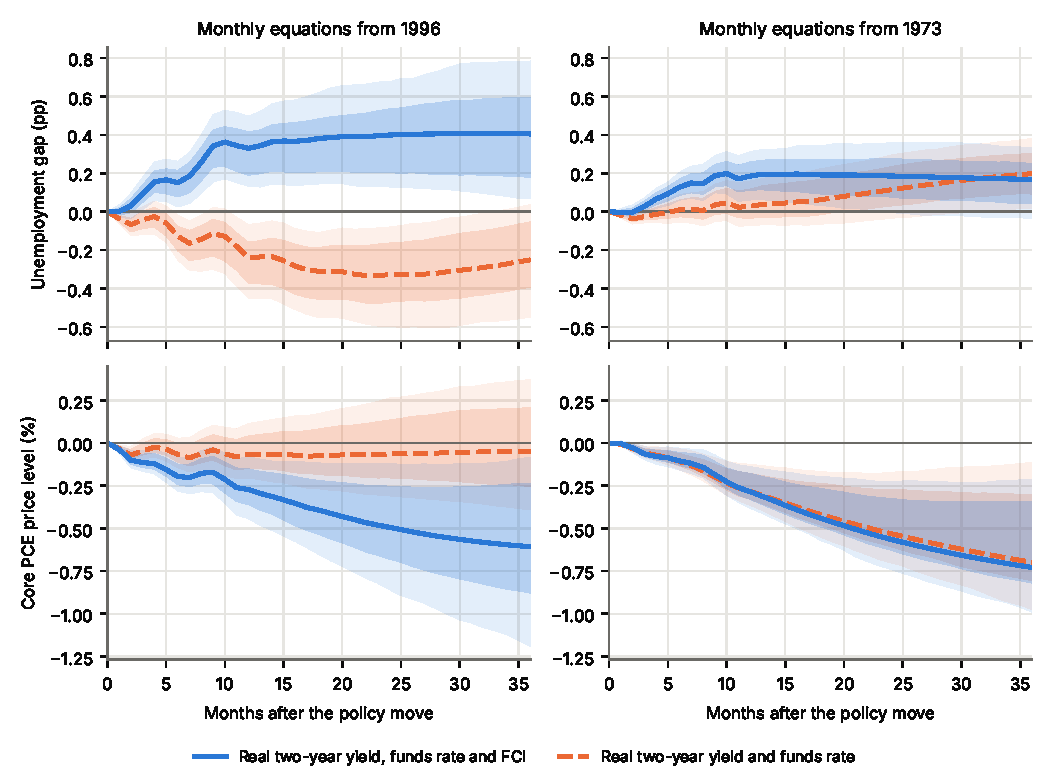
\includegraphics[width=\textwidth]{../baseline_real/report/fig_intro.pdf}
\caption{Responses to a Policy Move That Raises the Two-Year Yield 1 Percentage Point}
\label{fig:intro}
\begin{flushleft}\footnotesize\textit{Notes:} The move occurs in the window around the announcement. Blue: the surprise carried through the real two-year yield, the real federal funds rate and the real financial conditions index. Orange dashed: carried through the two real rates alone. Left: monthly equations estimated from 1996; right: from 1973. Same surprise (the 252 announcements of 1996--2026), normalization, 12 monthly lags and bootstrap draws within each sample; March--December 2020 dropped. Shaded bands: 68 and 90 percent intervals.\end{flushleft}
\end{figure}

Four main conclusions emerge.
\begin{enumerate}\setlength\itemsep{0pt}
\item \textbf{Adding financial conditions reverses the estimated unemployment response.} In the data since 1996, where the wrong-signed response appears, adding financial conditions raises the two-year unemployment response by \bl{dc:nom:AC:u:24} and \bl{dc:real:AC:u:24} percentage point in the nominal and real versions, holding the surprise, sample and lag length fixed. With real rates and the FCI in the model, a tightening raises unemployment and lowers prices after a year in every robustness test, from either starting date.
\item \textbf{Measuring rates in real terms matters for prices over the long sample.} Since 1996 the nominal and real versions give nearly the same responses. From 1973, when expected inflation moved far more, the real version gives a price fall about as large as since 1996, and the nominal version a much smaller one.
\item \textbf{Lowering inflation costs less unemployment than recent estimates imply.} The sacrifice ratio of about one percentage-point year per 1 percent of the price level is a small fraction of the value of about 7 implied by high-frequency estimates for 1990--2008 \citep{barnichon2021}, and close to estimates for the decades before 1990.
\item \textbf{Policy surprises are a modest source of fluctuations.} Announcement surprises explain almost none of the variation in unemployment and inflation. Surprises in the policy direction on every day explain about 5 percent of the variation in inflation, and they mark the Volcker tightening and the easing and tightening of the 2020s; the easing added about \bl{dc:hist:pi2122} percentage point to core inflation in 2021--22.
\end{enumerate}

The approach has three features. First, I measure the effect of each surprise in a short window around the announcement, when unemployment and inflation cannot move, and carry it forward in a daily and a monthly model estimated on ordinary data. As in \citet{jacobson2026}, the model takes into account when each announcement falls within its month. Second, financial conditions enter as a whole, as the transmission mechanism of standard models implies \citep{boivin2010}. The FCI combines the 10-year yield, equity valuation and the real dollar, weighted by their responses to policy news. The two-year yield and the federal funds rate enter beside it, so the model contains the policy rate and a market rate that stays informative when the policy rate is at its lower bound. Third, I measure rates and the index in real terms, removing expected inflation, which trended down from the 1980s to the 1990s while activity did not.

The results give the index of my companion paper \citep{fcinote} a use beyond describing conditions. Measured in units of a policy move, financial conditions are the variable that standard estimates of transmission leave out.

Section~\ref{sec:tests} tests the approach. With credit spreads added, in the monthly or the daily block, unemployment still rises and prices still fall. Estimating the financial dynamics on daily data, in the spirit of the correction of \citet{jacobson2026}, adds most to the response once financial conditions are measured; without them unemployment still falls. Section~\ref{sec:rob} varies the sample, the variables, the surprise and the lag length. Section~\ref{sec:shares} uses the estimates to ask how much surprises in the policy direction explain of the fluctuations in unemployment and inflation. Section~\ref{sec:slow} turns to slow-moving rates: measuring rates relative to estimates of the neutral rate gives responses at least as large, with the same effect of adding the FCI under three estimates, and a flexible time trend gives smaller ones since 1996, which marks the treatment of trends as a question for further work.

\subsection{Connection to the Literature}
\textbf{Surprises and their effects.} Interest-rate surprises around FOMC announcements were meant to settle the measurement problem. The decision precedes the announcement, so market moves in a narrow window around it cannot have caused it \citep{kuttner2001,gurkaynak2005}. Such surprises measure the effects of policy on asset prices well \citep{bernanke2005,hanson2015,nakamura2018,swanson2021}, but for unemployment and inflation the old puzzles often return. Four explanations have been offered, each with a fix. Announcements reveal the Fed's view of the economy, and separating that information gives larger price effects \citep{romer2000,nakamura2018,jarocinski2020,miranda2021}. Part of each surprise is predictable, and removing it sharpens the estimates \citep{bauer2023,bauer2023aer}. Markets react in minutes while unemployment and inflation are monthly averages, and measuring inflation daily removes most of the wrong sign \citep{jacobson2026}. And credit costs, stock prices and the dollar carry part of the effect \citep{gertler2015,caldara2019,kroencke2021,bauer2023jep,boehm2024,bauer2026,boehm2026}. The specifications that produce these puzzles carry the surprise forward through one or two interest rates.

\textbf{What is new.} Unlike \citet{gertler2015} and \citet{caldara2019}, who add a credit spread to a VAR in interest rates, I hold fixed the direction of policy news that the announcement window identifies and vary which financial prices carry it forward: rates alone, or rates and a broad index of long yields, equity valuations and the dollar. My paper is closest in spirit to \citet{jacobson2026}. Like them, I hold the surprise and the method fixed and change one measurement. They show that averaging daily data into months biases the estimated effects of policy, and they remove most of the price puzzle by measuring inflation with a daily price index. I change how the channel from policy to the economy is measured, and my main result is for activity. The two corrections are complementary. My model estimates the financial dynamics on daily data and tracks when in the month each announcement falls, as they recommend; the daily dynamics, not the calendar position, raise the unemployment response once financial conditions are in the model (Section~\ref{sec:timingtest}). Omitted financial channels and temporal aggregation are two sources of the puzzles, and correcting both gives the largest responses. \citet{bauer2023} and \citet{jarocinski2020} improve the surprise itself. In my design a surprise enters only through its immediate effect on rates and the FCI and through its timing, so their fixes and mine can be combined, and Section~\ref{sec:rob} does so.

\textbf{Financial channels and risk appetite.} \citet{gertler2015} show that policy surprises that move short rates modestly produce large movements in credit costs, through term premia and credit spreads. \citet{caldara2019} find that the response of activity to policy is weak and imprecise without a measure of credit spreads and conventional with it. \citet{bauer2026} find that monetary transmission appears to operate primarily through risk appetite and risk asset prices. These findings are consistent with mine. My index includes equity valuations, which move with risk appetite, but they also move with expected cash flows, so the model does not attribute the response to risk appetite in particular. The 10-year yield carries the term premium, and equity valuation carries the risk premium on the claims of firms that borrow. Credit spreads have no intraday series, so their response to policy news cannot be measured in the window, and a parsimonious index weighted by its response to policy keeps out movements unrelated to policy. Section~\ref{sec:credit} adds a daily credit spread, and a tightening still raises unemployment and lowers prices. Studies of the ``non-yield'' shock treat policy-driven moves in stock prices and the dollar as a second shock \citep{bauer2026,boehm2024}. \citet{boehm2026} select the combination of two yield-curve surprises and the non-yield shock that best accounts for macroeconomic fluctuations; they choose the direction of the shock for its macroeconomic content. I fix the conventional direction, news about the path of interest rates, and ask which financial variables are needed to trace it. My estimates are therefore conditional on that direction of news; they do not apportion business-cycle fluctuations among the shocks that announcements contain.

\FloatBarrier
% ============================================================
\section{Financial Conditions and the Empirical Approach}\label{sec:data}
This section explains why financial conditions should matter for the effects of policy, builds the index that measures them, sets out what announcement windows reveal and the identifying assumptions, and describes the model.

\subsection{Why Financial Conditions Matter for Monetary Policy}\label{sec:background}
The workhorse evidence on policy comes from VARs with a few macroeconomic variables and one interest rate \citep{bernanke1992,christiano1999}. Some studies add a credit spread \citep{gertler2015,caldara2019}, and factor models bring in many more series \citep{bernanke2005favar}. Long yields, equity valuations and the dollar are usually absent. A rise in the two-year yield on the day of an announcement comes with a large tightening of broader financial conditions, because a surprise about the path of policy moves long yields, stock prices and the dollar together. A model that observes only rates estimates how the economy responds to them from all the days and months in the sample. If unemployment responds to financial conditions and not directly to the policy rate, the rate stands in for financial conditions, and the error contains past financial shocks that a VAR with few lags cannot capture (Appendix~\ref{app:toy}; \citealp{fernandez2007}). Whether this matters in practice is an empirical question, which the matched comparison of Section~\ref{sec:baseline} answers. A simulation shows what to expect. When the model with financial conditions generates the data, the same model estimated without the FCI gives a median unemployment response of the wrong sign after 12 months (\bl{sim:main_nofci:u12:med} percentage point, against a true \bl{sim:main_fci:u12:truth}), and adding the FCI raises the 24-month response in nearly every simulated sample (Appendix~\ref{app:relation}). This differs from the omitted information about the economy that \citet{sims1992} proposed to explain the price puzzle; here the omitted variables are the channel itself.

Which financial prices move matters because they reach spending through different channels. Few households and businesses borrow at the policy rate. A household financing a home faces a mortgage rate tied to long yields; a firm valuing an investment faces a cost of capital set by long yields and equity prices; an exporter faces the dollar. Arbitrage links these rates to current and expected short rates. Higher rates raise the cost of capital and lower the value of existing capital \citep{jorgenson1963,hall1967,tobin1969}. Lower stock prices lower wealth and consumption \citep{ando1963,friedman1957}. A stronger dollar shifts spending toward imports \citep{fleming1962,mundell1963}. Modern models of the business cycle contain the same links \citep{christiano2005,smets2007,gali2005,kaplan2018,auclert2019}, and the effects come with a lag \citep{friedman1961}. The FOMC describes its policy in the same terms, as working through broad financial conditions.

Broad financial conditions indexes summarize this transmission \citep{hatzius2010,brave2011,ajello2023}, and credit spreads and asset prices help predict activity \citep{gilchrist2012,stock2003}. Such correlations need not be causal, because financial conditions also respond to the economy. The literature on high-frequency surprises has the opposite strength and weakness: it identifies policy shocks cleanly but carries them through few variables. I combine the two. The weights of my index come from how its components respond to policy news, and the surprise is carried forward through the estimated relationship between that index and the economy.

\textbf{Why real.} What matters in these models is the real rate, not the nominal rate: a given nominal yield is tighter when expected inflation is low. The distinction matters most for inflation over long samples. Nominal rates and inflation fell together from the early 1980s, so a model in nominal rates partly links low rates to low inflation through that common trend rather than through policy.

\subsection{The Financial Conditions Index}\label{sec:measure}
The FCI is the market index of my companion paper, \citet{fcinote}, which derives its weights and compares it with other indexes. I apply its method to the announcements of this paper. Indexes of this kind are weighted sums of financial variables, and they differ mainly in where the weights come from \citep{hatzius2010}. The best known in markets is the Goldman Sachs index \citep{dudley2000,hatzius2018}, whose published weights fall on the federal funds rate, the 10-year yield, a corporate spread, equity valuation and the dollar. FCI-G takes its weights from large macroeconomic models \citep{ajello2023}. Mine come from event-study regressions, long used to measure how asset prices respond to policy \citep{kuttner2001,bernanke2005,hanson2015,nakamura2018}.

\textbf{Why announcement windows.} The approach relies on one fact. In a narrow window around an FOMC announcement, the yield, stock prices and the dollar are all observed at high frequency, and policy news is the main systematic force moving them. The windows therefore reveal how the three respond to policy, and how large their joint movement is, without waiting for the economy to react. Unemployment and inflation cannot move in the window.

\textbf{Policy news.} Let $\Delta X_a$ be the $5\times 1$ vector of changes in the window around announcement $a$ in the surprise to the funds rate set at the meeting and at the next meeting, implied by federal funds futures scaled for the days left in the contract month (MP1 and MP2), and in the second to fourth quarterly eurodollar futures, replaced by the matching SOFR futures from January 2022 \citep{acosta2025}. Following \citet{nakamura2018}, let $p_a$ be the first principal component of these changes, signed so that it moves with the fourth eurodollar future. Policy news is $p_a$ rescaled so that one unit moves the two-year yield $y^{2}$ by 1 percentage point, in a regression with a constant:
\begin{equation}
s_a = \gamma\, p_a, \qquad \gamma = \frac{\sum_a (p_a-\bar p)(\Delta y^{2}_a-\overline{\Delta y^{2}})}{\sum_a (p_a-\bar p)^{2}}. \label{eq:ns}
\end{equation}

\textbf{Weights.} Let $\Delta A_a$ be the vector of changes in the 10-year yield, the S\&P 500 and the dollar index (DXY) in the window. Following the companion paper, I treat these changes as
\begin{equation}
\Delta A_a = \psi\, s_a + \eta_a, \label{eq:window}
\end{equation}
where $\psi$ holds the policy responses and $\eta_a$ is other news, with covariance matrix $\Sigma$. I estimate $\psi$ by regressing each element of $\Delta A_a$ on $s_a$ and a constant, and $\Sigma$ from the residuals, over the 252 announcements from January 1996 to July 2026 that I use throughout.\footnote{The companion paper also uses the announcement of September 2026 and scales $s_a$ without a constant. Its weights differ from mine by about 1 percent.} The weights are those that recover the policy component most precisely (one-factor generalized least squares):
\begin{equation}
w = \frac{\Sigma^{-1}\psi}{\psi'\Sigma^{-1}\psi}. \label{eq:weights}
\end{equation}
An asset gets more weight when it responds strongly to policy news and moves little for other reasons in the window, so the index is the combination of the three that tracks policy news most closely. Because $w'\psi=1$ and $s_a$ is scaled to the two-year yield, a policy move that raises the two-year yield 1 percentage point raises the index by 1 unit. The weights are 0.62 on the 10-year yield, $-0.052$ per percent on stock valuations and 0.066 per percent on the dollar, and each of the three accounts for about a third of the index's response to policy (Table~\ref{tab:weights}). Consider a hawkish surprise that raises the two-year yield 1 percentage point. On average it raises the 10-year yield about \bl{rv:psi:y10} percentage point, lowers stock valuations about \bl{rv:psi:equities} percent and raises the dollar about \bl{rv:psi:dollar} percent. Higher long rates raise the cost of borrowing for homes and investment, lower stock prices cut household wealth and raise the cost of equity, and a stronger dollar makes exports less competitive. The index adds these three tightenings into one number in units of the two-year yield. These shares describe how the three asset prices move on announcement days; the monthly equations assume that the three affect the economy in the same proportions.

\begin{table}[tp]\centering\small
\caption{Market-Index Weights from Policy News}\label{tab:weights}
\resizebox{\ifdim\width>\textwidth\textwidth\else\width\fi}{!}{%
\begin{tabular}{lrrr}\toprule Component & Response to policy news & Weight & Share of a policy move\\ \midrule
10-year Treasury yield (pp) & $+$0.53 (0.06) & $+$0.616 & 0.33\\
Equity valuation, 100 ln CAPE (\%) & $-$7.71 (0.95) & $-$0.052 & 0.40\\
Real broad dollar, 100 ln (\%) & $+$4.18 (0.54) & $+$0.066 & 0.27\\
\bottomrule\end{tabular}}
\begin{flushleft}\footnotesize\textit{Notes:} Response of each announcement-window change (USMPD monetary-event window: from 10 minutes before the statement to 20 minutes after it, or to 60 minutes after the start of the press conference) to the policy-news factor (scaled so the 2-year yield moves 1 pp), with robust standard errors; weights from the one-factor GLS of Kiley (2026); share = weight $\times$ response (the three shares sum to 1).\end{flushleft}
\end{table}


In month $t$, the index in version $v$ is
\begin{equation}
F_t^{v} = w_B\, B_t^{v} + w_Q\, Q_t + w_D\, D_t, \label{eq:fci}
\end{equation}
measured as a deviation from its sample mean. Here $B_t$ is the 10-year yield, $Q_t=100\ln\text{CAPE}_t$ is the log of the cyclically adjusted price-earnings ratio and $D_t$ is 100 times the log of the real broad dollar. The index comes in two versions, which differ in how the yield is measured.

\textbf{The nominal version.} The nominal version uses the nominal 10-year yield, $B_t=y^{10}_t$. It is the natural point of comparison with indexes built from nominal variables, and it has one problem: a trend. Nominal yields carry the inflation of the period. The 10-year yield was very high in the early 1980s, when expected inflation was high, and fell for decades after. Stock valuations moved the other way: CAPE was low in the early 1980s and rose over the following decades. With a positive weight on the yield and a negative weight on valuation, both movements read as a steady loosening of conditions, and a linear trend alone explains \bl{tr:n:r2} percent of the variance of the nominal version since 1973.

\textbf{The real version.} The real version subtracts 10-year expected inflation $\pi^{10}_t$ from the yield, $B_t=y^{10}_t-\pi^{10}_t$, and leaves stock valuation as it is, because CAPE is already a real measure. It removes the inflation in the yield, and with it part of the drift: a linear trend explains \bl{tr:r:r2} percent of its variance. The rest of the drift comes from real rates and valuations, which trended with the neutral rate; Section~\ref{sec:slow} returns to it.

\textbf{The two-year yield and the funds rate.} The two-year yield and the federal funds rate are adjusted in the same two versions. With $y^{2}_t$ the nominal two-year yield, $i_t$ the effective funds rate and $\pi^{2}_t$ two-year expected inflation \citep[from the Cleveland Fed;][]{haubrich2012},
\begin{equation}
R_t^{\text{nominal}} = y^{2}_t, \quad R_t^{\text{real}} = y^{2}_t - \pi^{2}_t, \qquad I_t^{\text{nominal}} = i_t, \quad I_t^{\text{real}} = i_t - \pi^{2}_t. \label{eq:twoyear}
\end{equation}
The funds rate is deflated with the same two-year expectation. From 1982 the expectations are the Cleveland Fed's. Before 1982 I use the Livingston Survey, which asks economists for their expected CPI inflation over the next 12 months; that one-year expectation stands in for all three horizons. For the two-year yield and the funds rate this is a short-horizon measure for a short-horizon rate. For the 10-year yield it lets long-run expectations in the 1970s move one for one with short-run ones, which affects the real FCI before 1982 but not the real two-year yield. Expected inflation is monthly and moves slowly; the daily series add its interpolated monthly values to daily market prices, so day-to-day moves come from markets.\footnote{Appendix~\ref{app:details} describes the splice of the Livingston and Cleveland series and the construction of the daily series.}

\textbf{Two rates.} The model contains both the two-year yield and the funds rate. The funds rate is the instrument of policy. The two-year yield summarizes the expected path of the funds rate over the next two years, and it remains informative when the funds rate cannot move. The funds rate was at its effective lower bound in 2008--2015 and 2020--2021 (a monthly average below 0.25 percent in \bl{zlb:n} months, \bl{zlb:share96} percent of the months since 1996 and \bl{zlb:share74} percent of those since 1974). In those years policy worked through expectations of the future path of rates, and \citet{swanson2014} find that the one- and two-year yields stayed surprisingly responsive to news in 2008--2010 and became more constrained only from late 2011. I therefore measure the surprise and its effects per percentage point on the two-year yield, and include the funds rate so that the model can separate the rate the FOMC sets from the expected path. The lower bound matters more in the sample since 1996, where its months are a larger share.

Figure~\ref{fig:fcis} plots the versions of the index. The versions do not differ at high frequencies; the correlation of 12-month changes is \bl{fci:c12:nr} between the nominal and real versions. The differences are slow. The real version is below the nominal one by about 2 units around 1980, when expected inflation was highest, and the two are close after 1990.

\textbf{Comparison with the Goldman Sachs index.} A widely followed index offers a check on whether the approach captures what market participants mean by financial conditions. The companion paper rebuilds the Goldman Sachs index from public data with its published weights and shows that the rebuild mimics the published series closely \citep{fcinote}. The two indexes agree on changes: the correlation of 12-month changes is \bl{gs:n:l:chg} for the nominal versions and \bl{gs:r:l:chg} for the real versions from 1974. In levels the nominal versions agree since 1996 (\bl{gs:n:p:lev}) but less in 1974--95 (\bl{gs:n:e:lev}), when the two weight the inflation trend differently; the real versions agree closely throughout (\bl{gs:r:l:lev}). The close agreement in levels partly reflects shared inputs and a shared trend, so it shows that the measures agree, not that either is the right one for transmission. The agreement in changes, from weights derived in very different ways, is the more informative fact (Appendix Figure~\ref{fig:gs}).

\begin{figure}[tp]
\centering
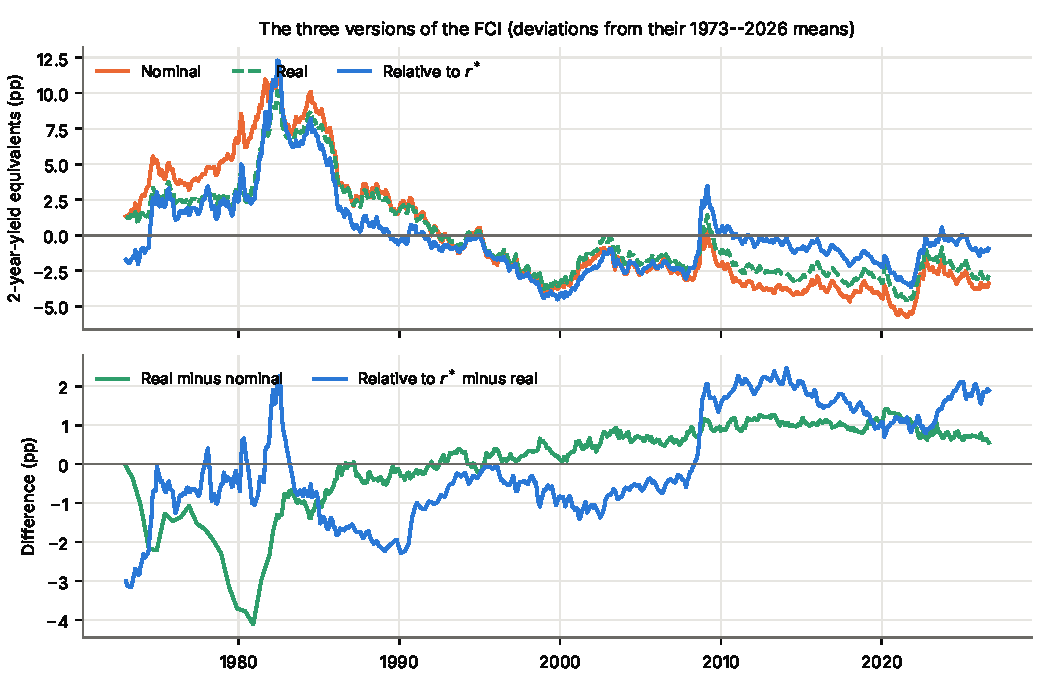
\includegraphics[width=0.9\textwidth]{../baseline_real/report/fig_fcis.pdf}
\caption{Versions of the FCI}
\label{fig:fcis}
\begin{flushleft}\footnotesize\textit{Notes:} Monthly, in two-year-yield equivalents (a policy move that raises the two-year yield 1 percentage point raises each by one unit in the window). Each series is shown as a deviation from its mean over January 1973 to September 2026. The version relative to $\rs$ is the one of Section~\ref{sec:slow}. Lower panel: real minus nominal, and relative to $\rs$ minus real.\end{flushleft}
\end{figure}

\subsection{What the Windows Show and the Identifying Assumptions}\label{sec:timing}
The shock is the Nakamura--Steinsson policy-news surprise, $s_a$ in equation~\eqref{eq:ns}, from the San Francisco Fed's U.S.\ Monetary Policy Event-Study Database \citep{acosta2025}. I use the 252 FOMC announcements from January 1996 to July 2026 with all the window measures available (Appendix~\ref{app:details}). The window runs from 10 minutes before the statement to 60 minutes after the press conference starts, or 30 minutes around the statement when there is no press conference. Identification comes from timing, at three frequencies, summarized in Table~\ref{tab:timing}.

\begin{table}[tp]\centering\small
\caption{Timing Assumptions}\label{tab:timing}
\begin{tabular}{p{0.12\textwidth}p{0.29\textwidth}p{0.38\textwidth}p{0.09\textwidth}}\toprule
Frequency & What can move & Assumption & Equation \\\midrule
Window (minutes) & Two-year yield, FCI and funds rate, by the amounts measured in the window & News about the path of interest rates is the main systematic force in the window, and the only one correlated with the surprise. Unemployment and inflation do not move. & \eqref{eq:impact} \\[3pt]
Daily & Two-year yield, FCI and funds rate, each day after the announcement & They depend on their own recent history and on the unemployment and inflation of this month and last month. & \eqref{eq:daily} \\[3pt]
Monthly & Unemployment and inflation, from the month after the announcement & Within a month, unemployment and inflation are set first. They respond to financial variables only with a lag of at least one month. & \eqref{eq:monthly} \\\bottomrule
\end{tabular}
\end{table}

\textbf{The window.} The window move in the FCI is computed with the weights in equation~\eqref{eq:weights}:
\begin{equation}
\Delta F_a = w_B\, \Delta y^{10}_a + w_Q\, \Delta \text{SP}_a + w_D\, \Delta \text{DXY}_a. \label{eq:winfci}
\end{equation}
These are the measures available within the day, and the ones used to estimate the weights. Percent changes in the S\&P 500 equal percent changes in CAPE within a window, because earnings are fixed. I express all effects per percentage point on the two-year yield in the window. The effect on each variable is the ratio of two regression slopes on the surprise, an instrumental-variables estimate with $s_a$ as the instrument:
\begin{equation}
b = \begin{pmatrix} 1 \\ b_F \\ b_I \end{pmatrix}, \qquad b_F = \frac{\sum_a (\Delta F_a - \overline{\Delta F})\,(s_a-\bar s)}{\sum_a (\Delta y^{2}_a - \overline{\Delta y^{2}})\,(s_a-\bar s)} = 1, \qquad b_I = \frac{\sum_a (\Delta f^{1}_a - \overline{\Delta f^{1}})\,(s_a-\bar s)}{\sum_a (\Delta y^{2}_a - \overline{\Delta y^{2}})\,(s_a-\bar s)} = \bl{ff:b}. \label{eq:impact}
\end{equation}
The FCI's ratio is one because the scaling in equation~\eqref{eq:ns}, the weights and this ratio use the same announcements and regressions with a constant. The funds rate's ratio is an estimate: $\Delta f^{1}_a$ is MP1, the surprise to the funds rate set at the meeting, implied by the current-month federal funds future scaled for the days left in the month, so a surprise that raises the two-year yield 1 percentage point raises the expected funds rate \bl{ff:b} percentage point. The funds rate itself confirms the size: per percentage point on the two-year yield in the window, the effective funds rate rises \bl{ff:dff1} percentage point from the day before the announcement to the day after and \bl{ff:dff22} by a month later. At the lower bound the futures barely move, and so the funds rate does not either. Expected inflation moves slowly, so I take the window move to be the same in both versions: the real impacts assume that expected inflation does not move within the window.

\textbf{How much the surprise explains.} The interest-rate surprise explains \bl{r2:y2} percent of the window variation in the two-year yield and \bl{r2:fci} percent of the variation in the FCI, but only \bl{r2:y10} percent for the 10-year yield, \bl{r2:sp} percent for the S\&P 500 and \bl{r2:usd} percent for the dollar. Announcements move stock prices and the dollar by more than interest-rate surprises explain \citep{boehm2024,bauer2026}. The unexplained part is either news unrelated to policy, in which case my estimates capture the effects of policy, or policy news that does not move interest rates, in which case they capture one dimension of policy news and the effects of all of it could be larger. Both readings agree on the channel: policy news reaches the economy through broad financial conditions.

\textbf{The day.} On the announcement day, the two-year yield, the FCI and the funds rate shift by the vector $b$. I use the window move and not the change over the whole day, because the full-day change contains other news. On later days the three series move as equation~\eqref{eq:daily} implies. They affect each other only through the daily lags, so no ordering among them is needed within the day.

\textbf{The month.} Within each month, unemployment and inflation are set first, and markets then respond to them. In the month of the announcement, unemployment and inflation therefore have not moved. They respond from the next month on, through the monthly average of the daily financial series. That average depends on when in the month the announcement falls, since an announcement late in a month affects few days of that month's average. This is how the model takes the timing of announcements into account, as \citet{jacobson2026} recommend. The ordering is the familiar recursive one, in which slow-moving macroeconomic variables come before financial variables \citep{bernanke1992,christiano1999}. The daily equations include the current month's unemployment and inflation, even though those figures are published later. I treat the monthly values as a summary of conditions that markets observe as the month unfolds.

\textbf{The main assumption.} The design thus has three steps: identify policy news in the window, measure its immediate financial effect $b$, and propagate that effect through daily and monthly equations estimated on ordinary days and months. Only the first two steps use the announcements. The third carries the main assumption: once the shock is identified, the economy responds to a change in the financial variables in the same way whatever caused it. A shock identified by a Cholesky ordering or an external instrument is carried through the same estimated dynamics as every other shock, and I do the same. Suppose stock prices fall 5 percent in an announcement window because the surprise raises the rate at which future earnings are discounted. On another day they fall 5 percent because earnings forecasts are cut. The first fall raises the cost of capital and lowers wealth with no news about demand. The second may also signal weaker demand, which would lower activity whatever the policy rate does. The model carries both through one equation. If the discount-rate fall is more or less contractionary than the average fall, the estimated propagation is wrong for the policy surprise. Section~\ref{sec:resolve} checks the financial part of this assumption: measured from the close before each announcement, the yield and the FCI move in the following weeks as the model predicts. This problem differs from central-bank information, which concerns what $s_a$ reveals in the first step. \citet{bauer2023aer} show that what looks like an information effect largely reflects the Fed and markets responding to the same economic news, so that the surprises can be treated as policy news once that response is accounted for. I therefore use the surprises as they are. Section~\ref{sec:surprise} confirms that the results hold with their cleaned surprise, and Appendix~\ref{app:further} with the sign restriction of \citet{jarocinski2020}.

Two further assumptions are specific to this paper. First, the surprise reaches unemployment and prices only through the two rates and the FCI, and has no direct effect on them in the window. Other channels, such as credit spreads and expectations, are left out; Section~\ref{sec:credit} adds them. So are moves in stock prices and the dollar that are unrelated to $s_a$. The non-yield shock of \citet{boehm2024} is uncorrelated with policy-news surprises, so such moves do not bias $b_F$. Second, the monthly equations see the FCI as a single index: the 10-year yield, equity valuation and the dollar affect unemployment and prices in proportion to their weights. The companion paper examines how the weights and the choice of assets change the index \citep{fcinote}.

\subsection{A Mixed-Frequency VAR}\label{sec:midas}
Financial markets process policy news in minutes, while unemployment and prices take months to respond. The model therefore runs on two clocks. A daily block tracks the immediate repricing of the two-year yield, the FCI and the funds rate and how long that repricing lasts. A monthly block measures how the accumulation of these daily conditions shifts unemployment and inflation, which in turn feed back into the markets of the following month. The announcement enters on the day it occurs, so the model knows whether a surprise came early in a month, when it moves most of that month's financial conditions, or late, when it moves few of them.

\textbf{Structure.} Let $x_\tau=(R_\tau,F_\tau,I_\tau)'$ hold the two-year yield, the FCI and the funds rate on day $\tau$, in the same version. Let $m_t=(U_t,\pi_t)'$ hold the two monthly variables. The unemployment gap $U_t$ is the unemployment rate minus the CBO estimate of its natural rate. The CBO estimate does not respond to the surprise, so the response of the gap equals that of the unemployment rate. Inflation is $\pi_t=1200\,\Delta\ln P_t$, where $P_t$ is the price index for personal consumption expenditures excluding food and energy (core PCE).

The daily block is a VAR that uses averages of the past day, week, month and quarter as regressors \citep{corsi2009}:
\begin{equation}
x_\tau = \alpha + \sum_{k\in\{1,5,22,66\}} \Phi_k\, \bar x_{\tau-1}^{(k)} + \Gamma_0\, m_{t(\tau)} + \Gamma_1\, m_{t(\tau)-1} + \xi_\tau, \label{eq:daily}
\end{equation}
where $\bar x_{\tau-1}^{(k)}$ is the average of $x$ over the $k$ days through $\tau-1$, and $t(\tau)$ is the month of day $\tau$. Averages over about a day, a week, a month and a quarter capture persistence with few coefficients, which matters because how long the financial movement lasts determines how much of it reaches the monthly averages. When the FCI is left out, $x_\tau$ holds the two rates alone. The equation for the funds rate is linear, so the model does not impose the lower bound; during the lower-bound years the funds rate barely moved, and its daily equation learns that from the data.

The monthly block is
\begin{equation}
m_t = c + \sum_{l=1}^{L} A_l\, m_{t-l} + \sum_{l=1}^{L} G_l\, \bar x_{t-l} + \zeta_t, \qquad \bar x_{t}=\frac{1}{n_t}\sum_{\tau\in t} x_\tau, \label{eq:monthly}
\end{equation}
with $n_t$ the number of weekdays in month $t$. The model is a mixed-frequency VAR \citep{ghysels2016}. The equation contains no current-month term in $\bar x_t$, which is the timing assumption of Table~\ref{tab:timing}. The monthly equations contain a constant and no time trend; Section~\ref{sec:slow} adds one.

\textbf{How the responses are computed.} The response to a policy surprise is traced day by day. On the announcement day the two rates and the FCI jump by the window impact $b$ and the macro variables are at their no-surprise values. Each later day, the daily equation gives the three financial series from their own recent averages and from the macro variables of the month. At the end of each month the monthly average of the daily financial series enters the monthly equations, which give the next month's unemployment and inflation. Those feed back into the daily equations of the following month. The response is the difference from a path with no surprise. Because the model is linear, the response to a surprise of any size is a multiple of the response to a unit surprise. I average the responses over the positions of the announcements within their months, as in the data, because an announcement early in a month moves that month's average more than a late one. The response of the price level after $h$ months is $\sum_{j=0}^{h}\tilde\pi_j/12$.

\textbf{Relation to a monthly VAR.} If every announcement fell on the first day of its month and the daily block were replaced by a monthly equation, the model would be a standard monthly VAR with a recursive ordering. The daily block adds the position of each announcement in its month and the fast dynamics of the financial variables, which it estimates on many more observations. A proxy VAR instead estimates the effect of the surprise on every variable from monthly residuals. Two facts favor starting the system from the window. The surprise is a weak instrument for monthly residuals, so a proxy VAR has wide sets, and a direct projection of the outcomes on the surprise is imprecise and changes sign with its controls. Measuring the impact in the window, where the surprise explains most of the movement, and estimating the propagation on ordinary data uses the information each source has. Section~\ref{sec:monthlyvar} estimates both monthly benchmarks, and Appendix~\ref{app:relation} gives the algebra.

\textbf{Why the window, and not monthly innovations.} A monthly VAR recovers a policy shock from the month's innovations, and that requires the shock to be a combination of those innovations (invertibility). Starting the model from the window does not: the shock is observed directly, and the model only has to propagate it. In these data the month's VAR innovations explain \bl{dc:diag:real:yes:1996:r2} percent of the variance of the month's summed surprises, and the shock recovered from them has a correlation of \bl{dc:diag:real:yes:1996:corr} with the surprise. The same happens in samples simulated from the model, where the policy shock is the window surprise by construction (median $R^2$ of \bl{dc:sim:r2_z_u:med} percent): a surprise concentrated on one day is weakly recovered from the innovations of its month.\footnote{Appendix~\ref{app:relation} reports this diagnostic for each version and both samples, with six months of later innovations added and with the simulation.}

\textbf{Estimation and inference.} I estimate each block by ordinary least squares. The daily block uses the weekdays from January 1996, the month of the first announcement with all window measures, to September 2026. The monthly equations have two samples, which give the two baselines: from January 1996 (\bl{nobs} months) and from January 1973 (\bl{b73:nobs} months). In the longer sample the months before 1990 use monthly series in place of the daily block (Appendix~\ref{app:details}); the daily block, the announcements and the window impacts are those of 1996--2026 in both. The lagged daily averages and the monthly lags may use earlier observations. Both blocks leave out March to December 2020, which is the same as a dummy for each of those months: the pandemic moved unemployment by more in those months than in any other episode, for reasons unrelated to financial conditions. The 2020 values still enter as lags, and Section~\ref{sec:rob} keeps them in. The baseline has $L=12$ monthly lags, fixed in advance; Section~\ref{sec:surprise} and Appendix~\ref{app:lags} report 6.

Intervals come from a block bootstrap with 500 draws \citep{kunsch1989,jentsch2019}. Each draw resamples the calendar months from 1996 in blocks of 12 and uses together the monthly residuals, the daily observations and the announcements of the months drawn. That keeps the dependence among them. In the sample from 1973 the residuals of the months before 1996 are drawn in blocks of 12 of their own. The monthly equations and the daily block are re-estimated on each draw. The intervals are bias-corrected percentile intervals \citep{efron1987}: in this model, as in other small-sample VARs \citep{kilian1998}, the draws are on average smaller than the estimates, and the correction centres the intervals on the estimates. The intervals hold the FCI weights at their estimates; re-estimating the weights in each draw leaves the responses after two years significant.\footnote{Appendix~\ref{app:boot} describes the bootstrap, compares the bias-corrected intervals with plain percentile intervals and with a simpler bootstrap, and reports the responses with the weights re-estimated.} A response is significant at the 5 or 10 percent level when its 95 or 90 percent interval excludes zero. I report 90 percent intervals, as recent studies in this area do \citep{bauer2023,caldara2019,miranda2021,ramey2016}, and 68 percent intervals, which \citet{jarocinski2020} report alongside them.

\textbf{Data.} All inputs are public series (Appendix~\ref{app:data}). Daily market data are the 2-year and 10-year Treasury yields, the effective federal funds rate, the S\&P 500 and the broad dollar index. Monthly data are the unemployment rate, the CBO estimate of its natural rate, core PCE inflation and expected inflation from the Cleveland Fed. Policy news comes from the San Francisco Fed's event-study database. For the sample from 1973, the months before 1990 use monthly series in place of the daily block. All monthly financial variables are monthly averages of the daily series, in the model and in every benchmark.

\FloatBarrier
% ============================================================
\section{Results}\label{sec:results}
% Numbers in this section are macros from baseline_real/report/numbers.tex; the qualitative claims are asserted in baseline_real/claims_real.py.
Three results follow. Standard methods, applied to my data since 1996, give a tightening the wrong effect on unemployment. Adding the FCI reverses it, by about the same amount with nominal or real rates, and over the longer sample from 1973 it adds to responses that already have conventional signs, for unemployment mostly in the first year. The responses with the FCI imply a moderate cost of lowering inflation.

\subsection{Standard Methods after the Early 1980s}\label{sec:standard}
Standard identification schemes have not delivered conventional effects of monetary policy in samples that start after the early 1980s. \citet{ramey2016} estimates the specification of \citet{christiano1999} on 1983--2007 and finds that ``the results change dramatically and imply that increases in the federal funds rate lower the unemployment rate''; other schemes she examines give contractionary shocks that look expansionary, as \citet{barakchian2013} found for 1988--2007, or a pronounced price puzzle. The literature reads this either as a change in the economy, with policy responding more systematically and expectations better anchored \citep{boivin2006,boivin2010,primiceri2005}, or as a failure of identification once policy became forward-looking \citep{barakchian2013}. One finding points to measurement. \citet{caldara2019} find, for 1994--2007 with a proxy SVAR that uses high-frequency surprises, that the response of industrial production is weak and uncertain without a credit spread (about $-0.2$ percent, with a credible set that includes positive values) and about $-0.75$ percent when a credit spread is added.

I start from two standard methods, estimated on my own data so that they compare directly with the model below. Both use the monthly unemployment gap, core PCE inflation and the monthly average of the two-year Treasury yield, the one policy rate of these specifications, with 12 lags, no trend and March to December 2020 left out, on the two samples of the model, from 1996 and from 1973. The first is the recursive (Cholesky) VAR of \citet{christiano1999}, with the policy rate ordered last; its responses are to a 1 percentage point rise in the monthly yield. The second is a proxy VAR \citep{stock2018,mertens2013,gertler2015} that uses the Nakamura--Steinsson surprise, summed over the announcements of the month, as an instrument for the policy rate; its responses are to a surprise that raises the yield 1 percentage point in the announcement window, the unit of the model.\footnote{A window move of 1 percentage point raises the month's average yield by about \bl{mo:win} in the model, because the announcement falls on average in the middle of the month. The first-stage $F$ statistic of the proxy VAR is \bl{st:prox:F} from 1996 and \bl{st:prox73:F} from 1973, so I report exact Anderson--Rubin sets, which stay valid when the instrument is weak \citep{montiel2021,lunsford2015,lewis2026,bauer2026}.} Figure~\ref{fig:standard} shows the responses since 1996, and Table~\ref{tab:standard} reports both samples.

\begin{figure}[tp]
\centering
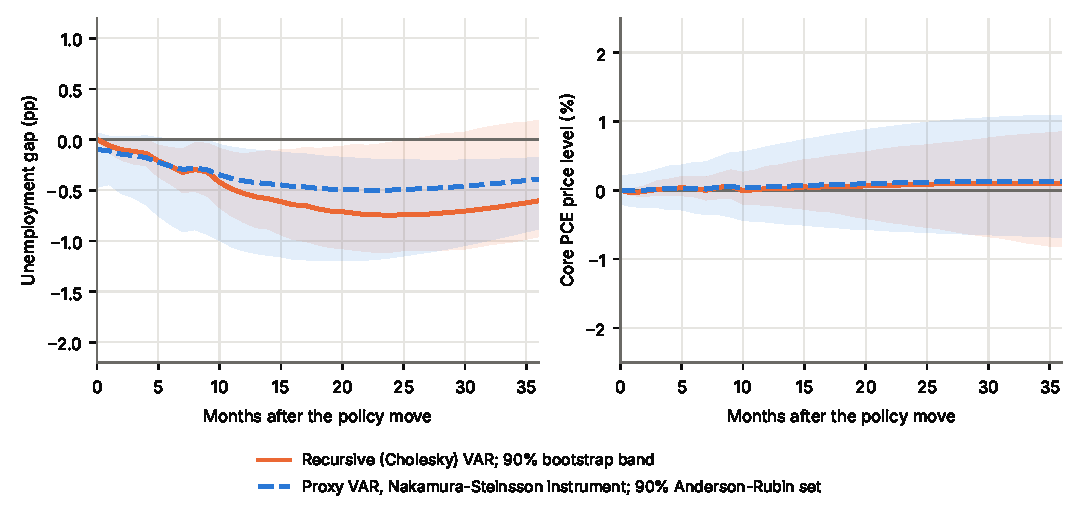
\includegraphics[width=\textwidth]{../baseline_real/report/fig_standard.pdf}
\caption{Standard Methods: Responses to a 1 Percentage Point Rise in the Two-Year Yield, 1996--2026}
\label{fig:standard}
\begin{flushleft}\footnotesize\textit{Notes:} Recursive (Cholesky) VAR and proxy VAR with the Nakamura--Steinsson instrument, in the monthly unemployment gap, core PCE inflation and the monthly average of the two-year yield; 12 lags; March--December 2020 dropped. Bands: 90 percent (bootstrap for the Cholesky VAR, Anderson--Rubin sets for the proxy VAR, truncated at $\pm4$).\end{flushleft}
\end{figure}

\begin{table}[tp]\centering\small
\caption{Standard Methods: Responses to a 1 Percentage Point Rise in the Two-Year Yield}\label{tab:standard}
\resizebox{\ifdim\width>\textwidth\textwidth\else\width\fi}{!}{%
\begin{tabular}{llcc}\toprule Method & Response & 1996--2026 & 1973--2026\\ \midrule
Recursive (Cholesky) VAR & Unemployment gap, 12 m & $-$0.53$^{*}$ & 0.12\\
 & & {\scriptsize [$-$0.87, $-$0.21]} & {\scriptsize [$-$0.06, 0.35]}\\
 & Unemployment gap, 24 m & $-$0.75$^{*}$ & 0.17\\
 & & {\scriptsize [$-$1.59, $-$0.40]} & {\scriptsize [$-$0.04, 0.41]}\\
 & Price level, 24 m & 0.08 & $-$0.08\\
 & & {\scriptsize [$-$0.50, 0.67]} & {\scriptsize [$-$0.50, 0.29]}\\
 & Price level, 36 m & 0.10 & $-$0.16\\
 & & {\scriptsize [$-$0.63, 1.00]} & {\scriptsize [$-$0.72, 0.47]}\\
\addlinespace
Proxy VAR & Unemployment gap, 12 m & $-$0.41$^{*}$ & $-$0.30\\
 & & {\scriptsize [$-$1.10, $-$0.09]} & {\scriptsize [$-$2.01, 0.13]}\\
 & Unemployment gap, 24 m & $-$0.50$^{*}$ & $-$0.19\\
 & & {\scriptsize [$-$1.17, $-$0.20]} & {\scriptsize [$-$1.48, 0.14]}\\
 & Price level, 24 m & 0.11 & 0.14\\
 & & {\scriptsize [$-$0.61, 0.97]} & {\scriptsize [$-$1.41, 2.32]}\\
 & Price level, 36 m & 0.13 & 0.21\\
 & & {\scriptsize [$-$0.68, 1.09]} & {\scriptsize [$-$1.81, 3.17]}\\
\bottomrule\end{tabular}}
\begin{flushleft}\footnotesize\textit{Notes:} Monthly VARs in the unemployment gap, core PCE inflation and the monthly average of the nominal two-year yield; 12 lags, constant, no trend, March--December 2020 dropped. Cholesky: the yield ordered last, per +1 pp innovation in the yield. Proxy VAR: Nakamura--Steinsson policy news summed within the month as instrument (first-stage $F$ = 5.6 from 1996, 3.8 from 1973), per +1 pp on the yield in the announcement window. Brackets: 90\% intervals (block bootstrap for the Cholesky VARs; exact Anderson--Rubin sets for the proxy VAR). $^{*}$ = excludes zero.\end{flushleft}
\end{table}


Since 1996 both reproduce the puzzle. Unemployment falls after a tightening, by \blabs{st:c2y96:u:12} percentage point after 12 months in the Cholesky VAR and \blabs{st:prox:u:12} in the proxy VAR, and it is still lower after 24 months. The price level does not respond. Starting in 1984 gives a smaller fall in unemployment, a funds-rate version on 1984--2007 gives the same sign, and adding commodity prices, the standard remedy for the price puzzle \citep{sims1992,ramey2016}, leaves the response negative (Appendix Tables~\ref{tab:standardall} and~\ref{tab:standardcom}). From 1973 the picture is different: the Cholesky VAR gives unemployment slightly higher and prices slightly lower after a tightening (\bl{st:c2y73:u:12} percentage point and \bl{st:c2y73:P:24} percent), and the proxy VAR, with an instrument that explains little of the monthly residuals over the long sample, is uninformative. The wrong signs are a feature of the sample since 1996 when the surprises are carried through interest rates alone.

\subsection{The FCI Model: Baseline Results}\label{sec:baseline}
Traced through the FCI, a tightening raises unemployment and lowers prices, with rates measured in nominal or in real terms. Table~\ref{tab:matched} gives the matched comparison for both samples: for each version, the responses after 24 months with the two rates alone and with the rates and the FCI, on common bootstrap draws within each sample.

\begin{table}[tp]\centering\footnotesize\setlength{\tabcolsep}{3pt}
\caption{Responses without and with the FCI after Two Years}\label{tab:matched}
\resizebox{\ifdim\width>\textwidth\textwidth\else\width\fi}{!}{%
\begin{tabular}{lcccc}\toprule
 & \multicolumn{2}{c}{Monthly equations from 1996} & \multicolumn{2}{c}{Monthly equations from 1973}\\ \cmidrule(lr){2-3}\cmidrule(lr){4-5}
Yield measure & Yield alone & Yield and FCI & Yield alone & Yield and FCI\\ \midrule
\multicolumn{5}{l}{\textit{A. Unemployment gap (percentage points)}}\\
Nominal & $-$0.35$^{**}$ & 0.40$^{**}$ & 0.13 & 0.12\\
 & {\scriptsize [$-$0.66, $-$0.06]} & {\scriptsize [0.09, 0.65]} & {\scriptsize [$-$0.05, 0.32]} & {\scriptsize [$-$0.07, 0.27]}\\
\textbf{Real} & \textbf{$-$0.33$^{**}$} & \textbf{0.40$^{**}$} & \textbf{0.11} & \textbf{0.19}\\
 & {\scriptsize [$-$0.60, $-$0.08]} & {\scriptsize [0.13, 0.68]} & {\scriptsize [$-$0.03, 0.29]} & {\scriptsize [0.00, 0.36]}\\
\addlinespace
\multicolumn{5}{l}{\textit{B. Core PCE price level (percent)}}\\
Nominal & $-$0.05 & $-$0.49$^{*}$ & $-$0.11 & $-$0.22\\
 & {\scriptsize [$-$0.36, 0.40]} & {\scriptsize [$-$0.80, $-$0.03]} & {\scriptsize [$-$0.32, 0.24]} & {\scriptsize [$-$0.40, 0.06]}\\
\textbf{Real} & \textbf{$-$0.06} & \textbf{$-$0.49$^{**}$} & \textbf{$-$0.53$^{**}$} & \textbf{$-$0.56$^{**}$}\\
 & {\scriptsize [$-$0.31, 0.26]} & {\scriptsize [$-$0.86, $-$0.12]} & {\scriptsize [$-$0.70, $-$0.17]} & {\scriptsize [$-$0.74, $-$0.23]}\\
\bottomrule\end{tabular}}
\begin{flushleft}\footnotesize\textit{Notes:} Responses 24 months after a policy move that raises the two-year yield 1 pp in the announcement window; 12 lags; March--December 2020 dropped; the shocks are the 252 announcements of 1996--2026 in both samples. Brackets: 90\% intervals; $^{**}$, $^{*}$: 5 and 10 percent levels. Paired differences (from 1996) are in Appendix Table~\ref{tab:matcheddiff}; 12 and 36 months and other lag lengths in Appendix Tables~\ref{tab:mainB} and~\ref{tab:lags}.\end{flushleft}
\end{table}


Start with the sample since 1996. With the rates alone the model gives what the standard methods give: unemployment falls, by \blabs{nom:no:u:24} percentage point after two years with nominal rates and \blabs{real:no:u:24} with real rates, and the price level does not respond. Adding the FCI moves both responses by nearly the same amount in both versions. It raises the unemployment response after 24 months by \bl{dc:nom:AC:u:24} and \bl{dc:real:AC:u:24} percentage point in the nominal and real versions, and it lowers the price response by \bl{dc:nom:AC:P:24:abs} and \bl{dc:real:AC:P:24:abs} percent. With the FCI the two versions give the same responses after two years: unemployment \bl{real:yes:u:24} percentage point higher and the price level \blabs{real:yes:P:24} percent lower. Since 1996 expected inflation moved little, so the real adjustment changes little; what changes the answer is the financial tightening that comes with the surprise.

The sample from 1973 starts from a different place. There the real rates alone already give a tightening conventional effects on prices: the price level is \blabs{b73:real:no:P:24} percent lower after two years and unemployment does not fall. Adding the FCI raises the 12-month unemployment response by \bl{m73:nom:AC:u:12} and \bl{m73:real:AC:u:12} percentage point in the two versions, so that unemployment is \bl{b73:real:yes:u:12} percentage point higher after a year; after two years it adds \bl{m73:nom:AC:u:24} and \bl{m73:real:AC:u:24}. It leaves the price fall about where it was (\blabs{b73:real:yes:P:24} percent). The two samples agree on prices: with real rates and the FCI, the price level falls \blabs{real:yes:P:24} percent after two years from 1996 and \blabs{b73:real:yes:P:24} percent from 1973. The unemployment response from 1973 is about half as large after two years (\bl{b73:real:yes:u:24} against \bl{real:yes:u:24}). Over five decades the real adjustment matters: with nominal rates the price level falls only \blabs{b73:nom:yes:P:24} percent from 1973, because nominal rates and inflation trended down together after the early 1980s. Over five decades, financial conditions add to effects that real rates already carry; since 1996, they supply effects that rates alone get wrong.

The nominal paths since 1996 have the same shape as the real ones in Figure~\ref{fig:intro}: the responses build over the first year and a half and then stabilize or continue, and with the FCI the unemployment path lies above the rates-alone path from the first months. Appendix Figure~\ref{fig:steps73} gives the paths from 1973 and Appendix Table~\ref{tab:mainB} gives 12, 24 and 36 months.

\textbf{How large are these effects?} A surprise of 1 percentage point on the two-year yield is large: the standard deviation of the surprises is \bl{sd:ns:bp} basis points, and 90 percent of them are below \bl{sd:ns:p90} basis points. I report responses per percentage point because the model is linear and because that unit matches how policy is discussed; the Federal Reserve raised its policy rate by more than 5 percentage points in 2022--23. The responses describe how a policy move of a given size is transmitted, not the effect of any one announcement. They are larger than, and consistent with, the closest estimates in the literature. \citet{bauer2023} remove the predictable part of the surprise and carry it through a monthly VAR with the end-of-month two-year yield, which moves nearly one for one with a window surprise, so the unit matches mine closely. Rescaled to a 1 percentage point rise in the yield, their benchmark gives unemployment about 0.17 percentage point higher and the consumer price index about 0.5 percent lower after 24 months (their Figure~8). Their price response lies inside the 90 percent interval of the baseline and their unemployment response just below it (Table~\ref{tab:matched}). Their benchmark differs from mine in several ways at once: the cleaned surprise, a broader set of events that includes the Chair's speeches, a reduced-form VAR estimated from 1973, and a credit spread and commodity prices among its variables. The comparison is a check on magnitudes, not a test of either correction. Section~\ref{sec:surprise} combines the two by carrying their surprise through my model.

\subsection{The Implied Inflation-Unemployment Tradeoff}\label{sec:tradeoff}
Once a tightening raises unemployment and lowers prices, the two responses together measure the cost of disinflation. The question is central to current policy. The inflation surge of 2021--22 has been attributed mostly to a tight labor market \citep{benigno2023,ball2022} or mostly to shocks to prices \citep{blanchard2023}, and the two readings imply very different costs of bringing inflation down. \citet{benigno2023} argue that appropriate policy can lower inflation without a significant recession; \citet{ball2022} find that returning inflation to target requires optimistic assumptions about expectations and the labor market. The answer depends on how much unemployment accompanies a given fall in prices. Recent work finds a small Phillips-curve slope \citep{hazell2022,delnegro2020,ball2019,fitzgerald2024}, which would make lowering inflation costly. The slope is hard to identify when policy offsets demand shocks \citep{mcleay2020}, and conventional methods understate it \citep{barnichon2020}. \citet{barnichon2021} measure the tradeoff directly, by the ratio of the price response to the cumulative unemployment response after a policy shock. I follow them and use their Phillips multiplier at horizon $H$:
\begin{equation}
\mathcal{P}_H = \frac{\tilde P_H}{\tilde U_H}, \qquad \tilde U_H=\frac{1}{12}\sum_{h=1}^{H}\tilde U_h, \label{eq:pm}
\end{equation}
where $\tilde P_H$ is the response of the core price level after $H$ months, in percent, and $\tilde U_H$ is the cumulative response of the unemployment gap, in percentage-point years. A larger price decline for the same cumulative unemployment response gives a larger multiplier in absolute value. The multiplier is not the slope of a Phillips curve alone, because import prices and expectations can also carry the price response. Its inverse, $-1/\mathcal{P}_H$, is a sacrifice ratio: the percentage-point years of unemployment that come with a 1 percent lower price level. The unit is the price level at a stated horizon, not a permanent fall in the inflation rate. When $\tilde U_H$ is close to zero the ratio is not well defined, so I form 90 percent sets for $\mathcal{P}_H$ in the spirit of \citet{anderson1949}: the set contains every value $\mathcal{P}$ for which the 90 percent bootstrap interval of $\tilde P_H-\mathcal{P}\,\tilde U_H$ contains zero.

\begin{table}[tp]\centering\footnotesize\setlength{\tabcolsep}{3pt}
\caption{Implied Trade-Off: The Phillips Multiplier}\label{tab:tradeoff}
\resizebox{\ifdim\width>\textwidth\textwidth\else\width\fi}{!}{%
\begin{tabular}{lcccc}\toprule
 & \multicolumn{2}{c}{24 months} & \multicolumn{2}{c}{36 months}\\ \cmidrule(lr){2-3}\cmidrule(lr){4-5}
Rates and FCI, measured as & Estimate & 90\% set & Estimate & 90\% set\\ \midrule
Nominal, 1996 start & $-$1.02 & [$-$3.74, $-$0.09] & $-$0.76 & [$-$2.46, 0.03]\\
\textbf{Real, 1996 start (baseline)} & \textbf{$-$0.85} & \textbf{[$-$1.61, $-$0.26]} & \textbf{$-$0.61} & \textbf{[$-$1.23, $-$0.11]}\\
Nominal, 1973 start & $-$1.11 & undefined; 68\%: [$-$2.48, $-$0.08] & $-$1.05 & undefined; 68\%: [$-$2.96, 0.00]\\
Real, 1973 start & $-$1.85 & [$-$5.36, $-$0.77] & $-$1.52 & [$-$5.82, $-$0.49]\\
\bottomrule\end{tabular}}
\begin{flushleft}\footnotesize\textit{Notes:} $\kappa_H$ is the core PCE price level at month $H$ (percent) per percentage-point year of cumulative unemployment-gap response \citep{barnichon2021}; its inverse in absolute value is the sacrifice ratio. Estimate: ratio of the point responses. 90\% set: Anderson--Rubin type, all values for which the 90\% bootstrap interval of $\tilde P_H-\kappa\tilde U_H$ contains zero. The ratio is undefined when the 90\% interval of the cumulative unemployment response includes zero, because the data then cannot rule out unemployment responses of zero or either sign; the 68\% set is then shown where it exists. 12 lags. All cases in Appendix Table~\ref{tab:tradefull}.\end{flushleft}
\end{table}


With real rates and the FCI, $\mathcal{P}_{24}$ is \bl{tr:real:yes:24} in the sample since 1996 and \bl{tr73:real:yes:24} in the sample from 1973 (Table~\ref{tab:tradeoff}). The sacrifice ratio after two years is therefore about one percentage-point year of unemployment per 1 percent lower price level: \bl{tr:sac:24} from 1996, with a set of \bl{tr:sac:24:lo} to \bl{tr:sac:24:hi}, and \bl{tr73:sac:24} from 1973, with a set of \bl{tr73:sac:24:lo} to \bl{tr73:sac:24:hi}. After three years it is \bl{tr:sac:36} and \bl{tr73:sac:36}. From 1973 the ratio is smaller because the price fall is as large as since 1996 and the rise in unemployment is smaller. The nominal version since 1996 has a multiplier of \bl{tr:nom:yes:24}, close to the real one. From 1973 the 90 percent interval of the nominal version's cumulative unemployment response includes zero, so the data cannot bound how much unemployment accompanies its fall in prices; the ratio is then undefined. A model that does not raise unemployment says nothing about the cost of lowering inflation, and it is not evidence of a flat tradeoff. Appendix Table~\ref{tab:tradefull} gives every case.

\citet{barnichon2021} estimate a much flatter tradeoff with high-frequency surprises over 1990--2008: about 7 percentage-point years of unemployment per 1 percent of prices after three to four years. The baseline from 1996 implies \bl{tr:sac:36} after three years, with a set of \bl{tr:sac:36:lo} to \bl{tr:sac:36:hi}. Before 1990, with Romer--Romer shocks, their estimate is about 0.3 after five years; the baseline from 1973 implies \bl{tr73:sac:36} after three years. Traced through financial conditions, the surprises of recent decades imply a tradeoff close to the one measured in the decades before.

\FloatBarrier
% ============================================================
\section{Tests of the Approach}\label{sec:tests}
The baseline rests on two choices the data can check: the persistence of the financial movement implied by the daily block, and an impact measured in the window rather than estimated from monthly data. The literature offers two other explanations of the puzzles, credit spreads and the averaging of daily data into months, and this section tests both.

\subsection{How Long Does the Financial Movement Last?}\label{sec:resolve}
In the window the FCI moves one for one with the yield. After the window, the daily block decides how long the movement lasts, and that matters because the monthly equations respond to monthly averages. Figure~\ref{fig:financial} shows the responses of the two rates and the FCI in the baseline.

The days after announcements offer a check on that persistence. I measure the change in each series at 5, 22 and 66 trading days after each announcement, and its average over the first 22 days, on the same clock as the model (Appendix~\ref{app:persist}). For the yield the direct estimates agree with the model at every horizon. For the FCI the direct estimates are higher than the model's in the first weeks: \bl{pe:f:h5} at 5 days against the model's \bl{pe:f:h5:model}, and \bl{pe:f:avg22} on average over the first month against \bl{pe:f:avg22:model}. They agree at 22 days and have little power at 66 days, where the interval runs from a complete reversal to more than twice the model's value (Figure~\ref{fig:persist}). The early gap comes from the announcement day: part of the window's movement reverses by the close, and measured from the close before the announcement the direct estimates agree with the model. If the model understates the financial tightening in the first month, it understates the macro response, but by little: matching the direct first-month average changes the 24-month responses by \bl{pe:sens:w:u24} percentage point for unemployment and \bl{pe:sens:w:P24} percent for the price level.

\begin{figure}[tp]
\centering
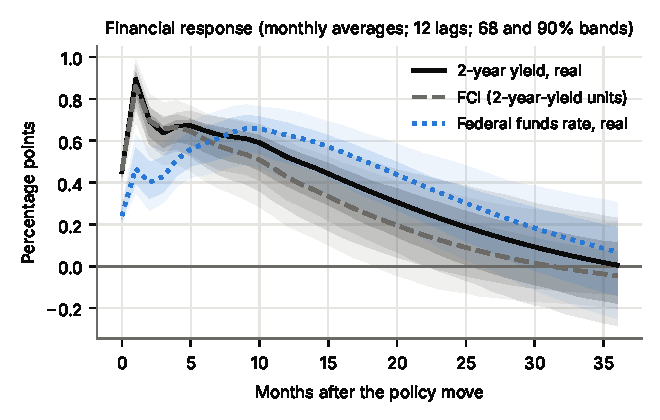
\includegraphics[width=0.62\textwidth]{../baseline_real/report/fig_financial.pdf}
\caption{Response of the Two-Year Yield, the FCI and the Funds Rate to a Policy Move}
\label{fig:financial}
\begin{flushleft}\footnotesize\textit{Notes:} Real versions, in percentage points (the FCI in two-year-yield units); the policy move raises the two-year yield 1 percentage point in the window. Monthly averages; 12 lags; 68 and 90 percent bands.\end{flushleft}
\end{figure}

\begin{figure}[tp]
\centering
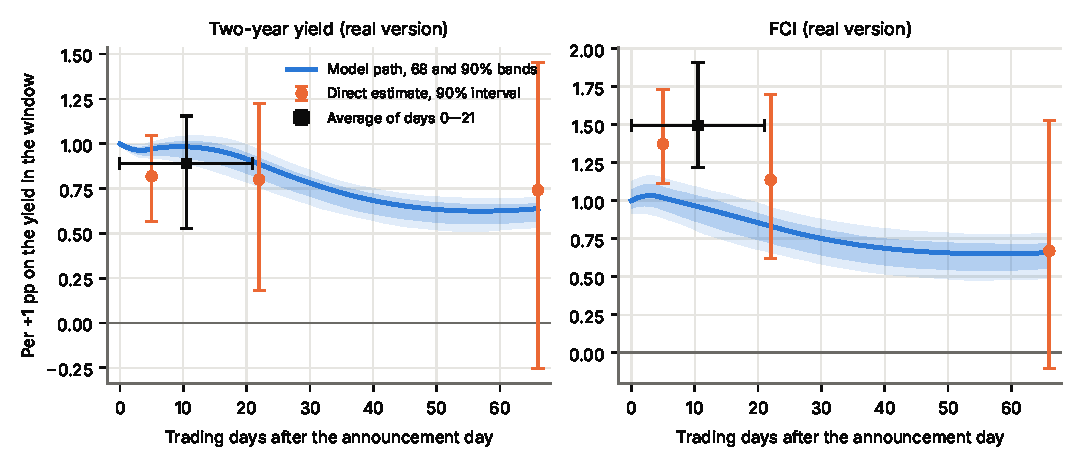
\includegraphics[width=\textwidth]{../baseline_real/report/fig_persist.pdf}
\caption{Financial Persistence: Direct Estimates and the Model}
\label{fig:persist}
\begin{flushleft}\footnotesize\textit{Notes:} Per +1 pp on the two-year yield in the window, real versions. Blue: the model's daily path after the announcement day (day 0), with 68 and 90 percent bands. Orange: direct estimates at 5, 22 and 66 trading days with 90 percent intervals. Black square: the average of days 0 to 21, with its interval; the horizontal bar shows the days averaged. The calendar-month averages of Figure~\ref{fig:financial} measure something different.\end{flushleft}
\end{figure}

\subsection{Monthly Benchmarks}\label{sec:monthlyvar}
Could a standard monthly model with the FCI added do the same job? A valid external instrument can recover the total response with the transmission channels unobserved, so a model with rates alone is not wrong by construction; the question is what works in these data. I estimate two monthly VARs with the real two-year yield, the FCI and the funds rate. A proxy VAR estimates the immediate effect of the surprise on every variable from monthly residuals and the instrument. A window-impact VAR takes the effect on the rates and the FCI from the windows, as the main model does, and sets the effect on unemployment and inflation to zero within the month; it has no daily block, so the timing of announcements within the month is lost.

\begin{table}[tp]\centering\small
\caption{Monthly VARs with the FCI and the Main Model (Real Two-Year Yield, FCI and Funds Rate; 12 Lags)}\label{tab:monthlycompact}
\resizebox{\ifdim\width>\textwidth\textwidth\else\width\fi}{!}{%
\begin{tabular}{lrrrr}\toprule & \multicolumn{2}{c}{Unemployment gap (pp)} & \multicolumn{2}{c}{Price level (\%)}\\ \cmidrule(lr){2-3}\cmidrule(lr){4-5} & 12 m & 24 m & 12 m & 24 m\\ \midrule
Proxy VAR & $-$0.08 & $-$0.11 & $-$0.47 & $-$0.65\\
 & {\scriptsize [$-$inf, inf]} & {\scriptsize [$-$inf, inf]} & {\scriptsize [$-$inf, inf]} & {\scriptsize [$-$inf, inf]}\\
Window-impact VAR & 0.17$^{*}$ & 0.16$^{*}$ & $-$0.14$^{*}$ & $-$0.23$^{*}$\\
 & {\scriptsize [0.05, 0.38]} & {\scriptsize [0.03, 0.51]} & {\scriptsize [$-$0.28, $-$0.02]} & {\scriptsize [$-$0.47, $-$0.04]}\\
Main model (daily block) & 0.33$^{*}$ & 0.40$^{*}$ & $-$0.27$^{*}$ & $-$0.49$^{*}$\\
 & {\scriptsize [0.16, 0.56]} & {\scriptsize [0.18, 0.78]} & {\scriptsize [$-$0.48, $-$0.13]} & {\scriptsize [$-$0.93, $-$0.17]}\\
\bottomrule\end{tabular}}
\begin{flushleft}\footnotesize\textit{Notes:} Per +1 pp on the two-year yield. $^{*}$: the 90\% interval excludes zero; intervals in brackets (Anderson--Rubin sets for the proxy VAR; bootstrap for the others). Monthly VARs use monthly averages; unit +1 pp on the two-year yield in the announcement window.\end{flushleft}
\end{table}


The window-impact VAR gives the signs of the main model at a smaller size (Table~\ref{tab:monthlycompact}): unemployment \bl{mo:real:yes:WE:u:12} percentage point higher after 12 months and the price level \blabs{mo:real:yes:WE:P:24} percent lower after 24, about half the main model's \bl{real:yes:u:12} and \blabs{real:yes:P:24}; from 1973 it gives \bl{mo73:real:yes:WE:u:12} and \blabs{mo73:real:yes:WE:P:24}. The proxy VAR has wide sets, because the surprise is a weak instrument for monthly residuals (first-stage $F$ of \bl{mo:real:yes:F} from 1996 and \bl{mo73:real:yes:F} from 1973). The smaller size is what monthly averaging does. A window move of 1 percentage point raises the month's average yield by only \bl{mo:win}, and a monthly VAR cannot reproduce the rest of the movement, which arrives the next month. A simulation with the baseline model as the true process confirms this: the window-impact VAR recovers about half the true unemployment response at 12 months (median \bl{sim:window:u12:med} against \bl{sim:window:u12:truth}) with a narrow range, the proxy VAR with the FCI is centred below the truth with a range that runs from \bl{sim:proxy_fci:u12:lo} to \bl{sim:proxy_fci:u12:hi}, and the proxy VAR without the FCI has a median of the wrong sign (\bl{sim:proxy_nofci:u12:med}; Appendix Table~\ref{tab:proxysim}). The main model estimated without the FCI on the same samples also has a median of the wrong sign (\bl{sim:main_nofci:u12:med}). The data estimates are ordinary draws from these distributions. Tracking the daily path of the financial movement, as the main model does, is what recovers the full response \citep{jacobson2026}.

A direct projection of each outcome on the surprise imposes no channel at all (Appendix~\ref{app:direct}). With lags of unemployment and inflation as the only controls it gives large wrong-signed estimates: unemployment \bl{dp:m:u:12} percentage point after 12 months. Adding lags of the rates and the FCI shrinks the estimates toward zero (\bl{dp:f:u:12}), and no interval then excludes zero. The surprise by itself does not pin down the macroeconomic response. A model of financial propagation, or at least the monthly dynamics of a VAR, is needed for an informative estimate.

\subsection{Credit Spreads}\label{sec:credit}
Credit is the most important channel the baseline leaves out \citep{gertler2015,gilchrist2012,caldara2019}. If a credit premium that responds to policy carried part of what the FCI carries, the FCI would take credit for effects that belong to credit. I add the Baa corporate spread over the 10-year Treasury yield to the daily block, next to the rates and, in the full model, the FCI, and estimate the model with and without the FCI (Table~\ref{tab:credit}). The spread has no intraday series, so its impact is its change on the announcement day, \bl{rv:cr:baaimp} percentage point per percentage point on the yield: the 10-year yield rises on the day by more than the Baa yield, which partly reflects the slow adjustment of quoted corporate yields. As a check on activity, I add industrial production to the monthly block in the same way.

\begin{table}[tp]\centering\small
\caption{Credit, Activity and the Effect of Adding the FCI (Real Rates; 24 Months)}\label{tab:credit}
\resizebox{\ifdim\width>\textwidth\textwidth\else\width\fi}{!}{%
\begin{tabular}{lcccc}\toprule & \multicolumn{2}{c}{Unemployment gap (pp)} & \multicolumn{2}{c}{Effect of adding the FCI} \\ \cmidrule(lr){2-3}\cmidrule(lr){4-5}
 & Rates alone & Rates and FCI & Unemployment gap & Price level (\%)\\ \midrule
Baseline & $-$0.33$^{*}$ & 0.40$^{*}$ & 0.73$^{*}$ & $-$0.43$^{*}$\\
 & {\scriptsize [$-$0.60, $-$0.08]} & {\scriptsize [0.13, 0.68]} & {\scriptsize [0.37, 1.04]} & {\scriptsize [$-$0.82, $-$0.09]}\\
Baa spread in the daily block & $-$0.22 & 0.27 & 0.49$^{*}$ & $-$0.50$^{*}$\\
 & {\scriptsize [$-$0.58, 0.12]} & {\scriptsize [$-$0.05, 0.55]} & {\scriptsize [0.19, 0.77]} & {\scriptsize [$-$0.80, $-$0.15]}\\
Industrial production in the monthly block & $-$0.07 & 0.52$^{*}$ & 0.59$^{*}$ & $-$0.60$^{*}$\\
 & {\scriptsize [$-$0.38, 0.13]} & {\scriptsize [0.22, 0.86]} & {\scriptsize [0.31, 0.96]} & {\scriptsize [$-$1.01, $-$0.29]}\\
\bottomrule\end{tabular}}
\begin{flushleft}\footnotesize\textit{Notes:} Per +1 pp on the two-year yield in the announcement window; real two-year yield and funds rate, 12 lags, monthly equations from 1996, March--December 2020 dropped. Baa spread: Moody's Baa yield less the 10-year Treasury yield, in the daily block next to the rates (and the FCI); its impact is its announcement-day change on the surprise, because it has no intraday series; months before the daily data (1986) use the monthly series. Industrial production: $100\ln$ of the index, a third monthly variable, set like unemployment and inflation before markets within the month. Effect of adding the FCI: the response with the FCI less the response with the same variables without it. All cases use the same bootstrap draws, so the effects are paired; 90 percent intervals in brackets; $^{*}$: the 90 percent interval excludes zero.\end{flushleft}
\end{table}


Neither changes what the FCI adds. With the spread, adding the FCI raises the two-year unemployment response by \bl{rv:cr:baa:eff:u} percentage point and lowers the price level by \blabs{rv:cr:baa:eff:P} percent, against \bl{rv:cr:base:eff:u} and \blabs{rv:cr:base:eff:P} in the baseline; with industrial production, by \bl{rv:cr:ip:eff:u} and \blabs{rv:cr:ip:eff:P}. None of these effects differs significantly from the baseline's. Without the FCI, unemployment still falls after a tightening in both cases (\bl{rv:cr:baa:0:u} and \bl{rv:cr:ip:0:u} percentage point after two years). The spread itself moves little after a tightening once the FCI is in the model: after 12 months it is \bl{rv:cr:baa12} percentage point, with an interval that includes zero.

\subsection{Temporal Aggregation and Financial Conditions}\label{sec:timingtest}
\citet{jacobson2026} show that averaging daily data into months biases the estimated effects of policy, because a surprise late in a month barely affects that month's average while one early in the month affects most of it. My model differs from the window-impact monthly VAR of Section~\ref{sec:monthlyvar} in two ways: it tracks when in the month each announcement falls, and it estimates the dynamics of the rates and the FCI on daily data. Comparing the two, with and without the FCI, measures the two differences together (Table~\ref{tab:timing2}).

\begin{table}[tp]\centering\small
\caption{Two Corrections: Announcement Timing and Financial Conditions (24 Months; 12 Lags)}\label{tab:timing2}
\resizebox{\ifdim\width>\textwidth\textwidth\else\width\fi}{!}{%
\begin{tabular}{llcccc}\toprule & & \multicolumn{2}{c}{Yield alone} & \multicolumn{2}{c}{Yield and FCI}\\ \cmidrule(lr){3-4}\cmidrule(lr){5-6}
Yield & Response & Monthly VAR & Daily block & Monthly VAR & Daily block\\ \midrule
Nominal & Unemployment gap (pp) & $-$0.35$^{*}$ & $-$0.35$^{**}$ & 0.08 & 0.40$^{**}$\\
 & Price level (\%) & 0.10 & $-$0.05 & $-$0.13 & $-$0.49$^{*}$\\\addlinespace
Real & Unemployment gap (pp) & $-$0.19 & $-$0.33$^{**}$ & 0.16 & 0.40$^{**}$\\
 & Price level (\%) & $-$0.05 & $-$0.06 & $-$0.23 & $-$0.49$^{**}$\\
\bottomrule\end{tabular}}
\begin{flushleft}\footnotesize\textit{Notes:} Per +1 pp on the two-year yield in the announcement window, 1996--2026. Monthly VAR: the window-impact monthly VAR of Section~\ref{sec:monthlyvar}, which takes the impact from the windows and treats every announcement as if it fell at the start of its month (end-of-month series). Daily block: the main model, which tracks when in the month each announcement falls. $^{**}$ and $^{*}$: the 95 and 90 percent intervals exclude zero.\end{flushleft}
\end{table}


With the rates alone, neither model gives a rise in unemployment, whether the timing is tracked or not. Adding the FCI raises the unemployment response after 24 months in both versions, by \bl{rv:tm:nom:u:fci} and \bl{rv:tm:real:u:fci} percentage point on average across the two models for nominal and real rates. The daily block adds \bl{rv:tm:nom:u:timefci} and \bl{rv:tm:real:u:timefci} once the FCI is in the model, and \bl{rv:tm:nom:u:timeno} and \bl{rv:tm:real:u:timeno} without it. Calendar position accounts for none of this: with the main model's estimated equations, placing every announcement on the first day of its month or at mid-month changes the real responses by at most \bl{rv:tmo:max}. The gain comes from the daily dynamics of the rates and the FCI after an announcement, and it is largest when the financial movement is large. Omitted financial channels and temporal aggregation are thus two sources of the puzzle, and the financial channel is the larger one. \citet{jacobson2026} correct the second with a daily price index; this paper corrects the first with standard monthly data on core prices and unemployment.

\FloatBarrier
% ============================================================
\section{Robustness}\label{sec:rob}
A result about the transmission of monetary policy can rest on one sample, one set of variables, one surprise series or one lag length. I vary each in turn, changing one feature of the baseline and keeping the rest (Table~\ref{tab:robsummary}). Each test is run from both starting dates, except a later start for the monthly equations. The table reports the responses after 12 months, where both are well measured in both samples, for real and nominal rates; the appendix gives 12, 24 and 36 months for both versions and every test.

\begin{table}[tp]\centering\small
\caption{Robustness: Responses at 12 Months}\label{tab:robsummary}
\resizebox{\ifdim\width>\textwidth\textwidth\else\width\fi}{!}{%
\begin{tabular}{lcccc}\toprule & \multicolumn{2}{c}{Monthly equations from 1996} & \multicolumn{2}{c}{Monthly equations from 1973}\\ \cmidrule(lr){2-3}\cmidrule(lr){4-5} & Unemployment gap & Price level & Unemployment gap & Price level\\ \midrule
\multicolumn{5}{l}{\textit{Real 2-year yield, funds rate and FCI}}\\
Baseline & 0.33$^{**}$ & $-$0.27$^{**}$ & 0.19$^{**}$ & $-$0.28$^{**}$\\
 & {\scriptsize [0.13, 0.50]} & {\scriptsize [$-$0.44, $-$0.08]} & {\scriptsize [0.06, 0.31]} & {\scriptsize [$-$0.38, $-$0.14]}\\
2020 left in & 0.24 & $-$0.30$^{**}$ & 0.02 & $-$0.21$^{**}$\\
 & {\scriptsize [$-$0.25, 0.62]} & {\scriptsize [$-$0.50, $-$0.10]} & {\scriptsize [$-$0.16, 0.22]} & {\scriptsize [$-$0.32, $-$0.06]}\\
Excess bond premium and industrial production added & 0.24$^{*}$ & $-$0.30$^{**}$ & 0.13$^{**}$ & $-$0.17$^{**}$\\
 & {\scriptsize [0.02, 0.41]} & {\scriptsize [$-$0.45, $-$0.09]} & {\scriptsize [0.02, 0.26]} & {\scriptsize [$-$0.25, $-$0.04]}\\
Bauer--Swanson surprise & 0.37$^{**}$ & $-$0.29$^{**}$ & 0.22$^{**}$ & $-$0.28$^{**}$\\
 & {\scriptsize [0.16, 0.55]} & {\scriptsize [$-$0.47, $-$0.10]} & {\scriptsize [0.09, 0.35]} & {\scriptsize [$-$0.38, $-$0.13]}\\
6 lags & 0.26$^{**}$ & $-$0.19 & 0.11 & $-$0.18$^{**}$\\
 & {\scriptsize [0.08, 0.40]} & {\scriptsize [$-$0.36, 0.01]} & {\scriptsize [$-$0.01, 0.21]} & {\scriptsize [$-$0.27, $-$0.02]}\\
Without the funds rate & 0.17$^{*}$ & $-$0.22$^{**}$ & 0.25$^{**}$ & $-$0.24$^{**}$\\
 & {\scriptsize [0.01, 0.35]} & {\scriptsize [$-$0.38, $-$0.05]} & {\scriptsize [0.11, 0.35]} & {\scriptsize [$-$0.33, $-$0.11]}\\
Monthly equations from 1985 & 0.12 & $-$0.07 &  & \\
 & {\scriptsize [$-$0.06, 0.23]} & {\scriptsize [$-$0.19, 0.11]} &  & \\
\addlinespace\multicolumn{5}{l}{\textit{Nominal 2-year yield, funds rate and FCI}}\\
Baseline & 0.27$^{*}$ & $-$0.18 & 0.13 & $-$0.08\\
 & {\scriptsize [0.03, 0.47]} & {\scriptsize [$-$0.36, 0.06]} & {\scriptsize [$-$0.01, 0.26]} & {\scriptsize [$-$0.19, 0.05]}\\
2020 left in & 0.35 & $-$0.18 & $-$0.13 & 0.02\\
 & {\scriptsize [$-$0.13, 0.75]} & {\scriptsize [$-$0.40, 0.05]} & {\scriptsize [$-$0.36, 0.06]} & {\scriptsize [$-$0.09, 0.19]}\\
Excess bond premium and industrial production added & 0.39$^{**}$ & $-$0.31$^{**}$ & 0.17$^{**}$ & $-$0.03\\
 & {\scriptsize [0.11, 0.55]} & {\scriptsize [$-$0.48, $-$0.09]} & {\scriptsize [0.06, 0.28]} & {\scriptsize [$-$0.13, 0.10]}\\
Bauer--Swanson surprise & 0.32$^{**}$ & $-$0.19 & 0.17$^{**}$ & $-$0.08\\
 & {\scriptsize [0.05, 0.52]} & {\scriptsize [$-$0.39, 0.06]} & {\scriptsize [0.02, 0.30]} & {\scriptsize [$-$0.19, 0.06]}\\
6 lags & 0.06 & $-$0.17 & 0.04 & $-$0.03\\
 & {\scriptsize [$-$0.14, 0.24]} & {\scriptsize [$-$0.36, 0.05]} & {\scriptsize [$-$0.10, 0.14]} & {\scriptsize [$-$0.13, 0.12]}\\
Without the funds rate & 0.13 & $-$0.14 & 0.29$^{**}$ & $-$0.01\\
 & {\scriptsize [$-$0.04, 0.36]} & {\scriptsize [$-$0.33, 0.07]} & {\scriptsize [0.13, 0.41]} & {\scriptsize [$-$0.13, 0.12]}\\
Monthly equations from 1985 & 0.04 & 0.02 &  & \\
 & {\scriptsize [$-$0.12, 0.16]} & {\scriptsize [$-$0.08, 0.17]} &  & \\
\bottomrule\end{tabular}}
\begin{flushleft}\footnotesize\textit{Notes:} Two-year yield, federal funds rate and FCI in the stated version; responses 12 months after a policy move that raises the two-year yield 1 percentage point in the announcement window; unemployment gap in percentage points, price level in percent; 12 lags unless stated; March--December 2020 dropped unless stated. The 1985 start has monthly equations from January 1985 (1996 columns). $^{**}$ and $^{*}$: the 95\% and 90\% bootstrap intervals exclude zero; 90\% intervals in brackets. Full results at 12, 24 and 36 months for both versions are in the appendix.\end{flushleft}
\end{table}


The real responses are uniform in sign and close in size. In every test and both samples, a tightening raises unemployment and lowers the price level after a year. From 1996 the unemployment responses lie between \bl{rob:real:s85:u} and \bl{rob:real:bs:u} percentage point around the baseline's \bl{rob:real:base:u}, and the price responses between \bl{rob:real:s85:P} and \bl{rob:real:ip:P} percent around \bl{rob:real:base:P}. From 1973 the price responses lie between \bl{rob:real:L673:P} and \bl{rob:real:bs73:P} percent around the baseline's \bl{rob:real:base73:P}. Two tests give clearly smaller responses: monthly equations that start in 1985, and, for unemployment, keeping 2020 in the sample from 1973. The nominal version is close to the real one since 1996 and weaker from 1973, as in the baselines.

\subsection{The Sample}\label{sec:recent}
The sample since 1996 is short, it contains the pandemic, when unemployment moved by more than in any other period, and it ends with the largest tightening in the sample. Keeping March to December 2020 in the estimation leaves the price responses in place (\bl{rob:real:t2020:P} percent after a year from 1996 and \bl{rob:real:t202073:P} from 1973) and lowers the unemployment response, to \bl{rob:real:t2020:u} percentage point from 1996 and \bl{rob:real:t202073:u} from 1973, with wider intervals: the pandemic months dominate the unemployment equation when they are in it.

Starting the monthly equations in January 1985, after the disinflation of the early 1980s, gives the smallest responses: \bl{rob:real:s85:u} percentage point for unemployment and \bl{rob:real:s85:P} percent for the price level after a year. That sample loses the large movements of inflation and rates before 1985 and adds to the sample since 1996 only the decade of the Great Moderation, when inflation and unemployment moved little. The two baselines bracket it: the sample from 1973 has the variation in inflation, and the sample since 1996 has the announcements and the daily data on which the financial block is estimated.

Ending all equations in December 2019 removes the post-pandemic inflation. From 1996 the price level then does not fall (\bl{sm:end96:P:24} percent after two years, against \bl{sm:base96:P:24}), while unemployment still rises; from 1973 it falls \bl{sm:end73:P:24:abs} percent, close to the baseline (Appendix Table~\ref{tab:mainA}). Core inflation varied little before 2020 (a standard deviation of \bl{sm:pi:sd:9619} percentage points for 1996--2019, against \bl{sm:pi:sd:2026} for 2020--26 and \bl{sm:pi:sd:7319} for 1973--2019), so the short sample has little information on how inflation responds to financial conditions, and the later years and the earlier decades supply it.

\subsection{Further Variables}\label{sec:extensions}
Adding industrial production as a further monthly variable leaves the responses close to the baseline in both samples (\bl{rob:real:ip:u} and \bl{rob:real:ip:P} after a year from 1996, \bl{rob:real:ip73:u} and \bl{rob:real:ip73:P} from 1973). Removing the funds rate, so that the two-year yield is the only rate, gives smaller responses from 1996 (\bl{rob:real:noff:u} and \bl{rob:real:noff:P}) and similar ones from 1973 (\bl{rob:real:noff73:u} and \bl{rob:real:noff73:P}). The funds rate adds most where the lower bound binds most often.

\subsection{The Index Weights and Restriction}\label{sec:restriction}
With the weights of the Goldman Sachs index, the index most followed in markets, the responses are nearly the same: \bl{rob:real:gs:u} percentage point for unemployment and \bl{rob:real:gs:P} percent for the price level after a year from 1996, against \bl{rob:real:base:u} and \bl{rob:real:base:P} (Table~\ref{tab:robsummary}). The FCI enters the monthly equations as one variable, so its three asset prices act on unemployment and inflation in proportion to their weights. Replacing the index with its three weighted components, each with its own coefficients, tests that restriction (Table~\ref{tab:robsummary}, last row of the real block). The unemployment response is unchanged: \bl{cm::F:u:24} percentage point after two years from 1996 with the components free, against \bl{cm::R:u:24} with the index built from them. In the first year the price level falls by slightly less, and the differences are not significant (\bl{cm::F:P:12:abs} against \bl{cm::R:P:12:abs} percent from 1996, \bl{cm:73:F:P:12:abs} against \bl{cm:73:R:P:12:abs} from 1973). After two years it falls by less (\bl{cm::F:P:24:abs} against \bl{cm::R:P:24:abs} percent from 1996, \bl{cm:73:F:P:24:abs} against \bl{cm:73:R:P:24:abs} from 1973). Equal coefficients on the three components are rejected at the 5 percent level in the inflation equation in both samples and in the unemployment equation in neither. The Bayesian information criterion favours the restriction in every equation.

\subsection{The Surprise and Lag Length}\label{sec:surprise}
An announcement can reveal the Fed's view of the economy as well as a change in policy, and part of each surprise can be predicted from public data. The orthogonalized surprise of \citet{bauer2023}, which removes the predictable part and is available through 2019 (\bl{ev:bs} announcements), gives responses at least as large as the baseline's in both samples (\bl{rob:real:bs:u} and \bl{rob:real:bs:P} after a year from 1996); the orthogonalized surprise changes only the initial direction of the shock, and the daily and monthly equations are the baseline's. The baseline uses 12 monthly lags, fixed in advance. With 6 lags the unemployment response from 1996 is close to the baseline (\bl{lag:real:u24:6} percentage point after two years, against \bl{lag:real:u24:12}) and the price fall is about a fifth smaller; from 1973 both are smaller (Appendix~\ref{app:lags}).

\FloatBarrier
% ============================================================
\section{How Much Do Surprises in the Policy Direction Explain?}\label{sec:shares}
The responses measure what a policy move does. A different question is how much of the movement in unemployment and inflation surprises of this kind account for. I answer it with a narrow measure and a broad one, using the two baselines to propagate them.

The narrow measure is the announcement surprises. The 252 window surprises, carried through the model, account for \bl{dc:yes:1996:meas:u:24} percent of the variance of unemployment and \bl{dc:yes:1996:meas:pi:24} percent of the variance of core inflation over two-year horizons (Table~\ref{tab:decompshares}). The surprises are small: their standard deviation is \bl{sd:ns:bp} basis points, and most announcements contain little news about the path of rates. They identify the effect of policy well and explain almost none of the fluctuations.

The broad measure uses every day. Let $\varepsilon_d$ be the innovations of the daily block on day $d$ (the two-year yield, the FCI and the funds rate), with covariance $\Omega$, and $b$ the movement of the three on an announcement (equation~\eqref{eq:impact}). Each day's innovations split into a surprise in the policy direction and the rest:
\begin{equation}
\varepsilon_d = b\,\hat s_d + r_d, \qquad \hat s_d = \frac{b'\Omega^{-1}\varepsilon_d}{b'\Omega^{-1}b}. \label{eq:pdsplit}
\end{equation}
Weighting by $\Omega^{-1}$ makes $\hat s_d$ and $r_d$ uncorrelated, so the split is unique given $b$ and $\Omega$. The surprise $\hat s_d$ measures how far the day's innovations move in the proportion of an announcement; it does not identify their source. On announcement days it has a correlation of \bl{dc:ann:corr} with the announcement surprise. On other days it includes news about the economy, earnings or risk appetite, to the extent that such news moves the rates and the FCI in that proportion. Its contribution to unemployment and inflation uses the model's response to $b$: the main assumption of Section~\ref{sec:timing}, that the economy responds to the movement in the same way whatever caused it. Before May 1990 there are no daily data, and the surprises are the monthly analogue of equation~\eqref{eq:pdsplit}, $\hat e_t = b'S^{-1}u_t / b'S^{-1}b$, from the innovations $u_t$ of a monthly VAR with covariance $S$, rescaled to the monthly size of the daily surprises after 1990. The figures for 1974--1989 are therefore a backcast; without the rescaling their shares are \bl{dc:yes:1973:pd74:u:24:infer_unscaled} and \bl{dc:yes:1973:pd74:pi:24:infer_unscaled} percent in the model from 1973.

Surprises in the policy direction account for a modest share of the variance of unemployment and inflation. Propagated through the model from 1973, they explain \bl{dc:yes:1973:pd90:u:24} percent of the two-year variance of unemployment and \bl{dc:yes:1973:pd90:pi:24} percent of that of core inflation since 1990, and \bl{dc:yes:1973:pd74:u:24} and \bl{dc:yes:1973:pd74:pi:24} percent over 1974--1989. The model from 1996, with its larger unemployment response, gives \bl{dc:yes:1996:pd90:u:24} and \bl{dc:yes:1996:pd90:pi:24} percent since 1990. Nearly all of it comes from days without an announcement. The shares are ratios of variances and need not add up: the contributions of announcement days and other days are correlated, so the share of other days alone can exceed the total. The same surprises account for about a quarter of the variance of the two-year yield (\bl{dc:yes:1973:pd90:pol:24} percent); the rest of its movement comes with financial conditions in other proportions.

\begin{figure}[tp]
\centering
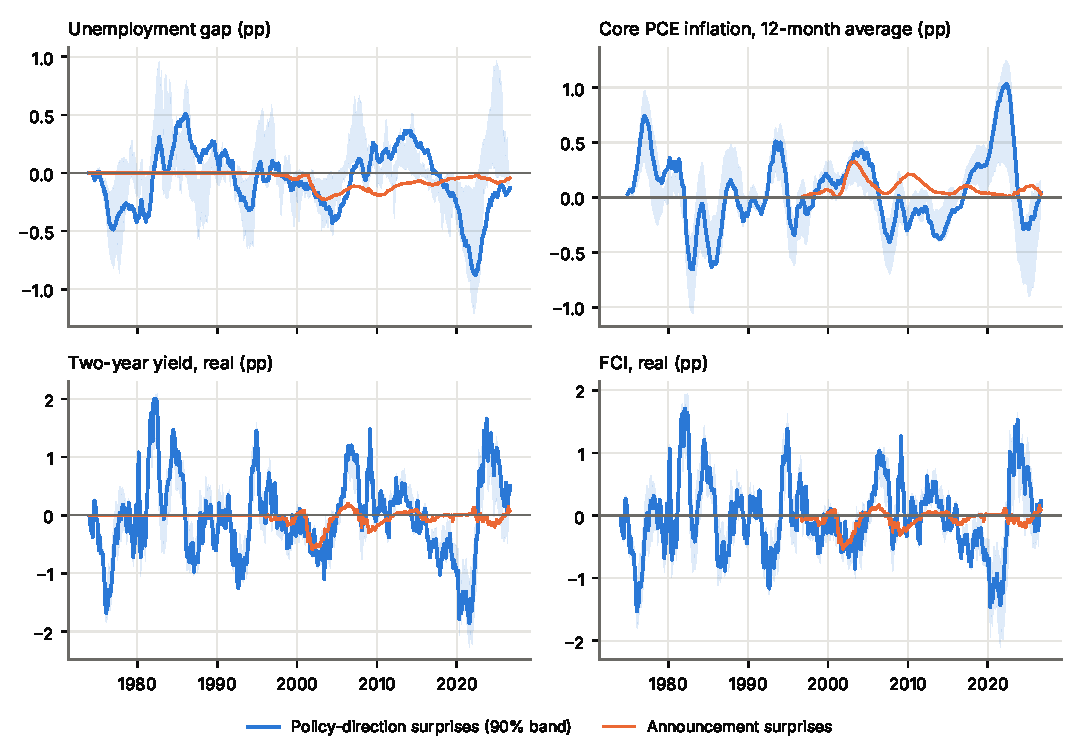
\includegraphics[width=\textwidth]{../baseline_real/report/fig_decomp_hd.pdf}
\caption{Contributions of Surprises in the Policy Direction, 1974--2026}
\label{fig:decomphd}
\begin{flushleft}\footnotesize\textit{Notes:} Historical contributions of policy-direction surprises (equation~\eqref{eq:pdsplit}; before May 1990 the monthly backcast) to the unemployment gap, core PCE inflation (12-month average), the real two-year yield and the real FCI, propagated through the real model with monthly equations from 1973 (12 lags, March--December 2020 dropped from estimation; the 2020 surprises are decomposed with the estimated coefficients). Orange: the contributions of the announcement surprises. Band: 90 percent interval from the bootstrap draws of the model's responses.\end{flushleft}
\end{figure}

\begin{table}[tp]\centering\small
\caption{How Much Policy Shocks Explain: Variance Shares at 24 Months}\label{tab:decompshares}
\resizebox{\ifdim\width>\textwidth\textwidth\else\width\fi}{!}{%
\begin{tabular}{lcccc}\toprule & \multicolumn{2}{c}{Model from 1996} & \multicolumn{2}{c}{Model from 1973}\\ \cmidrule(lr){2-3}\cmidrule(lr){4-5} Shocks & Unemployment gap & Core inflation & Unemployment gap & Core inflation\\ \midrule
Measured window surprises, 1996--2026 & 0.7 & 0.3 & 0.2 & 0.2\\
 & {\scriptsize [0.1, 1.6]} & {\scriptsize [0.1, 0.6]} & {\scriptsize [0.0, 0.5]} & {\scriptsize [0.1, 0.4]}\\
Policy-direction shocks, 1990--2026 & 11.6 & 5.7 & 3.2 & 4.1\\
 & {\scriptsize [2.1, 29.7]} & {\scriptsize [2.5, 11.6]} & {\scriptsize [0.5, 9.1]} & {\scriptsize [1.4, 7.2]}\\
\quad of which on days without an announcement & 12.6 & 5.7 & 3.5 & 4.5\\
 & {\scriptsize [2.2, 32.1]} & {\scriptsize [2.4, 12.1]} & {\scriptsize [0.5, 9.8]} & {\scriptsize [1.4, 7.8]}\\
Policy-direction shocks, 1974--1989 & 12.2 & 4.3 & 3.4 & 3.6\\
 & {\scriptsize [2.4, 31.0]} & {\scriptsize [2.6, 10.5]} & {\scriptsize [0.5, 9.6]} & {\scriptsize [1.3, 6.6]}\\
\bottomrule\end{tabular}}
\begin{flushleft}\footnotesize\textit{Notes:} Percent of the 24-month forecast-error variance (monthly VAR in monthly averages from 1973, 12 lags) accounted for by the contributions of the shocks of the last 24 months, propagated through the real model with the FCI and the funds rate (12 lags, March--December 2020 dropped) with monthly equations from 1996 or from 1973; shares over the stated period, March--December 2020 excluded. Measured window surprises: the 252 announcements. Policy-direction shocks: the daily movement of the two-year yield and the FCI in the direction of the window response, recovered from the daily block on every day from 1990; before 1990 from the monthly VAR, scaled to the daily shocks' size. Brackets: 90\% bootstrap bands of Note B's responses.\end{flushleft}
\end{table}


The history is best read in changes, because the effects build with lags (Figure~\ref{fig:decomphd}). Each line is the cumulative contribution of past surprises, so a change in the direction of policy appears first as the fading of an earlier contribution and only later as a contribution of the opposite sign. Through the first half of 1981 the surprises had added about \bl{dc:hy:pi:1981H1:r1} percentage point to core inflation and held unemployment about \bl{dc:hy:u:1981H1:r1} point lower. The Volcker tightening reversed this. Between the first halves of 1981 and 1982 their contribution to the real two-year yield rose by \bl{dc:hy:d:vpol} percentage points and their contribution to inflation fell by \bl{dc:hy:d:vpi}, to \bl{dc:hy:pi:1982H1}. Unemployment followed with a lag: its contribution turned positive in 1982 and reached about \bl{dc:hy:u:1985H2:r1} point by the end of 1985. The 2020s show the same sequence. From 2019 to late 2021 the contribution to the yield fell by \bl{dc:hy:d:cpol1} percentage points and the contribution to inflation rose to about \bl{dc:hy:pi:2021H2:r1} point; over 2021--22 it averaged \bl{dc:hist:pi2122} (\bl{dc:hist:pi2122:absorb} with the surprises of March to December 2020 set to zero, and \bl{dc:hist:pi2122:meas} from the announcement surprises alone). The tightening of 2022 raised the contribution to the yield by \bl{dc:hy:d:cpol2} percentage points by the end of 2023 and turned the contribution to inflation negative. The contribution to unemployment rose by \bl{dc:hy:d:cu} point from early 2022 to 2025, as the earlier easing faded. The announcement surprises, in orange, are a small part of each episode. The surprises come from the daily block rather than from a monthly VAR because a surprise concentrated on one day is weakly recovered from the innovations of its month: those innovations explain \bl{dc:diag:real:yes:1973:r2} percent of the variance of the month's summed surprises in the model from 1973.\footnote{Appendix~\ref{app:relation} reports this diagnostic for each version and sample. Appendix Table~\ref{tab:decompfull} gives the shares for every source and horizon, with the 2020 surprises absorbed by the month dummies and with the backcast before 1990 unscaled.}

\FloatBarrier
% ============================================================
\section{Slow-Moving Rates and Financial Conditions}\label{sec:slow}
Real interest rates and financial conditions moved slowly over the sample. The neutral rate $\rs$, the real rate that neither speeds up nor slows down the economy, fell from the 1990s to the 2010s \citep{laubach2003,holston2017,holston2023,hamilton2016,bauer2020,kiley2020}, and real yields and stock valuations moved with it while activity did not. A model that links the level of rates to activity can partly pick up these opposite trends. How to separate the slow movement of rates from the stance of policy is a large question, mostly beyond this paper. This section shows how much of the variation in the data is slow and what two common treatments of it do to the results.

\begin{table}[tp]\centering\scriptsize\setlength{\tabcolsep}{3pt}
\caption{Variance Fitted by a Spline Trend}\label{tab:slowshares}
\resizebox{\ifdim\width>\textwidth\textwidth\else\width\fi}{!}{%
\begin{tabular}{lrrrrrrrrrr}\toprule & \multicolumn{5}{c}{Monthly equations from 1996} & \multicolumn{5}{c}{Monthly equations from 1973}\\ \cmidrule(lr){2-6}\cmidrule(lr){7-11}
Version & FCI & Two-year yield & Federal funds rate & Unemployment gap & Core PCE inflation & FCI & Two-year yield & Federal funds rate & Unemployment gap & Core PCE inflation\\ \midrule
Nominal & 42 & 69 & 61 & 55 & 20 & 94 & 85 & 75 & 37 & 63\\
Real & 32 & 63 & 51 & 55 & 20 & 92 & 75 & 58 & 37 & 63\\
Relative to $r^*$ & 56 & 45 & 38 & 55 & 20 & 79 & 56 & 40 & 37 & 63\\
\bottomrule\end{tabular}}
\begin{flushleft}\footnotesize\textit{Notes:} Percent of the variance of each monthly series (monthly averages over the estimation months of the model, 12 lags, March--December 2020 dropped) fitted by a natural cubic spline in time with knots at the first and last estimation months and at the NBER business-cycle peaks inside the sample. The unemployment gap and inflation do not depend on the version. $r^*$-gap: Laubach--Williams $r^*$.\end{flushleft}
\end{table}


Much of the variation is slow (Table~\ref{tab:slowshares}). A natural cubic spline in time, with knots at the first and last months of the sample and at the business-cycle peaks between them, fits \bl{slow:real73:idx} percent of the variance of the real FCI and \bl{slow:real73:pol} percent of that of the real two-year yield in the sample from 1973, and \bl{slow:real:idx} and \bl{slow:real:pol} percent since 1996. It also fits \bl{slow:real:u} percent of the variance of the unemployment gap since 1996, because the gap moved over long cycles in those years. Measuring rates and the index relative to $\rs$ removes part of the slow movement over five decades: a linear trend explains \bl{tr:r:r2} percent of the variance of the real FCI since 1973 and \bl{tr:s:r2} percent of the version relative to $\rs$, and the spline fits \bl{slow:rstar73:idx} percent of the latter. Since 1996 the picture is different: the spline fits more of the version relative to $\rs$ (\bl{slow:rstar:idx} percent) than of the real version.

The version relative to $\rs$ measures the two-year yield and the funds rate less expected inflation and the one-sided Laubach--Williams estimate of $\rs$ \citep{laubach2003}. Stocks enter through the earnings yield relative to $\rs$, rescaled to the units of log CAPE, so a fall in $\rs$ of 1 percentage point lowers the neutral level of the index by \bl{rv:kap} units; in this sense the index relative to $\rs$ is a reduced-form gap to a neutral level of financial conditions, as in \citet{caballero2026}. The spline instead removes a flexible time trend from every monthly equation and leaves the rates and the index in real terms.

\begin{table}[tp]\centering\scriptsize\setlength{\tabcolsep}{2.5pt}
\caption{Slow-Moving Rates: The $r^*$-Gap Step and a Spline Trend}\label{tab:slowresp}
\resizebox{\ifdim\width>\textwidth\textwidth\else\width\fi}{!}{%
\begin{tabular}{lrrrrrrrr}\toprule & \multicolumn{4}{c}{Nominal} & \multicolumn{4}{c}{Real (the $r^*$-gap row: $r^*$-gap)}\\ \cmidrule(lr){2-5}\cmidrule(lr){6-9} & \multicolumn{2}{c}{Unemployment gap} & \multicolumn{2}{c}{Price level} & \multicolumn{2}{c}{Unemployment gap} & \multicolumn{2}{c}{Price level}\\ & 12 m & 24 m & 12 m & 24 m & 12 m & 24 m & 12 m & 24 m\\ \midrule
\multicolumn{9}{l}{\textit{Monthly equations from 1996}}\\
Baseline (no trend) & 0.27$^{*}$ & 0.40$^{**}$ & $-$0.18 & $-$0.49$^{*}$ & 0.33$^{**}$ & 0.40$^{**}$ & $-$0.27$^{**}$ & $-$0.49$^{**}$\\
 & {\tiny [0.03, 0.47]} & {\tiny [0.09, 0.65]} & {\tiny [$-$0.36, 0.06]} & {\tiny [$-$0.80, $-$0.03]} & {\tiny [0.13, 0.50]} & {\tiny [0.13, 0.68]} & {\tiny [$-$0.44, $-$0.08]} & {\tiny [$-$0.86, $-$0.12]}\\
Spline trend & 0.18 & 0.34 & $-$0.08 & $-$0.24 & 0.25 & 0.32 & $-$0.15 & $-$0.20\\
 & {\tiny [$-$0.10, 0.35]} & {\tiny [$-$0.10, 0.68]} & {\tiny [$-$0.27, 0.19]} & {\tiny [$-$0.70, 0.25]} & {\tiny [$-$0.03, 0.38]} & {\tiny [$-$0.12, 0.53]} & {\tiny [$-$0.32, 0.09]} & {\tiny [$-$0.64, 0.23]}\\
$r^*$-gap (LW) & \multicolumn{4}{c}{} & 0.43$^{**}$ & 0.49$^{**}$ & $-$0.42$^{**}$ & $-$0.81$^{**}$\\
 & \multicolumn{4}{c}{} & {\tiny [0.17, 0.61]} & {\tiny [0.12, 0.81]} & {\tiny [$-$0.58, $-$0.19]} & {\tiny [$-$1.19, $-$0.34]}\\
\addlinespace
\multicolumn{9}{l}{\textit{Monthly equations from 1973}}\\
Baseline (no trend) & 0.13 & 0.12 & $-$0.08 & $-$0.22 & 0.19$^{**}$ & 0.19 & $-$0.28$^{**}$ & $-$0.56$^{**}$\\
 & {\tiny [$-$0.01, 0.26]} & {\tiny [$-$0.07, 0.27]} & {\tiny [$-$0.19, 0.05]} & {\tiny [$-$0.40, 0.06]} & {\tiny [0.06, 0.31]} & {\tiny [0.00, 0.36]} & {\tiny [$-$0.38, $-$0.14]} & {\tiny [$-$0.74, $-$0.23]}\\
Spline trend & 0.20$^{**}$ & 0.35$^{**}$ & $-$0.07 & $-$0.25 & 0.26$^{**}$ & 0.37$^{**}$ & $-$0.23$^{**}$ & $-$0.50$^{**}$\\
 & {\tiny [0.04, 0.35]} & {\tiny [0.13, 0.58]} & {\tiny [$-$0.18, 0.09]} & {\tiny [$-$0.49, 0.05]} & {\tiny [0.11, 0.37]} & {\tiny [0.12, 0.57]} & {\tiny [$-$0.33, $-$0.10]} & {\tiny [$-$0.76, $-$0.20]}\\
$r^*$-gap (LW) & \multicolumn{4}{c}{} & 0.31$^{**}$ & 0.39$^{**}$ & $-$0.38$^{**}$ & $-$0.75$^{**}$\\
 & \multicolumn{4}{c}{} & {\tiny [0.13, 0.48]} & {\tiny [0.11, 0.63]} & {\tiny [$-$0.48, $-$0.19]} & {\tiny [$-$0.91, $-$0.26]}\\
\bottomrule\end{tabular}}
\begin{flushleft}\footnotesize\textit{Notes:} Two-year yield, funds rate and FCI with the FCI, 12 lags, March--December 2020 dropped. Spline trend: natural cubic spline in time in every monthly equation (knots at the first and last estimation months and at NBER peaks inside). $r^*$-gap: rates less expected inflation and Laubach--Williams $r^*$, the FCI in the $r^*$-gap form. $^{**}$, $^{*}$: 95\% and 90\% bootstrap intervals exclude zero; 90\% intervals below.\end{flushleft}
\end{table}


The two treatments pull the results in opposite directions (Table~\ref{tab:slowresp}). Measured relative to $\rs$, the responses are larger than the real baseline's: after two years unemployment rises \bl{slow:rstar:u:24} percentage point and the price level falls \bl{slow:rstar:P:24:abs} percent from 1996, and \bl{slow:rstar73:u:24} and \bl{slow:rstar73:P:24:abs} from 1973. With the spline, the responses from 1996 are smaller (\bl{slow:spl:real:u:24} and \bl{slow:spl:real:P:24}); the unemployment response remains significant at the 5 percent level and the price response is not. From 1973 the spline leaves them close to the baseline (\bl{slow:spl73:real:u:24} and \bl{slow:spl73:real:P:24}), significant at the 5 percent level. Over five decades the result does not depend on how slow movements are treated; in the sample since 1996 it does, in either direction.

The result relative to $\rs$ does not depend on which estimate of $\rs$ is used (Table~\ref{tab:rstar}). \citet{holston2023} revise the Laubach--Williams model, and \citet{lubik2015} estimate $\rs$ with a time-varying-parameter VAR. Since 1996, adding the FCI raises the two-year unemployment response by \bl{rs:rstar:u:eff}, \bl{rs:hlw:u:eff} and \bl{rs:lm:u:eff} percentage point with the three estimates and deepens the fall in the price level by \bl{rs:rstar:P:eff:abs}, \bl{rs:hlw:P:eff:abs} and \bl{rs:lm:P:eff:abs} percent, all significant. The levels of the responses vary more: with the FCI the price level falls between \bl{rs:hlw:P:abs} and \bl{rs:lm:P:abs} percent after two years. From 1973 the three give similar price falls, \bl{rs:lm73:P:abs} to \bl{rs:rstar73:P:abs} percent.

\begin{table}[tp]\centering\scriptsize\setlength{\tabcolsep}{2.5pt}
\caption{Rates and the FCI Relative to Three Estimates of $r^*$ (24 Months)}\label{tab:rstar}
\resizebox{\ifdim\width>\textwidth\textwidth\else\width\fi}{!}{%
\begin{tabular}{lrrrrrrrr}\toprule & \multicolumn{4}{c}{Monthly equations from 1996} & \multicolumn{4}{c}{Monthly equations from 1973}\\ \cmidrule(lr){2-5}\cmidrule(lr){6-9} & \multicolumn{2}{c}{With the FCI} & \multicolumn{2}{c}{Effect of adding the FCI} & \multicolumn{2}{c}{With the FCI} & \multicolumn{2}{c}{Effect of adding the FCI}\\ $r^*$ & Unemp. & Prices & Unemp. & Prices & Unemp. & Prices & Unemp. & Prices\\ \midrule
Laubach--Williams & 0.49$^{*}$ & $-$0.81$^{*}$ & 0.60$^{*}$ & $-$0.43$^{*}$ & 0.39$^{*}$ & $-$0.75$^{*}$ & 0.12 & $-$0.10\\
 & {\tiny [0.22, 1.00]} & {\tiny [$-$1.45, $-$0.48]} & {\tiny [0.36, 1.27]} & {\tiny [$-$0.94, $-$0.17]} & {\tiny [0.17, 0.71]} & {\tiny [$-$1.29, $-$0.60]} & {\tiny [$-$0.06, 0.50]} & {\tiny [$-$0.55, 0.02]}\\
Holston--Laubach--Williams & 0.40$^{*}$ & $-$0.60$^{*}$ & 0.62$^{*}$ & $-$0.37$^{*}$ & 0.40$^{*}$ & $-$0.75$^{*}$ & 0.15 & $-$0.10\\
 & {\tiny [0.12, 0.88]} & {\tiny [$-$1.13, $-$0.34]} & {\tiny [0.39, 1.11]} & {\tiny [$-$0.75, $-$0.14]} & {\tiny [0.20, 0.77]} & {\tiny [$-$1.26, $-$0.57]} & {\tiny [$-$0.06, 0.50]} & {\tiny [$-$0.44, 0.01]}\\
Lubik--Matthes & 0.75$^{*}$ & $-$1.11$^{*}$ & 0.81$^{*}$ & $-$0.55$^{*}$ & 0.18 & $-$0.64$^{*}$ & $-$0.02 & $-$0.04\\
 & {\tiny [0.43, 1.56]} & {\tiny [$-$1.94, $-$0.65]} & {\tiny [0.47, 1.67]} & {\tiny [$-$1.35, $-$0.14]} & {\tiny [$-$0.03, 0.41]} & {\tiny [$-$1.06, $-$0.48]} & {\tiny [$-$0.18, 0.25]} & {\tiny [$-$0.29, 0.10]}\\
\bottomrule\end{tabular}}
\begin{flushleft}\footnotesize\textit{Notes:} Two-year yield, funds rate and FCI less expected inflation and $r^*$ (the FCI in the version relative to $r^*$, with the same $r^*$), 12 lags, March--December 2020 dropped; per +1 pp on the two-year yield in the window; unemployment gap in percentage points, price level in percent, after 24 months. Laubach--Williams and Holston--Laubach--Williams: one-sided estimates (Federal Reserve Bank of New York); Lubik--Matthes: median estimate (Federal Reserve Bank of Richmond). Effect of adding the FCI: the response with the FCI less the response with the rates alone, on the same bootstrap draws. $^{*}$: the 90\% interval excludes zero; intervals below.\end{flushleft}
\end{table}


Two readings follow. The first is that the slow movement of real rates and financial conditions is partly a movement of the neutral rate, which a measure of conditions relative to $\rs$ removes and a model in real terms partly picks up; then the real baseline understates the response. The second is that the slow movement since 1996 is a common trend that neither policy nor financial conditions caused; then a flexible trend is appropriate and the evidence from the short sample is weaker than the baseline suggests. The data since 1996 cannot tell the two apart, because they contain about one and a half cycles of the slow movement. The longer sample can, and it gives the same answer under both treatments. Better measures of $\rs$, and of the slow movement of the neutral level of financial conditions, are the natural next step.

\FloatBarrier
% ============================================================
\section{Conclusion}\label{sec:policy}
Interest-rate surprises around Federal Reserve announcements identify policy shocks well. The difficulty has been tracing their effects. I kept the surprise as it is and changed how its effects are traced: through broad financial conditions as well as interest rates. Traced this way, a tightening raises unemployment and lowers prices, where the standard methods give a fall in unemployment and no response of prices.

The difference is in what the models track. A policy surprise moves long yields, stock prices and the dollar as well as rates. A model with rates alone would capture these moves if rates summarized financial conditions; in these data they do not, and a simulation from the model shows that this is to be expected. Credit spreads, the timing of announcements within the month and cleaned surprises do not explain the result away.

The results change the measured cost of lowering inflation. A 1 percent lower core price level after two years comes with about one percentage-point year of unemployment, \bl{tr:sac:24} in the sample since 1996 and \bl{tr73:sac:24} in the sample from 1973. That tradeoff is much steeper than earlier high-frequency estimates for the period since 1990 imply, and close to estimates for the decades before.

Announcement surprises explain little of the fluctuations in unemployment and inflation, and surprises in the policy direction on every day explain about 5 percent of the variation in inflation. Those surprises trace the familiar history: the Volcker tightening, and the easing and tightening of the 2020s, the easing adding about \bl{dc:hist:pi2122} percentage point to core inflation in 2021--22.

The most durable finding is the matched comparison. In the sample since 1996, adding financial conditions raises the two-year unemployment response by about 0.7 percentage point and deepens the price decline by about 0.4 percent, with nominal or real rates; in the longer sample, financial conditions add to responses that real rates already give the conventional signs, for unemployment mostly in the first year, and the price level falls by about the same amount in both. That policymakers watch financial conditions is familiar. What the paper shows is that estimates of transmission need them: for a given surprise to the expected path of rates, the accompanying movement in long yields, equities and the dollar determines the estimated employment consequences.

\FloatBarrier
\bibliographystyle{aea}
\bibliography{references}

\FloatBarrier
\newpage
\begin{appendices}
\renewcommand{\thetable}{\Alph{section}\arabic{table}}
\renewcommand{\thefigure}{\Alph{section}\arabic{figure}}
\setcounter{table}{0}
\setcounter{figure}{0}
\FloatBarrier
% ============================================================
\section{A Two-Equation Illustration}\label{app:toy}
Let $U_t$ be the unemployment gap, $i_t$ the policy rate and $f_t$ financial conditions, with a higher $f_t$ meaning tighter conditions:
\begin{align}
U_t &= \rho_U\,U_{t-1} + \kappa\,f_{t-1} + \varepsilon^{U}_t, \label{eq:y}\\
f_t &= \rho_f\,f_{t-1} + \lambda\,i_t + \varepsilon^{f}_t. \label{eq:f}
\end{align}
Unemployment responds to financial conditions and not directly to the policy rate. Financial conditions respond to the policy rate and to other forces, $\varepsilon^{f}_t$, such as changes in risk appetite. Some of these other forces may themselves be policy news that does not move interest rates \citep{boehm2024,bauer2026}. Suppose the economist observes only $U_t$ and $i_t$. To remove $f_t$, lag equation~\eqref{eq:y} one month, multiply it by $\rho_f$, subtract it from equation~\eqref{eq:y}, and use equation~\eqref{eq:f}. This gives
\begin{equation}
U_t = (\rho_U+\rho_f)\,U_{t-1} - \rho_U\rho_f\,U_{t-2} + \kappa\lambda\,i_{t-1} + \underbrace{\varepsilon^{U}_t - \rho_f\,\varepsilon^{U}_{t-1} + \kappa\,\varepsilon^{f}_{t-1}}_{\text{error}}. \label{eq:reduced}
\end{equation}
The policy rate has no direct effect in this model. It appears in equation~\eqref{eq:reduced} because it stands in for financial conditions. The error is a moving average that includes past financial shocks, so a VAR in $U_t$ and $i_t$ with few lags cannot capture it. The VAR is misspecified. With the lags and samples available in practice, this can make the effects of monetary policy harder to measure.

\FloatBarrier
% ============================================================
\section{Relation to a Monthly VAR and a Proxy VAR}\label{app:relation}
Suppose the daily block were replaced by a monthly equation for $\bar x_t$, and every announcement occurred on the first day of the month. With $Z_t=(m_t',\bar x_t')'$, the model would then be a standard monthly VAR with a recursive ordering, the macroeconomic variables first, and impact vector $(0,0,b')'$. The daily block adds two things: the position of each announcement in its month, and fast dynamics of the financial variables, estimated on many more observations. A proxy VAR \citep{gertler2015,mertens2013,stock2018} instead estimates $Z_t=\sum_l C_l Z_{t-l}+\iota_t$ and uses as an instrument $z_t$ the surprises summed over the month. The effect on the FCI per unit effect on the two-year yield is then
\begin{equation}
\frac{\operatorname{Cov}(\iota_{F,t},z_t)}{\operatorname{Cov}(\iota_{R,t},z_t)}. \label{eq:proxy}
\end{equation}
The window ratio $b_F$ in equation~\eqref{eq:impact} has the same form, with three differences. It replaces monthly VAR residuals with changes measured inside the window, which do not depend on how strongly the surprise predicts monthly residuals. It sets the entries for unemployment and inflation to zero rather than estimating them. And it dates each shock to its day rather than summing shocks over a month. Section~\ref{sec:monthlyvar} estimates both monthly benchmarks, and Table~\ref{tab:proxysim} shows how each performs when the baseline model is the true process. In large samples a VAR of this kind estimates the same effects as local projections \citep{plagborg2021}. In the language of mixed-data sampling, the monthly equation gives equal weights to the days within a month and unrestricted weights to the months \citep{ghysels2007,foroni2015}. All monthly VARs in the paper use monthly averages of the daily series, the same data as the model's monthly equations; a window move of 1 percentage point raises the month's average yield by about \bl{mo:win}, and the rest of the move arrives in the following month, which a monthly VAR does not reproduce.

\textbf{Can a monthly VAR recover the shock?} Recovering a policy shock from monthly innovations requires the shock to be a linear combination of the innovations of the month (invertibility). Table~\ref{tab:decompdiag} checks this in each version. The month's VAR innovations explain at most a few percent of the variance of the month's summed surprises, and the shock recovered from the innovations in the window direction has a low correlation with the surprise. Adding six months of later innovations raises the share to about 20 percent (\bl{dc:diag:real:yes:1996:r2lead} percent from 1996 and \bl{dc:diag:real:yes:1973:r2lead} from 1973 in the real version with the FCI, with joint $p$-values of \bl{dc:diag:real:yes:1996:plead} and \bl{dc:diag:real:yes:1973:plead}), so later months carry part of the information. Its implied variance is many times that of the surprise, so it mixes the policy shock with other shocks. The same pattern appears in samples simulated from the model, in which the policy shock is the window surprise by construction. Weak recovery from the same month's innovations is what the model predicts for a surprise concentrated on one day; it does not by itself show that the economy's shocks are non-invertible. It is why Section~\ref{sec:shares} recovers policy-direction surprises from the daily block rather than from a monthly VAR.

\begin{table}[tp]\centering\scriptsize
\caption{Can a Monthly VAR Recover the Window Surprise?}\label{tab:decompdiag}
\resizebox{\ifdim\width>\textwidth\textwidth\else\width\fi}{!}{%
\begin{tabular}{lllrrrrr}\toprule Yield & FCI & Start & $R^2$, innovations (\%) & $R^2$, with 6 leads (\%) & $p$, leads & Correlation & Variance ratio\\ \midrule
Nominal & yield alone & 1973 & 2.2 & 19.0 & 0.05 & 0.11 & 99\\
Nominal & with FCI & 1973 & 0.9 & 21.2 & 0.01 & 0.02 & 75\\
Real & yield alone & 1973 & 1.4 & 17.7 & 0.05 & 0.08 & 113\\
Real & with FCI & 1973 & 0.2 & 20.0 & 0.02 & 0.01 & 77\\
Nominal & yield alone & 1996 & 3.7 & 20.4 & 0.07 & 0.19 & 54\\
Nominal & with FCI & 1996 & 1.9 & 21.6 & 0.04 & 0.11 & 35\\
Real & yield alone & 1996 & 2.6 & 17.1 & 0.21 & 0.14 & 71\\
Real & with FCI & 1996 & 1.2 & 19.5 & 0.18 & 0.07 & 44\\
\addlinespace Simulation, model as truth (median [5th, 95th]) & & & 2.5 [0.6, 5.4] & & & 0.10 [0.02, 0.21] & 65\\
\bottomrule\end{tabular}}
\begin{flushleft}\footnotesize\textit{Notes:} Monthly VAR in monthly averages (12 lags, March--December 2020 dropped). $R^2$: the month's sum of the measured surprises regressed on the month's VAR innovations (and on six months of later innovations); $p$: Wald test that the leads add nothing. Correlation: between the shock recovered from the innovations in the window direction and the measured surprise. Variance ratio: the recovered shock's variance under invertibility over the measured surprise's (1996--2026). Simulation: 200 samples generated by the real model with the FCI and the funds rate, in which the policy shock is the window surprise by construction.\end{flushleft}
\end{table}


\begin{table}[tp]\centering\small
\caption{A Monthly Proxy VAR when the Real Model is the True Process}\label{tab:proxysim}
\resizebox{\ifdim\width>\textwidth\textwidth\else\width\fi}{!}{%
\begin{tabular}{lrrrr}\toprule Estimate & Data & True & Simulated median & 5th--95th percentile\\ \midrule
\multicolumn{5}{l}{\textit{A. Proxy VAR with the FCI}}\\
\quad First-stage $F$ & 1.6 &  & 3.3 & [0.1, 13.7]\\
\quad Unemployment gap, 12 m & $-$0.08 & 0.33 & 0.17 & [$-$0.54, 1.46]\\
\quad Price level, 24 m & $-$0.65 & $-$0.49 & $-$0.25 & [$-$1.75, 0.81]\\
\multicolumn{5}{l}{\textit{B. Proxy VAR without the FCI}}\\
\quad Unemployment gap, 12 m & $-$0.39 & 0.33 & $-$0.07 & [$-$0.92, 0.81]\\
\multicolumn{5}{l}{\textit{C. Monthly VAR with the window impact and the FCI}}\\
\quad Unemployment gap, 12 m & 0.17 & 0.33 & 0.18 & [0.04, 0.32]\\
\bottomrule\end{tabular}}
\begin{flushleft}\footnotesize\textit{Notes:} 1,000 samples of 369 months generated by the estimated real model with the FCI and the funds rate (12 lags), with the data's calendar and announcement days; policy reaches unemployment and prices only through the 2-year yield, the FCI and the funds rate. Data: the 1996 sample, 12 lags, real measures, March--December 2020 dropped; monthly averages in the monthly VAR. True: the model's response per +1 pp on the 2-year yield in the announcement window (the unit of every panel). Simulated: median and 5th--95th percentiles of the estimates.\end{flushleft}
\end{table}


\FloatBarrier
% ============================================================
\section{The Bootstrap}\label{app:boot}
Every interval in the paper comes from a block bootstrap. Each draw resamples the calendar months from January 1996 to September 2026 in moving blocks of 12 months and uses together the monthly residuals, the daily observations and the announcements of the months drawn, which keeps the dependence between them. The announcements drawn give new values of $b$ and new positions. The monthly equations are re-estimated on a series rebuilt recursively from the drawn residuals, with the macro lags taken from the simulated series and the financial lags from the data, and the daily block is re-estimated on the drawn daily observations. When the monthly equations start in 1973, the residuals before 1996 are drawn in blocks of 12 months of their own. A month without a monthly observation (2020 dropped, or a sample ending in 2019) contributes its daily observations and announcements but no residual. A simpler bootstrap resamples the three sources of sampling variation separately: the announcements and the monthly residuals independently across months (with the monthly lags held at their values in the data), and the daily observations in moving blocks of 66 days. I ran it with 12 lags and 500 draws for nominal and real rates, each without and with the FCI of the same version. Across the \bl{bs:n} responses at 12, 24 and 36 months, its 90 percent intervals are wider than those of the block bootstrap in \bl{bs:wider}, by a median of \bl{bs:wr:med} times (range \bl{bs:wr:min} to \bl{bs:wr:max}). The two agree on whether a response is significant at the 10 percent level in \bl{bs:same10} of the \bl{bs:n} responses and at the 5 percent level in \bl{bs:same5}. The 90 percent interval of the baseline unemployment response after 24 months is [\bl{bs:u24:lo5}, \bl{bs:u24:hi5}] under the block bootstrap and [\bl{bs:u24:lo}, \bl{bs:u24:hi}] under the simpler one.

\textbf{Bias-corrected intervals.} With $B$ draws $\hat\theta^*_b$ of a response whose estimate is $\hat\theta$, let $z_0=\Phi^{-1}\big(\#\{\hat\theta^*_b<\hat\theta\}/B\big)$. The 90 percent interval runs from the $\Phi(2z_0-1.645)$ quantile of the draws to the $\Phi(2z_0+1.645)$ quantile \citep{efron1987}. When the draws are centred on the estimate, $z_0=0$ and the interval is the plain percentile interval. In this model the draws are smaller in magnitude than the estimate for most responses, increasingly so with the horizon: the small-sample bias toward too little persistence that \citet{kilian1998} documents for VARs. The correction leaves the width of the intervals unchanged (median ratio \bl{bc:wratio}) and moves them away from zero, by a median of \bl{bc:shift:12}, \bl{bc:shift:24} and \bl{bc:shift:36} at 12, 24 and 36 months. Of the \bl{bc:n12} responses with 12 lags, \bl{bc:gain} are significant at the 10 percent level with the correction and not without it, and \bl{bc:lose} the other way. \citet{kilian1998} also corrects the point estimates; I do not, so at long horizons the intervals are asymmetric around them.

\textbf{Re-estimated weights.} The intervals hold the FCI weights at their estimates. In a sensitivity run (real version, monthly equations from 1996, 12 lags), each draw also re-estimates the weights on the announcements of the months drawn, rebuilds the index and recomputes its window move. The weight on the 10-year yield varies most (5th to 95th percentile \bl{wb:y10:p5} to \bl{wb:y10:p95}, against an estimate of \bl{wb:y10:est}); the equity and dollar weights vary less. Re-estimating the weights raises the spread of the draws by \bl{wb:sdup:lo} to \bl{wb:sdup:hi} percent and shifts them further toward zero: \bl{wb:below:u24} percent of the draws of the unemployment response after two years lie below the estimate. With the bias correction, the 90 percent intervals after two years are [\bl{wb:re:u:lo24}, \bl{wb:re:u:hi24}] for unemployment and [\bl{wb:re:P:lo24}, \bl{wb:re:P:hi24}] for the price level, against [\bl{wb:fx:u:lo24}, \bl{wb:fx:u:hi24}] and [\bl{wb:fx:P:lo24}, \bl{wb:fx:P:hi24}] with the weights fixed.

\FloatBarrier
% ============================================================
\section{Lag Length}\label{app:lags}
The baseline uses 12 monthly lags, fixed in advance. Table~\ref{tab:lags} repeats the main results with 6 lags. The sample, the announcements and the bootstrap are the same at both lag lengths: the block bootstrap with 500 draws. The tables that follow give every case at 6 and 12 lags.

The direction of the results is the same at both lag lengths. The count is over the two baselines and the core tests of Section~\ref{sec:rob} with the FCI, nominal and real, from both starting dates (\bl{lag:n} responses at 12, 24 and 36 months). Unemployment rises in \bl{lag:upos:6} of them with 6 lags and \bl{lag:upos:12} with 12. With 12 lags none shows a significant fall; with 6 lags one does, in the nominal version from 1973 with 2020 left in, after 12 months. The price level falls in \bl{lag:Pneg:6} and \bl{lag:Pneg:12}, and none shows a significant rise. Without the FCI, the Cholesky and proxy VARs show a fall in unemployment at both lag lengths. In the simulation, the median proxy-VAR estimate of the unemployment response with the FCI lies below the true response at both lag lengths.

The size of the responses and the strength of the evidence increase with the lag length. The median price response with the FCI across these responses is \bl{lag:med:P:6} with 6 lags and \bl{lag:med:P:12} with 12. The baseline price response at 36 months is \bl{lag:real:P36:6} and \bl{lag:real:P36:12} percent. The number of significant price responses is \bl{lag:Psig:6} and \bl{lag:Psig:12} of \bl{lag:n}.

\begin{table}[tp]\centering\scriptsize\setlength{\tabcolsep}{3pt}
\caption{The Main Results with 6 and 12 Monthly Lags}\label{tab:lags}
\resizebox{\ifdim\width>\textwidth\textwidth\else\width\fi}{!}{%
\begin{tabular}{p{6.3cm}cc}\toprule & 6 lags & 12 lags\\ \midrule
\multicolumn{3}{l}{\textit{Standard methods (per +1 pp on the policy rate)}}\\
Cholesky, 2-year yield: unemployment gap, 12 m & $-$0.36$^{*}$ [$-$0.82, $-$0.11] & $-$0.53$^{*}$ [$-$0.87, $-$0.21]\\
Cholesky, 2-year yield: price level, 36 m & $-$0.11 [$-$0.58, 0.64] & 0.10 [$-$0.63, 1.00]\\
Proxy VAR: unemployment gap, 24 m & $-$0.27 [$-$0.86, 0.09] & $-$0.50$^{*}$ [$-$1.17, $-$0.20]\\
\addlinespace\multicolumn{3}{l}{\textit{FCI model, real 2-year yield and funds rate}}\\
With FCI: unemployment gap, 24 m & 0.40$^{*}$ [0.17, 0.70] & 0.40$^{*}$ [0.18, 0.78]\\
With FCI: price level, 24 m & $-$0.40$^{*}$ [$-$0.81, $-$0.08] & $-$0.49$^{*}$ [$-$0.93, $-$0.17]\\
With FCI: price level, 36 m & $-$0.55$^{*}$ [$-$1.28, $-$0.18] & $-$0.61$^{*}$ [$-$1.39, $-$0.17]\\
Without FCI: unemployment gap, 12 m & $-$0.16$^{*}$ [$-$0.37, $-$0.02] & $-$0.24$^{*}$ [$-$0.42, $-$0.04]\\
\addlinespace\multicolumn{3}{l}{\textit{FCI model, nominal 2-year yield and funds rate}}\\
With FCI: unemployment gap, 24 m & 0.23 [$-$0.03, 0.47] & 0.40$^{*}$ [0.16, 0.82]\\
With FCI: price level, 24 m & $-$0.38$^{*}$ [$-$0.71, $-$0.01] & $-$0.49$^{*}$ [$-$0.94, $-$0.13]\\
With FCI: price level, 36 m & $-$0.54$^{*}$ [$-$1.07, $-$0.09] & $-$0.68$^{*}$ [$-$1.63, $-$0.24]\\
Without FCI: unemployment gap, 12 m & $-$0.42$^{*}$ [$-$0.66, $-$0.22] & $-$0.38$^{*}$ [$-$0.63, $-$0.17]\\
Phillips multiplier, real with FCI, 24 m & $-$0.79 [$-$1.69, $-$0.21] & $-$0.85 [$-$1.45, $-$0.33]\\
\addlinespace\multicolumn{3}{l}{\textit{Baselines and core tests with the FCI, nominal and real, both samples (22 cases, 3 horizons)}}\\
Price level falls & 59 of 66 & 60 of 66\\
Price level falls significantly & 38 of 66 & 47 of 66\\
Unemployment gap rises & 54 of 66 & 63 of 66\\
Unemployment gap rises significantly & 31 of 66 & 38 of 66\\
\addlinespace\multicolumn{3}{l}{\textit{Simulation (real model as the true process)}}\\
Proxy VAR with FCI, simulated: median unemployment, 12 m (true value) & 0.14 (0.26) & 0.17 (0.33)\\
Proxy VAR with FCI, simulated: first-stage $F$, median & 3.5 & 3.3\\
\bottomrule\end{tabular}}
\begin{flushleft}\footnotesize\textit{Notes:} Same sample (1996 to 2026), announcements and block bootstrap (500 draws) at both lag lengths. Responses per +1 pp on the policy rate; $^{*}$: 90\% interval excludes zero; 90\% intervals in brackets. Counts (at the 10 percent level): the cases with the FCI in the baselines and the robustness tests (nominal and real), responses at 12, 24 and 36 months.\end{flushleft}
\end{table}


\FloatBarrier
% ============================================================
\section{Financial Persistence beyond the Announcement Window}\label{app:persist}
The monthly equations respond to the monthly average of the daily financial variables, so the model's answer depends on how long the window movement of the yield and the FCI lasts. The daily block (equation~\eqref{eq:daily}) is estimated on ordinary days. I check it against the data in the days after announcements.

\textbf{Definitions.} Day 0 is the announcement day and day $h$ is $h$ trading days later. The model sets the level of each variable on day 0 equal to its window movement and propagates it from there. I build the direct estimate on the same clock. The change on day $h$ is the window movement plus the change in the closing level from day 0 to day $h$, $D_h=w_a+(x_{a,h}-x_{a,0})$, so day 0 is the window movement itself. The endpoints are $D_5$, $D_{22}$ and $D_{66}$. The average is the mean of $D_0,\dots,D_{21}$, 22 trading days with the announcement day included, which corresponds to the first month of the monthly average. The model works on weekdays and the data on trading days, so 66 weekdays are about 63 to 65 trading days. As a check I also build the change from the close before the announcement, $x_{a,h}-x_{a,-1}$. The two differ by the part of the announcement day's close-to-close move that the window does not contain, the window-to-close gap in the notes of Table~\ref{tab:persist}.

\textbf{Estimation.} Each $D_h$ is regressed on the policy-news surprise over the \bl{pe:n} announcements with 66 trading days after them, the common set for all horizons, and the slope is divided by the slope of the window movement of the two-year yield on the same announcements. The unit is then a one-point rise in the yield in the window, as in the model. Announcements less than 66 trading days apart overlap. Two things address this. Intervals come from moving blocks of 12 calendar months, resampling the announcements of the months drawn and re-estimating the normalization, the scheme of the main bootstrap. And a second estimate adds the sum of the surprises of the announcements that follow within the horizon as a control. The model paths are those of the baseline, evaluated at the same trading-day horizons, with the same bootstrap draws.

\textbf{Results.} Table~\ref{tab:persist} and Figure~\ref{fig:persist} give the direct estimates and the model. For the two-year yield the direct estimates are \bl{pe:y:h5} at 5 days, \bl{pe:y:h22} at 22 days and \bl{pe:y:h66} at 66 days, against \bl{pe:y:h5:model}, \bl{pe:y:h22:model} and \bl{pe:y:h66:model} in the model; every model value lies inside the 90 percent interval of the direct estimate, and so does the model's first-month average (\bl{pe:y:avg22:model} against \bl{pe:y:avg22}, interval [\bl{pe:y:avg22:lo}, \bl{pe:y:avg22:hi}]). For the FCI the direct estimate at 5 days, \bl{pe:f:h5} (interval [\bl{pe:f:h5:lo}, \bl{pe:f:h5:hi}]), is above the model's \bl{pe:f:h5:model}, and so is the first-month average, \bl{pe:f:avg22} against \bl{pe:f:avg22:model}. At 22 days the direct estimate is \bl{pe:f:h22} against the model's \bl{pe:f:h22:model}, inside the interval. At 66 days it is \bl{pe:f:h66} with an interval of [\bl{pe:f:h66:lo}, \bl{pe:f:h66:hi}], which contains the model's \bl{pe:f:h66:model} and also a complete reversal: the data cannot distinguish persistence from decay at that horizon. Adding the surprises of later announcements as controls changes none of these conclusions.

The difference in the first weeks comes from the announcement day. The close-to-close move of the FCI on the announcement day is \bl{pe:f:gap} [\bl{pe:f:gap:lo}, \bl{pe:f:gap:hi}] below the window move: part of the window's movement in stock prices, long yields and the dollar has reversed by the close. Built from the close before the announcement, the estimate at 5 days is \bl{pe:f:h5:base} and the first-month average \bl{pe:f:avg22:base}, and the model lies inside both intervals. The window-to-close gap is also a statement about the starting point: if the FCI started the model at the closing level and not at the window level, the 24-month responses would be \bl{pe:sens:gap:u24} percentage point for unemployment and \bl{pe:sens:gap:P24} percent for the price level different, smaller than the shift from adding the FCI in Section~\ref{sec:baseline}, and of the same sign as the baseline.

\textbf{What the differences imply for the macro response.} A sensitivity calculation traces the macro response through the monthly equations of the baseline, holding the daily block fixed. If the event month's average of the FCI and the yield are those of the direct estimate on the model's clock (the FCI \bl{pe:sens:w:df} higher and the yield \bl{pe:sens:w:dy} lower), the responses after 24 months change by \bl{pe:sens:w:u24} percentage point for unemployment and \bl{pe:sens:w:P24} percent for the price level. If the same excess lasted through the first three months, the changes are \bl{pe:sens:w:u24x3} and \bl{pe:sens:w:P24x3}. Persistence at longer horizons would matter more. If the FCI path from the second month on were scaled by the ratio of the direct to the model estimate at 66 days (\bl{pe:rho:pt}), the responses after 24 months would be \bl{pe:rho:pt:u24} for unemployment and \bl{pe:rho:pt:P24} for the price level, against \bl{pe:rho:base:u24} and \bl{pe:rho:base:P24}; with the ratio at the ends of the 90 percent interval (\bl{pe:rho:lo} and \bl{pe:rho:hi}) they would be \bl{pe:rho:lo:u24} and \bl{pe:rho:lo:P24}, and \bl{pe:rho:hi:u24} and \bl{pe:rho:hi:P24}. The data at 66 days cannot narrow that range. The check shows that the model's persistence is consistent with the days after announcements. It cannot show that it is right beyond the first month.

\begin{table}[tp]\centering\footnotesize\setlength{\tabcolsep}{3pt}
\caption{Financial Persistence: Direct Estimates and the Model}\label{tab:persist}
\resizebox{\ifdim\width>\textwidth\textwidth\else\width\fi}{!}{%
\begin{tabular}{llccc}\toprule
Series & & Direct estimate & With later announcements controlled & Model\\ \midrule
Two-year yield & Day 5 & 0.82 & 0.80 & 0.97\\
 & & {\scriptsize [0.56, 1.04]} & {\scriptsize [0.55, 1.04]} & {\scriptsize [0.92, 1.01]}\\
 & Day 22 & 0.80 & 0.74 & 0.89\\
 & & {\scriptsize [0.18, 1.23]} & {\scriptsize [0.14, 1.19]} & {\scriptsize [0.76, 0.96]}\\
 & Day 66 & 0.74 & 0.82 & 0.64\\
 & & {\scriptsize [$-$0.25, 1.45]} & {\scriptsize [$-$0.11, 1.60]} & {\scriptsize [0.53, 0.70]}\\
 & Average, days 0--21 & 0.89 & 0.84 & 0.96\\
 & & {\scriptsize [0.53, 1.16]} & {\scriptsize [0.49, 1.12]} & {\scriptsize [0.88, 1.01]}\\
\addlinespace
FCI & Day 5 & 1.37 & 1.40 & 1.02\\
 & & {\scriptsize [1.11, 1.73]} & {\scriptsize [1.13, 1.76]} & {\scriptsize [0.89, 1.15]}\\
 & Day 22 & 1.14 & 1.15 & 0.83\\
 & & {\scriptsize [0.62, 1.70]} & {\scriptsize [0.64, 1.76]} & {\scriptsize [0.66, 0.96]}\\
 & Day 66 & 0.67 & 0.66 & 0.66\\
 & & {\scriptsize [$-$0.10, 1.52]} & {\scriptsize [$-$0.09, 1.60]} & {\scriptsize [0.49, 0.79]}\\
 & Average, days 0--21 & 1.49 & 1.57 & 0.95\\
 & & {\scriptsize [1.22, 1.91]} & {\scriptsize [1.31, 1.94]} & {\scriptsize [0.81, 1.08]}\\
\bottomrule\end{tabular}}
\begin{flushleft}\footnotesize\textit{Notes:} Response per +1 pp on the two-year yield in the window, real versions, 251 announcements with 66 trading days after them. Day 0 is the announcement day; the change on day $h$ is the window move plus the change in the close from day 0 to day $h$, the convention of the model, and the average is over days 0 to 21 (22 trading days). Direct estimate: slope of that change on the policy-news surprise divided by the window slope of the yield; second column adds the surprises of announcements within the horizon. 90\% intervals from 2,000 draws of moving blocks of 12 calendar months with the normalization re-estimated. Model: the baseline of Table~\ref{tab:matched} on weekdays; 90\% bootstrap interval. Close minus window on the announcement day (the window-to-close gap): $-$0.11 [$-$0.32, 0.12] for the yield and $-$0.27 [$-$0.43, $-$0.14] for the FCI, per +1 pp in the window.\end{flushleft}
\end{table}


\FloatBarrier
% ============================================================
\section{A Direct Projection on the Surprise}\label{app:direct}
The main model imposes that the surprise reaches unemployment and prices through the rates and the FCI. A direct projection imposes nothing: all channels operate, and no variable of the financial block enters. The surprise, summed over the announcements of a month, is the regressor, and the unemployment gap, or the cumulated core inflation of the months from the announcement month to month $t+h$, is the outcome. The specification, the controls and the inference are in the notes of Table~\ref{tab:direct}. The projection here is the direct response, scaled by the window slope of the yield, with no first stage.

\textbf{Results.} With macro lags the unemployment response is \bl{dp:m:u:12} percentage point after 12 months and \bl{dp:m:u:24} after 24, and the price level \bl{dp:m:P:12} and \bl{dp:m:P:24} percent. The sign of unemployment is the wrong one and the price response is not negative. The unemployment estimates are significant under both the bootstrap and Newey--West intervals; the price estimates are not significant under the bootstrap. When 12 lags of the real two-year yield, the real FCI and the real funds rate are added to the controls, the information in the monthly equations of the main model, the unemployment estimates change sign (\bl{dp:f:u:12} and \bl{dp:f:u:24}) and the price-level estimates are close to zero (\bl{dp:f:P:12} and \bl{dp:f:P:24}); no interval excludes zero. As in the main model, months from March to December 2020 do not enter as outcomes: the projection drops rows whose outcome month falls in that period and, for the price level, rows whose cumulated inflation includes it.

The direct projection allows all transmission channels to operate, including the exchange rate, expectations and the response of policy to the economy after the announcement, and nothing is imposed. A perverse estimate does not show that omitting the FCI biases the result, and I do not control for the contemporaneous FCI. It shows that the direct response of the economy to the surprise, taken at face value, does not have the signs that the theory gives, and that the data do not pin it down. The sign change when lagged financial conditions are added is a feature of the estimates, not a test of the model. The announcement surprise by itself gives an imprecise direct macro estimate; the paper obtains a more informative estimate by imposing a model of financial propagation. The proxy VAR of Table~\ref{tab:monthlycompact} is the benchmark that keeps the monthly dynamics and is therefore the comparison for the main model.

\begin{table}[tp]\centering\footnotesize\setlength{\tabcolsep}{3pt}
\caption{A Direct Projection on the Policy Surprise}\label{tab:direct}
\resizebox{\textwidth}{!}{%
\begin{tabular}{llcccc}\toprule
Outcome & Months & Direct projection & Direct projection, financial lags & Main model & Proxy VAR\\ \midrule
Unemployment gap (pp) & 12 & $-$4.05$^{*}$ & 0.33 & 0.33$^{**}$ & $-$0.08\\
 & & {\scriptsize [$-$5.68, $-$0.95]} & {\scriptsize [$-$1.36, 2.55]} & {\scriptsize [0.13, 0.50]} & {\scriptsize unbounded}\\
 & 24 & $-$4.01$^{*}$ & 1.15 & 0.40$^{**}$ & $-$0.11\\
 & & {\scriptsize [$-$6.85, $-$0.21]} & {\scriptsize [$-$2.74, 3.39]} & {\scriptsize [0.13, 0.68]} & {\scriptsize unbounded}\\
Price level (\%) & 12 & 0.50 & 0.16 & $-$0.27$^{**}$ & $-$0.47\\
 & & {\scriptsize [$-$0.61, 1.19]} & {\scriptsize [$-$1.42, 1.08]} & {\scriptsize [$-$0.44, $-$0.08]} & {\scriptsize unbounded}\\
 & 24 & 1.09 & $-$0.11 & $-$0.49$^{**}$ & $-$0.65\\
 & & {\scriptsize [$-$0.14, 2.36]} & {\scriptsize [$-$1.77, 1.75]} & {\scriptsize [$-$0.86, $-$0.12]} & {\scriptsize unbounded}\\
\bottomrule\end{tabular}
}
\begin{flushleft}\footnotesize\textit{Notes:} Direct projection: the outcome in month $t+h$ (unemployment gap, or the cumulated core PCE inflation of months $t$ to $t+h$ divided by 12, as in the main model) regressed on the sum of the policy-news surprises of announcement month $t$, with a constant and 12 lags of the unemployment gap and inflation (and, in the second column, 12 lags of the monthly averages of the real two-year yield, FCI and funds rate); all controls are dated before month $t$ and the contemporaneous FCI is not included. January 1996 to September 2026; rows with an outcome month in March--December 2020 dropped, and, for the price level, rows whose cumulated inflation includes those months. The coefficient is divided by the window slope of the yield on the surprise (1.00), so the unit is +1 pp on the two-year yield in the window and there is no first stage. Brackets: 90\% intervals from moving blocks of 12 (12 months) or 24 (24 months) calendar months with the scaling re-estimated. Main model and proxy VAR: Tables~\ref{tab:matched} and~\ref{tab:monthlycompact}. $^{*}$: the 90\% interval excludes zero.\end{flushleft}
\end{table}


\FloatBarrier
% ============================================================
\section{Further Tests}\label{app:further}
Table~\ref{tab:mainA} reports four further tests, with real rates and the FCI (for the 1-year yield also nominal), from both starting dates, each without and with the FCI. Ending all equations in December 2019 is discussed in Section~\ref{sec:recent}. The daily Baa spread in the daily block is discussed in Section~\ref{sec:credit}; its row without the FCI has the rates and the spread. The surprise restricted to the \bl{ev:jk} announcements in which the two-year yield and the S\&P 500 move in opposite directions in the window \citep{jarocinski2020} gives responses close to the baseline in both samples. Using the 1-year yield in place of the 2-year, with the funds rate kept, gives larger responses per percentage point of the 1-year yield's own window move, which is \bl{rob:ratio1y} of the two-year's.

\begin{table}[tp]\centering\footnotesize\setlength{\tabcolsep}{2.2pt}
\caption{Further Tests (Appendix) (12 Lags)}\label{tab:mainA}
\resizebox{\ifdim\width>\textwidth\textwidth\else\width\fi}{!}{%
\begin{tabular}{llcrrrrrrr}\toprule
 & & & & \multicolumn{3}{c}{Unemployment gap (pp)} & \multicolumn{3}{c}{Price level (\%)}\\ \cmidrule(lr){5-7}\cmidrule(lr){8-10}
Case & FCI & Lags & Obs & 12 m & 24 m & 36 m & 12 m & 24 m & 36 m\\ \midrule
Ends 2019, 1996 & none & 12 & 288 & $-$0.29$^{**}$ & $-$0.44$^{**}$ & $-$0.35 & 0.17$^{**}$ & 0.20$^{*}$ & 0.19\\
 & & & & {\scriptsize [$-$0.53, $-$0.11]} & {\scriptsize [$-$0.76, $-$0.08]} & {\scriptsize [$-$0.80, 0.12]} & {\scriptsize [0.04, 0.31]} & {\scriptsize [0.03, 0.34]} & {\scriptsize [$-$0.01, 0.37]}\\
 & real & 12 & 288 & 0.26 & 0.19 & 0.13 & 0.10 & 0.16 & 0.17\\
 & & & & {\scriptsize [0.00, 0.52]} & {\scriptsize [$-$0.26, 0.61]} & {\scriptsize [$-$0.38, 0.65]} & {\scriptsize [$-$0.06, 0.26]} & {\scriptsize [$-$0.06, 0.34]} & {\scriptsize [$-$0.09, 0.37]}\\
\addlinespace
Ends 2019, 1973 & none & 12 & 552 & 0.00 & 0.07 & 0.18 & $-$0.22$^{**}$ & $-$0.40$^{*}$ & $-$0.57\\
 & & & & {\scriptsize [$-$0.12, 0.14]} & {\scriptsize [$-$0.12, 0.29]} & {\scriptsize [$-$0.05, 0.41]} & {\scriptsize [$-$0.33, $-$0.07]} & {\scriptsize [$-$0.64, $-$0.01]} & {\scriptsize [$-$1.00, 0.10]}\\
 & real & 12 & 552 & 0.19$^{**}$ & 0.19 & 0.15 & $-$0.21$^{**}$ & $-$0.42$^{**}$ & $-$0.63$^{*}$\\
 & & & & {\scriptsize [0.05, 0.33]} & {\scriptsize [$-$0.09, 0.44]} & {\scriptsize [$-$0.23, 0.40]} & {\scriptsize [$-$0.31, $-$0.05]} & {\scriptsize [$-$0.59, $-$0.07]} & {\scriptsize [$-$0.95, $-$0.05]}\\
\addlinespace
Baa spread in the daily block, 1996 & none & 12 & 359 & $-$0.24$^{**}$ & $-$0.33$^{**}$ & $-$0.25 & $-$0.07 & $-$0.06 & $-$0.05\\
 & & & & {\scriptsize [$-$0.45, $-$0.07]} & {\scriptsize [$-$0.60, $-$0.08]} & {\scriptsize [$-$0.55, 0.04]} & {\scriptsize [$-$0.20, 0.12]} & {\scriptsize [$-$0.31, 0.26]} & {\scriptsize [$-$0.39, 0.37]}\\
 & r*-gap + Baa spread & 12 & 359 & 0.22 & 0.27 & 0.23 & $-$0.30$^{**}$ & $-$0.61$^{**}$ & $-$0.77$^{**}$\\
 & & & & {\scriptsize [$-$0.02, 0.41]} & {\scriptsize [$-$0.05, 0.55]} & {\scriptsize [$-$0.13, 0.62]} & {\scriptsize [$-$0.46, $-$0.07]} & {\scriptsize [$-$0.91, $-$0.18]} & {\scriptsize [$-$1.26, $-$0.14]}\\
\addlinespace
Baa spread in the daily block, 1973 & none & 12 & 623 & 0.03 & 0.11 & 0.20$^{*}$ & $-$0.28$^{**}$ & $-$0.53$^{**}$ & $-$0.70$^{**}$\\
 & & & & {\scriptsize [$-$0.07, 0.16]} & {\scriptsize [$-$0.03, 0.29]} & {\scriptsize [0.02, 0.38]} & {\scriptsize [$-$0.36, $-$0.12]} & {\scriptsize [$-$0.70, $-$0.17]} & {\scriptsize [$-$0.97, $-$0.11]}\\
 & r*-gap + Baa spread & 12 & 623 & 0.14 & 0.06 & $-$0.02 & $-$0.19 & $-$0.32 & $-$0.27\\
 & & & & {\scriptsize [$-$0.04, 0.30]} & {\scriptsize [$-$0.19, 0.29]} & {\scriptsize [$-$0.28, 0.25]} & {\scriptsize [$-$0.35, 0.03]} & {\scriptsize [$-$0.62, 0.17]} & {\scriptsize [$-$0.75, 0.49]}\\
\addlinespace
Jarocinski-Karadi surprise, 1996 & none & 12 & 359 & $-$0.24$^{**}$ & $-$0.33$^{**}$ & $-$0.25 & $-$0.07 & $-$0.06 & $-$0.05\\
 & & & & {\scriptsize [$-$0.45, $-$0.07]} & {\scriptsize [$-$0.60, $-$0.08]} & {\scriptsize [$-$0.55, 0.04]} & {\scriptsize [$-$0.20, 0.11]} & {\scriptsize [$-$0.31, 0.26]} & {\scriptsize [$-$0.39, 0.37]}\\
 & real & 12 & 359 & 0.39$^{**}$ & 0.46$^{**}$ & 0.46$^{**}$ & $-$0.29$^{**}$ & $-$0.53$^{**}$ & $-$0.65$^{*}$\\
 & & & & {\scriptsize [0.17, 0.57]} & {\scriptsize [0.18, 0.75]} & {\scriptsize [0.10, 0.89]} & {\scriptsize [$-$0.48, $-$0.09]} & {\scriptsize [$-$0.91, $-$0.14]} & {\scriptsize [$-$1.29, $-$0.10]}\\
\addlinespace
Jarocinski-Karadi surprise, 1973 & none & 12 & 623 & 0.03 & 0.11 & 0.20$^{*}$ & $-$0.28$^{**}$ & $-$0.53$^{**}$ & $-$0.70$^{**}$\\
 & & & & {\scriptsize [$-$0.07, 0.16]} & {\scriptsize [$-$0.03, 0.29]} & {\scriptsize [0.02, 0.38]} & {\scriptsize [$-$0.36, $-$0.12]} & {\scriptsize [$-$0.70, $-$0.17]} & {\scriptsize [$-$0.97, $-$0.11]}\\
 & real & 12 & 623 & 0.23$^{**}$ & 0.22$^{*}$ & 0.18 & $-$0.28$^{**}$ & $-$0.56$^{**}$ & $-$0.72$^{**}$\\
 & & & & {\scriptsize [0.10, 0.36]} & {\scriptsize [0.03, 0.40]} & {\scriptsize [$-$0.02, 0.35]} & {\scriptsize [$-$0.38, $-$0.13]} & {\scriptsize [$-$0.75, $-$0.21]} & {\scriptsize [$-$0.97, $-$0.18]}\\
\addlinespace
1-year yield, 1996: Nominal & none & 12 & 359 & $-$0.42$^{**}$ & $-$0.39$^{**}$ & $-$0.28 & $-$0.01 & $-$0.15 & $-$0.20\\
 & & & & {\scriptsize [$-$0.75, $-$0.19]} & {\scriptsize [$-$0.75, $-$0.08]} & {\scriptsize [$-$0.65, 0.05]} & {\scriptsize [$-$0.22, 0.30]} & {\scriptsize [$-$0.51, 0.41]} & {\scriptsize [$-$0.70, 0.57]}\\
 & nominal & 12 & 359 & 0.35$^{**}$ & 0.51$^{**}$ & 0.55$^{*}$ & $-$0.37$^{**}$ & $-$0.86$^{**}$ & $-$1.16$^{**}$\\
 & & & & {\scriptsize [0.04, 0.63]} & {\scriptsize [0.11, 0.89]} & {\scriptsize [0.09, 0.96]} & {\scriptsize [$-$0.65, $-$0.06]} & {\scriptsize [$-$1.32, $-$0.25]} & {\scriptsize [$-$1.86, $-$0.24]}\\
\addlinespace
1-year yield, 1996: Real & none & 12 & 359 & $-$0.05 & $-$0.09 & 0.02 & $-$0.24$^{*}$ & $-$0.33 & $-$0.31\\
 & & & & {\scriptsize [$-$0.31, 0.15]} & {\scriptsize [$-$0.42, 0.19]} & {\scriptsize [$-$0.36, 0.34]} & {\scriptsize [$-$0.44, $-$0.04]} & {\scriptsize [$-$0.63, 0.04]} & {\scriptsize [$-$0.78, 0.21]}\\
 & real & 12 & 359 & 0.55$^{**}$ & 0.68$^{**}$ & 0.68$^{**}$ & $-$0.48$^{**}$ & $-$0.84$^{**}$ & $-$0.97$^{**}$\\
 & & & & {\scriptsize [0.29, 0.81]} & {\scriptsize [0.31, 1.04]} & {\scriptsize [0.22, 1.20]} & {\scriptsize [$-$0.73, $-$0.22]} & {\scriptsize [$-$1.36, $-$0.32]} & {\scriptsize [$-$1.80, $-$0.19]}\\
\addlinespace
1-year yield, 1973: Nominal & none & 12 & 623 & 0.04 & 0.18 & 0.30$^{**}$ & $-$0.12 & $-$0.21 & $-$0.25\\
 & & & & {\scriptsize [$-$0.11, 0.20]} & {\scriptsize [$-$0.03, 0.38]} & {\scriptsize [0.09, 0.49]} & {\scriptsize [$-$0.24, 0.07]} & {\scriptsize [$-$0.45, 0.22]} & {\scriptsize [$-$0.58, 0.42]}\\
 & nominal & 12 & 623 & 0.21$^{**}$ & 0.18 & 0.17 & $-$0.14 & $-$0.34 & $-$0.50\\
 & & & & {\scriptsize [0.04, 0.35]} & {\scriptsize [$-$0.05, 0.35]} & {\scriptsize [$-$0.08, 0.37]} & {\scriptsize [$-$0.26, 0.03]} & {\scriptsize [$-$0.57, 0.00]} & {\scriptsize [$-$0.81, 0.02]}\\
\addlinespace
1-year yield, 1973: Real & none & 12 & 623 & 0.13 & 0.25$^{**}$ & 0.28$^{**}$ & $-$0.31$^{**}$ & $-$0.55$^{**}$ & $-$0.69$^{*}$\\
 & & & & {\scriptsize [$-$0.01, 0.27]} & {\scriptsize [0.06, 0.43]} & {\scriptsize [0.07, 0.46]} & {\scriptsize [$-$0.42, $-$0.12]} & {\scriptsize [$-$0.78, $-$0.13]} & {\scriptsize [$-$1.08, $-$0.05]}\\
 & real & 12 & 623 & 0.33$^{**}$ & 0.31$^{**}$ & 0.23 & $-$0.34$^{**}$ & $-$0.67$^{**}$ & $-$0.83$^{**}$\\
 & & & & {\scriptsize [0.17, 0.48]} & {\scriptsize [0.06, 0.51]} & {\scriptsize [$-$0.02, 0.44]} & {\scriptsize [$-$0.48, $-$0.15]} & {\scriptsize [$-$0.94, $-$0.25]} & {\scriptsize [$-$1.23, $-$0.19]}\\
\bottomrule\end{tabular}}
\begin{flushleft}\footnotesize\textit{Notes:} Ends 2019: all equations. Baa: daily Baa-10-year spread in the daily block. Jarocinski-Karadi: surprise kept when the 2-year yield and the S\&P 500 move in opposite directions. 1-year yield: replaces the 2-year. Per +1 pp on the 2-year yield. $^{**}$ and $^{*}$: significant at the 5 and 10 percent levels (the 95\% and 90\% bootstrap intervals exclude zero); 90\% intervals in brackets. Obs = monthly observations in the equations.\end{flushleft}
\end{table}


\FloatBarrier
% ============================================================
\section{Additional Tables and Figures}
\begin{figure}[tp]
\centering
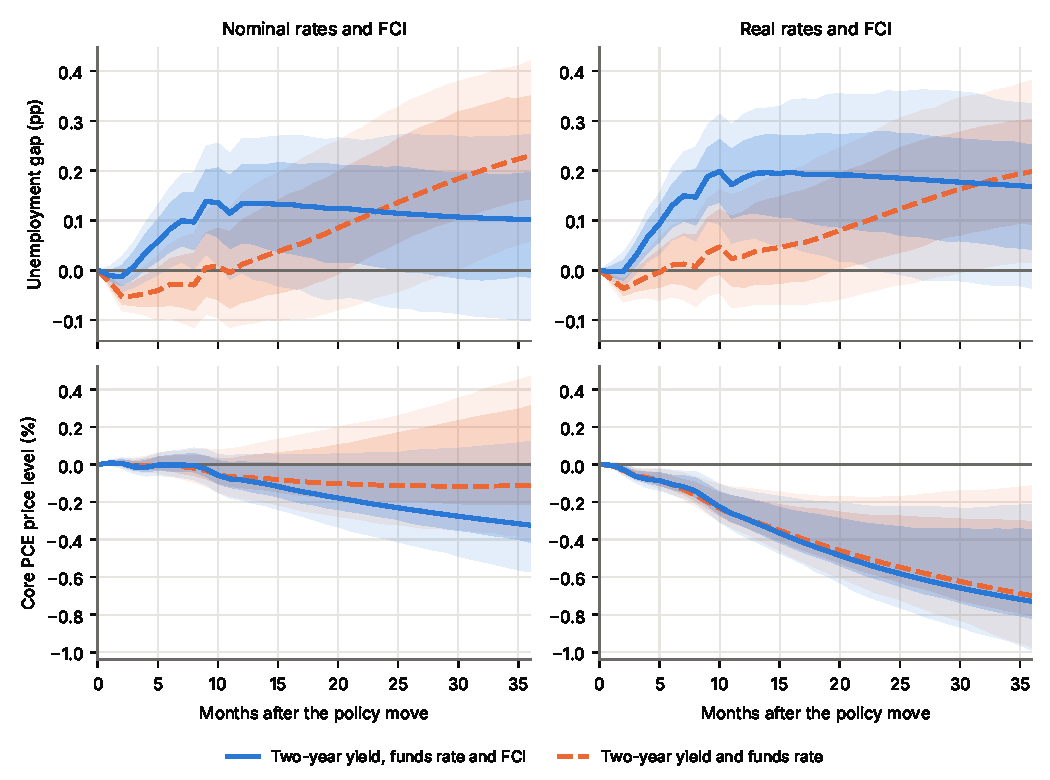
\includegraphics[width=\textwidth]{../baseline_real/report/fig_steps73.pdf}
\caption{Responses to a Policy Move, without and with the FCI, Monthly Equations from 1973}
\label{fig:steps73}
\begin{flushleft}\footnotesize\textit{Notes:} Policy move that raises the two-year yield 1 percentage point in the window; monthly equations from 1973; 12 lags. Orange dashed: the two-year yield and the funds rate alone. Blue: the same rates and the FCI of the same version. Bands: 68 and 90 percent intervals.\end{flushleft}
\end{figure}

\begin{figure}[tp]
\centering
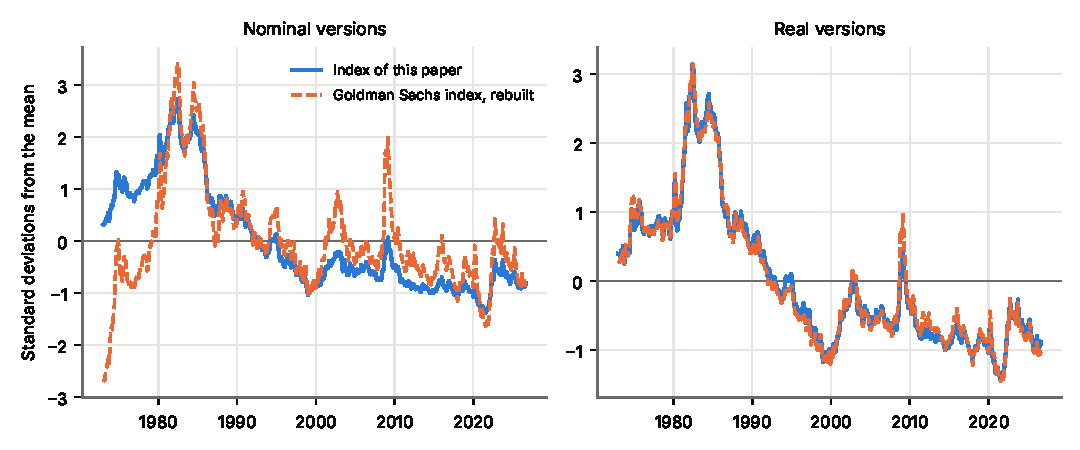
\includegraphics[width=\textwidth]{../baseline_real/report/fig_gs.pdf}
\caption{The Index and the Goldman Sachs Index, Nominal and Real Versions}
\label{fig:gs}
\begin{flushleft}\footnotesize\textit{Notes:} Monthly, January 1973 to September 2026, each series in units of its standard deviation from its mean. The Goldman Sachs index is rebuilt from public data with its published weights (companion paper), in the same version as the index of this paper. Left: nominal versions. Right: real versions, with the 10-year yield less 10-year expected inflation.\end{flushleft}
\end{figure}

\begin{figure}[tp]
\centering
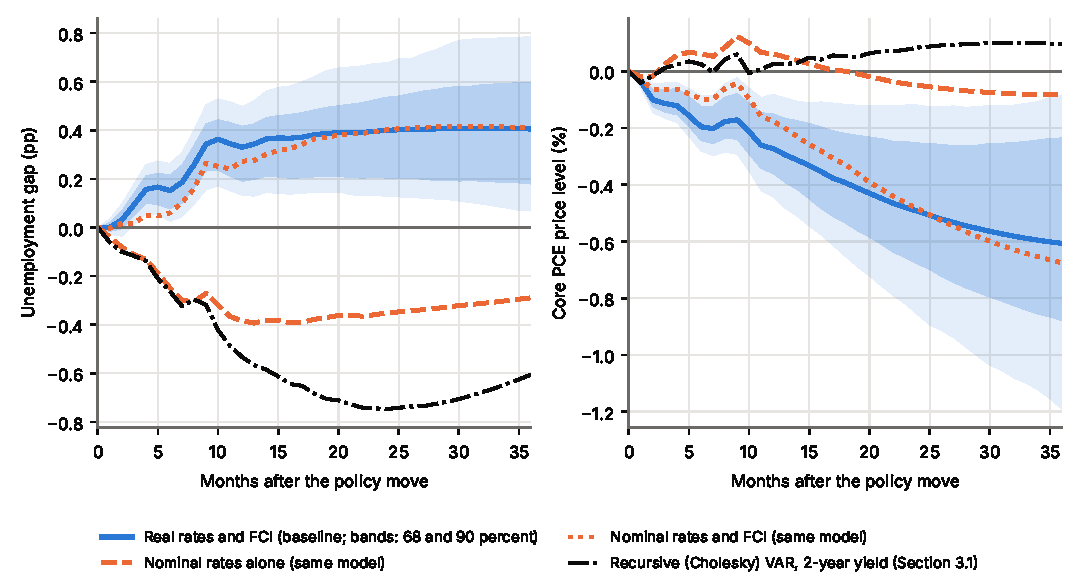
\includegraphics[width=\textwidth]{../baseline_real/report/fig_size.pdf}
\caption{Responses to a Policy Move: Baseline, Nominal Rates Alone and with the FCI, and Cholesky VAR}
\label{fig:size}
\begin{flushleft}\footnotesize\textit{Notes:} Policy move that raises the two-year yield 1 percentage point. Baseline: real two-year yield, funds rate and FCI; 12 lags; shaded bands 68 and 90 percent. The nominal rates alone and with the FCI are in the same model; the Cholesky VAR is that of Section~\ref{sec:standard}.\end{flushleft}
\end{figure}

\begin{table}[tp]\centering\footnotesize\setlength{\tabcolsep}{2.2pt}
\caption{Baselines: Monthly Equations from 1996 and from 1973, March-December 2020 Dropped (12 Lags)}\label{tab:mainB}
\resizebox{\ifdim\width>\textwidth\textwidth\else\width\fi}{!}{%
\begin{tabular}{llcrrrrrrr}\toprule
 & & & & \multicolumn{3}{c}{Unemployment gap (pp)} & \multicolumn{3}{c}{Price level (\%)}\\ \cmidrule(lr){5-7}\cmidrule(lr){8-10}
Case & FCI & Lags & Obs & 12 m & 24 m & 36 m & 12 m & 24 m & 36 m\\ \midrule
Baseline, 1996: Nominal & none & 12 & 359 & $-$0.38$^{**}$ & $-$0.35$^{**}$ & $-$0.29$^{**}$ & 0.06 & $-$0.05 & $-$0.08\\
 & & & & {\scriptsize [$-$0.63, $-$0.17]} & {\scriptsize [$-$0.71, $-$0.10]} & {\scriptsize [$-$0.81, $-$0.06]} & {\scriptsize [$-$0.13, 0.25]} & {\scriptsize [$-$0.46, 0.32]} & {\scriptsize [$-$0.71, 0.38]}\\
 & nominal & 12 & 359 & 0.27$^{**}$ & 0.40$^{**}$ & 0.41$^{**}$ & $-$0.18 & $-$0.49$^{**}$ & $-$0.68$^{**}$\\
 & & & & {\scriptsize [0.08, 0.53]} & {\scriptsize [0.16, 0.82]} & {\scriptsize [0.20, 1.19]} & {\scriptsize [$-$0.39, 0.04]} & {\scriptsize [$-$0.94, $-$0.13]} & {\scriptsize [$-$1.63, $-$0.24]}\\
\addlinespace
Baseline, 1996: Real & none & 12 & 359 & $-$0.24$^{*}$ & $-$0.33$^{**}$ & $-$0.25$^{**}$ & $-$0.07 & $-$0.06 & $-$0.05\\
 & & & & {\scriptsize [$-$0.42, $-$0.04]} & {\scriptsize [$-$0.63, $-$0.11]} & {\scriptsize [$-$0.73, $-$0.05]} & {\scriptsize [$-$0.25, 0.07]} & {\scriptsize [$-$0.35, 0.21]} & {\scriptsize [$-$0.41, 0.34]}\\
 & real & 12 & 359 & 0.33$^{**}$ & 0.40$^{**}$ & 0.41$^{**}$ & $-$0.27$^{**}$ & $-$0.49$^{**}$ & $-$0.61$^{**}$\\
 & & & & {\scriptsize [0.16, 0.56]} & {\scriptsize [0.18, 0.78]} & {\scriptsize [0.15, 0.96]} & {\scriptsize [$-$0.48, $-$0.13]} & {\scriptsize [$-$0.93, $-$0.17]} & {\scriptsize [$-$1.39, $-$0.17]}\\
\addlinespace
Baseline, 1973: Nominal & none & 12 & 623 & 0.01 & 0.13 & 0.23 & $-$0.07 & $-$0.11 & $-$0.11\\
 & & & & {\scriptsize [$-$0.11, 0.15]} & {\scriptsize [$-$0.09, 0.28]} & {\scriptsize [$-$0.02, 0.39]} & {\scriptsize [$-$0.23, 0.04]} & {\scriptsize [$-$0.44, 0.08]} & {\scriptsize [$-$0.62, 0.16]}\\
 & nominal & 12 & 623 & 0.13$^{*}$ & 0.12 & 0.10 & $-$0.08 & $-$0.22$^{**}$ & $-$0.32$^{**}$\\
 & & & & {\scriptsize [0.01, 0.28]} & {\scriptsize [$-$0.05, 0.28]} & {\scriptsize [$-$0.08, 0.30]} & {\scriptsize [$-$0.24, 0.00]} & {\scriptsize [$-$0.58, $-$0.06]} & {\scriptsize [$-$0.97, $-$0.12]}\\
\addlinespace
Baseline, 1973: Real & none & 12 & 623 & 0.03 & 0.11 & 0.20$^{*}$ & $-$0.28$^{**}$ & $-$0.53$^{**}$ & $-$0.70$^{**}$\\
 & & & & {\scriptsize [$-$0.10, 0.14]} & {\scriptsize [$-$0.06, 0.26]} & {\scriptsize [0.01, 0.37]} & {\scriptsize [$-$0.43, $-$0.18]} & {\scriptsize [$-$0.87, $-$0.33]} & {\scriptsize [$-$1.34, $-$0.40]}\\
 & real & 12 & 623 & 0.19$^{**}$ & 0.19$^{**}$ & 0.17$^{**}$ & $-$0.28$^{**}$ & $-$0.56$^{**}$ & $-$0.73$^{**}$\\
 & & & & {\scriptsize [0.07, 0.32]} & {\scriptsize [0.05, 0.40]} & {\scriptsize [0.04, 0.44]} & {\scriptsize [$-$0.42, $-$0.18]} & {\scriptsize [$-$0.94, $-$0.38]} & {\scriptsize [$-$1.43, $-$0.47]}\\
\bottomrule\end{tabular}}
\begin{flushleft}\footnotesize\textit{Notes:} Nominal and real 2-year yield and funds rate; the FCI is the index in the matching form in each case. March-December 2020 dropped from the monthly and daily equations (values still enter as lags). From 1973: monthly series in place of daily data before 1990. Per +1 pp on the 2-year yield in the window unless stated. $^{**}$ and $^{*}$: significant at the 5 and 10 percent levels (the 95\% and 90\% bootstrap intervals exclude zero); 90\% intervals in brackets. Obs = monthly observations in the equations.\end{flushleft}
\end{table}

\FloatBarrier
\begin{table}[tp]\centering\small
\caption{Implied Trade-Off: Phillips Multiplier $\kappa_H$ (12 Lags), All Cases}\label{tab:tradefull}
\resizebox{\ifdim\width>\textwidth\textwidth\else\width\fi}{!}{%
\begin{tabular}{llrrrr}\toprule & & \multicolumn{2}{c}{Multiplier $\kappa_H$} & \multicolumn{2}{c}{Cost (sacrifice ratio)}\\ \cmidrule(lr){3-4}\cmidrule(lr){5-6} Case & FCI & $H=24$ & $H=36$ & $H=24$ & $H=36$\\ \midrule
\multicolumn{6}{l}{\textit{Baseline, 1996}}\\
Nominal & none & 0.08 [$-$0.36, 1.38] & 0.09 [$-$0.29, 1.48] & not defined & not defined\\
 & nominal & $-$1.02 [$-$2.38, $-$0.29]$^{\dagger}$ & $-$0.76 [$-$1.64, $-$0.29] & 0.98 [0.42, 3.49] & 1.32 [0.61, 3.41]$^{\dagger}$\\
Real & none & 0.16 [$-$0.45, 2.27] & 0.07 [$-$0.42, 1.44] & not defined & not defined\\
 & real & $-$0.85 [$-$1.45, $-$0.33] & $-$0.61 [$-$1.08, $-$0.18] & 1.18 [0.69, 3.03] & 1.63 [0.93, 5.41]\\
\addlinespace
\multicolumn{6}{l}{\textit{Baseline, 1973}}\\
Nominal & none & $-$2.32 (undefined; 68\%: undefined) & $-$0.48 (undefined; 68\%: undefined) & 0.43 (unbounded) & 2.08 (unbounded)\\
 & nominal & $-$1.11 (undefined; 68\%: [$-$3.57, $-$0.64]) & $-$1.05 (undefined; 68\%: [$-$4.06, $-$0.72]) & 0.90 [$-$0.06, 3.09] & 0.95 [$-$0.10, 2.65]\\
Real & none & $-$6.94 (undefined; 68\%: undefined) & $-$2.90 (undefined; 68\%: undefined) & 0.14 [$-$0.34, 0.47] & 0.34 [$-$0.23, 0.82]\\
 & real & $-$1.85 [$-$5.37, $-$1.16] & $-$1.52 [$-$4.92, $-$0.92] & 0.54 [0.19, 0.86] & 0.66 [0.20, 1.09]\\
\addlinespace
\multicolumn{6}{l}{\textit{Robustness tests and the final section, real with the FCI}}\\
2020 left in, 1996 & real & $-$1.21 (undefined; 68\%: [$-$2.80, $-$0.73]) & $-$0.93 (undefined; 68\%: [$-$1.95, $-$0.58]) & 0.83 [$-$0.08, 1.90] & 1.07 [$-$0.02, 2.71]\\
2020 left in, 1973 & real & $-$13.29 (undefined; 68\%: undefined) & $-$5.84 (undefined; 68\%: undefined) & 0.08 [$-$0.74, 0.75] & 0.17 [$-$0.78, 1.35]\\
IP added, 1996 & real & $-$0.90 [$-$1.61, $-$0.41] & $-$0.60 [$-$1.08, $-$0.20] & 1.12 [0.62, 2.44] & 1.67 [0.92, 5.12]\\
IP added, 1973 & real & $-$0.80 [$-$1.48, $-$0.52] & $-$0.50 [$-$0.98, $-$0.23] & 1.25 [0.68, 1.92] & 1.98 [1.02, 4.41]\\
Bauer-Swanson surprise, 1996 & real & $-$0.80 [$-$1.34, $-$0.33] & $-$0.59 [$-$1.00, $-$0.19] & 1.24 [0.74, 3.04] & 1.71 [1.00, 5.29]\\
Bauer-Swanson surprise, 1973 & real & $-$1.57 [$-$3.29, $-$1.01] & $-$1.30 [$-$3.17, $-$0.76] & 0.64 [0.30, 0.99] & 0.77 [0.32, 1.31]\\
Without the funds rate, 1996 & real & $-$1.16 [$-$7.10, $-$0.30] & $-$0.90 [$-$228.66, $-$0.11] & 0.86 [0.14, 3.38] & 1.11 [0.00, 9.33]$^{\dagger}$\\
Without the funds rate, 1973 & real & $-$1.56 [$-$3.24, $-$0.95] & $-$1.89 [$-$5.30, $-$1.00] & 0.64 [0.31, 1.05] & 0.53 [0.19, 1.00]\\
Monthly equations from 1985 & real & $-$0.64 [$-$3.79, 10.49]$^{\dagger}$ & $-$0.26 (undefined; 68\%: [$-$1.06, 0.24]) & 1.57 (unbounded) & 3.85 (unbounded)\\
Cubic spline trend, 1996 & real & $-$0.44 [$-$1.05, 0.65] & $-$0.22 [$-$0.69, 0.83] & 2.25 (unbounded) & 4.47 (unbounded)\\
Cubic spline trend, 1973 & real & $-$1.06 [$-$2.26, $-$0.61] & $-$0.74 [$-$1.59, $-$0.42] & 0.94 [0.44, 1.63] & 1.34 [0.63, 2.38]\\
Ends 2019, 1996 & real & 0.42 (undefined; 68\%: [0.13, 1.32]) & 0.31 (undefined; 68\%: [0.06, 11.18]) & not defined & not defined\\
Ends 2019, 1973 & real & $-$1.32 [$-$12.76, $-$0.64] & $-$1.30 [$-$73.92, $-$0.51] & 0.76 [0.08, 1.57] & 0.77 [0.01, 1.95]\\
r*-gap (LW), 1996 & r*-gap & $-$1.06 [$-$1.73, $-$0.69] & $-$0.83 [$-$1.59, $-$0.49] & 0.94 [0.58, 1.44] & 1.21 [0.63, 2.03]\\
r*-gap (LW), 1973 & r*-gap & $-$1.32 [$-$3.02, $-$0.92] & $-$1.03 [$-$2.86, $-$0.71] & 0.76 [0.33, 1.09] & 0.97 [0.35, 1.41]\\
\addlinespace
Real minus nominal, with FCI & & [$-$0.97, 1.96] & [$-$0.78, 1.67] & & \\
\bottomrule\end{tabular}}
\begin{flushleft}\footnotesize\textit{Notes:} $\kappa_H$ = core PCE price level at month $H$ (percent) per percentage-point year of cumulative unemployment-gap response (Barnichon and Mesters 2021); the sacrifice ratio is $-1/\kappa_H$. Point estimate and 90\% confidence set (Anderson--Rubin type) in brackets, computed exactly (a wide grid refined by bisection), so a finite end is never an artifact of the grid. An infinite end means that the 90\% interval of the cumulative unemployment response includes zero: the data then cannot rule out arbitrarily steep trade-offs on that side; ``unbounded'': both sides. $^{\dagger}$: the set has a gap wider than 2 percent of its width; shown is its hull. Ends 2019: all equations end in December 2019 (2020 not dropped). Cost: percentage-point years of cumulative unemployment per 1 percent lower price level, with the 90\% set obtained by inverting the test for the cost itself (bounded whenever the price response is well estimated; ``not defined'' where the price level does not fall). Last row: paired difference over common announcement draws.\end{flushleft}
\end{table}

\FloatBarrier
\begin{table}[tp]\centering\footnotesize\setlength{\tabcolsep}{2.2pt}
\caption{Robustness Tests (12 Lags)}\label{tab:mainR}
\resizebox{\ifdim\width>\textwidth\textwidth\else\width\fi}{!}{%
\begin{tabular}{llcrrrrrrr}\toprule
 & & & & \multicolumn{3}{c}{Unemployment gap (pp)} & \multicolumn{3}{c}{Price level (\%)}\\ \cmidrule(lr){5-7}\cmidrule(lr){8-10}
Case & FCI & Lags & Obs & 12 m & 24 m & 36 m & 12 m & 24 m & 36 m\\ \midrule
2020 left in, 1996: Nominal & none & 12 & 369 & $-$0.62$^{**}$ & $-$0.37 & $-$0.37 & 0.19 & $-$0.05 & $-$0.19\\
 & & & & {\scriptsize [$-$1.17, $-$0.18]} & {\scriptsize [$-$0.84, 0.03]} & {\scriptsize [$-$0.78, 0.05]} & {\scriptsize [$-$0.03, 0.48]} & {\scriptsize [$-$0.47, 0.41]} & {\scriptsize [$-$0.74, 0.40]}\\
 & nominal & 12 & 369 & 0.35 & 0.25 & 0.15 & $-$0.18 & $-$0.59$^{**}$ & $-$0.82$^{**}$\\
 & & & & {\scriptsize [$-$0.12, 0.76]} & {\scriptsize [$-$0.08, 0.81]} & {\scriptsize [$-$0.16, 0.85]} & {\scriptsize [$-$0.42, 0.03]} & {\scriptsize [$-$1.08, $-$0.23]} & {\scriptsize [$-$1.63, $-$0.34]}\\
\addlinespace
2020 left in, 1996: Real & none & 12 & 369 & $-$0.60$^{**}$ & $-$0.37$^{**}$ & $-$0.22 & 0.00 & $-$0.07 & $-$0.17\\
 & & & & {\scriptsize [$-$1.06, $-$0.26]} & {\scriptsize [$-$0.80, $-$0.12]} & {\scriptsize [$-$0.69, 0.06]} & {\scriptsize [$-$0.20, 0.20]} & {\scriptsize [$-$0.41, 0.29]} & {\scriptsize [$-$0.68, 0.36]}\\
 & real & 12 & 369 & 0.24 & 0.30 & 0.26 & $-$0.30$^{**}$ & $-$0.56$^{**}$ & $-$0.70$^{**}$\\
 & & & & {\scriptsize [$-$0.20, 0.66]} & {\scriptsize [$-$0.04, 0.75]} & {\scriptsize [$-$0.08, 0.83]} & {\scriptsize [$-$0.54, $-$0.12]} & {\scriptsize [$-$1.12, $-$0.25]} & {\scriptsize [$-$1.60, $-$0.25]}\\
\addlinespace
2020 left in, 1973: Nominal & none & 12 & 633 & $-$0.37$^{**}$ & $-$0.17$^{**}$ & 0.00 & 0.04 & 0.11 & 0.20\\
 & & & & {\scriptsize [$-$0.62, $-$0.25]} & {\scriptsize [$-$0.64, $-$0.07]} & {\scriptsize [$-$0.37, 0.13]} & {\scriptsize [$-$0.16, 0.15]} & {\scriptsize [$-$0.34, 0.29]} & {\scriptsize [$-$0.71, 0.44]}\\
 & nominal & 12 & 633 & $-$0.13 & $-$0.13 & $-$0.09 & 0.02 & 0.05 & 0.08\\
 & & & & {\scriptsize [$-$0.35, 0.07]} & {\scriptsize [$-$0.39, 0.08]} & {\scriptsize [$-$0.39, 0.13]} & {\scriptsize [$-$0.14, 0.13]} & {\scriptsize [$-$0.31, 0.24]} & {\scriptsize [$-$0.48, 0.36]}\\
\addlinespace
2020 left in, 1973: Real & none & 12 & 633 & $-$0.22$^{**}$ & $-$0.07 & 0.07 & $-$0.20$^{**}$ & $-$0.36$^{**}$ & $-$0.47$^{**}$\\
 & & & & {\scriptsize [$-$0.40, $-$0.10]} & {\scriptsize [$-$0.26, 0.07]} & {\scriptsize [$-$0.14, 0.22]} & {\scriptsize [$-$0.33, $-$0.10]} & {\scriptsize [$-$0.70, $-$0.17]} & {\scriptsize [$-$1.19, $-$0.18]}\\
 & real & 12 & 633 & 0.02 & 0.03 & 0.05 & $-$0.21$^{**}$ & $-$0.37$^{**}$ & $-$0.44$^{**}$\\
 & & & & {\scriptsize [$-$0.16, 0.22]} & {\scriptsize [$-$0.15, 0.25]} & {\scriptsize [$-$0.10, 0.38]} & {\scriptsize [$-$0.36, $-$0.10]} & {\scriptsize [$-$0.70, $-$0.19]} & {\scriptsize [$-$1.04, $-$0.15]}\\
\addlinespace
IP added, 1996: Nominal & none & 12 & 359 & $-$0.29$^{**}$ & $-$0.02 & 0.15 & 0.13 & 0.13 & 0.24\\
 & & & & {\scriptsize [$-$0.49, $-$0.09]} & {\scriptsize [$-$0.26, 0.32]} & {\scriptsize [$-$0.13, 0.63]} & {\scriptsize [$-$0.03, 0.32]} & {\scriptsize [$-$0.17, 0.45]} & {\scriptsize [$-$0.21, 0.81]}\\
 & nominal & 12 & 359 & 0.23$^{**}$ & 0.50$^{**}$ & 0.55$^{**}$ & $-$0.25$^{*}$ & $-$0.55$^{**}$ & $-$0.72$^{*}$\\
 & & & & {\scriptsize [0.03, 0.51]} & {\scriptsize [0.19, 0.94]} & {\scriptsize [0.22, 1.25]} & {\scriptsize [$-$0.45, $-$0.04]} & {\scriptsize [$-$0.92, $-$0.09]} & {\scriptsize [$-$1.38, $-$0.07]}\\
\addlinespace
IP added, 1996: Real & none & 12 & 359 & $-$0.18 & $-$0.07 & 0.18 & 0.00 & 0.05 & 0.09\\
 & & & & {\scriptsize [$-$0.34, 0.04]} & {\scriptsize [$-$0.35, 0.19]} & {\scriptsize [$-$0.10, 0.53]} & {\scriptsize [$-$0.16, 0.14]} & {\scriptsize [$-$0.25, 0.30]} & {\scriptsize [$-$0.32, 0.51]}\\
 & real & 12 & 359 & 0.31$^{**}$ & 0.52$^{**}$ & 0.59$^{**}$ & $-$0.32$^{**}$ & $-$0.55$^{**}$ & $-$0.70$^{**}$\\
 & & & & {\scriptsize [0.16, 0.60]} & {\scriptsize [0.30, 0.95]} & {\scriptsize [0.29, 1.20]} & {\scriptsize [$-$0.53, $-$0.16]} & {\scriptsize [$-$0.96, $-$0.21]} & {\scriptsize [$-$1.39, $-$0.22]}\\
\addlinespace
IP added, 1973: Nominal & none & 12 & 623 & 0.10 & 0.29$^{**}$ & 0.42$^{**}$ & $-$0.07 & $-$0.13 & $-$0.14\\
 & & & & {\scriptsize [$-$0.05, 0.24]} & {\scriptsize [0.13, 0.50]} & {\scriptsize [0.25, 0.67]} & {\scriptsize [$-$0.21, 0.02]} & {\scriptsize [$-$0.40, 0.02]} & {\scriptsize [$-$0.52, 0.06]}\\
 & nominal & 12 & 623 & 0.21$^{**}$ & 0.26$^{**}$ & 0.24$^{**}$ & $-$0.07 & $-$0.15$^{*}$ & $-$0.18$^{*}$\\
 & & & & {\scriptsize [0.09, 0.35]} & {\scriptsize [0.12, 0.45]} & {\scriptsize [0.11, 0.48]} & {\scriptsize [$-$0.22, 0.02]} & {\scriptsize [$-$0.42, $-$0.02]} & {\scriptsize [$-$0.50, 0.00]}\\
\addlinespace
IP added, 1973: Real & none & 12 & 623 & 0.10 & 0.28$^{**}$ & 0.37$^{**}$ & $-$0.22$^{**}$ & $-$0.32$^{**}$ & $-$0.35$^{**}$\\
 & & & & {\scriptsize [$-$0.02, 0.21]} & {\scriptsize [0.12, 0.44]} & {\scriptsize [0.22, 0.62]} & {\scriptsize [$-$0.36, $-$0.14]} & {\scriptsize [$-$0.57, $-$0.18]} & {\scriptsize [$-$0.75, $-$0.15]}\\
 & real & 12 & 623 & 0.25$^{**}$ & 0.30$^{**}$ & 0.24$^{**}$ & $-$0.23$^{**}$ & $-$0.35$^{**}$ & $-$0.36$^{**}$\\
 & & & & {\scriptsize [0.13, 0.41]} & {\scriptsize [0.15, 0.52]} & {\scriptsize [0.09, 0.52]} & {\scriptsize [$-$0.38, $-$0.15]} & {\scriptsize [$-$0.63, $-$0.20]} & {\scriptsize [$-$0.81, $-$0.15]}\\
\addlinespace
Bauer-Swanson surprise, 1996: Nominal & none & 12 & 359 & $-$0.38$^{**}$ & $-$0.35$^{**}$ & $-$0.29$^{**}$ & 0.06 & $-$0.05 & $-$0.08\\
 & & & & {\scriptsize [$-$0.63, $-$0.17]} & {\scriptsize [$-$0.71, $-$0.10]} & {\scriptsize [$-$0.81, $-$0.06]} & {\scriptsize [$-$0.13, 0.25]} & {\scriptsize [$-$0.47, 0.32]} & {\scriptsize [$-$0.71, 0.38]}\\
 & nominal & 12 & 359 & 0.32$^{**}$ & 0.45$^{**}$ & 0.45$^{**}$ & $-$0.19 & $-$0.52$^{**}$ & $-$0.72$^{**}$\\
 & & & & {\scriptsize [0.13, 0.59]} & {\scriptsize [0.23, 1.01]} & {\scriptsize [0.22, 1.28]} & {\scriptsize [$-$0.41, 0.03]} & {\scriptsize [$-$1.01, $-$0.14]} & {\scriptsize [$-$1.80, $-$0.27]}\\
\addlinespace
Bauer-Swanson surprise, 1996: Real & none & 12 & 359 & $-$0.24$^{*}$ & $-$0.33$^{**}$ & $-$0.25$^{**}$ & $-$0.07 & $-$0.06 & $-$0.05\\
 & & & & {\scriptsize [$-$0.42, $-$0.04]} & {\scriptsize [$-$0.63, $-$0.11]} & {\scriptsize [$-$0.73, $-$0.05]} & {\scriptsize [$-$0.25, 0.07]} & {\scriptsize [$-$0.35, 0.21]} & {\scriptsize [$-$0.41, 0.34]}\\
 & real & 12 & 359 & 0.37$^{**}$ & 0.45$^{**}$ & 0.44$^{**}$ & $-$0.29$^{**}$ & $-$0.52$^{**}$ & $-$0.64$^{**}$\\
 & & & & {\scriptsize [0.20, 0.62]} & {\scriptsize [0.21, 0.90]} & {\scriptsize [0.18, 1.07]} & {\scriptsize [$-$0.52, $-$0.14]} & {\scriptsize [$-$1.01, $-$0.20]} & {\scriptsize [$-$1.49, $-$0.18]}\\
\addlinespace
Bauer-Swanson surprise, 1973: Nominal & none & 12 & 623 & 0.01 & 0.13 & 0.23 & $-$0.07 & $-$0.11 & $-$0.11\\
 & & & & {\scriptsize [$-$0.11, 0.15]} & {\scriptsize [$-$0.09, 0.28]} & {\scriptsize [$-$0.02, 0.39]} & {\scriptsize [$-$0.23, 0.04]} & {\scriptsize [$-$0.44, 0.08]} & {\scriptsize [$-$0.62, 0.16]}\\
 & nominal & 12 & 623 & 0.17$^{**}$ & 0.14 & 0.11 & $-$0.08 & $-$0.21$^{**}$ & $-$0.31$^{**}$\\
 & & & & {\scriptsize [0.04, 0.31]} & {\scriptsize [$-$0.01, 0.33]} & {\scriptsize [$-$0.07, 0.32]} & {\scriptsize [$-$0.24, 0.01]} & {\scriptsize [$-$0.60, $-$0.06]} & {\scriptsize [$-$0.96, $-$0.09]}\\
\addlinespace
Bauer-Swanson surprise, 1973: Real & none & 12 & 623 & 0.03 & 0.11 & 0.20$^{*}$ & $-$0.28$^{**}$ & $-$0.53$^{**}$ & $-$0.70$^{**}$\\
 & & & & {\scriptsize [$-$0.10, 0.14]} & {\scriptsize [$-$0.06, 0.26]} & {\scriptsize [0.01, 0.37]} & {\scriptsize [$-$0.43, $-$0.18]} & {\scriptsize [$-$0.87, $-$0.33]} & {\scriptsize [$-$1.34, $-$0.40]}\\
 & real & 12 & 623 & 0.22$^{**}$ & 0.21$^{**}$ & 0.18$^{**}$ & $-$0.28$^{**}$ & $-$0.56$^{**}$ & $-$0.72$^{**}$\\
 & & & & {\scriptsize [0.11, 0.37]} & {\scriptsize [0.08, 0.43]} & {\scriptsize [0.04, 0.47]} & {\scriptsize [$-$0.43, $-$0.18]} & {\scriptsize [$-$0.94, $-$0.38]} & {\scriptsize [$-$1.42, $-$0.47]}\\
\addlinespace
Without the funds rate, 1996: Nominal & none & 12 & 359 & $-$0.37$^{**}$ & $-$0.45$^{**}$ & $-$0.37$^{**}$ & 0.01 & 0.06 & 0.06\\
 & & & & {\scriptsize [$-$0.56, $-$0.19]} & {\scriptsize [$-$0.85, $-$0.26]} & {\scriptsize [$-$0.84, $-$0.16]} & {\scriptsize [$-$0.15, 0.17]} & {\scriptsize [$-$0.22, 0.37]} & {\scriptsize [$-$0.33, 0.56]}\\
 & nominal & 12 & 359 & 0.13 & 0.16 & 0.16 & $-$0.14 & $-$0.29 & $-$0.42\\
 & & & & {\scriptsize [$-$0.07, 0.34]} & {\scriptsize [$-$0.19, 0.41]} & {\scriptsize [$-$0.26, 0.44]} & {\scriptsize [$-$0.33, 0.07]} & {\scriptsize [$-$0.66, 0.14]} & {\scriptsize [$-$0.98, 0.17]}\\
\addlinespace
Without the funds rate, 1996: Real & none & 12 & 359 & $-$0.28$^{**}$ & $-$0.35$^{**}$ & $-$0.30$^{**}$ & $-$0.08 & $-$0.06 & $-$0.06\\
 & & & & {\scriptsize [$-$0.44, $-$0.11]} & {\scriptsize [$-$0.64, $-$0.15]} & {\scriptsize [$-$0.67, $-$0.10]} & {\scriptsize [$-$0.25, 0.03]} & {\scriptsize [$-$0.34, 0.15]} & {\scriptsize [$-$0.41, 0.25]}\\
 & real & 12 & 359 & 0.17$^{*}$ & 0.23 & 0.22 & $-$0.22$^{**}$ & $-$0.38$^{**}$ & $-$0.50$^{*}$\\
 & & & & {\scriptsize [0.02, 0.35]} & {\scriptsize [$-$0.01, 0.48]} & {\scriptsize [$-$0.05, 0.55]} & {\scriptsize [$-$0.40, $-$0.07]} & {\scriptsize [$-$0.76, $-$0.08]} & {\scriptsize [$-$1.04, $-$0.06]}\\
\addlinespace
Without the funds rate, 1973: Nominal & none & 12 & 623 & 0.11$^{*}$ & 0.17$^{**}$ & 0.13$^{**}$ & $-$0.01 & $-$0.08 & $-$0.15\\
 & & & & {\scriptsize [0.00, 0.25]} & {\scriptsize [0.08, 0.37]} & {\scriptsize [0.05, 0.30]} & {\scriptsize [$-$0.15, 0.09]} & {\scriptsize [$-$0.39, 0.11]} & {\scriptsize [$-$0.65, 0.08]}\\
 & nominal & 12 & 623 & 0.29$^{**}$ & 0.19$^{**}$ & 0.06 & $-$0.01 & $-$0.17$^{*}$ & $-$0.33$^{**}$\\
 & & & & {\scriptsize [0.17, 0.45]} & {\scriptsize [0.09, 0.46]} & {\scriptsize [$-$0.06, 0.27]} & {\scriptsize [$-$0.17, 0.08]} & {\scriptsize [$-$0.43, $-$0.01]} & {\scriptsize [$-$0.79, $-$0.16]}\\
\addlinespace
Without the funds rate, 1973: Real & none & 12 & 623 & 0.09 & 0.08 & 0.02 & $-$0.23$^{**}$ & $-$0.49$^{**}$ & $-$0.72$^{**}$\\
 & & & & {\scriptsize [$-$0.01, 0.22]} & {\scriptsize [$-$0.03, 0.23]} & {\scriptsize [$-$0.09, 0.19]} & {\scriptsize [$-$0.35, $-$0.14]} & {\scriptsize [$-$0.78, $-$0.33]} & {\scriptsize [$-$1.32, $-$0.49]}\\
 & real & 12 & 623 & 0.25$^{**}$ & 0.13$^{*}$ & 0.02 & $-$0.24$^{**}$ & $-$0.55$^{**}$ & $-$0.79$^{**}$\\
 & & & & {\scriptsize [0.14, 0.40]} & {\scriptsize [0.01, 0.33]} & {\scriptsize [$-$0.09, 0.25]} & {\scriptsize [$-$0.38, $-$0.15]} & {\scriptsize [$-$0.85, $-$0.40]} & {\scriptsize [$-$1.33, $-$0.59]}\\
\addlinespace
Monthly equations from 1985: Nominal & none & 12 & 491 & $-$0.23$^{**}$ & $-$0.29$^{**}$ & $-$0.23$^{**}$ & 0.06 & 0.15 & 0.28\\
 & & & & {\scriptsize [$-$0.37, $-$0.10]} & {\scriptsize [$-$0.55, $-$0.13]} & {\scriptsize [$-$0.49, $-$0.06]} & {\scriptsize [$-$0.06, 0.19]} & {\scriptsize [$-$0.06, 0.41]} & {\scriptsize [$-$0.03, 0.64]}\\
 & nominal & 12 & 491 & 0.04 & 0.01 & 0.00 & 0.02 & 0.03 & 0.10\\
 & & & & {\scriptsize [$-$0.10, 0.18]} & {\scriptsize [$-$0.16, 0.18]} & {\scriptsize [$-$0.20, 0.21]} & {\scriptsize [$-$0.11, 0.15]} & {\scriptsize [$-$0.22, 0.22]} & {\scriptsize [$-$0.20, 0.33]}\\
\addlinespace
Monthly equations from 1985: Real & none & 12 & 491 & $-$0.15$^{*}$ & $-$0.21$^{**}$ & $-$0.14 & $-$0.02 & 0.02 & 0.11\\
 & & & & {\scriptsize [$-$0.27, 0.00]} & {\scriptsize [$-$0.41, $-$0.05]} & {\scriptsize [$-$0.43, 0.00]} & {\scriptsize [$-$0.15, 0.09]} & {\scriptsize [$-$0.22, 0.27]} & {\scriptsize [$-$0.23, 0.45]}\\
 & real & 12 & 491 & 0.12$^{*}$ & 0.11 & 0.10 & $-$0.07 & $-$0.11 & $-$0.07\\
 & & & & {\scriptsize [0.00, 0.32]} & {\scriptsize [$-$0.03, 0.40]} & {\scriptsize [$-$0.10, 0.32]} & {\scriptsize [$-$0.24, 0.04]} & {\scriptsize [$-$0.42, 0.08]} & {\scriptsize [$-$0.43, 0.18]}\\
\bottomrule\end{tabular}}
\begin{flushleft}\footnotesize\textit{Notes:} 2020 left in: no month dummies. IP added: industrial production as a further monthly variable. Bauer-Swanson: orthogonalized surprise, announcements through 2019. Without the funds rate: the 2-year yield is the only rate in the daily block. From 1985: monthly equations from January 1985. Lag length: every case at 6 lags in the appendix tables. Per +1 pp on the 2-year yield in the window unless stated. $^{**}$ and $^{*}$: significant at the 5 and 10 percent levels (the 95\% and 90\% bootstrap intervals exclude zero); 90\% intervals in brackets. Obs = monthly observations in the equations.\end{flushleft}
\end{table}

\FloatBarrier
\begin{table}[tp]\centering\footnotesize\setlength{\tabcolsep}{2.2pt}
\caption{Slow-Moving Rates: The r*-gap Step and a Spline Trend (12 Lags)}\label{tab:mainF}
\resizebox{\ifdim\width>\textwidth\textwidth\else\width\fi}{!}{%
\begin{tabular}{llcrrrrrrr}\toprule
 & & & & \multicolumn{3}{c}{Unemployment gap (pp)} & \multicolumn{3}{c}{Price level (\%)}\\ \cmidrule(lr){5-7}\cmidrule(lr){8-10}
Case & FCI & Lags & Obs & 12 m & 24 m & 36 m & 12 m & 24 m & 36 m\\ \midrule
r*-gap (LW), 1996 & none & 12 & 359 & 0.02 & $-$0.11 & $-$0.07 & $-$0.22$^{*}$ & $-$0.38$^{*}$ & $-$0.47\\
 & & & & {\scriptsize [$-$0.18, 0.22]} & {\scriptsize [$-$0.42, 0.24]} & {\scriptsize [$-$0.41, 0.36]} & {\scriptsize [$-$0.37, $-$0.04]} & {\scriptsize [$-$0.70, 0.00]} & {\scriptsize [$-$0.95, 0.07]}\\
 & r*-gap & 12 & 359 & 0.43$^{**}$ & 0.49$^{**}$ & 0.49$^{*}$ & $-$0.42$^{**}$ & $-$0.81$^{**}$ & $-$1.04$^{**}$\\
 & & & & {\scriptsize [0.17, 0.61]} & {\scriptsize [0.12, 0.81]} & {\scriptsize [0.03, 0.99]} & {\scriptsize [$-$0.58, $-$0.19]} & {\scriptsize [$-$1.19, $-$0.34]} & {\scriptsize [$-$1.71, $-$0.31]}\\
\addlinespace
r*-gap (LW), 1973 & none & 12 & 623 & 0.13$^{*}$ & 0.27$^{**}$ & 0.33$^{**}$ & $-$0.34$^{**}$ & $-$0.65$^{**}$ & $-$0.89$^{**}$\\
 & & & & {\scriptsize [0.00, 0.28]} & {\scriptsize [0.07, 0.48]} & {\scriptsize [0.09, 0.57]} & {\scriptsize [$-$0.44, $-$0.19]} & {\scriptsize [$-$0.86, $-$0.29]} & {\scriptsize [$-$1.21, $-$0.32]}\\
 & r*-gap & 12 & 623 & 0.31$^{**}$ & 0.39$^{**}$ & 0.36$^{*}$ & $-$0.38$^{**}$ & $-$0.75$^{**}$ & $-$0.97$^{**}$\\
 & & & & {\scriptsize [0.13, 0.48]} & {\scriptsize [0.11, 0.63]} & {\scriptsize [0.02, 0.66]} & {\scriptsize [$-$0.48, $-$0.19]} & {\scriptsize [$-$0.91, $-$0.26]} & {\scriptsize [$-$1.24, $-$0.22]}\\
\addlinespace
Cubic spline trend, 1996: Nominal & none & 12 & 359 & $-$0.29$^{**}$ & 0.04 & 0.32 & 0.07 & $-$0.04 & $-$0.17\\
 & & & & {\scriptsize [$-$0.60, $-$0.14]} & {\scriptsize [$-$0.34, 0.27]} & {\scriptsize [$-$0.17, 0.52]} & {\scriptsize [$-$0.10, 0.30]} & {\scriptsize [$-$0.43, 0.39]} & {\scriptsize [$-$0.78, 0.45]}\\
 & nominal & 12 & 359 & 0.18 & 0.34 & 0.36 & $-$0.08 & $-$0.24 & $-$0.29\\
 & & & & {\scriptsize [$-$0.10, 0.35]} & {\scriptsize [$-$0.10, 0.68]} & {\scriptsize [$-$0.12, 0.78]} & {\scriptsize [$-$0.27, 0.19]} & {\scriptsize [$-$0.70, 0.25]} & {\scriptsize [$-$1.00, 0.35]}\\
\addlinespace
Cubic spline trend, 1996: Real & none & 12 & 359 & $-$0.22$^{**}$ & $-$0.14 & 0.09 & $-$0.02 & 0.02 & $-$0.03\\
 & & & & {\scriptsize [$-$0.48, $-$0.11]} & {\scriptsize [$-$0.48, 0.10]} & {\scriptsize [$-$0.31, 0.30]} & {\scriptsize [$-$0.17, 0.19]} & {\scriptsize [$-$0.31, 0.36]} & {\scriptsize [$-$0.53, 0.39]}\\
 & real & 12 & 359 & 0.25 & 0.32 & 0.31 & $-$0.15 & $-$0.20 & $-$0.17\\
 & & & & {\scriptsize [$-$0.03, 0.38]} & {\scriptsize [$-$0.12, 0.53]} & {\scriptsize [$-$0.13, 0.54]} & {\scriptsize [$-$0.32, 0.09]} & {\scriptsize [$-$0.64, 0.23]} & {\scriptsize [$-$0.83, 0.39]}\\
\addlinespace
Cubic spline trend, 1973: Nominal & none & 12 & 623 & 0.06 & 0.30$^{**}$ & 0.43$^{**}$ & $-$0.05 & $-$0.20 & $-$0.32\\
 & & & & {\scriptsize [$-$0.10, 0.20]} & {\scriptsize [0.05, 0.52]} & {\scriptsize [0.14, 0.63]} & {\scriptsize [$-$0.16, 0.10]} & {\scriptsize [$-$0.42, 0.13]} & {\scriptsize [$-$0.61, 0.18]}\\
 & nominal & 12 & 623 & 0.20$^{**}$ & 0.35$^{**}$ & 0.39$^{**}$ & $-$0.07 & $-$0.25 & $-$0.37\\
 & & & & {\scriptsize [0.04, 0.35]} & {\scriptsize [0.13, 0.58]} & {\scriptsize [0.12, 0.65]} & {\scriptsize [$-$0.18, 0.09]} & {\scriptsize [$-$0.49, 0.05]} & {\scriptsize [$-$0.65, 0.11]}\\
\addlinespace
Cubic spline trend, 1973: Real & none & 12 & 623 & 0.08 & 0.24$^{**}$ & 0.31$^{**}$ & $-$0.22$^{**}$ & $-$0.43$^{**}$ & $-$0.55$^{**}$\\
 & & & & {\scriptsize [$-$0.04, 0.20]} & {\scriptsize [0.04, 0.40]} & {\scriptsize [0.06, 0.46]} & {\scriptsize [$-$0.31, $-$0.08]} & {\scriptsize [$-$0.63, $-$0.16]} & {\scriptsize [$-$0.83, $-$0.16]}\\
 & real & 12 & 623 & 0.26$^{**}$ & 0.37$^{**}$ & 0.35$^{**}$ & $-$0.23$^{**}$ & $-$0.50$^{**}$ & $-$0.63$^{**}$\\
 & & & & {\scriptsize [0.11, 0.37]} & {\scriptsize [0.12, 0.57]} & {\scriptsize [0.05, 0.64]} & {\scriptsize [$-$0.33, $-$0.10]} & {\scriptsize [$-$0.76, $-$0.20]} & {\scriptsize [$-$1.02, $-$0.15]}\\
\bottomrule\end{tabular}}
\begin{flushleft}\footnotesize\textit{Notes:} r*-gap: rates less expected inflation and Laubach-Williams r*, the FCI in the r*-gap form. Spline: natural cubic spline in time in every monthly equation, knots at the first and last estimation months and at NBER peaks inside. Per +1 pp on the 2-year yield. $^{**}$ and $^{*}$: significant at the 5 and 10 percent levels (the 95\% and 90\% bootstrap intervals exclude zero); 90\% intervals in brackets. Obs = monthly observations in the equations.\end{flushleft}
\end{table}

\FloatBarrier
\begingroup\scriptsize\setlength{\tabcolsep}{0.9pt}
\begin{longtable}{llcrrrrrrr}
\caption{Baseline from 1996: 2-Year Yield and Funds Rate, Monthly Equations from 1996, March-December 2020 Dropped, No Trend}\label{tab:appB}\\
\toprule
 & & & & \multicolumn{3}{c}{Unemployment gap (pp)} & \multicolumn{3}{c}{Price level (\%)}\\ \cmidrule(lr){5-7}\cmidrule(lr){8-10}
Case & FCI & Lags & Obs & 12 m & 24 m & 36 m & 12 m & 24 m & 36 m\\
\midrule\endfirsthead
\toprule
 & & & & \multicolumn{3}{c}{Unemployment gap (pp)} & \multicolumn{3}{c}{Price level (\%)}\\ \cmidrule(lr){5-7}\cmidrule(lr){8-10}
Case & FCI & Lags & Obs & 12 m & 24 m & 36 m & 12 m & 24 m & 36 m\\
\midrule\endhead
\bottomrule\endfoot
Nominal & none & 6 & 359 & $-$0.42$^{**}$ & $-$0.35$^{**}$ & $-$0.18 & 0.03 & $-$0.01 & $-$0.08\\
 & & & & {\scriptsize [$-$0.66, $-$0.22]} & {\scriptsize [$-$0.78, $-$0.17]} & {\scriptsize [$-$0.71, 0.02]} & {\scriptsize [$-$0.15, 0.24]} & {\scriptsize [$-$0.35, 0.40]} & {\scriptsize [$-$0.53, 0.44]}\\
 &  & 12 & 359 & $-$0.38$^{**}$ & $-$0.35$^{**}$ & $-$0.29$^{**}$ & 0.06 & $-$0.05 & $-$0.08\\
 & & & & {\scriptsize [$-$0.63, $-$0.17]} & {\scriptsize [$-$0.71, $-$0.10]} & {\scriptsize [$-$0.81, $-$0.06]} & {\scriptsize [$-$0.13, 0.25]} & {\scriptsize [$-$0.46, 0.32]} & {\scriptsize [$-$0.71, 0.38]}\\
 & nominal & 6 & 359 & 0.06 & 0.23 & 0.32$^{**}$ & $-$0.17 & $-$0.38$^{*}$ & $-$0.54$^{*}$\\
 & & & & {\scriptsize [$-$0.17, 0.23]} & {\scriptsize [$-$0.03, 0.47]} & {\scriptsize [0.09, 0.71]} & {\scriptsize [$-$0.36, 0.05]} & {\scriptsize [$-$0.71, $-$0.01]} & {\scriptsize [$-$1.07, $-$0.09]}\\
 &  & 12 & 359 & 0.27$^{**}$ & 0.40$^{**}$ & 0.41$^{**}$ & $-$0.18 & $-$0.49$^{**}$ & $-$0.68$^{**}$\\
 & & & & {\scriptsize [0.08, 0.53]} & {\scriptsize [0.16, 0.82]} & {\scriptsize [0.20, 1.19]} & {\scriptsize [$-$0.39, 0.04]} & {\scriptsize [$-$0.94, $-$0.13]} & {\scriptsize [$-$1.63, $-$0.24]}\\
\addlinespace
Real & none & 6 & 359 & $-$0.16$^{*}$ & $-$0.14 & $-$0.04 & $-$0.02 & $-$0.09 & $-$0.17\\
 & & & & {\scriptsize [$-$0.37, $-$0.02]} & {\scriptsize [$-$0.47, 0.05]} & {\scriptsize [$-$0.39, 0.18]} & {\scriptsize [$-$0.18, 0.14]} & {\scriptsize [$-$0.38, 0.19]} & {\scriptsize [$-$0.54, 0.19]}\\
 &  & 12 & 359 & $-$0.24$^{*}$ & $-$0.33$^{**}$ & $-$0.25$^{**}$ & $-$0.07 & $-$0.06 & $-$0.05\\
 & & & & {\scriptsize [$-$0.42, $-$0.04]} & {\scriptsize [$-$0.63, $-$0.11]} & {\scriptsize [$-$0.73, $-$0.05]} & {\scriptsize [$-$0.25, 0.07]} & {\scriptsize [$-$0.35, 0.21]} & {\scriptsize [$-$0.41, 0.34]}\\
 & real & 6 & 359 & 0.26$^{**}$ & 0.40$^{**}$ & 0.41$^{**}$ & $-$0.19$^{*}$ & $-$0.40$^{**}$ & $-$0.55$^{**}$\\
 & & & & {\scriptsize [0.12, 0.45]} & {\scriptsize [0.17, 0.70]} & {\scriptsize [0.15, 1.10]} & {\scriptsize [$-$0.38, 0.00]} & {\scriptsize [$-$0.81, $-$0.08]} & {\scriptsize [$-$1.28, $-$0.18]}\\
 &  & 12 & 359 & 0.33$^{**}$ & 0.40$^{**}$ & 0.41$^{**}$ & $-$0.27$^{**}$ & $-$0.49$^{**}$ & $-$0.61$^{**}$\\
 & & & & {\scriptsize [0.16, 0.56]} & {\scriptsize [0.18, 0.78]} & {\scriptsize [0.15, 0.96]} & {\scriptsize [$-$0.48, $-$0.13]} & {\scriptsize [$-$0.93, $-$0.17]} & {\scriptsize [$-$1.39, $-$0.17]}\\
\end{longtable}
\begin{flushleft}\footnotesize\textit{Notes:} Nominal and real 2-year yield and funds rate; the FCI is the matching index in each case. The real pair is the headline. Per +1 pp on the 2-year yield in the window unless stated. $^{**}$ and $^{*}$: significant at the 5 and 10 percent levels (the 95\% and 90\% bootstrap intervals exclude zero); 90\% intervals in brackets. Obs = monthly observations in the equations.\end{flushleft}
\endgroup

\FloatBarrier
\begingroup\scriptsize\setlength{\tabcolsep}{0.9pt}
\begin{longtable}{llcrrrrrrr}
\caption{Baseline from 1973: 2-Year Yield and Funds Rate, Monthly Equations from 1973, March-December 2020 Dropped, No Trend}\label{tab:appB73}\\
\toprule
 & & & & \multicolumn{3}{c}{Unemployment gap (pp)} & \multicolumn{3}{c}{Price level (\%)}\\ \cmidrule(lr){5-7}\cmidrule(lr){8-10}
Case & FCI & Lags & Obs & 12 m & 24 m & 36 m & 12 m & 24 m & 36 m\\
\midrule\endfirsthead
\toprule
 & & & & \multicolumn{3}{c}{Unemployment gap (pp)} & \multicolumn{3}{c}{Price level (\%)}\\ \cmidrule(lr){5-7}\cmidrule(lr){8-10}
Case & FCI & Lags & Obs & 12 m & 24 m & 36 m & 12 m & 24 m & 36 m\\
\midrule\endhead
\bottomrule\endfoot
Nominal & none & 6 & 629 & $-$0.03 & 0.07 & 0.19$^{*}$ & 0.03 & 0.14$^{*}$ & 0.29$^{**}$\\
 & & & & {\scriptsize [$-$0.16, 0.09]} & {\scriptsize [$-$0.10, 0.25]} & {\scriptsize [0.00, 0.38]} & {\scriptsize [$-$0.06, 0.22]} & {\scriptsize [0.00, 0.58]} & {\scriptsize [0.15, 0.99]}\\
 &  & 12 & 623 & 0.01 & 0.13 & 0.23$^{*}$ & $-$0.07 & $-$0.11 & $-$0.11\\
 & & & & {\scriptsize [$-$0.11, 0.15]} & {\scriptsize [$-$0.05, 0.32]} & {\scriptsize [0.06, 0.42]} & {\scriptsize [$-$0.18, 0.09]} & {\scriptsize [$-$0.32, 0.24]} & {\scriptsize [$-$0.39, 0.47]}\\
 & nominal & 6 & 629 & 0.04 & 0.01 & 0.02 & $-$0.03 & $-$0.06 & $-$0.09\\
 & & & & {\scriptsize [$-$0.10, 0.14]} & {\scriptsize [$-$0.17, 0.14]} & {\scriptsize [$-$0.21, 0.16]} & {\scriptsize [$-$0.13, 0.12]} & {\scriptsize [$-$0.22, 0.23]} & {\scriptsize [$-$0.30, 0.34]}\\
 &  & 12 & 623 & 0.13 & 0.12 & 0.10 & $-$0.08 & $-$0.22 & $-$0.32\\
 & & & & {\scriptsize [$-$0.01, 0.26]} & {\scriptsize [$-$0.07, 0.27]} & {\scriptsize [$-$0.10, 0.27]} & {\scriptsize [$-$0.19, 0.05]} & {\scriptsize [$-$0.40, 0.06]} & {\scriptsize [$-$0.57, 0.12]}\\
\addlinespace
Real & none & 6 & 629 & 0.01 & 0.10 & 0.19$^{**}$ & $-$0.14 & $-$0.24 & $-$0.27\\
 & & & & {\scriptsize [$-$0.09, 0.12]} & {\scriptsize [$-$0.04, 0.26]} & {\scriptsize [0.02, 0.36]} & {\scriptsize [$-$0.22, 0.03]} & {\scriptsize [$-$0.37, 0.19]} & {\scriptsize [$-$0.46, 0.43]}\\
 &  & 12 & 623 & 0.03 & 0.11 & 0.20$^{*}$ & $-$0.28$^{**}$ & $-$0.53$^{**}$ & $-$0.70$^{**}$\\
 & & & & {\scriptsize [$-$0.07, 0.16]} & {\scriptsize [$-$0.03, 0.29]} & {\scriptsize [0.02, 0.38]} & {\scriptsize [$-$0.36, $-$0.12]} & {\scriptsize [$-$0.70, $-$0.17]} & {\scriptsize [$-$0.97, $-$0.11]}\\
 & real & 6 & 629 & 0.11 & 0.09 & 0.09 & $-$0.18$^{**}$ & $-$0.33$^{*}$ & $-$0.44\\
 & & & & {\scriptsize [$-$0.01, 0.21]} & {\scriptsize [$-$0.08, 0.23]} & {\scriptsize [$-$0.10, 0.23]} & {\scriptsize [$-$0.27, $-$0.02]} & {\scriptsize [$-$0.48, $-$0.01]} & {\scriptsize [$-$0.63, 0.06]}\\
 &  & 12 & 623 & 0.19$^{**}$ & 0.19 & 0.17 & $-$0.28$^{**}$ & $-$0.56$^{**}$ & $-$0.73$^{**}$\\
 & & & & {\scriptsize [0.06, 0.31]} & {\scriptsize [0.00, 0.36]} & {\scriptsize [$-$0.04, 0.33]} & {\scriptsize [$-$0.38, $-$0.14]} & {\scriptsize [$-$0.74, $-$0.23]} & {\scriptsize [$-$0.99, $-$0.21]}\\
\end{longtable}
\begin{flushleft}\footnotesize\textit{Notes:} As the 1996 baseline; months before 1990 use monthly series in place of the daily data; the daily block and the shocks are those of 1996 on. Per +1 pp on the 2-year yield in the window unless stated. $^{**}$ and $^{*}$: significant at the 5 and 10 percent levels (the 95\% and 90\% bootstrap intervals exclude zero); 90\% intervals in brackets. Obs = monthly observations in the equations.\end{flushleft}
\endgroup

\FloatBarrier
\begin{table}[tp]\centering\scriptsize\setlength{\tabcolsep}{2pt}
\caption{Variance Shares at 24 Months: All Sources and Robustness}\label{tab:decompfull}
\resizebox{\textwidth}{!}{\begin{tabular}{lcccccc}\toprule Shocks & Unemployment gap & Core inflation & Two-year yield & FCI & 2020 absorbed (u/$\pi$) & Unscaled before 1990 (u/$\pi$)\\ \midrule
\addlinespace\multicolumn{6}{l}{\textit{Yield and FCI, model from 1996}}\\
1974--1989, policy-direction (monthly, scaled) & 12.2 {\scriptsize [2.4, 31.0]} & 4.3 {\scriptsize [2.6, 10.5]} & 15.9 {\scriptsize [9.8, 20.3]} & 17.6 {\scriptsize [9.2, 27.2]} & 12.2/4.3 & 49.3/17.3\\
1990--2026, policy-direction (daily) & 11.6 {\scriptsize [2.1, 29.7]} & 5.7 {\scriptsize [2.5, 11.6]} & 27.2 {\scriptsize [15.3, 35.9]} & 23.4 {\scriptsize [10.7, 38.4]} & 9.6/5.3 & --\\
\quad days without an announcement & 12.6 {\scriptsize [2.2, 32.1]} & 5.7 {\scriptsize [2.4, 12.1]} & 29.7 {\scriptsize [16.6, 39.2]} & 25.4 {\scriptsize [11.6, 41.9]} & 10.7/5.3 & --\\
\quad announcement days & 0.5 & 0.3 & 1.4 & 1.2 & 0.6/0.3 & --\\
\quad measured surprises & 0.6 {\scriptsize [0.1, 1.5]} & 0.2 {\scriptsize [0.1, 0.6]} & 1.5 {\scriptsize [0.8, 2.0]} & 1.2 {\scriptsize [0.5, 2.0]} & 0.6/0.2 & --\\
1996--2026, policy-direction (daily) & 10.7 {\scriptsize [1.9, 27.6]} & 5.6 {\scriptsize [2.4, 11.0]} & 24.9 {\scriptsize [13.7, 33.7]} & 21.5 {\scriptsize [9.7, 36.4]} & 8.4/5.0 & --\\
\quad measured surprises & 0.7 {\scriptsize [0.1, 1.6]} & 0.3 {\scriptsize [0.1, 0.6]} & 1.7 {\scriptsize [0.9, 2.2]} & 1.4 {\scriptsize [0.6, 2.3]} & 0.7/0.3 & --\\
\addlinespace\multicolumn{6}{l}{\textit{Yield and FCI, model from 1973}}\\
1974--1989, policy-direction (monthly, scaled) & 3.4 {\scriptsize [0.5, 9.6]} & 3.6 {\scriptsize [1.3, 6.6]} & 16.6 {\scriptsize [9.3, 21.5]} & 17.1 {\scriptsize [9.4, 25.5]} & 3.4/3.6 & 13.8/14.7\\
1990--2026, policy-direction (daily) & 3.2 {\scriptsize [0.5, 9.1]} & 4.1 {\scriptsize [1.4, 7.2]} & 28.5 {\scriptsize [14.7, 38.0]} & 22.8 {\scriptsize [10.9, 35.5]} & 2.7/3.5 & --\\
\quad days without an announcement & 3.5 {\scriptsize [0.5, 9.8]} & 4.5 {\scriptsize [1.4, 7.8]} & 31.1 {\scriptsize [15.9, 41.6]} & 24.8 {\scriptsize [11.7, 38.9]} & 3.0/3.8 & --\\
\quad announcement days & 0.2 & 0.2 & 1.5 & 1.2 & 0.2/0.2 & --\\
\quad measured surprises & 0.2 {\scriptsize [0.0, 0.5]} & 0.2 {\scriptsize [0.1, 0.4]} & 1.6 {\scriptsize [0.8, 2.1]} & 1.2 {\scriptsize [0.5, 1.9]} & 0.2/0.2 & --\\
1996--2026, policy-direction (daily) & 2.9 {\scriptsize [0.4, 8.3]} & 3.8 {\scriptsize [1.2, 6.6]} & 26.2 {\scriptsize [13.2, 35.5]} & 21.0 {\scriptsize [9.7, 33.5]} & 2.3/3.1 & --\\
\quad measured surprises & 0.2 {\scriptsize [0.0, 0.5]} & 0.2 {\scriptsize [0.1, 0.4]} & 1.7 {\scriptsize [0.9, 2.3]} & 1.4 {\scriptsize [0.6, 2.2]} & 0.2/0.2 & --\\
\addlinespace\multicolumn{6}{l}{\textit{Yield alone, model from 1996}}\\
1974--1989, policy-direction (monthly, scaled) & 8.9 {\scriptsize [1.3, 29.4]} & 3.8 {\scriptsize [2.7, 10.1]} & 42.5 {\scriptsize [25.3, 51.5]} & -- & 8.9/3.8 & 41.0/17.6\\
1990--2026, policy-direction (daily) & 8.9 {\scriptsize [1.0, 29.5]} & 2.6 {\scriptsize [1.6, 5.5]} & 90.0 {\scriptsize [51.4, 108.2]} & -- & 8.9/2.5 & --\\
\quad days without an announcement & 8.6 {\scriptsize [1.0, 28.4]} & 2.5 {\scriptsize [1.5, 5.2]} & 86.0 {\scriptsize [49.1, 103.5]} & -- & 8.5/2.4 & --\\
\quad announcement days & 0.3 & 0.1 & 3.2 & -- & 0.3/0.1 & --\\
\quad measured surprises & 0.3 {\scriptsize [0.0, 0.9]} & 0.1 {\scriptsize [0.1, 0.2]} & 2.7 {\scriptsize [1.6, 3.3]} & -- & 0.3/0.1 & --\\
1996--2026, policy-direction (daily) & 7.2 {\scriptsize [0.9, 23.8]} & 2.6 {\scriptsize [1.4, 5.0]} & 73.7 {\scriptsize [42.4, 89.5]} & -- & 7.1/2.5 & --\\
\quad measured surprises & 0.3 {\scriptsize [0.0, 1.0]} & 0.1 {\scriptsize [0.1, 0.2]} & 3.2 {\scriptsize [1.8, 3.8]} & -- & 0.3/0.1 & --\\
\addlinespace\multicolumn{6}{l}{\textit{Yield alone, model from 1973}}\\
1974--1989, policy-direction (monthly, scaled) & 0.5 {\scriptsize [0.1, 5.2]} & 5.1 {\scriptsize [1.4, 9.0]} & 35.9 {\scriptsize [22.6, 45.0]} & -- & 0.5/5.1 & 2.4/23.4\\
1990--2026, policy-direction (daily) & 0.4 {\scriptsize [0.1, 4.8]} & 5.3 {\scriptsize [1.0, 9.3]} & 74.4 {\scriptsize [44.1, 94.4]} & -- & 0.4/5.3 & --\\
\quad days without an announcement & 0.4 {\scriptsize [0.1, 4.7]} & 5.1 {\scriptsize [1.0, 9.0]} & 71.2 {\scriptsize [42.3, 90.2]} & -- & 0.4/5.1 & --\\
\quad announcement days & 0.0 & 0.2 & 2.7 & -- & 0.0/0.2 & --\\
\quad measured surprises & 0.0 {\scriptsize [0.0, 0.1]} & 0.2 {\scriptsize [0.0, 0.3]} & 2.3 {\scriptsize [1.3, 2.9]} & -- & 0.0/0.2 & --\\
1996--2026, policy-direction (daily) & 0.4 {\scriptsize [0.1, 4.0]} & 4.2 {\scriptsize [0.8, 7.4]} & 60.8 {\scriptsize [36.4, 77.9]} & -- & 0.4/4.2 & --\\
\quad measured surprises & 0.0 {\scriptsize [0.0, 0.2]} & 0.2 {\scriptsize [0.0, 0.3]} & 2.6 {\scriptsize [1.6, 3.3]} & -- & 0.0/0.2 & --\\
\bottomrule\end{tabular}}
\begin{flushleft}\footnotesize\textit{Notes:} Percent of the 24-month forecast-error variance; see Table~\ref{tab:decompshares}. 2020 absorbed: the month dummies absorb March--December 2020 (the recovered shocks of those days set to zero). Unscaled: monthly-recovered shocks before 1990 not scaled to the daily shocks' size. Brackets: 90\% bootstrap bands.\end{flushleft}
\end{table}

\FloatBarrier
\begin{table}[tp]\centering\footnotesize\setlength{\tabcolsep}{2.4pt}
\caption{Standard Methods with Other Samples and the Federal Funds Rate}\label{tab:standardall}
\resizebox{\ifdim\width>\textwidth\textwidth\else\width\fi}{!}{%
\begin{tabular}{llrrrrrrr}\toprule
 & & & \multicolumn{3}{c}{Unemployment gap (pp)} & \multicolumn{3}{c}{Price level (\%)}\\ \cmidrule(lr){4-6}\cmidrule(lr){7-9}
Method & Sample & Obs & 12 m & 24 m & 36 m & 12 m & 24 m & 36 m\\ \midrule
Cholesky, 2-year yield & 1996--2026 & 359 & $-$0.53$^{*}$ & $-$0.75$^{*}$ & $-$0.61$^{*}$ & 0.03 & 0.08 & 0.10\\
 & & & {\scriptsize [$-$0.87, $-$0.21]} & {\scriptsize [$-$1.59, $-$0.40]} & {\scriptsize [$-$1.62, $-$0.28]} & {\scriptsize [$-$0.29, 0.29]} & {\scriptsize [$-$0.50, 0.67]} & {\scriptsize [$-$0.63, 1.00]}\\
Cholesky, 2-year yield & 1984--2026 & 503 & $-$0.21 & $-$0.26 & $-$0.18 & $-$0.01 & 0.07 & 0.16\\
 & & & {\scriptsize [$-$0.40, 0.09]} & {\scriptsize [$-$0.59, 0.03]} & {\scriptsize [$-$0.55, 0.05]} & {\scriptsize [$-$0.25, 0.16]} & {\scriptsize [$-$0.42, 0.34]} & {\scriptsize [$-$0.51, 0.59]}\\
Cholesky, 2-year yield & 1973--2026 & 623 & 0.12 & 0.17 & 0.12 & $-$0.01 & $-$0.08 & $-$0.16\\
 & & & {\scriptsize [$-$0.06, 0.35]} & {\scriptsize [$-$0.04, 0.41]} & {\scriptsize [$-$0.08, 0.35]} & {\scriptsize [$-$0.20, 0.17]} & {\scriptsize [$-$0.50, 0.29]} & {\scriptsize [$-$0.72, 0.47]}\\
Cholesky, federal funds rate & 1984--2007 & 288 & $-$0.25$^{*}$ & $-$0.12 & 0.00 & $-$0.02 & 0.03 & 0.08\\
 & & & {\scriptsize [$-$0.51, $-$0.08]} & {\scriptsize [$-$0.39, 0.03]} & {\scriptsize [$-$0.22, 0.10]} & {\scriptsize [$-$0.22, 0.23]} & {\scriptsize [$-$0.32, 0.37]} & {\scriptsize [$-$0.38, 0.56]}\\
Proxy VAR, 2-year yield & 1996--2026 & 359 & $-$0.41$^{*}$ & $-$0.50$^{*}$ & $-$0.39$^{*}$ & 0.05 & 0.11 & 0.13\\
 & & & {\scriptsize [$-$1.10, $-$0.09]} & {\scriptsize [$-$1.17, $-$0.20]} & {\scriptsize [$-$0.88, $-$0.18]} & {\scriptsize [$-$0.46, 0.63]} & {\scriptsize [$-$0.61, 0.97]} & {\scriptsize [$-$0.68, 1.09]}\\
Proxy VAR, 2-year yield & 1973--2026 & 623 & $-$0.30 & $-$0.19 & $-$0.07 & 0.06 & 0.14 & 0.21\\
 & & & {\scriptsize [$-$2.01, 0.13]} & {\scriptsize [$-$1.48, 0.14]} & {\scriptsize [$-$0.70, 0.11]} & {\scriptsize [$-$0.95, 1.27]} & {\scriptsize [$-$1.41, 2.32]} & {\scriptsize [$-$1.81, 3.17]}\\
\bottomrule\end{tabular}}
\begin{flushleft}\footnotesize\textit{Notes:} Monthly data, 12 lags, constant, no trend; unemployment gap, core PCE inflation and the monthly average of the policy rate (the 2-year Treasury yield, or the effective federal funds rate where stated), policy rate ordered last in the Cholesky VARs; price level = cumulated inflation/12. Proxy VAR: Nakamura--Steinsson policy news summed within the month as instrument; first-stage $F$ = 5.6. Unit: +1 pp on the policy rate on impact. Brackets: 90\% intervals (residual bootstrap for the Cholesky VARs; exact Anderson--Rubin sets for the proxy VAR). $^{*}$ = excludes zero.\end{flushleft}
\end{table}

\FloatBarrier
\begin{table}[tp]\centering\footnotesize\setlength{\tabcolsep}{2.4pt}
\caption{Standard Methods with a Commodity Price Index in the First Block}\label{tab:standardcom}
\resizebox{\ifdim\width>\textwidth\textwidth\else\width\fi}{!}{%
\begin{tabular}{llrrrrrrr}\toprule
 & & & \multicolumn{3}{c}{Unemployment gap (pp)} & \multicolumn{3}{c}{Price level (\%)}\\ \cmidrule(lr){4-6}\cmidrule(lr){7-9}
Method & Sample & Obs & 12 m & 24 m & 36 m & 12 m & 24 m & 36 m\\ \midrule
Cholesky + commodity prices, 2-year yield & 1996--2026 & 359 & $-$0.45$^{*}$ & $-$0.60 & $-$0.33 & 0.01 & 0.09 & 0.13\\
 & & & {\scriptsize [$-$0.72, $-$0.11]} & {\scriptsize [$-$0.97, 0.03]} & {\scriptsize [$-$0.66, 0.37]} & {\scriptsize [$-$0.22, 0.32]} & {\scriptsize [$-$0.44, 0.68]} & {\scriptsize [$-$0.67, 0.82]}\\
Cholesky + commodity prices, federal funds rate & 1984--2007 & 288 & $-$0.23$^{*}$ & $-$0.06 & 0.06 & $-$0.03 & $-$0.01 & $-$0.02\\
 & & & {\scriptsize [$-$0.46, 0.00]} & {\scriptsize [$-$0.21, 0.16]} & {\scriptsize [$-$0.11, 0.27]} & {\scriptsize [$-$0.31, 0.17]} & {\scriptsize [$-$0.41, 0.36]} & {\scriptsize [$-$0.50, 0.47]}\\
\bottomrule\end{tabular}}
\begin{flushleft}\footnotesize\textit{Notes:} Monthly data, 12 lags, constant, no trend; unemployment gap, core PCE inflation and the monthly average of the policy rate (the 2-year Treasury yield, or the effective federal funds rate where stated), policy rate ordered last in the Cholesky VARs; price level = cumulated inflation/12. The log PPI for all commodities (monthly average) is added to the system and ordered before the policy rate. Unit: +1 pp on the policy rate on impact. Brackets: 90\% intervals (residual bootstrap for the Cholesky VARs; exact Anderson--Rubin sets for the proxy VAR). $^{*}$ = excludes zero.\end{flushleft}
\end{table}

\FloatBarrier
\begin{table}[tp]\centering\small
\caption{Monthly Proxy VAR: First-Stage Strength and Impact on the FCI}\label{tab:monthlyF}
\resizebox{\ifdim\width>\textwidth\textwidth\else\width\fi}{!}{%
\begin{tabular}{llrrrr}\toprule 2-year & FCI & $F$ (6 lags) & $F$ (12) & Proxy impact on FCI & Model impact on FCI\\ \midrule
\multicolumn{6}{l}{\textit{Monthly equations from 1996}}\\
Nominal & none & 4.9 & 5.3 &  & \\
 & nominal & 2.0 & 1.4 & 0.18 & 1.10\\
Real & none & 5.2 & 5.1 &  & \\
 & real & 2.9 & 1.6 & 0.33 & 1.02\\
\multicolumn{6}{l}{\textit{Monthly equations from 1973}}\\
Nominal & none & 4.7 & 3.8 &  & \\
 & nominal & 0.7 & 0.2 & 0.29 & 1.10\\
Real & none & 3.8 & 3.2 &  & \\
 & real & 0.3 & 0.2 & 0.12 & 1.02\\
\bottomrule\end{tabular}}
\begin{flushleft}\footnotesize\textit{Notes:} $F$: robust first-stage statistic of the policy-variable residual on the instrument (instrument months only, 1996--2026; monthly equations from 1996 or from 1973). Impact on FCI: response of the month's average FCI per +1 pp on the month's average 2-year yield, estimated from monthly residuals (proxy VAR, 12 lags) and implied by the daily model.\end{flushleft}
\end{table}

\FloatBarrier
\begin{table}[tp]\centering\scriptsize\setlength{\tabcolsep}{2pt}
\caption{Monthly VAR Benchmark from 1996 (12 Lags)}\label{tab:mainmonthly}
\resizebox{\ifdim\width>\textwidth\textwidth\else\width\fi}{!}{%
\begin{tabular}{lllcrrrrrrr}\toprule
 & & & & & \multicolumn{3}{c}{Unemployment gap (pp)} & \multicolumn{3}{c}{Price level (\%)}\\ \cmidrule(lr){6-8}\cmidrule(lr){9-11}
2-year & FCI & Identification & Lags & Obs & 12 m & 24 m & 36 m & 12 m & 24 m & 36 m\\
\midrule
Nominal & none & Proxy VAR & 12 & 359 & $-$0.43$^{*}$ & $-$0.48$^{*}$ & $-$0.29$^{*}$ & 0.13 & 0.22 & 0.28\\
 & & & & & {\tiny [$-$1.33, $-$0.11]} & {\tiny [$-$1.19, $-$0.17]} & {\tiny [$-$0.77, $-$0.04]} & {\tiny [$-$0.36, 0.68]} & {\tiny [$-$0.44, 1.14]} & {\tiny [$-$0.47, 1.37]}\\
 &  & Window impact & 12 & 359 & $-$0.28$^{*}$ & $-$0.35$^{*}$ & $-$0.21 & 0.07 & 0.10 & 0.13\\
 & & & & & {\tiny [$-$0.43, $-$0.12]} & {\tiny [$-$0.57, $-$0.05]} & {\tiny [$-$0.42, 0.14]} & {\tiny [$-$0.05, 0.21]} & {\tiny [$-$0.15, 0.39]} & {\tiny [$-$0.24, 0.54]}\\
 & nominal & Proxy VAR & 12 & 359 & $-$0.24 & $-$0.19 & $-$0.01 & $-$0.08 & $-$0.06 & $-$0.03\\
 & & & & & {\tiny unbounded} & {\tiny unbounded} & {\tiny unbounded} & {\tiny unbounded} & {\tiny unbounded} & {\tiny unbounded}\\
 &  & Window impact & 12 & 359 & 0.05 & 0.08 & 0.15 & $-$0.07 & $-$0.13 & $-$0.15\\
 & & & & & {\tiny [$-$0.10, 0.20]} & {\tiny [$-$0.15, 0.29]} & {\tiny [$-$0.10, 0.34]} & {\tiny [$-$0.20, 0.07]} & {\tiny [$-$0.37, 0.10]} & {\tiny [$-$0.45, 0.16]}\\
\addlinespace
Real & none & Proxy VAR & 12 & 359 & $-$0.39$^{*}$ & $-$0.44$^{*}$ & $-$0.30 & $-$0.12 & $-$0.13 & $-$0.13\\
 & & & & & {\tiny [$-$1.55, $-$0.01]} & {\tiny [$-$1.47, $-$0.04]} & {\tiny [$-$1.05, 0.02]} & {\tiny [$-$0.77, 0.48]} & {\tiny [$-$1.01, 0.79]} & {\tiny [$-$1.14, 0.90]}\\
 &  & Window impact & 12 & 359 & $-$0.14 & $-$0.19 & $-$0.09 & $-$0.04 & $-$0.05 & $-$0.03\\
 & & & & & {\tiny [$-$0.25, 0.01]} & {\tiny [$-$0.35, 0.04]} & {\tiny [$-$0.25, 0.16]} & {\tiny [$-$0.16, 0.08]} & {\tiny [$-$0.28, 0.18]} & {\tiny [$-$0.35, 0.25]}\\
 & real & Proxy VAR & 12 & 359 & $-$0.08 & $-$0.11 & $-$0.06 & $-$0.47 & $-$0.65 & $-$0.72\\
 & & & & & {\tiny unbounded} & {\tiny unbounded} & {\tiny unbounded} & {\tiny unbounded} & {\tiny unbounded} & {\tiny unbounded}\\
 &  & Window impact & 12 & 359 & 0.17 & 0.16 & 0.17 & $-$0.14 & $-$0.23 & $-$0.25\\
 & & & & & {\tiny [$-$0.01, 0.29]} & {\tiny [$-$0.07, 0.35]} & {\tiny [$-$0.07, 0.35]} & {\tiny [$-$0.26, 0.00]} & {\tiny [$-$0.43, 0.01]} & {\tiny [$-$0.53, 0.05]}\\
\bottomrule\end{tabular}}
\begin{flushleft}\footnotesize\textit{Notes:} Monthly VAR in the unemployment gap, core PCE inflation, the monthly averages of the 2-year yield, of the FCI when included, and of the federal funds rate (same version), to September 2026, no trend, March--December 2020 dropped. Proxy VAR: Nakamura--Steinsson surprise as instrument; sets are exact 90\% Anderson--Rubin sets, ``unbounded'' when the instrument cannot reject large effects. Window impact: impact vector taken from the daily model (the month-average response to a window surprise); 90\% bootstrap intervals. Unit in both: +1 pp on the 2-year yield in the announcement window.\end{flushleft}
\end{table}

\begin{table}[tp]\centering\scriptsize\setlength{\tabcolsep}{2pt}
\caption{Monthly VAR Benchmark from 1973 (12 Lags)}\label{tab:mainmonthly73}
\resizebox{\ifdim\width>\textwidth\textwidth\else\width\fi}{!}{%
\begin{tabular}{lllcrrrrrrr}\toprule
 & & & & & \multicolumn{3}{c}{Unemployment gap (pp)} & \multicolumn{3}{c}{Price level (\%)}\\ \cmidrule(lr){6-8}\cmidrule(lr){9-11}
2-year & FCI & Identification & Lags & Obs & 12 m & 24 m & 36 m & 12 m & 24 m & 36 m\\
\midrule
Nominal & none & Proxy VAR & 12 & 623 & $-$0.32 & $-$0.25 & $-$0.13 & 0.06 & 0.12 & 0.17\\
 & & & & & {\tiny [$-$1.95, 0.09]} & {\tiny [$-$1.48, 0.08]} & {\tiny [$-$0.75, 0.07]} & {\tiny [$-$0.81, 1.47]} & {\tiny [$-$1.25, 2.62]} & {\tiny [$-$1.62, 3.55]}\\
 &  & Window impact & 12 & 623 & 0.01 & 0.03 & 0.03 & $-$0.03 & $-$0.07 & $-$0.11\\
 & & & & & {\tiny [$-$0.07, 0.11]} & {\tiny [$-$0.09, 0.13]} & {\tiny [$-$0.07, 0.13]} & {\tiny [$-$0.11, 0.06]} & {\tiny [$-$0.26, 0.08]} & {\tiny [$-$0.44, 0.11]}\\
 & nominal & Proxy VAR & 12 & 623 & $-$0.49 & $-$0.58 & $-$0.48 & $-$0.03 & $-$0.14 & $-$0.17\\
 & & & & & {\tiny unbounded} & {\tiny unbounded} & {\tiny unbounded} & {\tiny unbounded} & {\tiny unbounded} & {\tiny unbounded}\\
 &  & Window impact & 12 & 623 & 0.21$^{*}$ & 0.17$^{*}$ & 0.09$^{*}$ & $-$0.03 & $-$0.12 & $-$0.17\\
 & & & & & {\tiny [0.10, 0.33]} & {\tiny [0.07, 0.32]} & {\tiny [0.00, 0.22]} & {\tiny [$-$0.13, 0.08]} & {\tiny [$-$0.34, 0.08]} & {\tiny [$-$0.53, 0.10]}\\
\addlinespace
Real & none & Proxy VAR & 12 & 623 & $-$0.31 & $-$0.25 & $-$0.14 & $-$0.04 & $-$0.08 & $-$0.11\\
 & & & & & {\tiny [$-$4.97, 0.20]} & {\tiny [$-$3.50, 0.21]} & {\tiny [$-$1.62, 0.20]} & {\tiny [$-$1.33, 2.83]} & {\tiny [$-$2.07, 5.23]} & {\tiny [$-$2.69, 6.99]}\\
 &  & Window impact & 12 & 623 & 0.03 & 0.02 & 0.00 & $-$0.16$^{*}$ & $-$0.34$^{*}$ & $-$0.47$^{*}$\\
 & & & & & {\tiny [$-$0.06, 0.11]} & {\tiny [$-$0.10, 0.12]} & {\tiny [$-$0.12, 0.10]} & {\tiny [$-$0.27, $-$0.11]} & {\tiny [$-$0.64, $-$0.24]} & {\tiny [$-$0.91, $-$0.31]}\\
 & real & Proxy VAR & 12 & 623 & $-$0.36 & $-$0.41 & $-$0.34 & $-$0.04 & $-$0.18 & $-$0.24\\
 & & & & & {\tiny unbounded} & {\tiny unbounded} & {\tiny unbounded} & {\tiny unbounded} & {\tiny unbounded} & {\tiny unbounded}\\
 &  & Window impact & 12 & 623 & 0.23$^{*}$ & 0.19$^{*}$ & 0.08 & $-$0.15$^{*}$ & $-$0.35$^{*}$ & $-$0.46$^{*}$\\
 & & & & & {\tiny [0.13, 0.36]} & {\tiny [0.08, 0.34]} & {\tiny [$-$0.02, 0.26]} & {\tiny [$-$0.27, $-$0.06]} & {\tiny [$-$0.65, $-$0.19]} & {\tiny [$-$0.92, $-$0.24]}\\
\bottomrule\end{tabular}}
\begin{flushleft}\footnotesize\textit{Notes:} Monthly VAR in the unemployment gap, core PCE inflation, the monthly averages of the 2-year yield, of the FCI when included, and of the federal funds rate (same version), to September 2026, no trend, March--December 2020 dropped. Proxy VAR: Nakamura--Steinsson surprise as instrument; sets are exact 90\% Anderson--Rubin sets, ``unbounded'' when the instrument cannot reject large effects. Window impact: impact vector taken from the daily model (the month-average response to a window surprise); 90\% bootstrap intervals. Unit in both: +1 pp on the 2-year yield in the announcement window.\end{flushleft}
\end{table}

\FloatBarrier
\begingroup\scriptsize\setlength{\tabcolsep}{0.9pt}
\begin{longtable}{lllcrrrrrrr}
\caption{Monthly VAR Benchmark from 1996 (6 and 12 Lags)}\label{tab:appmonthly}\\
\toprule
 & & & & & \multicolumn{3}{c}{Unemployment gap (pp)} & \multicolumn{3}{c}{Price level (\%)}\\ \cmidrule(lr){6-8}\cmidrule(lr){9-11}
2-year & FCI & Identification & Lags & Obs & 12 m & 24 m & 36 m & 12 m & 24 m & 36 m\\
\midrule\endfirsthead
\toprule
 & & & & & \multicolumn{3}{c}{Unemployment gap (pp)} & \multicolumn{3}{c}{Price level (\%)}\\ \cmidrule(lr){6-8}\cmidrule(lr){9-11}
2-year & FCI & Identification & Lags & Obs & 12 m & 24 m & 36 m & 12 m & 24 m & 36 m\\
\midrule\endhead
\bottomrule\endfoot
Nominal & none & Proxy VAR & 6 & 359 & $-$0.42$^{*}$ & $-$0.38$^{*}$ & $-$0.20 & $-$0.01 & 0.03 & 0.02\\
 & & & & & {\tiny [$-$1.32, $-$0.10]} & {\tiny [$-$1.09, $-$0.05]} & {\tiny [$-$0.72, 0.07]} & {\tiny [$-$0.69, 0.50]} & {\tiny [$-$0.75, 0.78]} & {\tiny [$-$0.80, 0.85]}\\
 &  &  & 12 & 359 & $-$0.43$^{*}$ & $-$0.48$^{*}$ & $-$0.29$^{*}$ & 0.13 & 0.22 & 0.28\\
 & & & & & {\tiny [$-$1.33, $-$0.11]} & {\tiny [$-$1.19, $-$0.17]} & {\tiny [$-$0.77, $-$0.04]} & {\tiny [$-$0.36, 0.68]} & {\tiny [$-$0.44, 1.14]} & {\tiny [$-$0.47, 1.37]}\\
 &  & Window impact & 6 & 359 & $-$0.29$^{*}$ & $-$0.27 & $-$0.12 & 0.04 & 0.07 & 0.06\\
 & & & & & {\tiny [$-$0.42, $-$0.10]} & {\tiny [$-$0.42, 0.01]} & {\tiny [$-$0.26, 0.14]} & {\tiny [$-$0.10, 0.17]} & {\tiny [$-$0.19, 0.29]} & {\tiny [$-$0.29, 0.31]}\\
 &  &  & 12 & 359 & $-$0.28$^{*}$ & $-$0.35$^{*}$ & $-$0.21 & 0.07 & 0.10 & 0.13\\
 & & & & & {\tiny [$-$0.43, $-$0.12]} & {\tiny [$-$0.57, $-$0.05]} & {\tiny [$-$0.42, 0.14]} & {\tiny [$-$0.05, 0.21]} & {\tiny [$-$0.15, 0.39]} & {\tiny [$-$0.24, 0.54]}\\
 & nominal & Proxy VAR & 6 & 359 & $-$0.27 & $-$0.27 & $-$0.17 & $-$0.18 & $-$0.16 & $-$0.15\\
 & & & & & {\tiny unbounded} & {\tiny unbounded} & {\tiny unbounded} & {\tiny unbounded} & {\tiny unbounded} & {\tiny unbounded}\\
 &  &  & 12 & 359 & $-$0.24 & $-$0.19 & $-$0.01 & $-$0.08 & $-$0.06 & $-$0.03\\
 & & & & & {\tiny unbounded} & {\tiny unbounded} & {\tiny unbounded} & {\tiny unbounded} & {\tiny unbounded} & {\tiny unbounded}\\
 &  & Window impact & 6 & 359 & $-$0.01 & 0.03 & 0.10 & $-$0.07 & $-$0.10 & $-$0.13\\
 & & & & & {\tiny [$-$0.14, 0.12]} & {\tiny [$-$0.13, 0.22]} & {\tiny [$-$0.07, 0.27]} & {\tiny [$-$0.22, 0.07]} & {\tiny [$-$0.32, 0.11]} & {\tiny [$-$0.36, 0.12]}\\
 &  &  & 12 & 359 & 0.05 & 0.08 & 0.15 & $-$0.07 & $-$0.13 & $-$0.15\\
 & & & & & {\tiny [$-$0.10, 0.20]} & {\tiny [$-$0.15, 0.29]} & {\tiny [$-$0.10, 0.34]} & {\tiny [$-$0.20, 0.07]} & {\tiny [$-$0.37, 0.10]} & {\tiny [$-$0.45, 0.16]}\\
\addlinespace
Real & none & Proxy VAR & 6 & 359 & $-$0.33 & $-$0.27 & $-$0.15 & $-$0.07 & $-$0.08 & $-$0.12\\
 & & & & & {\tiny [$-$1.37, 0.07]} & {\tiny [$-$1.16, 0.14]} & {\tiny [$-$0.85, 0.17]} & {\tiny [$-$0.75, 0.53]} & {\tiny [$-$0.91, 0.78]} & {\tiny [$-$1.01, 0.84]}\\
 &  &  & 12 & 359 & $-$0.39$^{*}$ & $-$0.44$^{*}$ & $-$0.30 & $-$0.12 & $-$0.13 & $-$0.13\\
 & & & & & {\tiny [$-$1.55, $-$0.01]} & {\tiny [$-$1.47, $-$0.04]} & {\tiny [$-$1.05, 0.02]} & {\tiny [$-$0.77, 0.48]} & {\tiny [$-$1.01, 0.79]} & {\tiny [$-$1.14, 0.90]}\\
 &  & Window impact & 6 & 359 & $-$0.10 & $-$0.08 & 0.00 & $-$0.01 & $-$0.03 & $-$0.07\\
 & & & & & {\tiny [$-$0.21, 0.03]} & {\tiny [$-$0.24, 0.14]} & {\tiny [$-$0.17, 0.21]} & {\tiny [$-$0.14, 0.08]} & {\tiny [$-$0.25, 0.12]} & {\tiny [$-$0.35, 0.14]}\\
 &  &  & 12 & 359 & $-$0.14 & $-$0.19 & $-$0.09 & $-$0.04 & $-$0.05 & $-$0.03\\
 & & & & & {\tiny [$-$0.25, 0.01]} & {\tiny [$-$0.35, 0.04]} & {\tiny [$-$0.25, 0.16]} & {\tiny [$-$0.16, 0.08]} & {\tiny [$-$0.28, 0.18]} & {\tiny [$-$0.35, 0.25]}\\
 & real & Proxy VAR & 6 & 359 & $-$0.13 & $-$0.13 & $-$0.10 & $-$0.24 & $-$0.30 & $-$0.34\\
 & & & & & {\tiny [$-$2.78, 1.60]} & {\tiny [$-$1.86, 3.01]} & {\tiny [$-$1.54, 2.40]} & {\tiny [$-$8.19, 0.57]} & {\tiny [$-$9.32, 0.89]} & {\tiny [$-$9.56, 0.99]}\\
 &  &  & 12 & 359 & $-$0.08 & $-$0.11 & $-$0.06 & $-$0.47 & $-$0.65 & $-$0.72\\
 & & & & & {\tiny unbounded} & {\tiny unbounded} & {\tiny unbounded} & {\tiny unbounded} & {\tiny unbounded} & {\tiny unbounded}\\
 &  & Window impact & 6 & 359 & 0.16 & 0.22 & 0.22 & $-$0.12$^{*}$ & $-$0.20$^{*}$ & $-$0.26\\
 & & & & & {\tiny [$-$0.02, 0.29]} & {\tiny [$-$0.01, 0.36]} & {\tiny [$-$0.03, 0.35]} & {\tiny [$-$0.29, $-$0.02]} & {\tiny [$-$0.43, $-$0.01]} & {\tiny [$-$0.54, 0.01]}\\
 &  &  & 12 & 359 & 0.17 & 0.16 & 0.17 & $-$0.14 & $-$0.23 & $-$0.25\\
 & & & & & {\tiny [$-$0.01, 0.29]} & {\tiny [$-$0.07, 0.35]} & {\tiny [$-$0.07, 0.35]} & {\tiny [$-$0.26, 0.00]} & {\tiny [$-$0.43, 0.01]} & {\tiny [$-$0.53, 0.05]}\\
\end{longtable}
\begin{flushleft}\footnotesize\textit{Notes:} Monthly VAR in the unemployment gap, core PCE inflation, the monthly averages of the 2-year yield, of the FCI when included, and of the federal funds rate (same version), to September 2026, no trend, March--December 2020 dropped. Proxy VAR: Nakamura--Steinsson surprise as instrument; sets are exact 90\% Anderson--Rubin sets, ``unbounded'' when the instrument cannot reject large effects. Window impact: impact vector taken from the daily model (the month-average response to a window surprise); 90\% bootstrap intervals. Unit in both: +1 pp on the 2-year yield in the announcement window.\end{flushleft}
\endgroup

\FloatBarrier
\begingroup\scriptsize\setlength{\tabcolsep}{0.9pt}
\begin{longtable}{lllcrrrrrrr}
\caption{Monthly VAR Benchmark from 1973 (6 and 12 Lags)}\label{tab:appmonthly73}\\
\toprule
 & & & & & \multicolumn{3}{c}{Unemployment gap (pp)} & \multicolumn{3}{c}{Price level (\%)}\\ \cmidrule(lr){6-8}\cmidrule(lr){9-11}
2-year & FCI & Identification & Lags & Obs & 12 m & 24 m & 36 m & 12 m & 24 m & 36 m\\
\midrule\endfirsthead
\toprule
 & & & & & \multicolumn{3}{c}{Unemployment gap (pp)} & \multicolumn{3}{c}{Price level (\%)}\\ \cmidrule(lr){6-8}\cmidrule(lr){9-11}
2-year & FCI & Identification & Lags & Obs & 12 m & 24 m & 36 m & 12 m & 24 m & 36 m\\
\midrule\endhead
\bottomrule\endfoot
Nominal & none & Proxy VAR & 6 & 629 & $-$0.20 & $-$0.11 & $-$0.03 & 0.07 & 0.17 & 0.26\\
 & & & & & {\tiny [$-$0.92, 0.14]} & {\tiny [$-$0.50, 0.18]} & {\tiny [$-$0.20, 0.19]} & {\tiny [$-$0.73, 0.89]} & {\tiny [$-$1.05, 1.59]} & {\tiny [$-$1.27, 2.15]}\\
 &  &  & 12 & 623 & $-$0.32 & $-$0.25 & $-$0.13 & 0.06 & 0.12 & 0.17\\
 & & & & & {\tiny [$-$1.95, 0.09]} & {\tiny [$-$1.48, 0.08]} & {\tiny [$-$0.75, 0.07]} & {\tiny [$-$0.81, 1.47]} & {\tiny [$-$1.25, 2.62]} & {\tiny [$-$1.62, 3.55]}\\
 &  & Window impact & 6 & 629 & 0.00 & 0.01 & 0.01 & 0.02 & 0.04 & 0.07\\
 & & & & & {\tiny [$-$0.09, 0.07]} & {\tiny [$-$0.10, 0.09]} & {\tiny [$-$0.08, 0.09]} & {\tiny [$-$0.08, 0.09]} & {\tiny [$-$0.15, 0.17]} & {\tiny [$-$0.21, 0.28]}\\
 &  &  & 12 & 623 & 0.01 & 0.03 & 0.03 & $-$0.03 & $-$0.07 & $-$0.11\\
 & & & & & {\tiny [$-$0.07, 0.11]} & {\tiny [$-$0.09, 0.13]} & {\tiny [$-$0.07, 0.13]} & {\tiny [$-$0.11, 0.06]} & {\tiny [$-$0.26, 0.08]} & {\tiny [$-$0.44, 0.11]}\\
 & nominal & Proxy VAR & 6 & 629 & $-$0.31 & $-$0.26 & $-$0.18 & 0.02 & 0.00 & $-$0.04\\
 & & & & & {\tiny unbounded} & {\tiny unbounded} & {\tiny unbounded} & {\tiny unbounded} & {\tiny unbounded} & {\tiny unbounded}\\
 &  &  & 12 & 623 & $-$0.49 & $-$0.58 & $-$0.48 & $-$0.03 & $-$0.14 & $-$0.17\\
 & & & & & {\tiny unbounded} & {\tiny unbounded} & {\tiny unbounded} & {\tiny unbounded} & {\tiny unbounded} & {\tiny unbounded}\\
 &  & Window impact & 6 & 629 & 0.14$^{*}$ & 0.09$^{*}$ & 0.05 & $-$0.01 & $-$0.01 & 0.02\\
 & & & & & {\tiny [0.05, 0.28]} & {\tiny [0.01, 0.26]} & {\tiny [$-$0.02, 0.19]} & {\tiny [$-$0.12, 0.09]} & {\tiny [$-$0.25, 0.14]} & {\tiny [$-$0.32, 0.27]}\\
 &  &  & 12 & 623 & 0.21$^{*}$ & 0.17$^{*}$ & 0.09$^{*}$ & $-$0.03 & $-$0.12 & $-$0.17\\
 & & & & & {\tiny [0.10, 0.33]} & {\tiny [0.07, 0.32]} & {\tiny [0.00, 0.22]} & {\tiny [$-$0.13, 0.08]} & {\tiny [$-$0.34, 0.08]} & {\tiny [$-$0.53, 0.10]}\\
\addlinespace
Real & none & Proxy VAR & 6 & 629 & $-$0.27 & $-$0.16 & $-$0.07 & 0.00 & 0.02 & 0.03\\
 & & & & & {\tiny [$-$2.37, 0.14]} & {\tiny [$-$1.39, 0.18]} & {\tiny [$-$0.62, 0.22]} & {\tiny [$-$1.17, 1.49]} & {\tiny [$-$1.72, 2.76]} & {\tiny [$-$2.15, 3.74]}\\
 &  &  & 12 & 623 & $-$0.31 & $-$0.25 & $-$0.14 & $-$0.04 & $-$0.08 & $-$0.11\\
 & & & & & {\tiny [$-$4.97, 0.20]} & {\tiny [$-$3.50, 0.21]} & {\tiny [$-$1.62, 0.20]} & {\tiny [$-$1.33, 2.83]} & {\tiny [$-$2.07, 5.23]} & {\tiny [$-$2.69, 6.99]}\\
 &  & Window impact & 6 & 629 & 0.03 & 0.03 & 0.01 & $-$0.08$^{*}$ & $-$0.16$^{*}$ & $-$0.24$^{*}$\\
 & & & & & {\tiny [$-$0.07, 0.11]} & {\tiny [$-$0.09, 0.13]} & {\tiny [$-$0.09, 0.13]} & {\tiny [$-$0.20, $-$0.01]} & {\tiny [$-$0.44, $-$0.03]} & {\tiny [$-$0.71, $-$0.07]}\\
 &  &  & 12 & 623 & 0.03 & 0.02 & 0.00 & $-$0.16$^{*}$ & $-$0.34$^{*}$ & $-$0.47$^{*}$\\
 & & & & & {\tiny [$-$0.06, 0.11]} & {\tiny [$-$0.10, 0.12]} & {\tiny [$-$0.12, 0.10]} & {\tiny [$-$0.27, $-$0.11]} & {\tiny [$-$0.64, $-$0.24]} & {\tiny [$-$0.91, $-$0.31]}\\
 & real & Proxy VAR & 6 & 629 & $-$0.55 & $-$0.48 & $-$0.33 & 0.03 & 0.00 & $-$0.03\\
 & & & & & {\tiny unbounded} & {\tiny unbounded} & {\tiny unbounded} & {\tiny unbounded} & {\tiny unbounded} & {\tiny unbounded}\\
 &  &  & 12 & 623 & $-$0.36 & $-$0.41 & $-$0.34 & $-$0.04 & $-$0.18 & $-$0.24\\
 & & & & & {\tiny unbounded} & {\tiny unbounded} & {\tiny unbounded} & {\tiny unbounded} & {\tiny unbounded} & {\tiny unbounded}\\
 &  & Window impact & 6 & 629 & 0.17$^{*}$ & 0.11$^{*}$ & 0.05 & $-$0.10$^{*}$ & $-$0.20$^{*}$ & $-$0.24$^{*}$\\
 & & & & & {\tiny [0.08, 0.34]} & {\tiny [0.02, 0.30]} & {\tiny [$-$0.03, 0.22]} & {\tiny [$-$0.24, $-$0.01]} & {\tiny [$-$0.51, $-$0.03]} & {\tiny [$-$0.81, $-$0.02]}\\
 &  &  & 12 & 623 & 0.23$^{*}$ & 0.19$^{*}$ & 0.08 & $-$0.15$^{*}$ & $-$0.35$^{*}$ & $-$0.46$^{*}$\\
 & & & & & {\tiny [0.13, 0.36]} & {\tiny [0.08, 0.34]} & {\tiny [$-$0.02, 0.26]} & {\tiny [$-$0.27, $-$0.06]} & {\tiny [$-$0.65, $-$0.19]} & {\tiny [$-$0.92, $-$0.24]}\\
\end{longtable}
\begin{flushleft}\footnotesize\textit{Notes:} Monthly VAR in the unemployment gap, core PCE inflation, the monthly averages of the 2-year yield, of the FCI when included, and of the federal funds rate (same version), to September 2026, no trend, March--December 2020 dropped. Proxy VAR: Nakamura--Steinsson surprise as instrument; sets are exact 90\% Anderson--Rubin sets, ``unbounded'' when the instrument cannot reject large effects. Window impact: impact vector taken from the daily model (the month-average response to a window surprise); 90\% bootstrap intervals. Unit in both: +1 pp on the 2-year yield in the announcement window.\end{flushleft}
\endgroup

\FloatBarrier
% ============================================================
\section{Construction and Estimation Details}\label{app:details}
\textbf{Events.} I use the 252 FOMC announcements from January 1996 to July 2026 with all the window measures available in the U.S.\ Monetary Policy Event-Study Database \citep{acosta2025}. As in the companion paper, I leave out unscheduled announcements with no change in the policy rate, and March--April 2020. The announcements of September and October 2026 are left out because too few later days are available. The DXY index used in the window covers fewer currencies than the broad dollar used in the daily and monthly index, which I treat as a measurement difference.

\textbf{Expected inflation before 1982.} The Livingston Survey (Federal Reserve Bank of Philadelphia) reports the median expected CPI inflation over the next 12 months in June and December of each year; I interpolate it to monthly values. For the 1-year and the 10-year horizons I shift it by its mean gap to the Cleveland Fed series over 1982--84 (\bl{ei:k1} and \bl{ei:k10} percentage point) and blend the two over 1982, with the weight on the Cleveland series rising from 1/12 in January to 1 in December. The 2-year expectation before 1982 is the 1-year construction. Over 1982--84 the Cleveland 2-year expectation exceeds the 1-year by \bl{ei:g21} percentage point on average, so the real two-year yield and the real funds rate have a level step of that size in 1982. The 10-year expectation before 1982 rests on the assumption that long-run expectations moved with one-year expectations; it enters the model only through the real 10-year yield in the FCI.

\textbf{From monthly to daily.} Expected inflation is not available daily, and it moves slowly. I take the monthly gap between $R_t^{v}$ in equation~\eqref{eq:twoyear} and $y^{2}_t$, interpolate it linearly between the middles of adjacent months, and add it to the daily yield; the funds rate gets the same adjustment. The daily index is
\begin{equation}
F_\tau^{v} = w_B\, y^{10}_\tau + w_Q\, 100\ln\text{CAPE}_\tau + w_D\, 100\ln\text{DOL}_\tau + o_\tau^{v}, \label{eq:dailyfci}
\end{equation}
where $\text{DOL}_\tau$ is the daily nominal broad dollar. The offset $o_\tau^{v}$ is the monthly difference between the index in equation~\eqref{eq:fci} and the average of the first three terms, interpolated in the same way. It also absorbs the difference between the real and the nominal dollar. The monthly averages of the daily series are very close to the monthly measures: the root-mean-square difference is at most 0.02 unit for the FCI and 0.04 percentage point for the two-year yield. The offsets change little from day to day, so day-to-day moves in the index come from market prices. Table~\ref{tab:measures} shows the measures used at each frequency. The daily calendar has every weekday; missing values, such as on holidays, are filled from the previous observation for up to three days. Each daily equation has 17 coefficients with the FCI; each monthly equation has $1+5L$ with the FCI and $1+4L$ without it. Before 1990 the funds rate is the monthly average of the effective rate, with the same adjustment as the two-year yield.

\begin{table}[tp]\centering\small
\caption{Measures of Stocks and the Dollar at Each Frequency}\label{tab:measures}
\begin{tabular}{lll}\toprule
Frequency & Stocks & Dollar \\\midrule
Window & S\&P 500 & DXY index \\
Daily & CAPE & Nominal broad dollar, plus offset \\
Monthly & CAPE & Real broad dollar \\\bottomrule
\end{tabular}
\end{table}

\textbf{Tracing the effect of a surprise.} The response is computed recursively, as a deviation from a path with no surprise. Let the announcement occur on weekday $d_0$ of the announcement month, and let $h=0,1,\ldots,36$ count months from then. Tildes denote responses.
\begin{enumerate}
\item In each month, unemployment and inflation come first: $\tilde m_0=0$, and for $h\geq 1$,
\begin{equation}
\tilde m_h = \sum_{l=1}^{L} A_l\, \tilde m_{h-l} + \sum_{l=1}^{L} G_l\, \tilde x^{M}_{h-l}, \label{eq:irfm}
\end{equation}
with terms dated before the announcement month equal to zero, and $\tilde x^{M}_{h}$ the response of the monthly average of $x$.
\item The days of the month follow. Before day $d_0$, $\tilde x_\tau=0$. On day $d_0$, $\tilde x_\tau=b$ from equation~\eqref{eq:impact}. On every later day, with $\tilde x^{(k)}_{\tau-1}$ the average of the responses over the $k$ days through $\tau-1$,
\begin{equation}
\tilde x_\tau = \sum_{k\in\{1,5,22,66\}} \Phi_{k}\, \tilde x_{\tau-1}^{(k)} + \Gamma_0\, \tilde m_{h(\tau)} + \Gamma_1\, \tilde m_{h(\tau)-1}, \label{eq:irfd}
\end{equation}
where $h(\tau)$ is the month of day $\tau$, counted from the announcement month.
\item The monthly average $\tilde x^{M}_h$ then enters equation~\eqref{eq:irfm} for later months.
\end{enumerate}
Months after the announcement month have 21 weekdays. To avoid computing a path for every date, I form six groups of announcement dates by the weekday of the month, in blocks of four days, and compute the path at each group's average day and month length. With $\omega_g$ the share of announcements in group $g$, the reported response is $\sum_g \omega_g\, \tilde m_h^{(g)}$. Because the model is linear, these responses do not depend on the constant.

\textbf{Simulation.} The process is the estimated baseline model (real rates and FCI with the funds rate; 12 lags; monthly equations from 1996; March--December 2020 dropped from the estimation of both blocks), on the data's calendar of weekdays from January 1996 to September 2026 (369 months) and the actual announcement days. Within each month the macro variables are set first and the days of the month follow. Daily innovations are drawn with replacement from the model's daily residuals, separately for announcement days and other days; on announcement days the policy impact $b\,s_a$ is first removed from the residual and then added back with a drawn surprise. Monthly innovations are drawn jointly from the monthly residuals. Surprises are drawn with replacement from the 252 observed surprises. The twelve months before the sample and the 70 days before it are the actual 1995 data. On each sample I estimate, on monthly averages, the proxy VAR with and without the FCI (the two rates in both), with the instrument and instrument months as in the data, and the window-impact VAR, taking the impact on the rates and the FCI from the model. I also estimate the main model, the daily block and the monthly equations, with the two rates and the FCI and with the two rates alone, both started from the true window impact, so that only the propagation is estimated; the difference between the two is computed sample by sample. All are expressed per +1 percentage point on the yield in the window. With the FCI the main model's median responses are close to the truth. Without it, the unemployment response has the wrong sign in \bl{sim:main_nofci:u12:wrong} percent of the samples at 12 months and \bl{sim:main_nofci:u24:wrong} percent at 24 months. The difference is positive for unemployment at 24 months in nearly every sample, with median \bl{sim:main_diff:u24:med} against \bl{sim:main_diff:u24:data} in the data, and negative for the price level in \bl{sim:main_diff:P24:right} percent, with median \bl{sim:main_diff:P24:med} against \bl{sim:main_diff:P24:data}.

\textbf{Bootstrap.} The draws are those of Appendix~\ref{app:boot}: 500 block-bootstrap draws, from each of which I compute the response and report percentile intervals. The sets for the Phillips multiplier in Table~\ref{tab:tradeoff} use the same draws.

\FloatBarrier
% ============================================================
\section{Data Sources}\label{app:data}
Table~\ref{tab:data} lists the data. Series from FRED are identified by their mnemonics. Quarterly series are placed in the middle month of the quarter and interpolated linearly.

\begin{table}[tp]\centering\small
\caption{Data Sources}\label{tab:data}
\begin{tabular}{p{0.36\textwidth}p{0.11\textwidth}p{0.45\textwidth}}\toprule
Series & Frequency & Source \\\midrule
Unemployment rate & Monthly & FRED UNRATE \\
Natural rate of unemployment & Quarterly & CBO, FRED NROU \\
Core PCE price index & Monthly & FRED PCEPILFE \\
Two-year Treasury yield & Daily & FRED DGS2; before June 1976, the Gürkaynak--Sack--Wright zero-coupon yield \citep{gurkaynak2007} (Federal Reserve Board) \\
10-year Treasury yield & Daily, monthly & FRED DGS10, GS10 \\
Federal funds rate & Daily & FRED DFF \\
One-year Treasury yield (appendix) & Daily & FRED DGS1 \\
Industrial production (robustness) & Monthly & FRED INDPRO \\
Expected inflation, 1, 2 and 10 years & Monthly & Cleveland Fed, FRED EXPINF1YR, EXPINF2YR, EXPINF10YR; before 1982, the Livingston Survey (Philadelphia Fed) median 12-month CPI expectation, spliced as in Appendix~\ref{app:details} \\
$\rs$, Laubach--Williams (Section~\ref{sec:slow}) & Quarterly & New York Fed, one-sided estimates (data through 2026Q2) \\
CAPE & Monthly & Shiller, spliced over 1990--92 to the monthly average of daily CAPE \\
Daily CAPE & Daily & S\&P 500 (FRED SP500) over Shiller's 10-year earnings, constructed by the daily workflow of the repository \\
Real broad dollar & Monthly & FRED RTWEXBGS, spliced to TWEXBPA in 2006 \\
Nominal broad dollar & Daily & FRED DTWEXBGS; earlier DTWEXB, TWEXBMTH \\
Baa corporate spread & Daily; monthly before 1986 & FRED DBAA and BAA (Moody's seasoned Baa yield) less DGS10 and GS10 \\
Commodity prices & Monthly & FRED PPIACO (producer price index, all commodities) \\
Futures, yields, S\&P 500 and DXY in the window & Event & U.S.\ Monetary Policy Event-Study Database, ``monetary events'' \citep{acosta2025} \\
Orthogonalized surprise & Event & \citet{bauer2023}, posted data (announcements through 2019) \\
\end{tabular}
\end{table}

\end{appendices}
\end{document}
